\documentclass[a4paper]{article}
\usepackage[english]{babel}
\usepackage[utf8]{vietnam}
\usepackage{a4wide,amssymb,epsfig,latexsym,multicol,array,hhline,fancyhdr}
\usepackage{amsmath}
\usepackage{lastpage}
\usepackage[lined,boxed,commentsnumbered]{algorithm2e}
\usepackage{enumerate}
\usepackage{color}
\usepackage{graphicx}							
% Standard graphics package
\usepackage{array}
\usepackage{tabularx, caption}
\usepackage{tabularray}
\usepackage{longtable}
\usepackage{multirow}
\usepackage{multicol}
\usepackage{rotating}
\usepackage{graphics}
\usepackage[a4paper,left=2cm,right=2cm,top=1.8cm,bottom=2.8cm]{geometry}
\usepackage{setspace}
\usepackage{epsfig}
\usepackage{tikz}
\usetikzlibrary{arrows,snakes,backgrounds}
\usepackage[unicode]{hyperref}

%can file puenc.def trong thu muc goc de option [unicode] tao ra bookmark bang tieng Viet
\hypersetup{urlcolor=blue,linkcolor=black,citecolor=black,colorlinks=true} 

\newtheorem{theorem}{{\bf Theorem}}
\newtheorem{property}{{\bf Property}}
\newtheorem{proposition}{{\bf Proposition}}
\newtheorem{corollary}[proposition]{{\bf Corollary}}
\newtheorem{lemma}[proposition]{{\bf Lemma}}

\newcommand\tab[1][0.5cm]{\hspace*{#1}}

\setlength{\headheight}{40pt}
\pagestyle{fancy}
\fancyhead{} % clear all header fields
\fancyhead[L]{
 \begin{tabular}{rl}
    \begin{picture}(25,15)(0,0)
    \put(0,-8){
\includegraphics[width=8mm, height=8mm]{images/hcmut.png}}
    %\put(0,-8){\epsfig{width=10mm,figure=hcmut.eps}}
   \end{picture}&
	%
\includegraphics[width=8mm, height=8mm]{hcmut.png} & %
	\begin{tabular}{l}
		\textbf{\bf \ttfamily Ho Chi Minh City University of Technology, VNU-HCM}\\
		\textbf{\bf \ttfamily Faculty of Computer Science \& Engineering}
	\end{tabular} 	
 \end{tabular}
}
\fancyhead[R]{
	\begin{tabular}{l}
		\tiny \bf \\
		\tiny \bf 
	\end{tabular}  }
\fancyfoot{} % clear all footer fields
\fancyfoot[L]{\scriptsize \ttfamily Đồ án tổng hợp- Hướng công nghệ phần mềm (CO3103), HK 221}
\fancyfoot[R]{\scriptsize \ttfamily Page {\thepage}/\pageref{LastPage}}
\renewcommand{\headrulewidth}{0.3pt}
\renewcommand{\footrulewidth}{0.3pt}


%%%
\setcounter{secnumdepth}{4}
\setcounter{tocdepth}{3}
\makeatletter
\newcounter {subsubsubsection}[subsubsection]
\renewcommand\thesubsubsubsection{\thesubsubsection .\@alph\c@subsubsubsection}
\newcommand\subsubsubsection{\@startsection{subsubsubsection}{4}{\z@}%
                                     {-3.25ex\@plus -1ex \@minus -.2ex}%
                                     {1.5ex \@plus .2ex}%
                                     {\normalfont\normalsize\bfseries}}
\newcommand*\l@subsubsubsection{\@dottedtocline{3}{10.0em}{4.1em}}
\newcommand*{\subsubsubsectionmark}[1]{}
\makeatother

\AtBeginDocument{\renewcommand*\contentsname{Nội dung}}

\begin{document}


\graphicspath{{\subfix{../images/}}}
\begin{titlepage}

\begin{center}
    \large
    ĐẠI HỌC QUỐC GIA THÀNH PHỐ HỒ CHÍ MINH \\
    TRƯỜNG ĐẠI HỌC BÁCH KHOA \\
    KHOA KHOA HỌC VÀ KỸ THUẬT MÁY TÍNH \\
\end{center}

\vspace{1cm}

\begin{figure}[h!]
\begin{center}

\includegraphics[width=3cm]{images/hcmut.png}
\end{center}
\end{figure}

\vspace{1cm}


\begin{center}
\begin{tabular}{c}
\multicolumn{1}{l}{\textbf{{\Large ĐỒ ÁN TỔNG HỢP- HƯỚNG CÔNG NGHỆ PHẦN MỀM}}}\\
~~\\
\hline
\\
\multicolumn{1}{l}{\textbf{{\Large Report}}}\\
\\
\textbf{\Large ỨNG DỤNG ĐỀ XUẤT MÓN ĂN} \\ \textbf{\Large PHÙ HỢP VỚI NGƯỜI DÙNG (FOODY)}\\
\\
\hline
\end{tabular}
\end{center}

\vspace{3cm}

\begin{table}[h]
\begin{tabular}{rrl}

\hspace{5 cm} & GVHD: &\textbf{Lê Đình Thuận} \\
& & \textbf{Mai Đức Trung} \\
& Lớp: &L01 \\
& Thành viên: & - Lê Nguyễn Huyền Thoại - 2012122 \textbf{(Nhóm trưởng)} \\
& &  - Lê Văn Bằng - 2012684\\
& &  - Nguyễn Ngọc Hùng - 2013368 \\
& &  - Lê Trí Nguyên - 2013913 \\
& &  - Trần Văn Kiên - 2013552 \\

\end{tabular}
\end{table}

\vspace{4cm}
\begin{center}
{\footnotesize Hồ Chí Minh, 09/2022}
\end{center}
\end{titlepage}

\newpage
\tableofcontents

\documentclass[a4paper]{article}
\usepackage[english]{babel}
\usepackage[utf8]{vietnam}
\usepackage{a4wide,amssymb,epsfig,latexsym,multicol,array,hhline,fancyhdr}
\usepackage{amsmath}
\usepackage{lastpage}
\usepackage[lined,boxed,commentsnumbered]{algorithm2e}
\usepackage{enumerate}
\usepackage{color}
\usepackage{graphicx}							
% Standard graphics package
\usepackage{tabularx, caption}
\usepackage{tabularray}
\usepackage{longtable}
\usepackage{multirow}
\usepackage{rotating}
\usepackage{graphics}
\usepackage[a4paper,left=2cm,right=2cm,top=1.8cm,bottom=2.8cm]{geometry}
\usepackage{setspace}
\usepackage{tikz}
\usetikzlibrary{arrows,snakes,backgrounds}
\usepackage[unicode]{hyperref}

%can file puenc.def trong thu muc goc de option [unicode] tao ra bookmark bang tieng Viet
\hypersetup{urlcolor=blue,linkcolor=black,citecolor=black,colorlinks=true} 

\newtheorem{theorem}{{\bf Theorem}}
\newtheorem{property}{{\bf Property}}
\newtheorem{proposition}{{\bf Proposition}}
\newtheorem{corollary}[proposition]{{\bf Corollary}}
\newtheorem{lemma}[proposition]{{\bf Lemma}}

\newcommand\tab[1][0.5cm]{\hspace*{#1}}

\setlength{\headheight}{40pt}
\pagestyle{fancy}
\fancyhead{} % clear all header fields
\fancyhead[L]{
 \begin{tabular}{rl}
    \begin{picture}(25,15)(0,0)
    \put(0,-8){
\includegraphics[width=8mm, height=8mm]{images/hcmut.png}}
    %\put(0,-8){\epsfig{width=10mm,figure=hcmut.eps}}
   \end{picture}&
	%
\includegraphics[width=8mm, height=8mm]{hcmut.png} & %
	\begin{tabular}{l}
		\textbf{\bf \ttfamily Ho Chi Minh City University of Technology, VNU-HCM}\\
		\textbf{\bf \ttfamily Faculty of Computer Science \& Engineering}
	\end{tabular} 	
 \end{tabular}
}
\fancyhead[R]{
	\begin{tabular}{l}
		\tiny \bf \\
		\tiny \bf 
	\end{tabular}  }
\fancyfoot{} % clear all footer fields
\fancyfoot[L]{\scriptsize \ttfamily Đồ án tổng hợp- Hướng công nghệ phần mềm (CO3103), HK 221}
\fancyfoot[R]{\scriptsize \ttfamily Page {\thepage}/\pageref{LastPage}}
\renewcommand{\headrulewidth}{0.3pt}
\renewcommand{\footrulewidth}{0.3pt}


%%%
\setcounter{secnumdepth}{4}
\setcounter{tocdepth}{3}
\makeatletter
\newcounter {subsubsubsection}[subsubsection]
\renewcommand\thesubsubsubsection{\thesubsubsection .\@alph\c@subsubsubsection}
\newcommand\subsubsubsection{\@startsection{subsubsubsection}{4}{\z@}%
                                     {-3.25ex\@plus -1ex \@minus -.2ex}%
                                     {1.5ex \@plus .2ex}%
                                     {\normalfont\normalsize\bfseries}}
\newcommand*\l@subsubsubsection{\@dottedtocline{3}{10.0em}{4.1em}}
\newcommand*{\subsubsubsectionmark}[1]{}
\makeatother

\AtBeginDocument{\renewcommand*\contentsname{Nội dung}}

\begin{document}


\graphicspath{{\subfix{../images/}}}
\begin{titlepage}

\begin{center}
    \large
    ĐẠI HỌC QUỐC GIA THÀNH PHỐ HỒ CHÍ MINH \\
    TRƯỜNG ĐẠI HỌC BÁCH KHOA \\
    KHOA KHOA HỌC VÀ KỸ THUẬT MÁY TÍNH \\
\end{center}

\vspace{1cm}

\begin{figure}[h!]
\begin{center}

\includegraphics[width=3cm]{images/hcmut.png}
\end{center}
\end{figure}

\vspace{1cm}


\begin{center}
\begin{tabular}{c}
\multicolumn{1}{l}{\textbf{{\Large ĐỒ ÁN TỔNG HỢP- HƯỚNG CÔNG NGHỆ PHẦN MỀM}}}\\
~~\\
\hline
\\
\multicolumn{1}{l}{\textbf{{\Large Report}}}\\
\\
\textbf{\Large ỨNG DỤNG ĐỀ XUẤT MÓN ĂN} \\ \textbf{\Large PHÙ HỢP VỚI NGƯỜI DÙNG (FOODY)}\\
\\
\hline
\end{tabular}
\end{center}

\vspace{3cm}

\begin{table}[h]
\begin{tabular}{rrl}

\hspace{5 cm} & GVHD: &\textbf{Lê Đình Thuận} \\
& & \textbf{Mai Đức Trung} \\
& Lớp: &L01 \\
& Thành viên: & - Lê Nguyễn Huyền Thoại - 2012122 \textbf{(Nhóm trưởng)} \\
& &  - Lê Văn Bằng - 2012684\\
& &  - Nguyễn Ngọc Hùng - 2013368 \\
& &  - Lê Trí Nguyên - 2013913 \\
& &  - Trần Văn Kiên - 2013552 \\

\end{tabular}
\end{table}

\vspace{4cm}
\begin{center}
{\footnotesize Hồ Chí Minh, 09/2022}
\end{center}
\end{titlepage}

\newpage
\tableofcontents

\section{Danh sách thành viên \& Khối lượng công việc}

\begin{tblr}{
    width=1\linewidth,
    hlines,
    vlines,
    colspec={X[-2]X[4]X[1.5]X[6]X[-1]},
    columns = {valign = m, },
    column{1} = {halign = c, },
    row{1} = {halign = c, valign = m, bg = lightgray, fg = black},
}
    {\textbf{STT} & \textbf{Họ và tên} & \textbf{MSSV} & \textbf{Công việc} & \textbf{Hoàn thành} }  \\
    1 & Lê Nguyễn Huyền Thoại & 2012122 & - Quản lý tiến độ công việc \newline
                                          - Thiểt kế use-case diagram gợi ý món ăn \newline
                                          - Thiết kế UI \newline
                                          - Hiện thực phần user view front end
                                        & 100\% \\
    2 & Lê Văn Bằng           & 2012684 & - Xác định yêu cầu phi chức năng \newline
                                          - Viết mô tả cho use-case diagram \newline
                                          - Hiện thực phần authentication front end
                                        & 100\% \\
    3 & Nguyễn Ngọc Hùng	  & 2013368 & - Xác định yêu cầu chức năng \newline
                                          - Thiết kế use-case xác thực \newline
                                          - Thiết kế database \newline
                                          - Hiện thực backend \newline
                                        & 100\% \\
    4 & Lê Trí Nguyên         & 2013913 & - Thiết kế use-case diagram tổng \newline
                                          - Thiết kế database \newline
                                          - Hiện thực backend \newline
                                        & 100\% \\
    5 & Trần Văn Kiên         & 2013552 & - Xác định ngữ cảnh và yêu cầu phi chức năng \newline
                                          - Tìm hiểu công nghệ \newline
                                          - Hiện thực phần admin-view front end
                                        & 100\% \\

\end{tblr}

\documentclass[a4paper]{article}
\usepackage[english]{babel}
\usepackage[utf8]{vietnam}
\usepackage{a4wide,amssymb,epsfig,latexsym,multicol,array,hhline,fancyhdr}
\usepackage{amsmath}
\usepackage{lastpage}
\usepackage[lined,boxed,commentsnumbered]{algorithm2e}
\usepackage{enumerate}
\usepackage{color}
\usepackage{graphicx}							
% Standard graphics package
\usepackage{tabularx, caption}
\usepackage{tabularray}
\usepackage{longtable}
\usepackage{multirow}
\usepackage{rotating}
\usepackage{graphics}
\usepackage[a4paper,left=2cm,right=2cm,top=1.8cm,bottom=2.8cm]{geometry}
\usepackage{setspace}
\usepackage{tikz}
\usetikzlibrary{arrows,snakes,backgrounds}
\usepackage[unicode]{hyperref}

%can file puenc.def trong thu muc goc de option [unicode] tao ra bookmark bang tieng Viet
\hypersetup{urlcolor=blue,linkcolor=black,citecolor=black,colorlinks=true} 

\newtheorem{theorem}{{\bf Theorem}}
\newtheorem{property}{{\bf Property}}
\newtheorem{proposition}{{\bf Proposition}}
\newtheorem{corollary}[proposition]{{\bf Corollary}}
\newtheorem{lemma}[proposition]{{\bf Lemma}}

\newcommand\tab[1][0.5cm]{\hspace*{#1}}

\setlength{\headheight}{40pt}
\pagestyle{fancy}
\fancyhead{} % clear all header fields
\fancyhead[L]{
 \begin{tabular}{rl}
    \begin{picture}(25,15)(0,0)
    \put(0,-8){
\includegraphics[width=8mm, height=8mm]{images/hcmut.png}}
    %\put(0,-8){\epsfig{width=10mm,figure=hcmut.eps}}
   \end{picture}&
	%
\includegraphics[width=8mm, height=8mm]{hcmut.png} & %
	\begin{tabular}{l}
		\textbf{\bf \ttfamily Ho Chi Minh City University of Technology, VNU-HCM}\\
		\textbf{\bf \ttfamily Faculty of Computer Science \& Engineering}
	\end{tabular} 	
 \end{tabular}
}
\fancyhead[R]{
	\begin{tabular}{l}
		\tiny \bf \\
		\tiny \bf 
	\end{tabular}  }
\fancyfoot{} % clear all footer fields
\fancyfoot[L]{\scriptsize \ttfamily Đồ án tổng hợp- Hướng công nghệ phần mềm (CO3103), HK 221}
\fancyfoot[R]{\scriptsize \ttfamily Page {\thepage}/\pageref{LastPage}}
\renewcommand{\headrulewidth}{0.3pt}
\renewcommand{\footrulewidth}{0.3pt}


%%%
\setcounter{secnumdepth}{4}
\setcounter{tocdepth}{3}
\makeatletter
\newcounter {subsubsubsection}[subsubsection]
\renewcommand\thesubsubsubsection{\thesubsubsection .\@alph\c@subsubsubsection}
\newcommand\subsubsubsection{\@startsection{subsubsubsection}{4}{\z@}%
                                     {-3.25ex\@plus -1ex \@minus -.2ex}%
                                     {1.5ex \@plus .2ex}%
                                     {\normalfont\normalsize\bfseries}}
\newcommand*\l@subsubsubsection{\@dottedtocline{3}{10.0em}{4.1em}}
\newcommand*{\subsubsubsectionmark}[1]{}
\makeatother

\AtBeginDocument{\renewcommand*\contentsname{Nội dung}}

\begin{document}


\graphicspath{{\subfix{../images/}}}
\begin{titlepage}

\begin{center}
    \large
    ĐẠI HỌC QUỐC GIA THÀNH PHỐ HỒ CHÍ MINH \\
    TRƯỜNG ĐẠI HỌC BÁCH KHOA \\
    KHOA KHOA HỌC VÀ KỸ THUẬT MÁY TÍNH \\
\end{center}

\vspace{1cm}

\begin{figure}[h!]
\begin{center}

\includegraphics[width=3cm]{images/hcmut.png}
\end{center}
\end{figure}

\vspace{1cm}


\begin{center}
\begin{tabular}{c}
\multicolumn{1}{l}{\textbf{{\Large ĐỒ ÁN TỔNG HỢP- HƯỚNG CÔNG NGHỆ PHẦN MỀM}}}\\
~~\\
\hline
\\
\multicolumn{1}{l}{\textbf{{\Large Report}}}\\
\\
\textbf{\Large ỨNG DỤNG ĐỀ XUẤT MÓN ĂN} \\ \textbf{\Large PHÙ HỢP VỚI NGƯỜI DÙNG (FOODY)}\\
\\
\hline
\end{tabular}
\end{center}

\vspace{3cm}

\begin{table}[h]
\begin{tabular}{rrl}

\hspace{5 cm} & GVHD: &\textbf{Lê Đình Thuận} \\
& & \textbf{Mai Đức Trung} \\
& Lớp: &L01 \\
& Thành viên: & - Lê Nguyễn Huyền Thoại - 2012122 \textbf{(Nhóm trưởng)} \\
& &  - Lê Văn Bằng - 2012684\\
& &  - Nguyễn Ngọc Hùng - 2013368 \\
& &  - Lê Trí Nguyên - 2013913 \\
& &  - Trần Văn Kiên - 2013552 \\

\end{tabular}
\end{table}

\vspace{4cm}
\begin{center}
{\footnotesize Hồ Chí Minh, 09/2022}
\end{center}
\end{titlepage}

\newpage
\tableofcontents

\section{Danh sách thành viên \& Khối lượng công việc}

\begin{tblr}{
    width=1\linewidth,
    hlines,
    vlines,
    colspec={X[-2]X[4]X[1.5]X[6]X[-1]},
    columns = {valign = m, },
    column{1} = {halign = c, },
    row{1} = {halign = c, valign = m, bg = lightgray, fg = black},
}
    {\textbf{STT} & \textbf{Họ và tên} & \textbf{MSSV} & \textbf{Công việc} & \textbf{Hoàn thành} }  \\
    1 & Lê Nguyễn Huyền Thoại & 2012122 & - Quản lý tiến độ công việc \newline
                                          - Thiểt kế use-case diagram gợi ý món ăn \newline
                                          - Thiết kế UI \newline
                                          - Hiện thực phần user view front end
                                        & 100\% \\
    2 & Lê Văn Bằng           & 2012684 & - Xác định yêu cầu phi chức năng \newline
                                          - Viết mô tả cho use-case diagram \newline
                                          - Hiện thực phần authentication front end
                                        & 100\% \\
    3 & Nguyễn Ngọc Hùng	  & 2013368 & - Xác định yêu cầu chức năng \newline
                                          - Thiết kế use-case xác thực \newline
                                          - Thiết kế database \newline
                                          - Hiện thực backend \newline
                                        & 100\% \\
    4 & Lê Trí Nguyên         & 2013913 & - Thiết kế use-case diagram tổng \newline
                                          - Thiết kế database \newline
                                          - Hiện thực backend \newline
                                        & 100\% \\
    5 & Trần Văn Kiên         & 2013552 & - Xác định ngữ cảnh và yêu cầu phi chức năng \newline
                                          - Tìm hiểu công nghệ \newline
                                          - Hiện thực phần admin-view front end
                                        & 100\% \\

\end{tblr}

\documentclass[a4paper]{article}
\usepackage[english]{babel}
\usepackage[utf8]{vietnam}
\usepackage{a4wide,amssymb,epsfig,latexsym,multicol,array,hhline,fancyhdr}
\usepackage{amsmath}
\usepackage{lastpage}
\usepackage[lined,boxed,commentsnumbered]{algorithm2e}
\usepackage{enumerate}
\usepackage{color}
\usepackage{graphicx}							
% Standard graphics package
\usepackage{tabularx, caption}
\usepackage{tabularray}
\usepackage{longtable}
\usepackage{multirow}
\usepackage{rotating}
\usepackage{graphics}
\usepackage[a4paper,left=2cm,right=2cm,top=1.8cm,bottom=2.8cm]{geometry}
\usepackage{setspace}
\usepackage{tikz}
\usetikzlibrary{arrows,snakes,backgrounds}
\usepackage[unicode]{hyperref}

%can file puenc.def trong thu muc goc de option [unicode] tao ra bookmark bang tieng Viet
\hypersetup{urlcolor=blue,linkcolor=black,citecolor=black,colorlinks=true} 

\newtheorem{theorem}{{\bf Theorem}}
\newtheorem{property}{{\bf Property}}
\newtheorem{proposition}{{\bf Proposition}}
\newtheorem{corollary}[proposition]{{\bf Corollary}}
\newtheorem{lemma}[proposition]{{\bf Lemma}}

\newcommand\tab[1][0.5cm]{\hspace*{#1}}

\setlength{\headheight}{40pt}
\pagestyle{fancy}
\fancyhead{} % clear all header fields
\fancyhead[L]{
 \begin{tabular}{rl}
    \begin{picture}(25,15)(0,0)
    \put(0,-8){
\includegraphics[width=8mm, height=8mm]{images/hcmut.png}}
    %\put(0,-8){\epsfig{width=10mm,figure=hcmut.eps}}
   \end{picture}&
	%
\includegraphics[width=8mm, height=8mm]{hcmut.png} & %
	\begin{tabular}{l}
		\textbf{\bf \ttfamily Ho Chi Minh City University of Technology, VNU-HCM}\\
		\textbf{\bf \ttfamily Faculty of Computer Science \& Engineering}
	\end{tabular} 	
 \end{tabular}
}
\fancyhead[R]{
	\begin{tabular}{l}
		\tiny \bf \\
		\tiny \bf 
	\end{tabular}  }
\fancyfoot{} % clear all footer fields
\fancyfoot[L]{\scriptsize \ttfamily Đồ án tổng hợp- Hướng công nghệ phần mềm (CO3103), HK 221}
\fancyfoot[R]{\scriptsize \ttfamily Page {\thepage}/\pageref{LastPage}}
\renewcommand{\headrulewidth}{0.3pt}
\renewcommand{\footrulewidth}{0.3pt}


%%%
\setcounter{secnumdepth}{4}
\setcounter{tocdepth}{3}
\makeatletter
\newcounter {subsubsubsection}[subsubsection]
\renewcommand\thesubsubsubsection{\thesubsubsection .\@alph\c@subsubsubsection}
\newcommand\subsubsubsection{\@startsection{subsubsubsection}{4}{\z@}%
                                     {-3.25ex\@plus -1ex \@minus -.2ex}%
                                     {1.5ex \@plus .2ex}%
                                     {\normalfont\normalsize\bfseries}}
\newcommand*\l@subsubsubsection{\@dottedtocline{3}{10.0em}{4.1em}}
\newcommand*{\subsubsubsectionmark}[1]{}
\makeatother

\AtBeginDocument{\renewcommand*\contentsname{Nội dung}}

\begin{document}

\input{sections/title}

\newpage
\tableofcontents

\include{sections/member}
\include{sections/requirement elicitation/main}
\include{sections/use-case diagram/main}
\include{sections/appropriate framework/main}
\include{sections/backendDB/backendDB}
\include{sections/mockup UI/main}
\include{sections/implementation/implementation}

% \inlcude{sections/reference}

\end{document}
\documentclass[a4paper]{article}
\usepackage[english]{babel}
\usepackage[utf8]{vietnam}
\usepackage{a4wide,amssymb,epsfig,latexsym,multicol,array,hhline,fancyhdr}
\usepackage{amsmath}
\usepackage{lastpage}
\usepackage[lined,boxed,commentsnumbered]{algorithm2e}
\usepackage{enumerate}
\usepackage{color}
\usepackage{graphicx}							
% Standard graphics package
\usepackage{tabularx, caption}
\usepackage{tabularray}
\usepackage{longtable}
\usepackage{multirow}
\usepackage{rotating}
\usepackage{graphics}
\usepackage[a4paper,left=2cm,right=2cm,top=1.8cm,bottom=2.8cm]{geometry}
\usepackage{setspace}
\usepackage{tikz}
\usetikzlibrary{arrows,snakes,backgrounds}
\usepackage[unicode]{hyperref}

%can file puenc.def trong thu muc goc de option [unicode] tao ra bookmark bang tieng Viet
\hypersetup{urlcolor=blue,linkcolor=black,citecolor=black,colorlinks=true} 

\newtheorem{theorem}{{\bf Theorem}}
\newtheorem{property}{{\bf Property}}
\newtheorem{proposition}{{\bf Proposition}}
\newtheorem{corollary}[proposition]{{\bf Corollary}}
\newtheorem{lemma}[proposition]{{\bf Lemma}}

\newcommand\tab[1][0.5cm]{\hspace*{#1}}

\setlength{\headheight}{40pt}
\pagestyle{fancy}
\fancyhead{} % clear all header fields
\fancyhead[L]{
 \begin{tabular}{rl}
    \begin{picture}(25,15)(0,0)
    \put(0,-8){
\includegraphics[width=8mm, height=8mm]{images/hcmut.png}}
    %\put(0,-8){\epsfig{width=10mm,figure=hcmut.eps}}
   \end{picture}&
	%
\includegraphics[width=8mm, height=8mm]{hcmut.png} & %
	\begin{tabular}{l}
		\textbf{\bf \ttfamily Ho Chi Minh City University of Technology, VNU-HCM}\\
		\textbf{\bf \ttfamily Faculty of Computer Science \& Engineering}
	\end{tabular} 	
 \end{tabular}
}
\fancyhead[R]{
	\begin{tabular}{l}
		\tiny \bf \\
		\tiny \bf 
	\end{tabular}  }
\fancyfoot{} % clear all footer fields
\fancyfoot[L]{\scriptsize \ttfamily Đồ án tổng hợp- Hướng công nghệ phần mềm (CO3103), HK 221}
\fancyfoot[R]{\scriptsize \ttfamily Page {\thepage}/\pageref{LastPage}}
\renewcommand{\headrulewidth}{0.3pt}
\renewcommand{\footrulewidth}{0.3pt}


%%%
\setcounter{secnumdepth}{4}
\setcounter{tocdepth}{3}
\makeatletter
\newcounter {subsubsubsection}[subsubsection]
\renewcommand\thesubsubsubsection{\thesubsubsection .\@alph\c@subsubsubsection}
\newcommand\subsubsubsection{\@startsection{subsubsubsection}{4}{\z@}%
                                     {-3.25ex\@plus -1ex \@minus -.2ex}%
                                     {1.5ex \@plus .2ex}%
                                     {\normalfont\normalsize\bfseries}}
\newcommand*\l@subsubsubsection{\@dottedtocline{3}{10.0em}{4.1em}}
\newcommand*{\subsubsubsectionmark}[1]{}
\makeatother

\AtBeginDocument{\renewcommand*\contentsname{Nội dung}}

\begin{document}

\input{sections/title}

\newpage
\tableofcontents

\include{sections/member}
\include{sections/requirement elicitation/main}
\include{sections/use-case diagram/main}
\include{sections/appropriate framework/main}
\include{sections/backendDB/backendDB}
\include{sections/mockup UI/main}
\include{sections/implementation/implementation}

% \inlcude{sections/reference}

\end{document}
\documentclass[a4paper]{article}
\usepackage[english]{babel}
\usepackage[utf8]{vietnam}
\usepackage{a4wide,amssymb,epsfig,latexsym,multicol,array,hhline,fancyhdr}
\usepackage{amsmath}
\usepackage{lastpage}
\usepackage[lined,boxed,commentsnumbered]{algorithm2e}
\usepackage{enumerate}
\usepackage{color}
\usepackage{graphicx}							
% Standard graphics package
\usepackage{tabularx, caption}
\usepackage{tabularray}
\usepackage{longtable}
\usepackage{multirow}
\usepackage{rotating}
\usepackage{graphics}
\usepackage[a4paper,left=2cm,right=2cm,top=1.8cm,bottom=2.8cm]{geometry}
\usepackage{setspace}
\usepackage{tikz}
\usetikzlibrary{arrows,snakes,backgrounds}
\usepackage[unicode]{hyperref}

%can file puenc.def trong thu muc goc de option [unicode] tao ra bookmark bang tieng Viet
\hypersetup{urlcolor=blue,linkcolor=black,citecolor=black,colorlinks=true} 

\newtheorem{theorem}{{\bf Theorem}}
\newtheorem{property}{{\bf Property}}
\newtheorem{proposition}{{\bf Proposition}}
\newtheorem{corollary}[proposition]{{\bf Corollary}}
\newtheorem{lemma}[proposition]{{\bf Lemma}}

\newcommand\tab[1][0.5cm]{\hspace*{#1}}

\setlength{\headheight}{40pt}
\pagestyle{fancy}
\fancyhead{} % clear all header fields
\fancyhead[L]{
 \begin{tabular}{rl}
    \begin{picture}(25,15)(0,0)
    \put(0,-8){
\includegraphics[width=8mm, height=8mm]{images/hcmut.png}}
    %\put(0,-8){\epsfig{width=10mm,figure=hcmut.eps}}
   \end{picture}&
	%
\includegraphics[width=8mm, height=8mm]{hcmut.png} & %
	\begin{tabular}{l}
		\textbf{\bf \ttfamily Ho Chi Minh City University of Technology, VNU-HCM}\\
		\textbf{\bf \ttfamily Faculty of Computer Science \& Engineering}
	\end{tabular} 	
 \end{tabular}
}
\fancyhead[R]{
	\begin{tabular}{l}
		\tiny \bf \\
		\tiny \bf 
	\end{tabular}  }
\fancyfoot{} % clear all footer fields
\fancyfoot[L]{\scriptsize \ttfamily Đồ án tổng hợp- Hướng công nghệ phần mềm (CO3103), HK 221}
\fancyfoot[R]{\scriptsize \ttfamily Page {\thepage}/\pageref{LastPage}}
\renewcommand{\headrulewidth}{0.3pt}
\renewcommand{\footrulewidth}{0.3pt}


%%%
\setcounter{secnumdepth}{4}
\setcounter{tocdepth}{3}
\makeatletter
\newcounter {subsubsubsection}[subsubsection]
\renewcommand\thesubsubsubsection{\thesubsubsection .\@alph\c@subsubsubsection}
\newcommand\subsubsubsection{\@startsection{subsubsubsection}{4}{\z@}%
                                     {-3.25ex\@plus -1ex \@minus -.2ex}%
                                     {1.5ex \@plus .2ex}%
                                     {\normalfont\normalsize\bfseries}}
\newcommand*\l@subsubsubsection{\@dottedtocline{3}{10.0em}{4.1em}}
\newcommand*{\subsubsubsectionmark}[1]{}
\makeatother

\AtBeginDocument{\renewcommand*\contentsname{Nội dung}}

\begin{document}

\input{sections/title}

\newpage
\tableofcontents

\include{sections/member}
\include{sections/requirement elicitation/main}
\include{sections/use-case diagram/main}
\include{sections/appropriate framework/main}
\include{sections/backendDB/backendDB}
\include{sections/mockup UI/main}
\include{sections/implementation/implementation}

% \inlcude{sections/reference}

\end{document}
\section{Hiện thực Database}
    \subsection{ER Diagram}
    Dựa vào Use-case Diagram kèm theo các mô tả cho từng use-case ở phần 2. Xác định được các thực thể và mối quan hệ cho Database như sau:
        \begin{itemize}
            \item Thực thể: \textbf{User}, \textbf{account}, \textbf{admin}, \textbf{food}, \textbf{ingredient}.
            \item Mối quan hệ: User-\textbf{review}-food, User-\textbf{pick}-food, food-\textbf{contain}-ingredient, admin-\textbf{edited}-food, account-\textbf{belongto}-admin, admin-\textbf{manage}-account.
        \end{itemize}
        \begin{figure}[h]
            \centering
            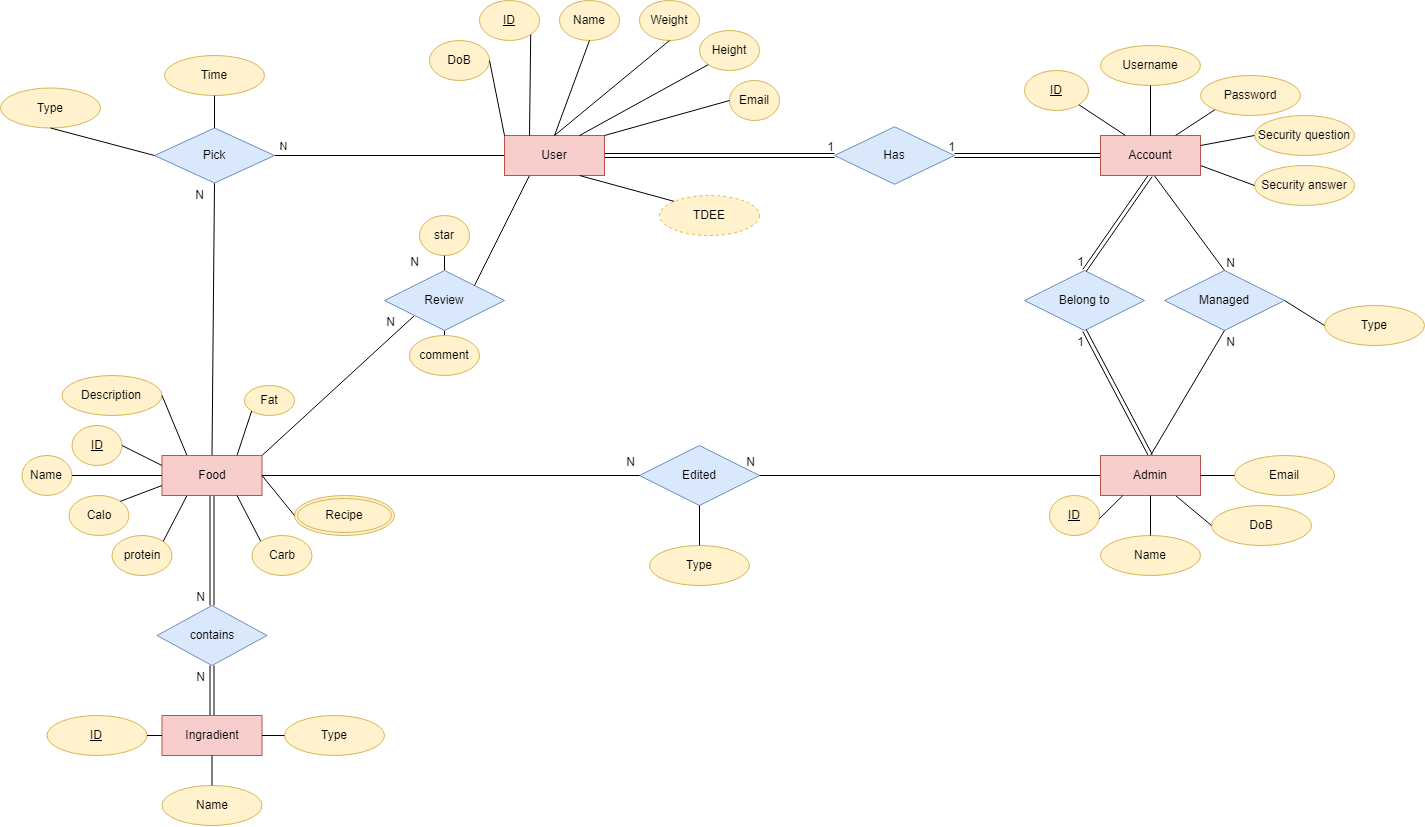
\includegraphics[width=0.99\linewidth]{images/backendDB/Foody_DB-ERD.drawio.png}
            \caption{ER Diagram of FOODY}
        \end{figure}
    \textbf{Link ảnh:} https://drive.google.com/file/d/1lA7-aU0gCllVa-p-Sp3iiUXmH4snUN0m/view?usp=sharing
    \newpage
    \subsection{Mapping}
        \begin{figure}[h]
            \centering
            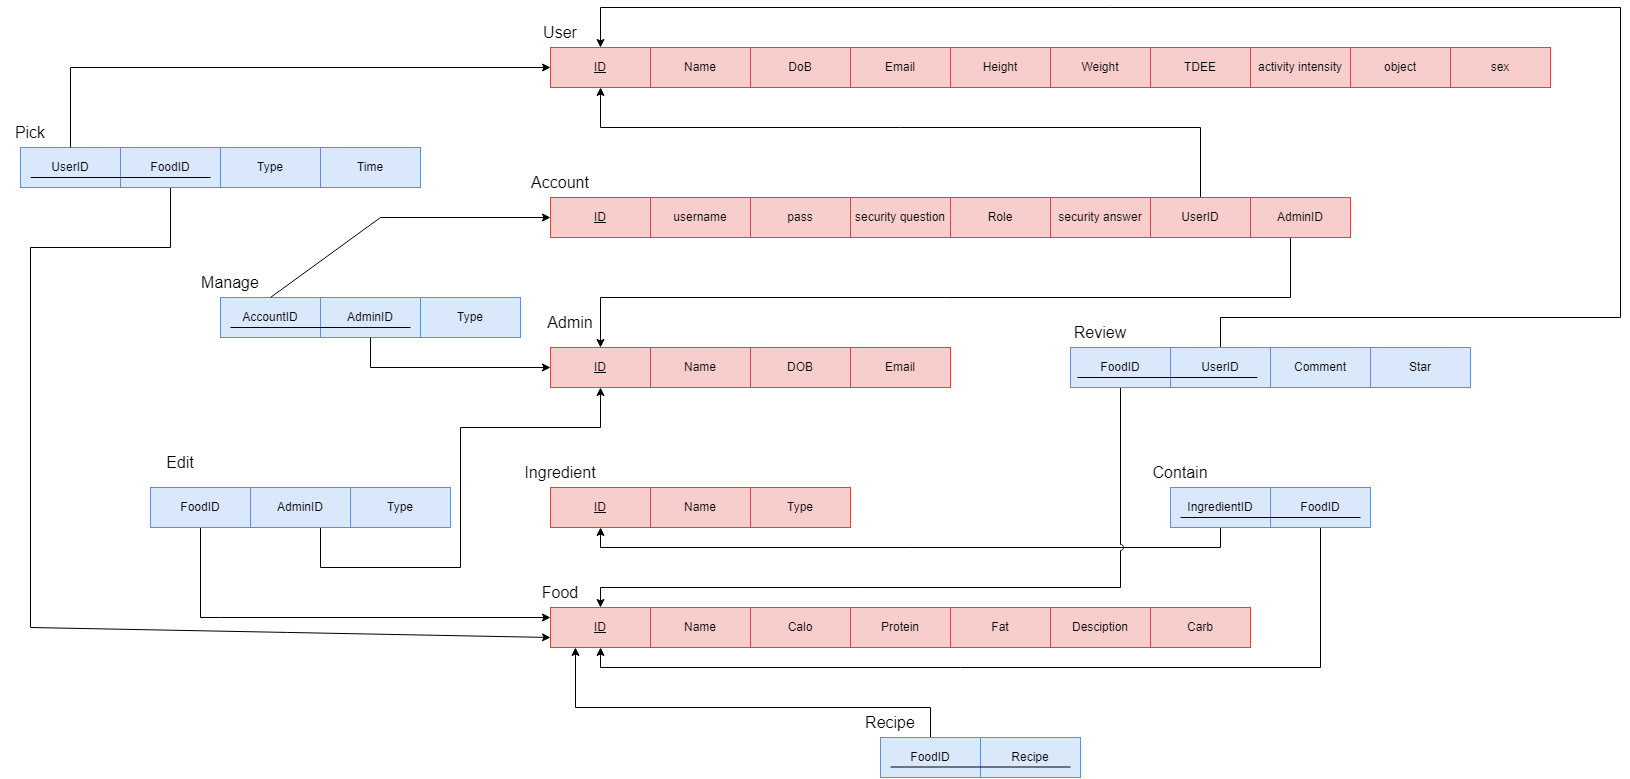
\includegraphics[width=0.99\linewidth]{images/backendDB/Foody_DB-Mapping.drawio.png}
            \caption{Mapping of FOODY}
        \end{figure}
        \textbf{Link ảnh:} https://drive.google.com/file/d/1NyA6kv1SKYCjilm013Aqxx2CA7a8xhSQ/view?usp=sharing
    \newpage
    \subsection{Tables in Mysql}
    Dựa vào thiết kết ý niệm và thiết kế luận lý ở ERD và Mapping ở trên, có thể hiện thực trong Mysql và có kết quả như sau:
        \begin{figure}[h]
            \centering
            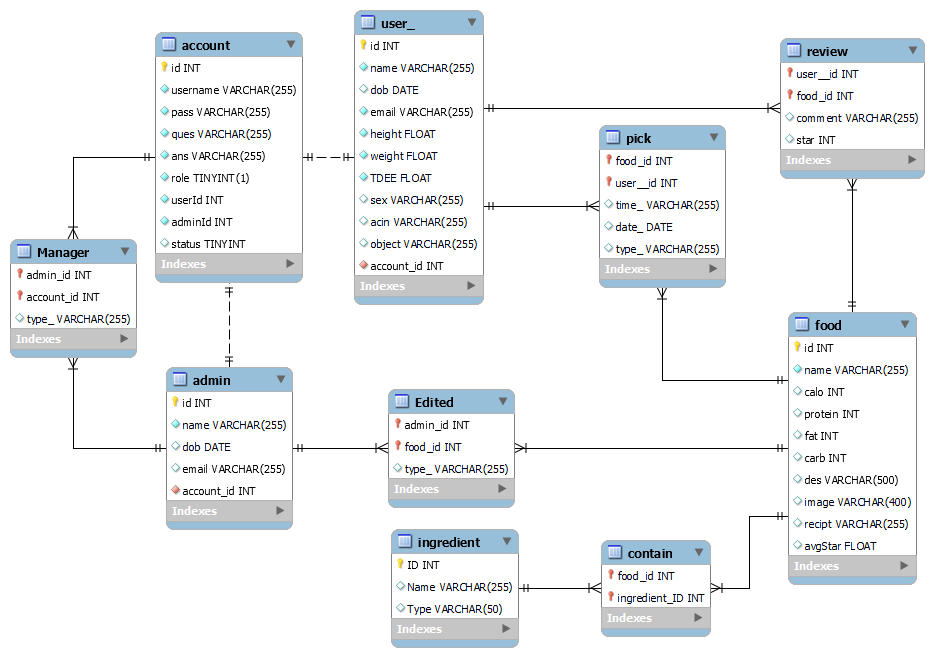
\includegraphics[width=0.99\linewidth]{images/backendDB/sqltable.png}
            \caption{In Mysql}
        \end{figure}
        \textbf{Link ảnh:} https://drive.google.com/file/d/1-6Bw8UxXbeNI\_D4qqNOI5LfYTKBnHXyI/view?usp=sharing
\documentclass[a4paper]{article}
\usepackage[english]{babel}
\usepackage[utf8]{vietnam}
\usepackage{a4wide,amssymb,epsfig,latexsym,multicol,array,hhline,fancyhdr}
\usepackage{amsmath}
\usepackage{lastpage}
\usepackage[lined,boxed,commentsnumbered]{algorithm2e}
\usepackage{enumerate}
\usepackage{color}
\usepackage{graphicx}							
% Standard graphics package
\usepackage{tabularx, caption}
\usepackage{tabularray}
\usepackage{longtable}
\usepackage{multirow}
\usepackage{rotating}
\usepackage{graphics}
\usepackage[a4paper,left=2cm,right=2cm,top=1.8cm,bottom=2.8cm]{geometry}
\usepackage{setspace}
\usepackage{tikz}
\usetikzlibrary{arrows,snakes,backgrounds}
\usepackage[unicode]{hyperref}

%can file puenc.def trong thu muc goc de option [unicode] tao ra bookmark bang tieng Viet
\hypersetup{urlcolor=blue,linkcolor=black,citecolor=black,colorlinks=true} 

\newtheorem{theorem}{{\bf Theorem}}
\newtheorem{property}{{\bf Property}}
\newtheorem{proposition}{{\bf Proposition}}
\newtheorem{corollary}[proposition]{{\bf Corollary}}
\newtheorem{lemma}[proposition]{{\bf Lemma}}

\newcommand\tab[1][0.5cm]{\hspace*{#1}}

\setlength{\headheight}{40pt}
\pagestyle{fancy}
\fancyhead{} % clear all header fields
\fancyhead[L]{
 \begin{tabular}{rl}
    \begin{picture}(25,15)(0,0)
    \put(0,-8){
\includegraphics[width=8mm, height=8mm]{images/hcmut.png}}
    %\put(0,-8){\epsfig{width=10mm,figure=hcmut.eps}}
   \end{picture}&
	%
\includegraphics[width=8mm, height=8mm]{hcmut.png} & %
	\begin{tabular}{l}
		\textbf{\bf \ttfamily Ho Chi Minh City University of Technology, VNU-HCM}\\
		\textbf{\bf \ttfamily Faculty of Computer Science \& Engineering}
	\end{tabular} 	
 \end{tabular}
}
\fancyhead[R]{
	\begin{tabular}{l}
		\tiny \bf \\
		\tiny \bf 
	\end{tabular}  }
\fancyfoot{} % clear all footer fields
\fancyfoot[L]{\scriptsize \ttfamily Đồ án tổng hợp- Hướng công nghệ phần mềm (CO3103), HK 221}
\fancyfoot[R]{\scriptsize \ttfamily Page {\thepage}/\pageref{LastPage}}
\renewcommand{\headrulewidth}{0.3pt}
\renewcommand{\footrulewidth}{0.3pt}


%%%
\setcounter{secnumdepth}{4}
\setcounter{tocdepth}{3}
\makeatletter
\newcounter {subsubsubsection}[subsubsection]
\renewcommand\thesubsubsubsection{\thesubsubsection .\@alph\c@subsubsubsection}
\newcommand\subsubsubsection{\@startsection{subsubsubsection}{4}{\z@}%
                                     {-3.25ex\@plus -1ex \@minus -.2ex}%
                                     {1.5ex \@plus .2ex}%
                                     {\normalfont\normalsize\bfseries}}
\newcommand*\l@subsubsubsection{\@dottedtocline{3}{10.0em}{4.1em}}
\newcommand*{\subsubsubsectionmark}[1]{}
\makeatother

\AtBeginDocument{\renewcommand*\contentsname{Nội dung}}

\begin{document}

\input{sections/title}

\newpage
\tableofcontents

\include{sections/member}
\include{sections/requirement elicitation/main}
\include{sections/use-case diagram/main}
\include{sections/appropriate framework/main}
\include{sections/backendDB/backendDB}
\include{sections/mockup UI/main}
\include{sections/implementation/implementation}

% \inlcude{sections/reference}

\end{document}
\section{Hiện thực và đánh giá ứng dụng}
    \subsection{Yêu cầu phiên bản}
        \begin{enumerate}
            \item \textbf{Backend:}
            \begin{itemize}
                \item Python: v3.10.8
                \item mySQL: v8.0
            \end{itemize}

            \item \textbf{Frontend:}
            \begin{itemize}
                \item NodeJS: v18
                \item React Native: v0.69.6
                \item Expo: v46.0.16
            \end{itemize}

            \item \textbf{Thiết bị hỗ trợ:}
            \begin{itemize}
                \item Các thiết bị sử dụng hệ điều hành Android.
                \item Phiên bản hỗ trợ: Android 10 trở lên.
            \end{itemize}
        \end{enumerate}

    \subsection{Đánh giá ứng dụng}
        \subsubsection{Ưu điểm}
        \begin{enumerate}
            \item Giao diện trực quan, dễ nắm bắt và sử dụng.
            \item Hệ thống hoạt động ổn đinh.
            \item Cá nhân hóa lịch ăn của người dùng dựa trên thông số TDEE và mục tiêu cá nhân.
            \item Người dùng có thể đánh giá cũng như đưa ra những bình luận về món ăn.
            \item Người quản lý có thể quản lý và thực hiện ban những người dùng có những bình luận thiếu ý thức.
            \item Người quản lý có thể chỉnh sửa các món ăn có trong hệ thống.
        \end{enumerate}

        \subsubsection{Nhược điểm}
        \begin{itemize}
            \item Chưa có hướng dẫn từng bước nấu ăn, còn phụ thuộc vào video của bên thứ ba.
            \item Chưa cho phép upload ảnh và video.
            \item Chỉ mới hỗ trợ android, chưa hỗ trợ iOS.
            \item Thiết kế api backend chưa thật sự hiệu quả.
        \end{itemize}

% \inlcude{sections/reference}

\end{document}
\documentclass[a4paper]{article}
\usepackage[english]{babel}
\usepackage[utf8]{vietnam}
\usepackage{a4wide,amssymb,epsfig,latexsym,multicol,array,hhline,fancyhdr}
\usepackage{amsmath}
\usepackage{lastpage}
\usepackage[lined,boxed,commentsnumbered]{algorithm2e}
\usepackage{enumerate}
\usepackage{color}
\usepackage{graphicx}							
% Standard graphics package
\usepackage{tabularx, caption}
\usepackage{tabularray}
\usepackage{longtable}
\usepackage{multirow}
\usepackage{rotating}
\usepackage{graphics}
\usepackage[a4paper,left=2cm,right=2cm,top=1.8cm,bottom=2.8cm]{geometry}
\usepackage{setspace}
\usepackage{tikz}
\usetikzlibrary{arrows,snakes,backgrounds}
\usepackage[unicode]{hyperref}

%can file puenc.def trong thu muc goc de option [unicode] tao ra bookmark bang tieng Viet
\hypersetup{urlcolor=blue,linkcolor=black,citecolor=black,colorlinks=true} 

\newtheorem{theorem}{{\bf Theorem}}
\newtheorem{property}{{\bf Property}}
\newtheorem{proposition}{{\bf Proposition}}
\newtheorem{corollary}[proposition]{{\bf Corollary}}
\newtheorem{lemma}[proposition]{{\bf Lemma}}

\newcommand\tab[1][0.5cm]{\hspace*{#1}}

\setlength{\headheight}{40pt}
\pagestyle{fancy}
\fancyhead{} % clear all header fields
\fancyhead[L]{
 \begin{tabular}{rl}
    \begin{picture}(25,15)(0,0)
    \put(0,-8){
\includegraphics[width=8mm, height=8mm]{images/hcmut.png}}
    %\put(0,-8){\epsfig{width=10mm,figure=hcmut.eps}}
   \end{picture}&
	%
\includegraphics[width=8mm, height=8mm]{hcmut.png} & %
	\begin{tabular}{l}
		\textbf{\bf \ttfamily Ho Chi Minh City University of Technology, VNU-HCM}\\
		\textbf{\bf \ttfamily Faculty of Computer Science \& Engineering}
	\end{tabular} 	
 \end{tabular}
}
\fancyhead[R]{
	\begin{tabular}{l}
		\tiny \bf \\
		\tiny \bf 
	\end{tabular}  }
\fancyfoot{} % clear all footer fields
\fancyfoot[L]{\scriptsize \ttfamily Đồ án tổng hợp- Hướng công nghệ phần mềm (CO3103), HK 221}
\fancyfoot[R]{\scriptsize \ttfamily Page {\thepage}/\pageref{LastPage}}
\renewcommand{\headrulewidth}{0.3pt}
\renewcommand{\footrulewidth}{0.3pt}


%%%
\setcounter{secnumdepth}{4}
\setcounter{tocdepth}{3}
\makeatletter
\newcounter {subsubsubsection}[subsubsection]
\renewcommand\thesubsubsubsection{\thesubsubsection .\@alph\c@subsubsubsection}
\newcommand\subsubsubsection{\@startsection{subsubsubsection}{4}{\z@}%
                                     {-3.25ex\@plus -1ex \@minus -.2ex}%
                                     {1.5ex \@plus .2ex}%
                                     {\normalfont\normalsize\bfseries}}
\newcommand*\l@subsubsubsection{\@dottedtocline{3}{10.0em}{4.1em}}
\newcommand*{\subsubsubsectionmark}[1]{}
\makeatother

\AtBeginDocument{\renewcommand*\contentsname{Nội dung}}

\begin{document}


\graphicspath{{\subfix{../images/}}}
\begin{titlepage}

\begin{center}
    \large
    ĐẠI HỌC QUỐC GIA THÀNH PHỐ HỒ CHÍ MINH \\
    TRƯỜNG ĐẠI HỌC BÁCH KHOA \\
    KHOA KHOA HỌC VÀ KỸ THUẬT MÁY TÍNH \\
\end{center}

\vspace{1cm}

\begin{figure}[h!]
\begin{center}

\includegraphics[width=3cm]{images/hcmut.png}
\end{center}
\end{figure}

\vspace{1cm}


\begin{center}
\begin{tabular}{c}
\multicolumn{1}{l}{\textbf{{\Large ĐỒ ÁN TỔNG HỢP- HƯỚNG CÔNG NGHỆ PHẦN MỀM}}}\\
~~\\
\hline
\\
\multicolumn{1}{l}{\textbf{{\Large Report}}}\\
\\
\textbf{\Large ỨNG DỤNG ĐỀ XUẤT MÓN ĂN} \\ \textbf{\Large PHÙ HỢP VỚI NGƯỜI DÙNG (FOODY)}\\
\\
\hline
\end{tabular}
\end{center}

\vspace{3cm}

\begin{table}[h]
\begin{tabular}{rrl}

\hspace{5 cm} & GVHD: &\textbf{Lê Đình Thuận} \\
& & \textbf{Mai Đức Trung} \\
& Lớp: &L01 \\
& Thành viên: & - Lê Nguyễn Huyền Thoại - 2012122 \textbf{(Nhóm trưởng)} \\
& &  - Lê Văn Bằng - 2012684\\
& &  - Nguyễn Ngọc Hùng - 2013368 \\
& &  - Lê Trí Nguyên - 2013913 \\
& &  - Trần Văn Kiên - 2013552 \\

\end{tabular}
\end{table}

\vspace{4cm}
\begin{center}
{\footnotesize Hồ Chí Minh, 09/2022}
\end{center}
\end{titlepage}

\newpage
\tableofcontents

\section{Danh sách thành viên \& Khối lượng công việc}

\begin{tblr}{
    width=1\linewidth,
    hlines,
    vlines,
    colspec={X[-2]X[4]X[1.5]X[6]X[-1]},
    columns = {valign = m, },
    column{1} = {halign = c, },
    row{1} = {halign = c, valign = m, bg = lightgray, fg = black},
}
    {\textbf{STT} & \textbf{Họ và tên} & \textbf{MSSV} & \textbf{Công việc} & \textbf{Hoàn thành} }  \\
    1 & Lê Nguyễn Huyền Thoại & 2012122 & - Quản lý tiến độ công việc \newline
                                          - Thiểt kế use-case diagram gợi ý món ăn \newline
                                          - Thiết kế UI \newline
                                          - Hiện thực phần user view front end
                                        & 100\% \\
    2 & Lê Văn Bằng           & 2012684 & - Xác định yêu cầu phi chức năng \newline
                                          - Viết mô tả cho use-case diagram \newline
                                          - Hiện thực phần authentication front end
                                        & 100\% \\
    3 & Nguyễn Ngọc Hùng	  & 2013368 & - Xác định yêu cầu chức năng \newline
                                          - Thiết kế use-case xác thực \newline
                                          - Thiết kế database \newline
                                          - Hiện thực backend \newline
                                        & 100\% \\
    4 & Lê Trí Nguyên         & 2013913 & - Thiết kế use-case diagram tổng \newline
                                          - Thiết kế database \newline
                                          - Hiện thực backend \newline
                                        & 100\% \\
    5 & Trần Văn Kiên         & 2013552 & - Xác định ngữ cảnh và yêu cầu phi chức năng \newline
                                          - Tìm hiểu công nghệ \newline
                                          - Hiện thực phần admin-view front end
                                        & 100\% \\

\end{tblr}

\documentclass[a4paper]{article}
\usepackage[english]{babel}
\usepackage[utf8]{vietnam}
\usepackage{a4wide,amssymb,epsfig,latexsym,multicol,array,hhline,fancyhdr}
\usepackage{amsmath}
\usepackage{lastpage}
\usepackage[lined,boxed,commentsnumbered]{algorithm2e}
\usepackage{enumerate}
\usepackage{color}
\usepackage{graphicx}							
% Standard graphics package
\usepackage{tabularx, caption}
\usepackage{tabularray}
\usepackage{longtable}
\usepackage{multirow}
\usepackage{rotating}
\usepackage{graphics}
\usepackage[a4paper,left=2cm,right=2cm,top=1.8cm,bottom=2.8cm]{geometry}
\usepackage{setspace}
\usepackage{tikz}
\usetikzlibrary{arrows,snakes,backgrounds}
\usepackage[unicode]{hyperref}

%can file puenc.def trong thu muc goc de option [unicode] tao ra bookmark bang tieng Viet
\hypersetup{urlcolor=blue,linkcolor=black,citecolor=black,colorlinks=true} 

\newtheorem{theorem}{{\bf Theorem}}
\newtheorem{property}{{\bf Property}}
\newtheorem{proposition}{{\bf Proposition}}
\newtheorem{corollary}[proposition]{{\bf Corollary}}
\newtheorem{lemma}[proposition]{{\bf Lemma}}

\newcommand\tab[1][0.5cm]{\hspace*{#1}}

\setlength{\headheight}{40pt}
\pagestyle{fancy}
\fancyhead{} % clear all header fields
\fancyhead[L]{
 \begin{tabular}{rl}
    \begin{picture}(25,15)(0,0)
    \put(0,-8){
\includegraphics[width=8mm, height=8mm]{images/hcmut.png}}
    %\put(0,-8){\epsfig{width=10mm,figure=hcmut.eps}}
   \end{picture}&
	%
\includegraphics[width=8mm, height=8mm]{hcmut.png} & %
	\begin{tabular}{l}
		\textbf{\bf \ttfamily Ho Chi Minh City University of Technology, VNU-HCM}\\
		\textbf{\bf \ttfamily Faculty of Computer Science \& Engineering}
	\end{tabular} 	
 \end{tabular}
}
\fancyhead[R]{
	\begin{tabular}{l}
		\tiny \bf \\
		\tiny \bf 
	\end{tabular}  }
\fancyfoot{} % clear all footer fields
\fancyfoot[L]{\scriptsize \ttfamily Đồ án tổng hợp- Hướng công nghệ phần mềm (CO3103), HK 221}
\fancyfoot[R]{\scriptsize \ttfamily Page {\thepage}/\pageref{LastPage}}
\renewcommand{\headrulewidth}{0.3pt}
\renewcommand{\footrulewidth}{0.3pt}


%%%
\setcounter{secnumdepth}{4}
\setcounter{tocdepth}{3}
\makeatletter
\newcounter {subsubsubsection}[subsubsection]
\renewcommand\thesubsubsubsection{\thesubsubsection .\@alph\c@subsubsubsection}
\newcommand\subsubsubsection{\@startsection{subsubsubsection}{4}{\z@}%
                                     {-3.25ex\@plus -1ex \@minus -.2ex}%
                                     {1.5ex \@plus .2ex}%
                                     {\normalfont\normalsize\bfseries}}
\newcommand*\l@subsubsubsection{\@dottedtocline{3}{10.0em}{4.1em}}
\newcommand*{\subsubsubsectionmark}[1]{}
\makeatother

\AtBeginDocument{\renewcommand*\contentsname{Nội dung}}

\begin{document}

\input{sections/title}

\newpage
\tableofcontents

\include{sections/member}
\include{sections/requirement elicitation/main}
\include{sections/use-case diagram/main}
\include{sections/appropriate framework/main}
\include{sections/backendDB/backendDB}
\include{sections/mockup UI/main}
\include{sections/implementation/implementation}

% \inlcude{sections/reference}

\end{document}
\documentclass[a4paper]{article}
\usepackage[english]{babel}
\usepackage[utf8]{vietnam}
\usepackage{a4wide,amssymb,epsfig,latexsym,multicol,array,hhline,fancyhdr}
\usepackage{amsmath}
\usepackage{lastpage}
\usepackage[lined,boxed,commentsnumbered]{algorithm2e}
\usepackage{enumerate}
\usepackage{color}
\usepackage{graphicx}							
% Standard graphics package
\usepackage{tabularx, caption}
\usepackage{tabularray}
\usepackage{longtable}
\usepackage{multirow}
\usepackage{rotating}
\usepackage{graphics}
\usepackage[a4paper,left=2cm,right=2cm,top=1.8cm,bottom=2.8cm]{geometry}
\usepackage{setspace}
\usepackage{tikz}
\usetikzlibrary{arrows,snakes,backgrounds}
\usepackage[unicode]{hyperref}

%can file puenc.def trong thu muc goc de option [unicode] tao ra bookmark bang tieng Viet
\hypersetup{urlcolor=blue,linkcolor=black,citecolor=black,colorlinks=true} 

\newtheorem{theorem}{{\bf Theorem}}
\newtheorem{property}{{\bf Property}}
\newtheorem{proposition}{{\bf Proposition}}
\newtheorem{corollary}[proposition]{{\bf Corollary}}
\newtheorem{lemma}[proposition]{{\bf Lemma}}

\newcommand\tab[1][0.5cm]{\hspace*{#1}}

\setlength{\headheight}{40pt}
\pagestyle{fancy}
\fancyhead{} % clear all header fields
\fancyhead[L]{
 \begin{tabular}{rl}
    \begin{picture}(25,15)(0,0)
    \put(0,-8){
\includegraphics[width=8mm, height=8mm]{images/hcmut.png}}
    %\put(0,-8){\epsfig{width=10mm,figure=hcmut.eps}}
   \end{picture}&
	%
\includegraphics[width=8mm, height=8mm]{hcmut.png} & %
	\begin{tabular}{l}
		\textbf{\bf \ttfamily Ho Chi Minh City University of Technology, VNU-HCM}\\
		\textbf{\bf \ttfamily Faculty of Computer Science \& Engineering}
	\end{tabular} 	
 \end{tabular}
}
\fancyhead[R]{
	\begin{tabular}{l}
		\tiny \bf \\
		\tiny \bf 
	\end{tabular}  }
\fancyfoot{} % clear all footer fields
\fancyfoot[L]{\scriptsize \ttfamily Đồ án tổng hợp- Hướng công nghệ phần mềm (CO3103), HK 221}
\fancyfoot[R]{\scriptsize \ttfamily Page {\thepage}/\pageref{LastPage}}
\renewcommand{\headrulewidth}{0.3pt}
\renewcommand{\footrulewidth}{0.3pt}


%%%
\setcounter{secnumdepth}{4}
\setcounter{tocdepth}{3}
\makeatletter
\newcounter {subsubsubsection}[subsubsection]
\renewcommand\thesubsubsubsection{\thesubsubsection .\@alph\c@subsubsubsection}
\newcommand\subsubsubsection{\@startsection{subsubsubsection}{4}{\z@}%
                                     {-3.25ex\@plus -1ex \@minus -.2ex}%
                                     {1.5ex \@plus .2ex}%
                                     {\normalfont\normalsize\bfseries}}
\newcommand*\l@subsubsubsection{\@dottedtocline{3}{10.0em}{4.1em}}
\newcommand*{\subsubsubsectionmark}[1]{}
\makeatother

\AtBeginDocument{\renewcommand*\contentsname{Nội dung}}

\begin{document}

\input{sections/title}

\newpage
\tableofcontents

\include{sections/member}
\include{sections/requirement elicitation/main}
\include{sections/use-case diagram/main}
\include{sections/appropriate framework/main}
\include{sections/backendDB/backendDB}
\include{sections/mockup UI/main}
\include{sections/implementation/implementation}

% \inlcude{sections/reference}

\end{document}
\documentclass[a4paper]{article}
\usepackage[english]{babel}
\usepackage[utf8]{vietnam}
\usepackage{a4wide,amssymb,epsfig,latexsym,multicol,array,hhline,fancyhdr}
\usepackage{amsmath}
\usepackage{lastpage}
\usepackage[lined,boxed,commentsnumbered]{algorithm2e}
\usepackage{enumerate}
\usepackage{color}
\usepackage{graphicx}							
% Standard graphics package
\usepackage{tabularx, caption}
\usepackage{tabularray}
\usepackage{longtable}
\usepackage{multirow}
\usepackage{rotating}
\usepackage{graphics}
\usepackage[a4paper,left=2cm,right=2cm,top=1.8cm,bottom=2.8cm]{geometry}
\usepackage{setspace}
\usepackage{tikz}
\usetikzlibrary{arrows,snakes,backgrounds}
\usepackage[unicode]{hyperref}

%can file puenc.def trong thu muc goc de option [unicode] tao ra bookmark bang tieng Viet
\hypersetup{urlcolor=blue,linkcolor=black,citecolor=black,colorlinks=true} 

\newtheorem{theorem}{{\bf Theorem}}
\newtheorem{property}{{\bf Property}}
\newtheorem{proposition}{{\bf Proposition}}
\newtheorem{corollary}[proposition]{{\bf Corollary}}
\newtheorem{lemma}[proposition]{{\bf Lemma}}

\newcommand\tab[1][0.5cm]{\hspace*{#1}}

\setlength{\headheight}{40pt}
\pagestyle{fancy}
\fancyhead{} % clear all header fields
\fancyhead[L]{
 \begin{tabular}{rl}
    \begin{picture}(25,15)(0,0)
    \put(0,-8){
\includegraphics[width=8mm, height=8mm]{images/hcmut.png}}
    %\put(0,-8){\epsfig{width=10mm,figure=hcmut.eps}}
   \end{picture}&
	%
\includegraphics[width=8mm, height=8mm]{hcmut.png} & %
	\begin{tabular}{l}
		\textbf{\bf \ttfamily Ho Chi Minh City University of Technology, VNU-HCM}\\
		\textbf{\bf \ttfamily Faculty of Computer Science \& Engineering}
	\end{tabular} 	
 \end{tabular}
}
\fancyhead[R]{
	\begin{tabular}{l}
		\tiny \bf \\
		\tiny \bf 
	\end{tabular}  }
\fancyfoot{} % clear all footer fields
\fancyfoot[L]{\scriptsize \ttfamily Đồ án tổng hợp- Hướng công nghệ phần mềm (CO3103), HK 221}
\fancyfoot[R]{\scriptsize \ttfamily Page {\thepage}/\pageref{LastPage}}
\renewcommand{\headrulewidth}{0.3pt}
\renewcommand{\footrulewidth}{0.3pt}


%%%
\setcounter{secnumdepth}{4}
\setcounter{tocdepth}{3}
\makeatletter
\newcounter {subsubsubsection}[subsubsection]
\renewcommand\thesubsubsubsection{\thesubsubsection .\@alph\c@subsubsubsection}
\newcommand\subsubsubsection{\@startsection{subsubsubsection}{4}{\z@}%
                                     {-3.25ex\@plus -1ex \@minus -.2ex}%
                                     {1.5ex \@plus .2ex}%
                                     {\normalfont\normalsize\bfseries}}
\newcommand*\l@subsubsubsection{\@dottedtocline{3}{10.0em}{4.1em}}
\newcommand*{\subsubsubsectionmark}[1]{}
\makeatother

\AtBeginDocument{\renewcommand*\contentsname{Nội dung}}

\begin{document}

\input{sections/title}

\newpage
\tableofcontents

\include{sections/member}
\include{sections/requirement elicitation/main}
\include{sections/use-case diagram/main}
\include{sections/appropriate framework/main}
\include{sections/backendDB/backendDB}
\include{sections/mockup UI/main}
\include{sections/implementation/implementation}

% \inlcude{sections/reference}

\end{document}
\section{Hiện thực Database}
    \subsection{ER Diagram}
    Dựa vào Use-case Diagram kèm theo các mô tả cho từng use-case ở phần 2. Xác định được các thực thể và mối quan hệ cho Database như sau:
        \begin{itemize}
            \item Thực thể: \textbf{User}, \textbf{account}, \textbf{admin}, \textbf{food}, \textbf{ingredient}.
            \item Mối quan hệ: User-\textbf{review}-food, User-\textbf{pick}-food, food-\textbf{contain}-ingredient, admin-\textbf{edited}-food, account-\textbf{belongto}-admin, admin-\textbf{manage}-account.
        \end{itemize}
        \begin{figure}[h]
            \centering
            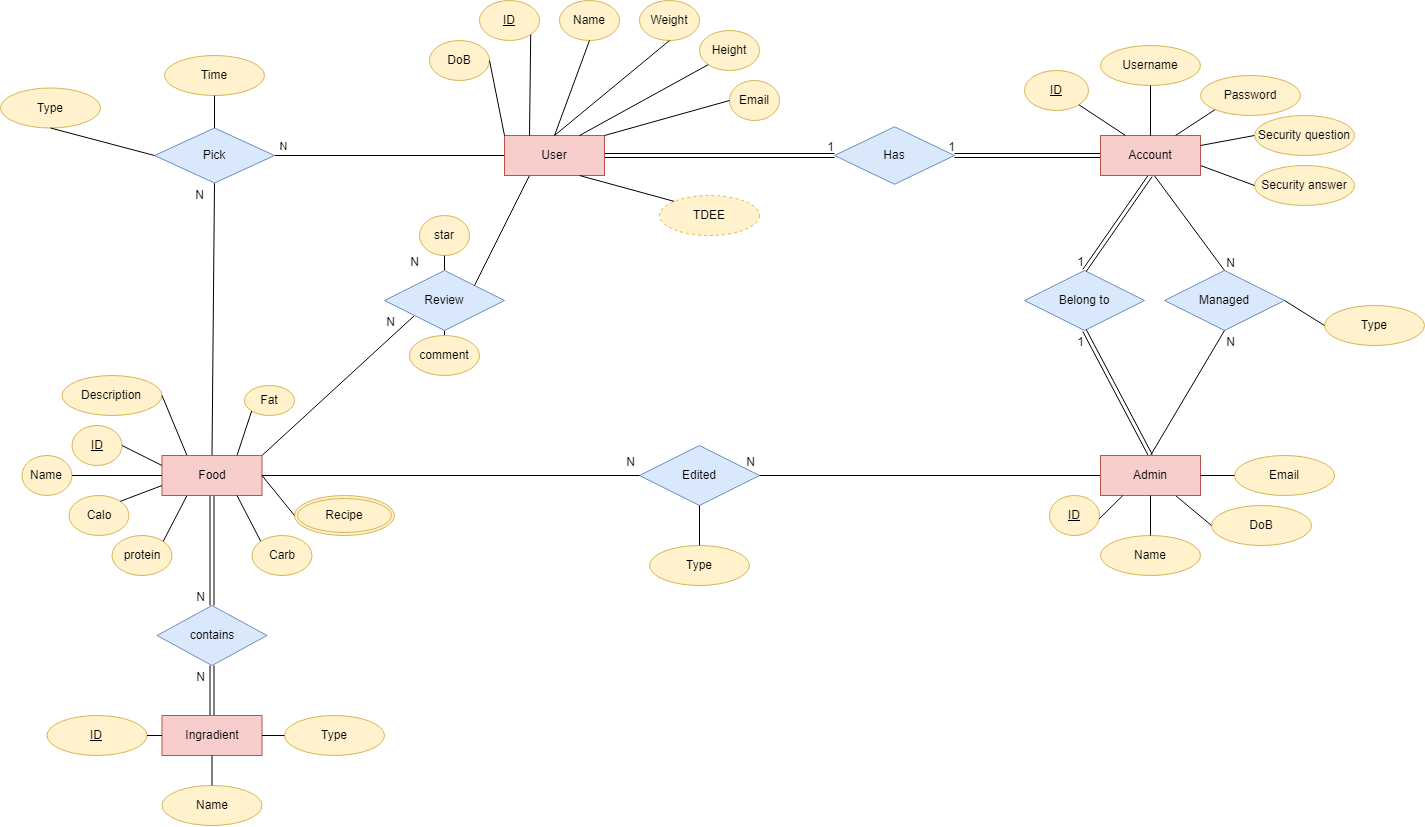
\includegraphics[width=0.99\linewidth]{images/backendDB/Foody_DB-ERD.drawio.png}
            \caption{ER Diagram of FOODY}
        \end{figure}
    \textbf{Link ảnh:} https://drive.google.com/file/d/1lA7-aU0gCllVa-p-Sp3iiUXmH4snUN0m/view?usp=sharing
    \newpage
    \subsection{Mapping}
        \begin{figure}[h]
            \centering
            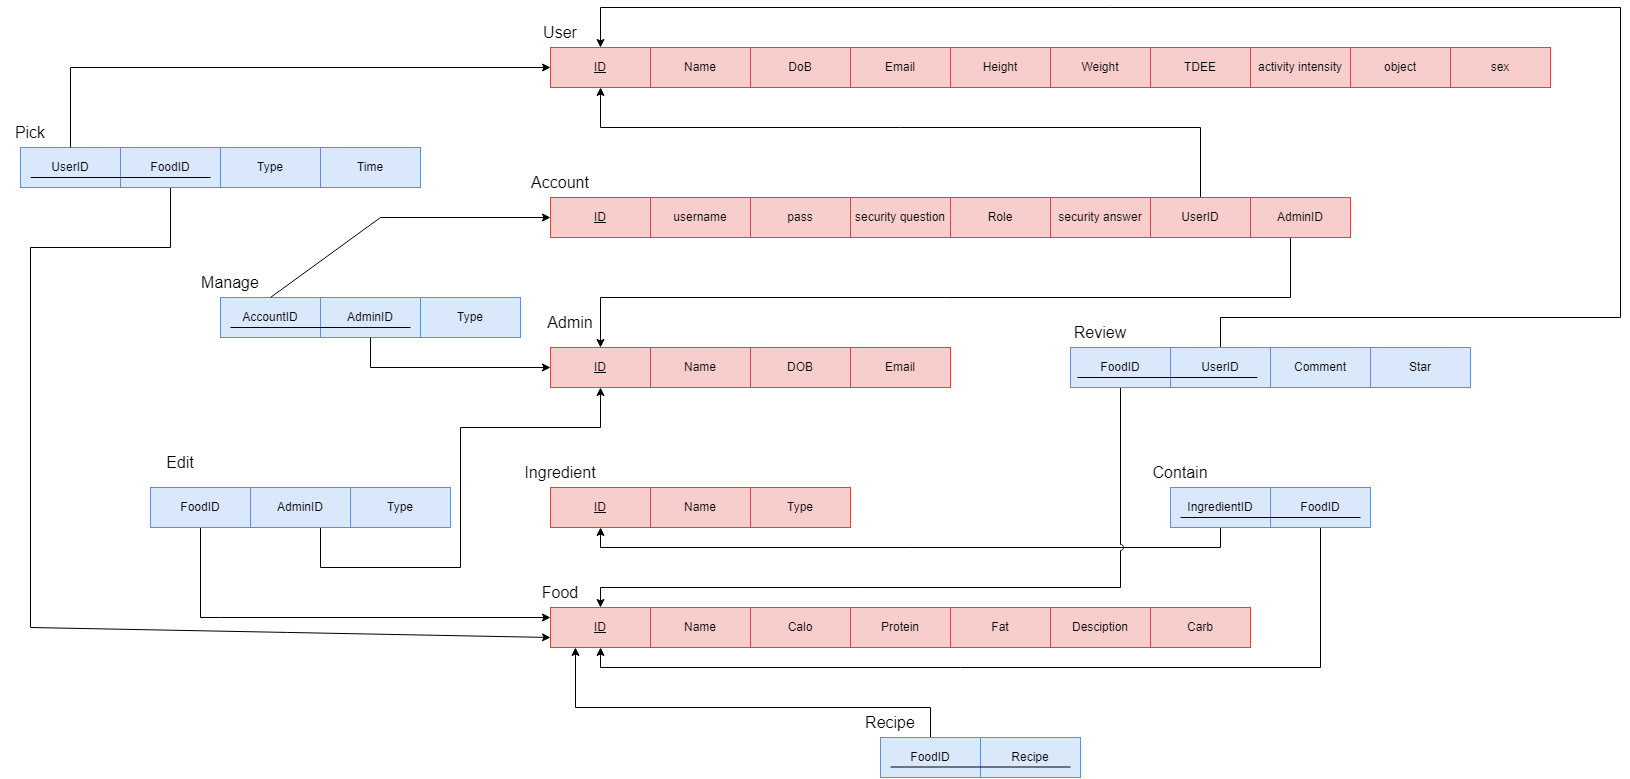
\includegraphics[width=0.99\linewidth]{images/backendDB/Foody_DB-Mapping.drawio.png}
            \caption{Mapping of FOODY}
        \end{figure}
        \textbf{Link ảnh:} https://drive.google.com/file/d/1NyA6kv1SKYCjilm013Aqxx2CA7a8xhSQ/view?usp=sharing
    \newpage
    \subsection{Tables in Mysql}
    Dựa vào thiết kết ý niệm và thiết kế luận lý ở ERD và Mapping ở trên, có thể hiện thực trong Mysql và có kết quả như sau:
        \begin{figure}[h]
            \centering
            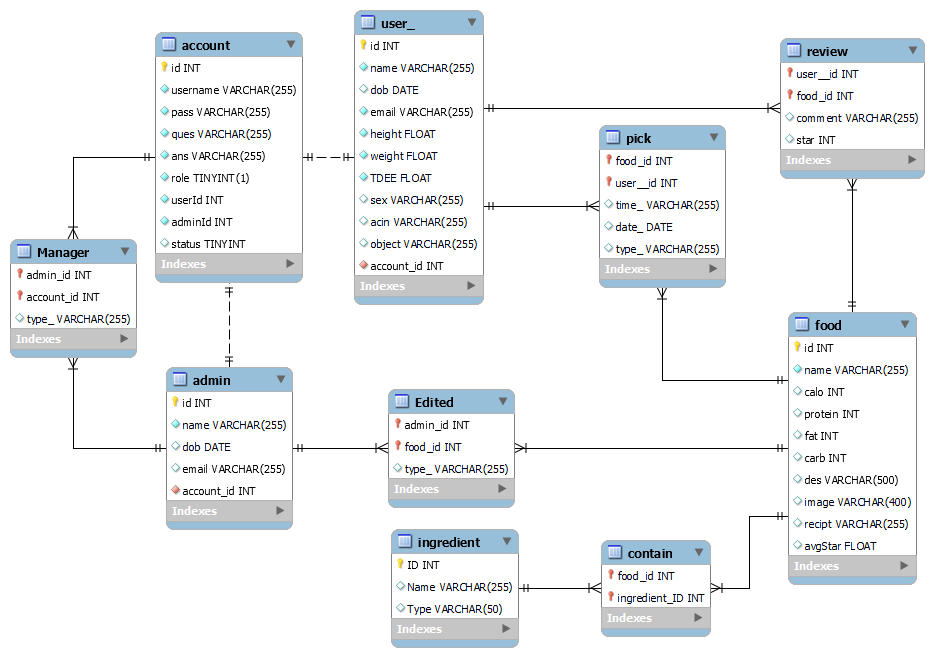
\includegraphics[width=0.99\linewidth]{images/backendDB/sqltable.png}
            \caption{In Mysql}
        \end{figure}
        \textbf{Link ảnh:} https://drive.google.com/file/d/1-6Bw8UxXbeNI\_D4qqNOI5LfYTKBnHXyI/view?usp=sharing
\documentclass[a4paper]{article}
\usepackage[english]{babel}
\usepackage[utf8]{vietnam}
\usepackage{a4wide,amssymb,epsfig,latexsym,multicol,array,hhline,fancyhdr}
\usepackage{amsmath}
\usepackage{lastpage}
\usepackage[lined,boxed,commentsnumbered]{algorithm2e}
\usepackage{enumerate}
\usepackage{color}
\usepackage{graphicx}							
% Standard graphics package
\usepackage{tabularx, caption}
\usepackage{tabularray}
\usepackage{longtable}
\usepackage{multirow}
\usepackage{rotating}
\usepackage{graphics}
\usepackage[a4paper,left=2cm,right=2cm,top=1.8cm,bottom=2.8cm]{geometry}
\usepackage{setspace}
\usepackage{tikz}
\usetikzlibrary{arrows,snakes,backgrounds}
\usepackage[unicode]{hyperref}

%can file puenc.def trong thu muc goc de option [unicode] tao ra bookmark bang tieng Viet
\hypersetup{urlcolor=blue,linkcolor=black,citecolor=black,colorlinks=true} 

\newtheorem{theorem}{{\bf Theorem}}
\newtheorem{property}{{\bf Property}}
\newtheorem{proposition}{{\bf Proposition}}
\newtheorem{corollary}[proposition]{{\bf Corollary}}
\newtheorem{lemma}[proposition]{{\bf Lemma}}

\newcommand\tab[1][0.5cm]{\hspace*{#1}}

\setlength{\headheight}{40pt}
\pagestyle{fancy}
\fancyhead{} % clear all header fields
\fancyhead[L]{
 \begin{tabular}{rl}
    \begin{picture}(25,15)(0,0)
    \put(0,-8){
\includegraphics[width=8mm, height=8mm]{images/hcmut.png}}
    %\put(0,-8){\epsfig{width=10mm,figure=hcmut.eps}}
   \end{picture}&
	%
\includegraphics[width=8mm, height=8mm]{hcmut.png} & %
	\begin{tabular}{l}
		\textbf{\bf \ttfamily Ho Chi Minh City University of Technology, VNU-HCM}\\
		\textbf{\bf \ttfamily Faculty of Computer Science \& Engineering}
	\end{tabular} 	
 \end{tabular}
}
\fancyhead[R]{
	\begin{tabular}{l}
		\tiny \bf \\
		\tiny \bf 
	\end{tabular}  }
\fancyfoot{} % clear all footer fields
\fancyfoot[L]{\scriptsize \ttfamily Đồ án tổng hợp- Hướng công nghệ phần mềm (CO3103), HK 221}
\fancyfoot[R]{\scriptsize \ttfamily Page {\thepage}/\pageref{LastPage}}
\renewcommand{\headrulewidth}{0.3pt}
\renewcommand{\footrulewidth}{0.3pt}


%%%
\setcounter{secnumdepth}{4}
\setcounter{tocdepth}{3}
\makeatletter
\newcounter {subsubsubsection}[subsubsection]
\renewcommand\thesubsubsubsection{\thesubsubsection .\@alph\c@subsubsubsection}
\newcommand\subsubsubsection{\@startsection{subsubsubsection}{4}{\z@}%
                                     {-3.25ex\@plus -1ex \@minus -.2ex}%
                                     {1.5ex \@plus .2ex}%
                                     {\normalfont\normalsize\bfseries}}
\newcommand*\l@subsubsubsection{\@dottedtocline{3}{10.0em}{4.1em}}
\newcommand*{\subsubsubsectionmark}[1]{}
\makeatother

\AtBeginDocument{\renewcommand*\contentsname{Nội dung}}

\begin{document}

\input{sections/title}

\newpage
\tableofcontents

\include{sections/member}
\include{sections/requirement elicitation/main}
\include{sections/use-case diagram/main}
\include{sections/appropriate framework/main}
\include{sections/backendDB/backendDB}
\include{sections/mockup UI/main}
\include{sections/implementation/implementation}

% \inlcude{sections/reference}

\end{document}
\section{Hiện thực và đánh giá ứng dụng}
    \subsection{Yêu cầu phiên bản}
        \begin{enumerate}
            \item \textbf{Backend:}
            \begin{itemize}
                \item Python: v3.10.8
                \item mySQL: v8.0
            \end{itemize}

            \item \textbf{Frontend:}
            \begin{itemize}
                \item NodeJS: v18
                \item React Native: v0.69.6
                \item Expo: v46.0.16
            \end{itemize}

            \item \textbf{Thiết bị hỗ trợ:}
            \begin{itemize}
                \item Các thiết bị sử dụng hệ điều hành Android.
                \item Phiên bản hỗ trợ: Android 10 trở lên.
            \end{itemize}
        \end{enumerate}

    \subsection{Đánh giá ứng dụng}
        \subsubsection{Ưu điểm}
        \begin{enumerate}
            \item Giao diện trực quan, dễ nắm bắt và sử dụng.
            \item Hệ thống hoạt động ổn đinh.
            \item Cá nhân hóa lịch ăn của người dùng dựa trên thông số TDEE và mục tiêu cá nhân.
            \item Người dùng có thể đánh giá cũng như đưa ra những bình luận về món ăn.
            \item Người quản lý có thể quản lý và thực hiện ban những người dùng có những bình luận thiếu ý thức.
            \item Người quản lý có thể chỉnh sửa các món ăn có trong hệ thống.
        \end{enumerate}

        \subsubsection{Nhược điểm}
        \begin{itemize}
            \item Chưa có hướng dẫn từng bước nấu ăn, còn phụ thuộc vào video của bên thứ ba.
            \item Chưa cho phép upload ảnh và video.
            \item Chỉ mới hỗ trợ android, chưa hỗ trợ iOS.
            \item Thiết kế api backend chưa thật sự hiệu quả.
        \end{itemize}

% \inlcude{sections/reference}

\end{document}
\documentclass[a4paper]{article}
\usepackage[english]{babel}
\usepackage[utf8]{vietnam}
\usepackage{a4wide,amssymb,epsfig,latexsym,multicol,array,hhline,fancyhdr}
\usepackage{amsmath}
\usepackage{lastpage}
\usepackage[lined,boxed,commentsnumbered]{algorithm2e}
\usepackage{enumerate}
\usepackage{color}
\usepackage{graphicx}							
% Standard graphics package
\usepackage{tabularx, caption}
\usepackage{tabularray}
\usepackage{longtable}
\usepackage{multirow}
\usepackage{rotating}
\usepackage{graphics}
\usepackage[a4paper,left=2cm,right=2cm,top=1.8cm,bottom=2.8cm]{geometry}
\usepackage{setspace}
\usepackage{tikz}
\usetikzlibrary{arrows,snakes,backgrounds}
\usepackage[unicode]{hyperref}

%can file puenc.def trong thu muc goc de option [unicode] tao ra bookmark bang tieng Viet
\hypersetup{urlcolor=blue,linkcolor=black,citecolor=black,colorlinks=true} 

\newtheorem{theorem}{{\bf Theorem}}
\newtheorem{property}{{\bf Property}}
\newtheorem{proposition}{{\bf Proposition}}
\newtheorem{corollary}[proposition]{{\bf Corollary}}
\newtheorem{lemma}[proposition]{{\bf Lemma}}

\newcommand\tab[1][0.5cm]{\hspace*{#1}}

\setlength{\headheight}{40pt}
\pagestyle{fancy}
\fancyhead{} % clear all header fields
\fancyhead[L]{
 \begin{tabular}{rl}
    \begin{picture}(25,15)(0,0)
    \put(0,-8){
\includegraphics[width=8mm, height=8mm]{images/hcmut.png}}
    %\put(0,-8){\epsfig{width=10mm,figure=hcmut.eps}}
   \end{picture}&
	%
\includegraphics[width=8mm, height=8mm]{hcmut.png} & %
	\begin{tabular}{l}
		\textbf{\bf \ttfamily Ho Chi Minh City University of Technology, VNU-HCM}\\
		\textbf{\bf \ttfamily Faculty of Computer Science \& Engineering}
	\end{tabular} 	
 \end{tabular}
}
\fancyhead[R]{
	\begin{tabular}{l}
		\tiny \bf \\
		\tiny \bf 
	\end{tabular}  }
\fancyfoot{} % clear all footer fields
\fancyfoot[L]{\scriptsize \ttfamily Đồ án tổng hợp- Hướng công nghệ phần mềm (CO3103), HK 221}
\fancyfoot[R]{\scriptsize \ttfamily Page {\thepage}/\pageref{LastPage}}
\renewcommand{\headrulewidth}{0.3pt}
\renewcommand{\footrulewidth}{0.3pt}


%%%
\setcounter{secnumdepth}{4}
\setcounter{tocdepth}{3}
\makeatletter
\newcounter {subsubsubsection}[subsubsection]
\renewcommand\thesubsubsubsection{\thesubsubsection .\@alph\c@subsubsubsection}
\newcommand\subsubsubsection{\@startsection{subsubsubsection}{4}{\z@}%
                                     {-3.25ex\@plus -1ex \@minus -.2ex}%
                                     {1.5ex \@plus .2ex}%
                                     {\normalfont\normalsize\bfseries}}
\newcommand*\l@subsubsubsection{\@dottedtocline{3}{10.0em}{4.1em}}
\newcommand*{\subsubsubsectionmark}[1]{}
\makeatother

\AtBeginDocument{\renewcommand*\contentsname{Nội dung}}

\begin{document}


\graphicspath{{\subfix{../images/}}}
\begin{titlepage}

\begin{center}
    \large
    ĐẠI HỌC QUỐC GIA THÀNH PHỐ HỒ CHÍ MINH \\
    TRƯỜNG ĐẠI HỌC BÁCH KHOA \\
    KHOA KHOA HỌC VÀ KỸ THUẬT MÁY TÍNH \\
\end{center}

\vspace{1cm}

\begin{figure}[h!]
\begin{center}

\includegraphics[width=3cm]{images/hcmut.png}
\end{center}
\end{figure}

\vspace{1cm}


\begin{center}
\begin{tabular}{c}
\multicolumn{1}{l}{\textbf{{\Large ĐỒ ÁN TỔNG HỢP- HƯỚNG CÔNG NGHỆ PHẦN MỀM}}}\\
~~\\
\hline
\\
\multicolumn{1}{l}{\textbf{{\Large Report}}}\\
\\
\textbf{\Large ỨNG DỤNG ĐỀ XUẤT MÓN ĂN} \\ \textbf{\Large PHÙ HỢP VỚI NGƯỜI DÙNG (FOODY)}\\
\\
\hline
\end{tabular}
\end{center}

\vspace{3cm}

\begin{table}[h]
\begin{tabular}{rrl}

\hspace{5 cm} & GVHD: &\textbf{Lê Đình Thuận} \\
& & \textbf{Mai Đức Trung} \\
& Lớp: &L01 \\
& Thành viên: & - Lê Nguyễn Huyền Thoại - 2012122 \textbf{(Nhóm trưởng)} \\
& &  - Lê Văn Bằng - 2012684\\
& &  - Nguyễn Ngọc Hùng - 2013368 \\
& &  - Lê Trí Nguyên - 2013913 \\
& &  - Trần Văn Kiên - 2013552 \\

\end{tabular}
\end{table}

\vspace{4cm}
\begin{center}
{\footnotesize Hồ Chí Minh, 09/2022}
\end{center}
\end{titlepage}

\newpage
\tableofcontents

\section{Danh sách thành viên \& Khối lượng công việc}

\begin{tblr}{
    width=1\linewidth,
    hlines,
    vlines,
    colspec={X[-2]X[4]X[1.5]X[6]X[-1]},
    columns = {valign = m, },
    column{1} = {halign = c, },
    row{1} = {halign = c, valign = m, bg = lightgray, fg = black},
}
    {\textbf{STT} & \textbf{Họ và tên} & \textbf{MSSV} & \textbf{Công việc} & \textbf{Hoàn thành} }  \\
    1 & Lê Nguyễn Huyền Thoại & 2012122 & - Quản lý tiến độ công việc \newline
                                          - Thiểt kế use-case diagram gợi ý món ăn \newline
                                          - Thiết kế UI \newline
                                          - Hiện thực phần user view front end
                                        & 100\% \\
    2 & Lê Văn Bằng           & 2012684 & - Xác định yêu cầu phi chức năng \newline
                                          - Viết mô tả cho use-case diagram \newline
                                          - Hiện thực phần authentication front end
                                        & 100\% \\
    3 & Nguyễn Ngọc Hùng	  & 2013368 & - Xác định yêu cầu chức năng \newline
                                          - Thiết kế use-case xác thực \newline
                                          - Thiết kế database \newline
                                          - Hiện thực backend \newline
                                        & 100\% \\
    4 & Lê Trí Nguyên         & 2013913 & - Thiết kế use-case diagram tổng \newline
                                          - Thiết kế database \newline
                                          - Hiện thực backend \newline
                                        & 100\% \\
    5 & Trần Văn Kiên         & 2013552 & - Xác định ngữ cảnh và yêu cầu phi chức năng \newline
                                          - Tìm hiểu công nghệ \newline
                                          - Hiện thực phần admin-view front end
                                        & 100\% \\

\end{tblr}

\documentclass[a4paper]{article}
\usepackage[english]{babel}
\usepackage[utf8]{vietnam}
\usepackage{a4wide,amssymb,epsfig,latexsym,multicol,array,hhline,fancyhdr}
\usepackage{amsmath}
\usepackage{lastpage}
\usepackage[lined,boxed,commentsnumbered]{algorithm2e}
\usepackage{enumerate}
\usepackage{color}
\usepackage{graphicx}							
% Standard graphics package
\usepackage{tabularx, caption}
\usepackage{tabularray}
\usepackage{longtable}
\usepackage{multirow}
\usepackage{rotating}
\usepackage{graphics}
\usepackage[a4paper,left=2cm,right=2cm,top=1.8cm,bottom=2.8cm]{geometry}
\usepackage{setspace}
\usepackage{tikz}
\usetikzlibrary{arrows,snakes,backgrounds}
\usepackage[unicode]{hyperref}

%can file puenc.def trong thu muc goc de option [unicode] tao ra bookmark bang tieng Viet
\hypersetup{urlcolor=blue,linkcolor=black,citecolor=black,colorlinks=true} 

\newtheorem{theorem}{{\bf Theorem}}
\newtheorem{property}{{\bf Property}}
\newtheorem{proposition}{{\bf Proposition}}
\newtheorem{corollary}[proposition]{{\bf Corollary}}
\newtheorem{lemma}[proposition]{{\bf Lemma}}

\newcommand\tab[1][0.5cm]{\hspace*{#1}}

\setlength{\headheight}{40pt}
\pagestyle{fancy}
\fancyhead{} % clear all header fields
\fancyhead[L]{
 \begin{tabular}{rl}
    \begin{picture}(25,15)(0,0)
    \put(0,-8){
\includegraphics[width=8mm, height=8mm]{images/hcmut.png}}
    %\put(0,-8){\epsfig{width=10mm,figure=hcmut.eps}}
   \end{picture}&
	%
\includegraphics[width=8mm, height=8mm]{hcmut.png} & %
	\begin{tabular}{l}
		\textbf{\bf \ttfamily Ho Chi Minh City University of Technology, VNU-HCM}\\
		\textbf{\bf \ttfamily Faculty of Computer Science \& Engineering}
	\end{tabular} 	
 \end{tabular}
}
\fancyhead[R]{
	\begin{tabular}{l}
		\tiny \bf \\
		\tiny \bf 
	\end{tabular}  }
\fancyfoot{} % clear all footer fields
\fancyfoot[L]{\scriptsize \ttfamily Đồ án tổng hợp- Hướng công nghệ phần mềm (CO3103), HK 221}
\fancyfoot[R]{\scriptsize \ttfamily Page {\thepage}/\pageref{LastPage}}
\renewcommand{\headrulewidth}{0.3pt}
\renewcommand{\footrulewidth}{0.3pt}


%%%
\setcounter{secnumdepth}{4}
\setcounter{tocdepth}{3}
\makeatletter
\newcounter {subsubsubsection}[subsubsection]
\renewcommand\thesubsubsubsection{\thesubsubsection .\@alph\c@subsubsubsection}
\newcommand\subsubsubsection{\@startsection{subsubsubsection}{4}{\z@}%
                                     {-3.25ex\@plus -1ex \@minus -.2ex}%
                                     {1.5ex \@plus .2ex}%
                                     {\normalfont\normalsize\bfseries}}
\newcommand*\l@subsubsubsection{\@dottedtocline{3}{10.0em}{4.1em}}
\newcommand*{\subsubsubsectionmark}[1]{}
\makeatother

\AtBeginDocument{\renewcommand*\contentsname{Nội dung}}

\begin{document}

\input{sections/title}

\newpage
\tableofcontents

\include{sections/member}
\include{sections/requirement elicitation/main}
\include{sections/use-case diagram/main}
\include{sections/appropriate framework/main}
\include{sections/backendDB/backendDB}
\include{sections/mockup UI/main}
\include{sections/implementation/implementation}

% \inlcude{sections/reference}

\end{document}
\documentclass[a4paper]{article}
\usepackage[english]{babel}
\usepackage[utf8]{vietnam}
\usepackage{a4wide,amssymb,epsfig,latexsym,multicol,array,hhline,fancyhdr}
\usepackage{amsmath}
\usepackage{lastpage}
\usepackage[lined,boxed,commentsnumbered]{algorithm2e}
\usepackage{enumerate}
\usepackage{color}
\usepackage{graphicx}							
% Standard graphics package
\usepackage{tabularx, caption}
\usepackage{tabularray}
\usepackage{longtable}
\usepackage{multirow}
\usepackage{rotating}
\usepackage{graphics}
\usepackage[a4paper,left=2cm,right=2cm,top=1.8cm,bottom=2.8cm]{geometry}
\usepackage{setspace}
\usepackage{tikz}
\usetikzlibrary{arrows,snakes,backgrounds}
\usepackage[unicode]{hyperref}

%can file puenc.def trong thu muc goc de option [unicode] tao ra bookmark bang tieng Viet
\hypersetup{urlcolor=blue,linkcolor=black,citecolor=black,colorlinks=true} 

\newtheorem{theorem}{{\bf Theorem}}
\newtheorem{property}{{\bf Property}}
\newtheorem{proposition}{{\bf Proposition}}
\newtheorem{corollary}[proposition]{{\bf Corollary}}
\newtheorem{lemma}[proposition]{{\bf Lemma}}

\newcommand\tab[1][0.5cm]{\hspace*{#1}}

\setlength{\headheight}{40pt}
\pagestyle{fancy}
\fancyhead{} % clear all header fields
\fancyhead[L]{
 \begin{tabular}{rl}
    \begin{picture}(25,15)(0,0)
    \put(0,-8){
\includegraphics[width=8mm, height=8mm]{images/hcmut.png}}
    %\put(0,-8){\epsfig{width=10mm,figure=hcmut.eps}}
   \end{picture}&
	%
\includegraphics[width=8mm, height=8mm]{hcmut.png} & %
	\begin{tabular}{l}
		\textbf{\bf \ttfamily Ho Chi Minh City University of Technology, VNU-HCM}\\
		\textbf{\bf \ttfamily Faculty of Computer Science \& Engineering}
	\end{tabular} 	
 \end{tabular}
}
\fancyhead[R]{
	\begin{tabular}{l}
		\tiny \bf \\
		\tiny \bf 
	\end{tabular}  }
\fancyfoot{} % clear all footer fields
\fancyfoot[L]{\scriptsize \ttfamily Đồ án tổng hợp- Hướng công nghệ phần mềm (CO3103), HK 221}
\fancyfoot[R]{\scriptsize \ttfamily Page {\thepage}/\pageref{LastPage}}
\renewcommand{\headrulewidth}{0.3pt}
\renewcommand{\footrulewidth}{0.3pt}


%%%
\setcounter{secnumdepth}{4}
\setcounter{tocdepth}{3}
\makeatletter
\newcounter {subsubsubsection}[subsubsection]
\renewcommand\thesubsubsubsection{\thesubsubsection .\@alph\c@subsubsubsection}
\newcommand\subsubsubsection{\@startsection{subsubsubsection}{4}{\z@}%
                                     {-3.25ex\@plus -1ex \@minus -.2ex}%
                                     {1.5ex \@plus .2ex}%
                                     {\normalfont\normalsize\bfseries}}
\newcommand*\l@subsubsubsection{\@dottedtocline{3}{10.0em}{4.1em}}
\newcommand*{\subsubsubsectionmark}[1]{}
\makeatother

\AtBeginDocument{\renewcommand*\contentsname{Nội dung}}

\begin{document}

\input{sections/title}

\newpage
\tableofcontents

\include{sections/member}
\include{sections/requirement elicitation/main}
\include{sections/use-case diagram/main}
\include{sections/appropriate framework/main}
\include{sections/backendDB/backendDB}
\include{sections/mockup UI/main}
\include{sections/implementation/implementation}

% \inlcude{sections/reference}

\end{document}
\documentclass[a4paper]{article}
\usepackage[english]{babel}
\usepackage[utf8]{vietnam}
\usepackage{a4wide,amssymb,epsfig,latexsym,multicol,array,hhline,fancyhdr}
\usepackage{amsmath}
\usepackage{lastpage}
\usepackage[lined,boxed,commentsnumbered]{algorithm2e}
\usepackage{enumerate}
\usepackage{color}
\usepackage{graphicx}							
% Standard graphics package
\usepackage{tabularx, caption}
\usepackage{tabularray}
\usepackage{longtable}
\usepackage{multirow}
\usepackage{rotating}
\usepackage{graphics}
\usepackage[a4paper,left=2cm,right=2cm,top=1.8cm,bottom=2.8cm]{geometry}
\usepackage{setspace}
\usepackage{tikz}
\usetikzlibrary{arrows,snakes,backgrounds}
\usepackage[unicode]{hyperref}

%can file puenc.def trong thu muc goc de option [unicode] tao ra bookmark bang tieng Viet
\hypersetup{urlcolor=blue,linkcolor=black,citecolor=black,colorlinks=true} 

\newtheorem{theorem}{{\bf Theorem}}
\newtheorem{property}{{\bf Property}}
\newtheorem{proposition}{{\bf Proposition}}
\newtheorem{corollary}[proposition]{{\bf Corollary}}
\newtheorem{lemma}[proposition]{{\bf Lemma}}

\newcommand\tab[1][0.5cm]{\hspace*{#1}}

\setlength{\headheight}{40pt}
\pagestyle{fancy}
\fancyhead{} % clear all header fields
\fancyhead[L]{
 \begin{tabular}{rl}
    \begin{picture}(25,15)(0,0)
    \put(0,-8){
\includegraphics[width=8mm, height=8mm]{images/hcmut.png}}
    %\put(0,-8){\epsfig{width=10mm,figure=hcmut.eps}}
   \end{picture}&
	%
\includegraphics[width=8mm, height=8mm]{hcmut.png} & %
	\begin{tabular}{l}
		\textbf{\bf \ttfamily Ho Chi Minh City University of Technology, VNU-HCM}\\
		\textbf{\bf \ttfamily Faculty of Computer Science \& Engineering}
	\end{tabular} 	
 \end{tabular}
}
\fancyhead[R]{
	\begin{tabular}{l}
		\tiny \bf \\
		\tiny \bf 
	\end{tabular}  }
\fancyfoot{} % clear all footer fields
\fancyfoot[L]{\scriptsize \ttfamily Đồ án tổng hợp- Hướng công nghệ phần mềm (CO3103), HK 221}
\fancyfoot[R]{\scriptsize \ttfamily Page {\thepage}/\pageref{LastPage}}
\renewcommand{\headrulewidth}{0.3pt}
\renewcommand{\footrulewidth}{0.3pt}


%%%
\setcounter{secnumdepth}{4}
\setcounter{tocdepth}{3}
\makeatletter
\newcounter {subsubsubsection}[subsubsection]
\renewcommand\thesubsubsubsection{\thesubsubsection .\@alph\c@subsubsubsection}
\newcommand\subsubsubsection{\@startsection{subsubsubsection}{4}{\z@}%
                                     {-3.25ex\@plus -1ex \@minus -.2ex}%
                                     {1.5ex \@plus .2ex}%
                                     {\normalfont\normalsize\bfseries}}
\newcommand*\l@subsubsubsection{\@dottedtocline{3}{10.0em}{4.1em}}
\newcommand*{\subsubsubsectionmark}[1]{}
\makeatother

\AtBeginDocument{\renewcommand*\contentsname{Nội dung}}

\begin{document}

\input{sections/title}

\newpage
\tableofcontents

\include{sections/member}
\include{sections/requirement elicitation/main}
\include{sections/use-case diagram/main}
\include{sections/appropriate framework/main}
\include{sections/backendDB/backendDB}
\include{sections/mockup UI/main}
\include{sections/implementation/implementation}

% \inlcude{sections/reference}

\end{document}
\section{Hiện thực Database}
    \subsection{ER Diagram}
    Dựa vào Use-case Diagram kèm theo các mô tả cho từng use-case ở phần 2. Xác định được các thực thể và mối quan hệ cho Database như sau:
        \begin{itemize}
            \item Thực thể: \textbf{User}, \textbf{account}, \textbf{admin}, \textbf{food}, \textbf{ingredient}.
            \item Mối quan hệ: User-\textbf{review}-food, User-\textbf{pick}-food, food-\textbf{contain}-ingredient, admin-\textbf{edited}-food, account-\textbf{belongto}-admin, admin-\textbf{manage}-account.
        \end{itemize}
        \begin{figure}[h]
            \centering
            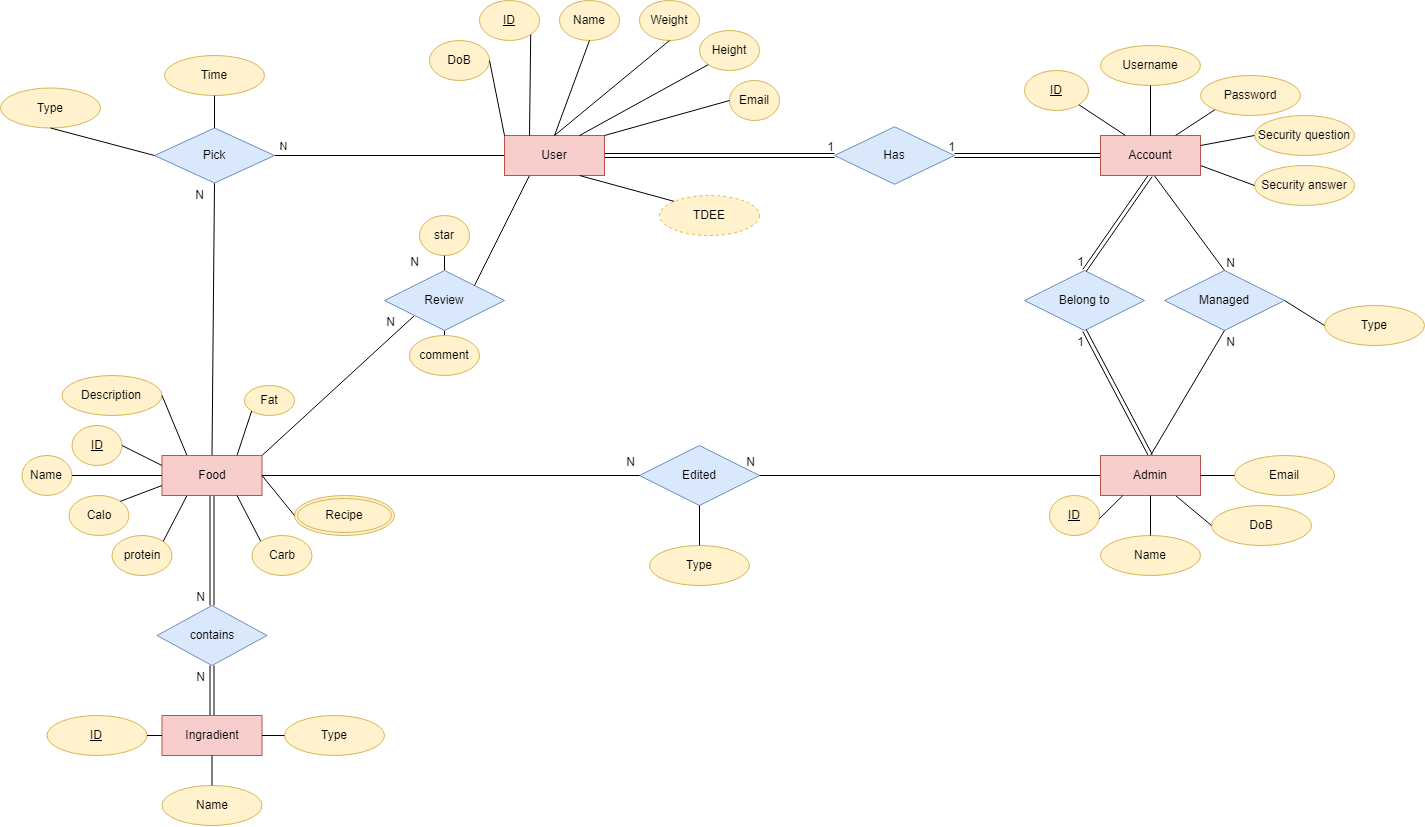
\includegraphics[width=0.99\linewidth]{images/backendDB/Foody_DB-ERD.drawio.png}
            \caption{ER Diagram of FOODY}
        \end{figure}
    \textbf{Link ảnh:} https://drive.google.com/file/d/1lA7-aU0gCllVa-p-Sp3iiUXmH4snUN0m/view?usp=sharing
    \newpage
    \subsection{Mapping}
        \begin{figure}[h]
            \centering
            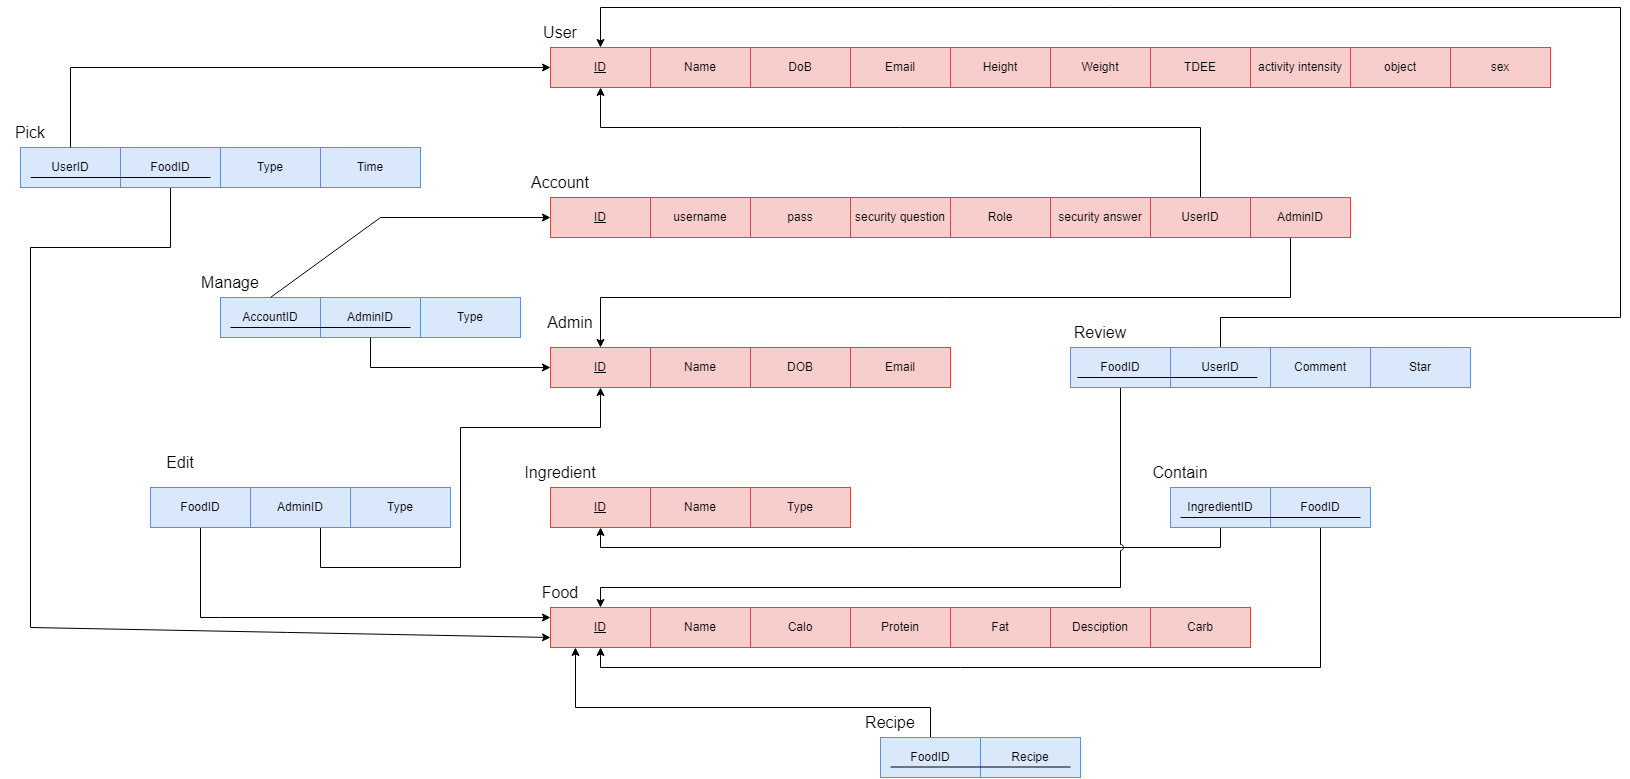
\includegraphics[width=0.99\linewidth]{images/backendDB/Foody_DB-Mapping.drawio.png}
            \caption{Mapping of FOODY}
        \end{figure}
        \textbf{Link ảnh:} https://drive.google.com/file/d/1NyA6kv1SKYCjilm013Aqxx2CA7a8xhSQ/view?usp=sharing
    \newpage
    \subsection{Tables in Mysql}
    Dựa vào thiết kết ý niệm và thiết kế luận lý ở ERD và Mapping ở trên, có thể hiện thực trong Mysql và có kết quả như sau:
        \begin{figure}[h]
            \centering
            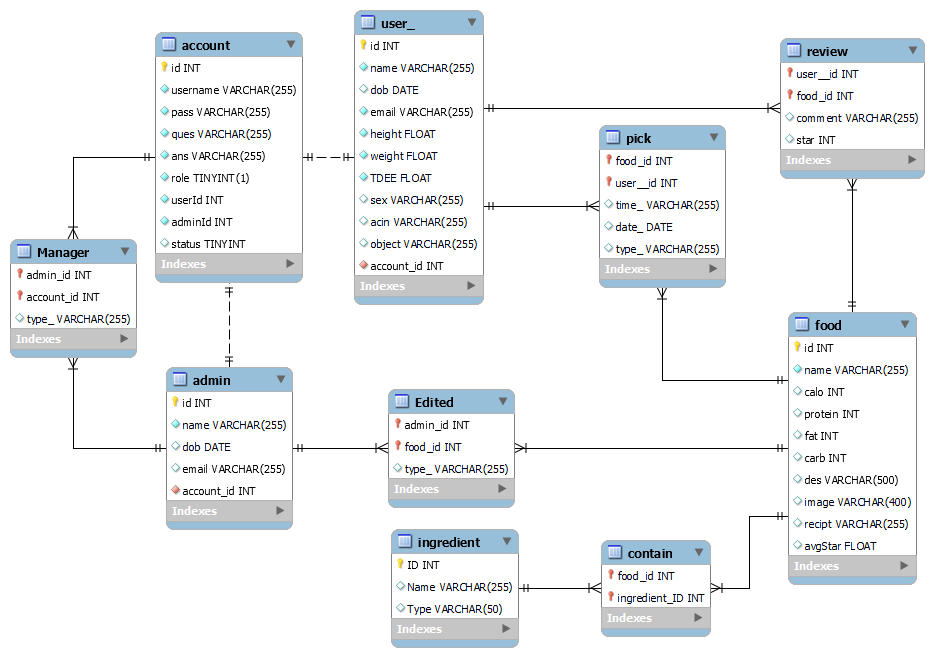
\includegraphics[width=0.99\linewidth]{images/backendDB/sqltable.png}
            \caption{In Mysql}
        \end{figure}
        \textbf{Link ảnh:} https://drive.google.com/file/d/1-6Bw8UxXbeNI\_D4qqNOI5LfYTKBnHXyI/view?usp=sharing
\documentclass[a4paper]{article}
\usepackage[english]{babel}
\usepackage[utf8]{vietnam}
\usepackage{a4wide,amssymb,epsfig,latexsym,multicol,array,hhline,fancyhdr}
\usepackage{amsmath}
\usepackage{lastpage}
\usepackage[lined,boxed,commentsnumbered]{algorithm2e}
\usepackage{enumerate}
\usepackage{color}
\usepackage{graphicx}							
% Standard graphics package
\usepackage{tabularx, caption}
\usepackage{tabularray}
\usepackage{longtable}
\usepackage{multirow}
\usepackage{rotating}
\usepackage{graphics}
\usepackage[a4paper,left=2cm,right=2cm,top=1.8cm,bottom=2.8cm]{geometry}
\usepackage{setspace}
\usepackage{tikz}
\usetikzlibrary{arrows,snakes,backgrounds}
\usepackage[unicode]{hyperref}

%can file puenc.def trong thu muc goc de option [unicode] tao ra bookmark bang tieng Viet
\hypersetup{urlcolor=blue,linkcolor=black,citecolor=black,colorlinks=true} 

\newtheorem{theorem}{{\bf Theorem}}
\newtheorem{property}{{\bf Property}}
\newtheorem{proposition}{{\bf Proposition}}
\newtheorem{corollary}[proposition]{{\bf Corollary}}
\newtheorem{lemma}[proposition]{{\bf Lemma}}

\newcommand\tab[1][0.5cm]{\hspace*{#1}}

\setlength{\headheight}{40pt}
\pagestyle{fancy}
\fancyhead{} % clear all header fields
\fancyhead[L]{
 \begin{tabular}{rl}
    \begin{picture}(25,15)(0,0)
    \put(0,-8){
\includegraphics[width=8mm, height=8mm]{images/hcmut.png}}
    %\put(0,-8){\epsfig{width=10mm,figure=hcmut.eps}}
   \end{picture}&
	%
\includegraphics[width=8mm, height=8mm]{hcmut.png} & %
	\begin{tabular}{l}
		\textbf{\bf \ttfamily Ho Chi Minh City University of Technology, VNU-HCM}\\
		\textbf{\bf \ttfamily Faculty of Computer Science \& Engineering}
	\end{tabular} 	
 \end{tabular}
}
\fancyhead[R]{
	\begin{tabular}{l}
		\tiny \bf \\
		\tiny \bf 
	\end{tabular}  }
\fancyfoot{} % clear all footer fields
\fancyfoot[L]{\scriptsize \ttfamily Đồ án tổng hợp- Hướng công nghệ phần mềm (CO3103), HK 221}
\fancyfoot[R]{\scriptsize \ttfamily Page {\thepage}/\pageref{LastPage}}
\renewcommand{\headrulewidth}{0.3pt}
\renewcommand{\footrulewidth}{0.3pt}


%%%
\setcounter{secnumdepth}{4}
\setcounter{tocdepth}{3}
\makeatletter
\newcounter {subsubsubsection}[subsubsection]
\renewcommand\thesubsubsubsection{\thesubsubsection .\@alph\c@subsubsubsection}
\newcommand\subsubsubsection{\@startsection{subsubsubsection}{4}{\z@}%
                                     {-3.25ex\@plus -1ex \@minus -.2ex}%
                                     {1.5ex \@plus .2ex}%
                                     {\normalfont\normalsize\bfseries}}
\newcommand*\l@subsubsubsection{\@dottedtocline{3}{10.0em}{4.1em}}
\newcommand*{\subsubsubsectionmark}[1]{}
\makeatother

\AtBeginDocument{\renewcommand*\contentsname{Nội dung}}

\begin{document}

\input{sections/title}

\newpage
\tableofcontents

\include{sections/member}
\include{sections/requirement elicitation/main}
\include{sections/use-case diagram/main}
\include{sections/appropriate framework/main}
\include{sections/backendDB/backendDB}
\include{sections/mockup UI/main}
\include{sections/implementation/implementation}

% \inlcude{sections/reference}

\end{document}
\section{Hiện thực và đánh giá ứng dụng}
    \subsection{Yêu cầu phiên bản}
        \begin{enumerate}
            \item \textbf{Backend:}
            \begin{itemize}
                \item Python: v3.10.8
                \item mySQL: v8.0
            \end{itemize}

            \item \textbf{Frontend:}
            \begin{itemize}
                \item NodeJS: v18
                \item React Native: v0.69.6
                \item Expo: v46.0.16
            \end{itemize}

            \item \textbf{Thiết bị hỗ trợ:}
            \begin{itemize}
                \item Các thiết bị sử dụng hệ điều hành Android.
                \item Phiên bản hỗ trợ: Android 10 trở lên.
            \end{itemize}
        \end{enumerate}

    \subsection{Đánh giá ứng dụng}
        \subsubsection{Ưu điểm}
        \begin{enumerate}
            \item Giao diện trực quan, dễ nắm bắt và sử dụng.
            \item Hệ thống hoạt động ổn đinh.
            \item Cá nhân hóa lịch ăn của người dùng dựa trên thông số TDEE và mục tiêu cá nhân.
            \item Người dùng có thể đánh giá cũng như đưa ra những bình luận về món ăn.
            \item Người quản lý có thể quản lý và thực hiện ban những người dùng có những bình luận thiếu ý thức.
            \item Người quản lý có thể chỉnh sửa các món ăn có trong hệ thống.
        \end{enumerate}

        \subsubsection{Nhược điểm}
        \begin{itemize}
            \item Chưa có hướng dẫn từng bước nấu ăn, còn phụ thuộc vào video của bên thứ ba.
            \item Chưa cho phép upload ảnh và video.
            \item Chỉ mới hỗ trợ android, chưa hỗ trợ iOS.
            \item Thiết kế api backend chưa thật sự hiệu quả.
        \end{itemize}

% \inlcude{sections/reference}

\end{document}
\section{Hiện thực Database}
    \subsection{ER Diagram}
    Dựa vào Use-case Diagram kèm theo các mô tả cho từng use-case ở phần 2. Xác định được các thực thể và mối quan hệ cho Database như sau:
        \begin{itemize}
            \item Thực thể: \textbf{User}, \textbf{account}, \textbf{admin}, \textbf{food}, \textbf{ingredient}.
            \item Mối quan hệ: User-\textbf{review}-food, User-\textbf{pick}-food, food-\textbf{contain}-ingredient, admin-\textbf{edited}-food, account-\textbf{belongto}-admin, admin-\textbf{manage}-account.
        \end{itemize}
        \begin{figure}[h]
            \centering
            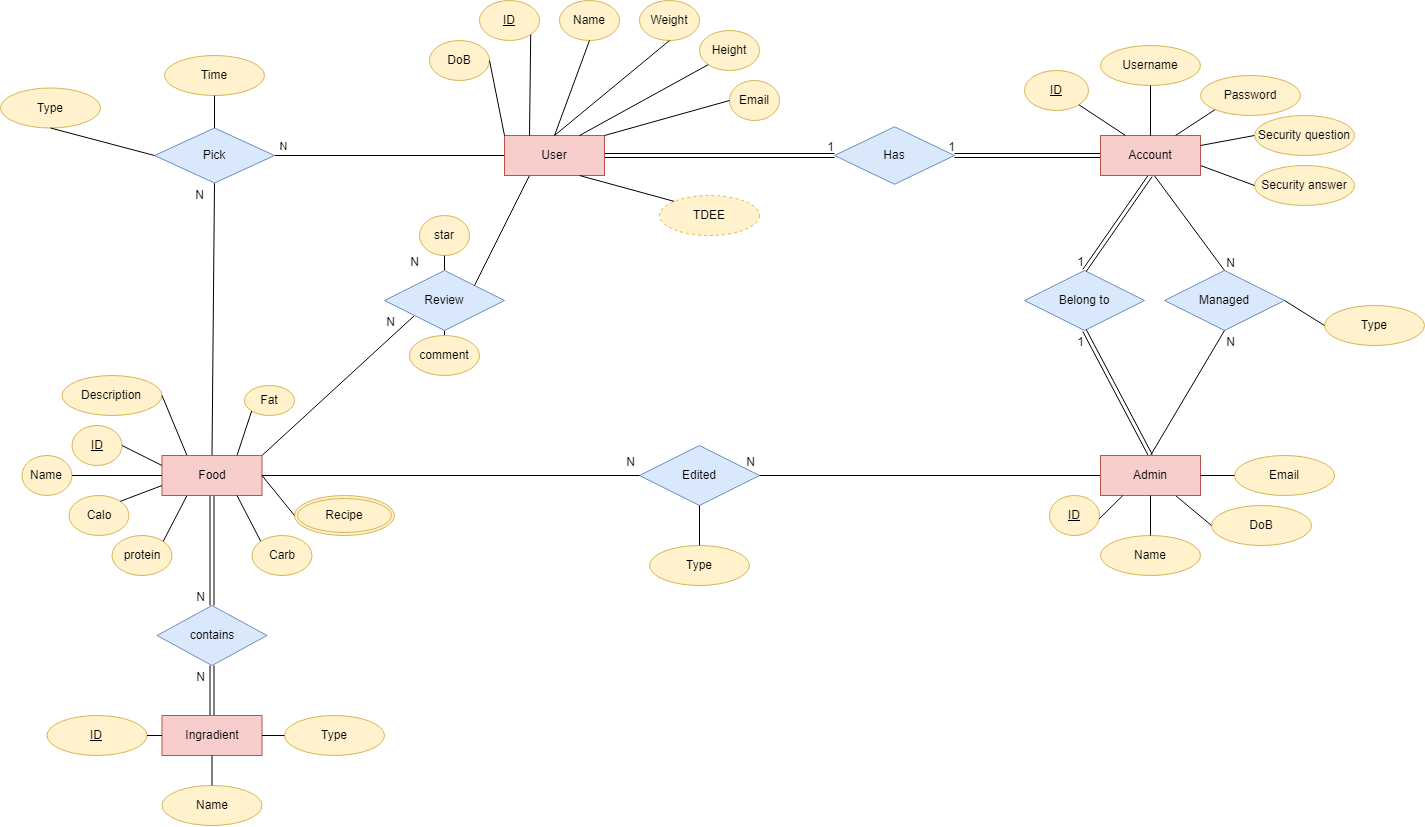
\includegraphics[width=0.99\linewidth]{images/backendDB/Foody_DB-ERD.drawio.png}
            \caption{ER Diagram of FOODY}
        \end{figure}
    \textbf{Link ảnh:} https://drive.google.com/file/d/1lA7-aU0gCllVa-p-Sp3iiUXmH4snUN0m/view?usp=sharing
    \newpage
    \subsection{Mapping}
        \begin{figure}[h]
            \centering
            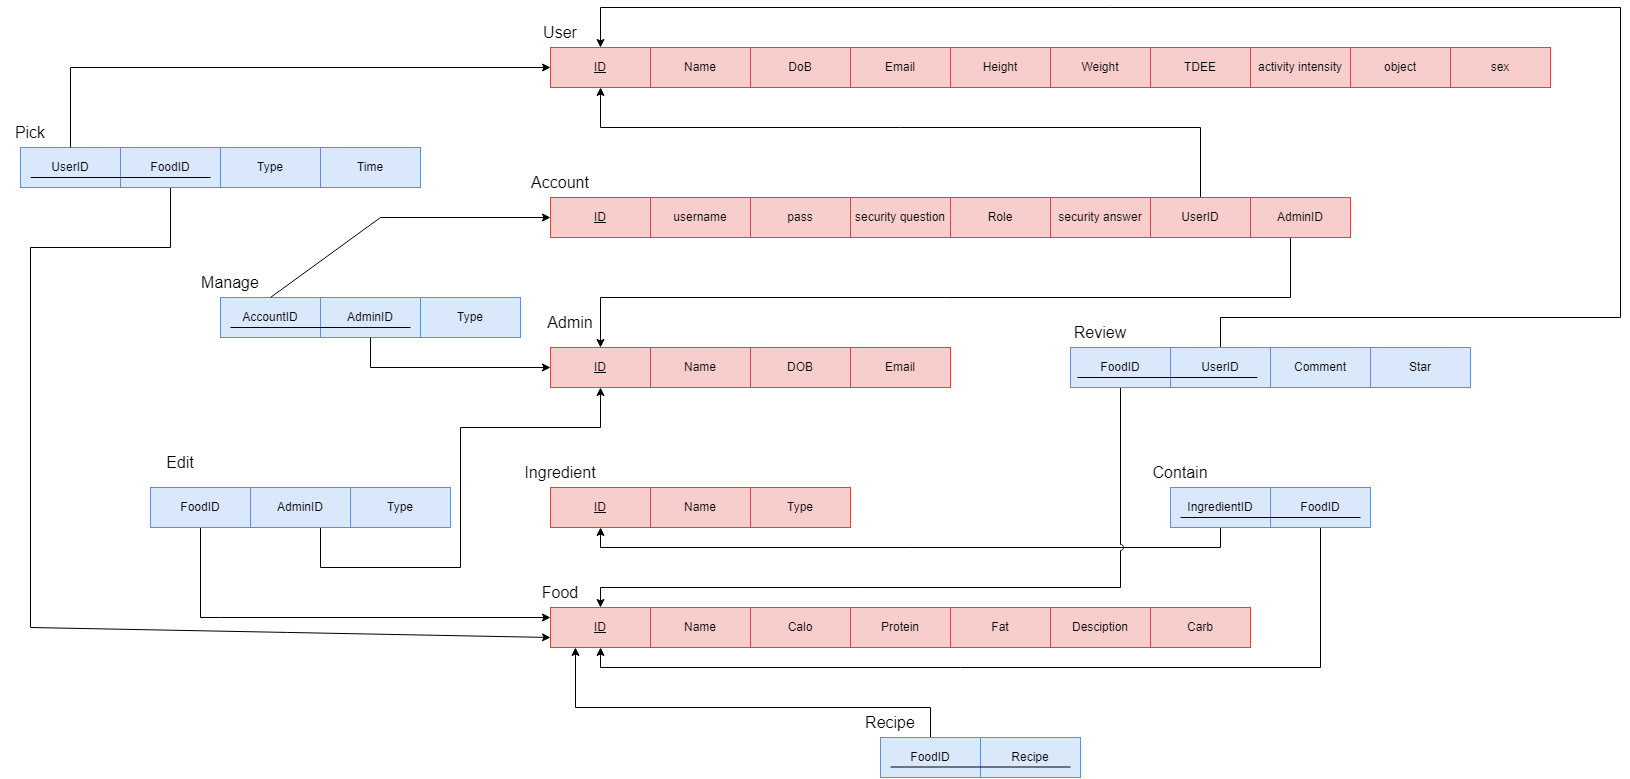
\includegraphics[width=0.99\linewidth]{images/backendDB/Foody_DB-Mapping.drawio.png}
            \caption{Mapping of FOODY}
        \end{figure}
        \textbf{Link ảnh:} https://drive.google.com/file/d/1NyA6kv1SKYCjilm013Aqxx2CA7a8xhSQ/view?usp=sharing
    \newpage
    \subsection{Tables in Mysql}
    Dựa vào thiết kết ý niệm và thiết kế luận lý ở ERD và Mapping ở trên, có thể hiện thực trong Mysql và có kết quả như sau:
        \begin{figure}[h]
            \centering
            \includegraphics[width=0.99\linewidth]{images/backendDB/sqltable.png}
            \caption{In Mysql}
        \end{figure}
        \textbf{Link ảnh:} https://drive.google.com/file/d/1-6Bw8UxXbeNI\_D4qqNOI5LfYTKBnHXyI/view?usp=sharing
\documentclass[a4paper]{article}
\usepackage[english]{babel}
\usepackage[utf8]{vietnam}
\usepackage{a4wide,amssymb,epsfig,latexsym,multicol,array,hhline,fancyhdr}
\usepackage{amsmath}
\usepackage{lastpage}
\usepackage[lined,boxed,commentsnumbered]{algorithm2e}
\usepackage{enumerate}
\usepackage{color}
\usepackage{graphicx}							
% Standard graphics package
\usepackage{tabularx, caption}
\usepackage{tabularray}
\usepackage{longtable}
\usepackage{multirow}
\usepackage{rotating}
\usepackage{graphics}
\usepackage[a4paper,left=2cm,right=2cm,top=1.8cm,bottom=2.8cm]{geometry}
\usepackage{setspace}
\usepackage{tikz}
\usetikzlibrary{arrows,snakes,backgrounds}
\usepackage[unicode]{hyperref}

%can file puenc.def trong thu muc goc de option [unicode] tao ra bookmark bang tieng Viet
\hypersetup{urlcolor=blue,linkcolor=black,citecolor=black,colorlinks=true} 

\newtheorem{theorem}{{\bf Theorem}}
\newtheorem{property}{{\bf Property}}
\newtheorem{proposition}{{\bf Proposition}}
\newtheorem{corollary}[proposition]{{\bf Corollary}}
\newtheorem{lemma}[proposition]{{\bf Lemma}}

\newcommand\tab[1][0.5cm]{\hspace*{#1}}

\setlength{\headheight}{40pt}
\pagestyle{fancy}
\fancyhead{} % clear all header fields
\fancyhead[L]{
 \begin{tabular}{rl}
    \begin{picture}(25,15)(0,0)
    \put(0,-8){\includegraphics[width=8mm, height=8mm]{images/hcmut.png}}
    %\put(0,-8){\epsfig{width=10mm,figure=hcmut.eps}}
   \end{picture}&
	%\includegraphics[width=8mm, height=8mm]{hcmut.png} & %
	\begin{tabular}{l}
		\textbf{\bf \ttfamily Ho Chi Minh City University of Technology, VNU-HCM}\\
		\textbf{\bf \ttfamily Faculty of Computer Science \& Engineering}
	\end{tabular} 	
 \end{tabular}
}
\fancyhead[R]{
	\begin{tabular}{l}
		\tiny \bf \\
		\tiny \bf 
	\end{tabular}  }
\fancyfoot{} % clear all footer fields
\fancyfoot[L]{\scriptsize \ttfamily Đồ án tổng hợp- Hướng công nghệ phần mềm (CO3103), HK 221}
\fancyfoot[R]{\scriptsize \ttfamily Page {\thepage}/\pageref{LastPage}}
\renewcommand{\headrulewidth}{0.3pt}
\renewcommand{\footrulewidth}{0.3pt}


%%%
\setcounter{secnumdepth}{4}
\setcounter{tocdepth}{3}
\makeatletter
\newcounter {subsubsubsection}[subsubsection]
\renewcommand\thesubsubsubsection{\thesubsubsection .\@alph\c@subsubsubsection}
\newcommand\subsubsubsection{\@startsection{subsubsubsection}{4}{\z@}%
                                     {-3.25ex\@plus -1ex \@minus -.2ex}%
                                     {1.5ex \@plus .2ex}%
                                     {\normalfont\normalsize\bfseries}}
\newcommand*\l@subsubsubsection{\@dottedtocline{3}{10.0em}{4.1em}}
\newcommand*{\subsubsubsectionmark}[1]{}
\makeatother

\AtBeginDocument{\renewcommand*\contentsname{Nội dung}}

\begin{document}


\graphicspath{{\subfix{../images/}}}
\begin{titlepage}

\begin{center}
    \large
    ĐẠI HỌC QUỐC GIA THÀNH PHỐ HỒ CHÍ MINH \\
    TRƯỜNG ĐẠI HỌC BÁCH KHOA \\
    KHOA KHOA HỌC VÀ KỸ THUẬT MÁY TÍNH \\
\end{center}

\vspace{1cm}

\begin{figure}[h!]
\begin{center}
\includegraphics[width=3cm]{images/hcmut.png}
\end{center}
\end{figure}

\vspace{1cm}


\begin{center}
\begin{tabular}{c}
\multicolumn{1}{l}{\textbf{{\Large ĐỒ ÁN TỔNG HỢP- HƯỚNG CÔNG NGHỆ PHẦN MỀM}}}\\
~~\\
\hline
\\
\multicolumn{1}{l}{\textbf{{\Large Report}}}\\
\\
\textbf{\Large ỨNG DỤNG ĐỀ XUẤT MÓN ĂN} \\ \textbf{\Large PHÙ HỢP VỚI NGƯỜI DÙNG (FOODY)}\\
\\
\hline
\end{tabular}
\end{center}

\vspace{3cm}

\begin{table}[h]
\begin{tabular}{rrl}

\hspace{5 cm} & GVHD: &\textbf{Lê Đình Thuận} \\
& & \textbf{Mai Đức Trung} \\
& Lớp: &L01 \\
& Thành viên: & - Lê Nguyễn Huyền Thoại - 2012122 \textbf{(Nhóm trưởng)} \\
& &  - Lê Văn Bằng - 2012684\\
& &  - Nguyễn Ngọc Hùng - 2013368 \\
& &  - Lê Trí Nguyên - 2013913 \\
& &  - Trần Văn Kiên - 2013552 \\

\end{tabular}
\end{table}

\vspace{4cm}
\begin{center}
{\footnotesize Hồ Chí Minh, 09/2022}
\end{center}
\end{titlepage}

\newpage
\tableofcontents

\section{Danh sách thành viên \& Khối lượng công việc}

\begin{tblr}{
    width=1\linewidth,
    hlines,
    vlines,
    colspec={X[-2]X[4]X[1.5]X[6]X[-1]},
    columns = {valign = m, },
    column{1} = {halign = c, },
    row{1} = {halign = c, valign = m, bg = lightgray, fg = black},
}
    {\textbf{STT} & \textbf{Họ và tên} & \textbf{MSSV} & \textbf{Công việc} & \textbf{Hoàn thành} }  \\
    1 & Lê Nguyễn Huyền Thoại & 2012122 & - Quản lý tiến độ công việc \newline
                                          - Thiểt kế use-case diagram gợi ý món ăn \newline
                                          - Thiết kế UI \newline
                                          - Hiện thực phần user view front end
                                        & 100\% \\
    2 & Lê Văn Bằng           & 2012684 & - Xác định yêu cầu phi chức năng \newline
                                          - Viết mô tả cho use-case diagram \newline
                                          - Hiện thực phần authentication front end
                                        & 100\% \\
    3 & Nguyễn Ngọc Hùng	  & 2013368 & - Xác định yêu cầu chức năng \newline
                                          - Thiết kế use-case xác thực \newline
                                          - Thiết kế database \newline
                                          - Hiện thực backend \newline
                                        & 100\% \\
    4 & Lê Trí Nguyên         & 2013913 & - Thiết kế use-case diagram tổng \newline
                                          - Thiết kế database \newline
                                          - Hiện thực backend \newline
                                        & 100\% \\
    5 & Trần Văn Kiên         & 2013552 & - Xác định ngữ cảnh và yêu cầu phi chức năng \newline
                                          - Tìm hiểu công nghệ \newline
                                          - Hiện thực phần admin-view front end
                                        & 100\% \\

\end{tblr}

\documentclass[a4paper]{article}
\usepackage[english]{babel}
\usepackage[utf8]{vietnam}
\usepackage{a4wide,amssymb,epsfig,latexsym,multicol,array,hhline,fancyhdr}
\usepackage{amsmath}
\usepackage{lastpage}
\usepackage[lined,boxed,commentsnumbered]{algorithm2e}
\usepackage{enumerate}
\usepackage{color}
\usepackage{graphicx}							
% Standard graphics package
\usepackage{tabularx, caption}
\usepackage{tabularray}
\usepackage{longtable}
\usepackage{multirow}
\usepackage{rotating}
\usepackage{graphics}
\usepackage[a4paper,left=2cm,right=2cm,top=1.8cm,bottom=2.8cm]{geometry}
\usepackage{setspace}
\usepackage{tikz}
\usetikzlibrary{arrows,snakes,backgrounds}
\usepackage[unicode]{hyperref}

%can file puenc.def trong thu muc goc de option [unicode] tao ra bookmark bang tieng Viet
\hypersetup{urlcolor=blue,linkcolor=black,citecolor=black,colorlinks=true} 

\newtheorem{theorem}{{\bf Theorem}}
\newtheorem{property}{{\bf Property}}
\newtheorem{proposition}{{\bf Proposition}}
\newtheorem{corollary}[proposition]{{\bf Corollary}}
\newtheorem{lemma}[proposition]{{\bf Lemma}}

\newcommand\tab[1][0.5cm]{\hspace*{#1}}

\setlength{\headheight}{40pt}
\pagestyle{fancy}
\fancyhead{} % clear all header fields
\fancyhead[L]{
 \begin{tabular}{rl}
    \begin{picture}(25,15)(0,0)
    \put(0,-8){\includegraphics[width=8mm, height=8mm]{images/hcmut.png}}
    %\put(0,-8){\epsfig{width=10mm,figure=hcmut.eps}}
   \end{picture}&
	%\includegraphics[width=8mm, height=8mm]{hcmut.png} & %
	\begin{tabular}{l}
		\textbf{\bf \ttfamily Ho Chi Minh City University of Technology, VNU-HCM}\\
		\textbf{\bf \ttfamily Faculty of Computer Science \& Engineering}
	\end{tabular} 	
 \end{tabular}
}
\fancyhead[R]{
	\begin{tabular}{l}
		\tiny \bf \\
		\tiny \bf 
	\end{tabular}  }
\fancyfoot{} % clear all footer fields
\fancyfoot[L]{\scriptsize \ttfamily Đồ án tổng hợp- Hướng công nghệ phần mềm (CO3103), HK 221}
\fancyfoot[R]{\scriptsize \ttfamily Page {\thepage}/\pageref{LastPage}}
\renewcommand{\headrulewidth}{0.3pt}
\renewcommand{\footrulewidth}{0.3pt}


%%%
\setcounter{secnumdepth}{4}
\setcounter{tocdepth}{3}
\makeatletter
\newcounter {subsubsubsection}[subsubsection]
\renewcommand\thesubsubsubsection{\thesubsubsection .\@alph\c@subsubsubsection}
\newcommand\subsubsubsection{\@startsection{subsubsubsection}{4}{\z@}%
                                     {-3.25ex\@plus -1ex \@minus -.2ex}%
                                     {1.5ex \@plus .2ex}%
                                     {\normalfont\normalsize\bfseries}}
\newcommand*\l@subsubsubsection{\@dottedtocline{3}{10.0em}{4.1em}}
\newcommand*{\subsubsubsectionmark}[1]{}
\makeatother

\AtBeginDocument{\renewcommand*\contentsname{Nội dung}}

\begin{document}

\input{sections/title}

\newpage
\tableofcontents

\include{sections/member}
\include{sections/requirement elicitation/main}
\include{sections/use-case diagram/main}
\include{sections/appropriate framework/main}
\include{sections/backendDB/backendDB}
\include{sections/mockup UI/main}
\include{sections/implementation/implementation}

% \inlcude{sections/reference}

\end{document}
\documentclass[a4paper]{article}
\usepackage[english]{babel}
\usepackage[utf8]{vietnam}
\usepackage{a4wide,amssymb,epsfig,latexsym,multicol,array,hhline,fancyhdr}
\usepackage{amsmath}
\usepackage{lastpage}
\usepackage[lined,boxed,commentsnumbered]{algorithm2e}
\usepackage{enumerate}
\usepackage{color}
\usepackage{graphicx}							
% Standard graphics package
\usepackage{tabularx, caption}
\usepackage{tabularray}
\usepackage{longtable}
\usepackage{multirow}
\usepackage{rotating}
\usepackage{graphics}
\usepackage[a4paper,left=2cm,right=2cm,top=1.8cm,bottom=2.8cm]{geometry}
\usepackage{setspace}
\usepackage{tikz}
\usetikzlibrary{arrows,snakes,backgrounds}
\usepackage[unicode]{hyperref}

%can file puenc.def trong thu muc goc de option [unicode] tao ra bookmark bang tieng Viet
\hypersetup{urlcolor=blue,linkcolor=black,citecolor=black,colorlinks=true} 

\newtheorem{theorem}{{\bf Theorem}}
\newtheorem{property}{{\bf Property}}
\newtheorem{proposition}{{\bf Proposition}}
\newtheorem{corollary}[proposition]{{\bf Corollary}}
\newtheorem{lemma}[proposition]{{\bf Lemma}}

\newcommand\tab[1][0.5cm]{\hspace*{#1}}

\setlength{\headheight}{40pt}
\pagestyle{fancy}
\fancyhead{} % clear all header fields
\fancyhead[L]{
 \begin{tabular}{rl}
    \begin{picture}(25,15)(0,0)
    \put(0,-8){\includegraphics[width=8mm, height=8mm]{images/hcmut.png}}
    %\put(0,-8){\epsfig{width=10mm,figure=hcmut.eps}}
   \end{picture}&
	%\includegraphics[width=8mm, height=8mm]{hcmut.png} & %
	\begin{tabular}{l}
		\textbf{\bf \ttfamily Ho Chi Minh City University of Technology, VNU-HCM}\\
		\textbf{\bf \ttfamily Faculty of Computer Science \& Engineering}
	\end{tabular} 	
 \end{tabular}
}
\fancyhead[R]{
	\begin{tabular}{l}
		\tiny \bf \\
		\tiny \bf 
	\end{tabular}  }
\fancyfoot{} % clear all footer fields
\fancyfoot[L]{\scriptsize \ttfamily Đồ án tổng hợp- Hướng công nghệ phần mềm (CO3103), HK 221}
\fancyfoot[R]{\scriptsize \ttfamily Page {\thepage}/\pageref{LastPage}}
\renewcommand{\headrulewidth}{0.3pt}
\renewcommand{\footrulewidth}{0.3pt}


%%%
\setcounter{secnumdepth}{4}
\setcounter{tocdepth}{3}
\makeatletter
\newcounter {subsubsubsection}[subsubsection]
\renewcommand\thesubsubsubsection{\thesubsubsection .\@alph\c@subsubsubsection}
\newcommand\subsubsubsection{\@startsection{subsubsubsection}{4}{\z@}%
                                     {-3.25ex\@plus -1ex \@minus -.2ex}%
                                     {1.5ex \@plus .2ex}%
                                     {\normalfont\normalsize\bfseries}}
\newcommand*\l@subsubsubsection{\@dottedtocline{3}{10.0em}{4.1em}}
\newcommand*{\subsubsubsectionmark}[1]{}
\makeatother

\AtBeginDocument{\renewcommand*\contentsname{Nội dung}}

\begin{document}

\input{sections/title}

\newpage
\tableofcontents

\include{sections/member}
\include{sections/requirement elicitation/main}
\include{sections/use-case diagram/main}
\include{sections/appropriate framework/main}
\include{sections/backendDB/backendDB}
\include{sections/mockup UI/main}
\include{sections/implementation/implementation}

% \inlcude{sections/reference}

\end{document}
\documentclass[a4paper]{article}
\usepackage[english]{babel}
\usepackage[utf8]{vietnam}
\usepackage{a4wide,amssymb,epsfig,latexsym,multicol,array,hhline,fancyhdr}
\usepackage{amsmath}
\usepackage{lastpage}
\usepackage[lined,boxed,commentsnumbered]{algorithm2e}
\usepackage{enumerate}
\usepackage{color}
\usepackage{graphicx}							
% Standard graphics package
\usepackage{tabularx, caption}
\usepackage{tabularray}
\usepackage{longtable}
\usepackage{multirow}
\usepackage{rotating}
\usepackage{graphics}
\usepackage[a4paper,left=2cm,right=2cm,top=1.8cm,bottom=2.8cm]{geometry}
\usepackage{setspace}
\usepackage{tikz}
\usetikzlibrary{arrows,snakes,backgrounds}
\usepackage[unicode]{hyperref}

%can file puenc.def trong thu muc goc de option [unicode] tao ra bookmark bang tieng Viet
\hypersetup{urlcolor=blue,linkcolor=black,citecolor=black,colorlinks=true} 

\newtheorem{theorem}{{\bf Theorem}}
\newtheorem{property}{{\bf Property}}
\newtheorem{proposition}{{\bf Proposition}}
\newtheorem{corollary}[proposition]{{\bf Corollary}}
\newtheorem{lemma}[proposition]{{\bf Lemma}}

\newcommand\tab[1][0.5cm]{\hspace*{#1}}

\setlength{\headheight}{40pt}
\pagestyle{fancy}
\fancyhead{} % clear all header fields
\fancyhead[L]{
 \begin{tabular}{rl}
    \begin{picture}(25,15)(0,0)
    \put(0,-8){\includegraphics[width=8mm, height=8mm]{images/hcmut.png}}
    %\put(0,-8){\epsfig{width=10mm,figure=hcmut.eps}}
   \end{picture}&
	%\includegraphics[width=8mm, height=8mm]{hcmut.png} & %
	\begin{tabular}{l}
		\textbf{\bf \ttfamily Ho Chi Minh City University of Technology, VNU-HCM}\\
		\textbf{\bf \ttfamily Faculty of Computer Science \& Engineering}
	\end{tabular} 	
 \end{tabular}
}
\fancyhead[R]{
	\begin{tabular}{l}
		\tiny \bf \\
		\tiny \bf 
	\end{tabular}  }
\fancyfoot{} % clear all footer fields
\fancyfoot[L]{\scriptsize \ttfamily Đồ án tổng hợp- Hướng công nghệ phần mềm (CO3103), HK 221}
\fancyfoot[R]{\scriptsize \ttfamily Page {\thepage}/\pageref{LastPage}}
\renewcommand{\headrulewidth}{0.3pt}
\renewcommand{\footrulewidth}{0.3pt}


%%%
\setcounter{secnumdepth}{4}
\setcounter{tocdepth}{3}
\makeatletter
\newcounter {subsubsubsection}[subsubsection]
\renewcommand\thesubsubsubsection{\thesubsubsection .\@alph\c@subsubsubsection}
\newcommand\subsubsubsection{\@startsection{subsubsubsection}{4}{\z@}%
                                     {-3.25ex\@plus -1ex \@minus -.2ex}%
                                     {1.5ex \@plus .2ex}%
                                     {\normalfont\normalsize\bfseries}}
\newcommand*\l@subsubsubsection{\@dottedtocline{3}{10.0em}{4.1em}}
\newcommand*{\subsubsubsectionmark}[1]{}
\makeatother

\AtBeginDocument{\renewcommand*\contentsname{Nội dung}}

\begin{document}

\input{sections/title}

\newpage
\tableofcontents

\include{sections/member}
\include{sections/requirement elicitation/main}
\include{sections/use-case diagram/main}
\include{sections/appropriate framework/main}
\include{sections/backendDB/backendDB}
\include{sections/mockup UI/main}
\include{sections/implementation/implementation}

% \inlcude{sections/reference}

\end{document}
\section{Hiện thực Database}
    \subsection{ER Diagram}
    Dựa vào Use-case Diagram kèm theo các mô tả cho từng use-case ở phần 2. Xác định được các thực thể và mối quan hệ cho Database như sau:
        \begin{itemize}
            \item Thực thể: \textbf{User}, \textbf{account}, \textbf{admin}, \textbf{food}, \textbf{ingredient}.
            \item Mối quan hệ: User-\textbf{review}-food, User-\textbf{pick}-food, food-\textbf{contain}-ingredient, admin-\textbf{edited}-food, account-\textbf{belongto}-admin, admin-\textbf{manage}-account.
        \end{itemize}
        \begin{figure}[h]
            \centering
            \includegraphics[width=0.99\linewidth]{images/backendDB/Foody_DB-ERD.drawio.png}
            \caption{ER Diagram of FOODY}
        \end{figure}
    \textbf{Link ảnh:} https://drive.google.com/file/d/1lA7-aU0gCllVa-p-Sp3iiUXmH4snUN0m/view?usp=sharing
    \newpage
    \subsection{Mapping}
        \begin{figure}[h]
            \centering
            \includegraphics[width=0.99\linewidth]{images/backendDB/Foody_DB-Mapping.drawio.png}
            \caption{Mapping of FOODY}
        \end{figure}
        \textbf{Link ảnh:} https://drive.google.com/file/d/1NyA6kv1SKYCjilm013Aqxx2CA7a8xhSQ/view?usp=sharing
    \newpage
    \subsection{Tables in Mysql}
    Dựa vào thiết kết ý niệm và thiết kế luận lý ở ERD và Mapping ở trên, có thể hiện thực trong Mysql và có kết quả như sau:
        \begin{figure}[h]
            \centering
            \includegraphics[width=0.99\linewidth]{images/backendDB/sqltable.png}
            \caption{In Mysql}
        \end{figure}
        \textbf{Link ảnh:} https://drive.google.com/file/d/1-6Bw8UxXbeNI\_D4qqNOI5LfYTKBnHXyI/view?usp=sharing
\documentclass[a4paper]{article}
\usepackage[english]{babel}
\usepackage[utf8]{vietnam}
\usepackage{a4wide,amssymb,epsfig,latexsym,multicol,array,hhline,fancyhdr}
\usepackage{amsmath}
\usepackage{lastpage}
\usepackage[lined,boxed,commentsnumbered]{algorithm2e}
\usepackage{enumerate}
\usepackage{color}
\usepackage{graphicx}							
% Standard graphics package
\usepackage{tabularx, caption}
\usepackage{tabularray}
\usepackage{longtable}
\usepackage{multirow}
\usepackage{rotating}
\usepackage{graphics}
\usepackage[a4paper,left=2cm,right=2cm,top=1.8cm,bottom=2.8cm]{geometry}
\usepackage{setspace}
\usepackage{tikz}
\usetikzlibrary{arrows,snakes,backgrounds}
\usepackage[unicode]{hyperref}

%can file puenc.def trong thu muc goc de option [unicode] tao ra bookmark bang tieng Viet
\hypersetup{urlcolor=blue,linkcolor=black,citecolor=black,colorlinks=true} 

\newtheorem{theorem}{{\bf Theorem}}
\newtheorem{property}{{\bf Property}}
\newtheorem{proposition}{{\bf Proposition}}
\newtheorem{corollary}[proposition]{{\bf Corollary}}
\newtheorem{lemma}[proposition]{{\bf Lemma}}

\newcommand\tab[1][0.5cm]{\hspace*{#1}}

\setlength{\headheight}{40pt}
\pagestyle{fancy}
\fancyhead{} % clear all header fields
\fancyhead[L]{
 \begin{tabular}{rl}
    \begin{picture}(25,15)(0,0)
    \put(0,-8){\includegraphics[width=8mm, height=8mm]{images/hcmut.png}}
    %\put(0,-8){\epsfig{width=10mm,figure=hcmut.eps}}
   \end{picture}&
	%\includegraphics[width=8mm, height=8mm]{hcmut.png} & %
	\begin{tabular}{l}
		\textbf{\bf \ttfamily Ho Chi Minh City University of Technology, VNU-HCM}\\
		\textbf{\bf \ttfamily Faculty of Computer Science \& Engineering}
	\end{tabular} 	
 \end{tabular}
}
\fancyhead[R]{
	\begin{tabular}{l}
		\tiny \bf \\
		\tiny \bf 
	\end{tabular}  }
\fancyfoot{} % clear all footer fields
\fancyfoot[L]{\scriptsize \ttfamily Đồ án tổng hợp- Hướng công nghệ phần mềm (CO3103), HK 221}
\fancyfoot[R]{\scriptsize \ttfamily Page {\thepage}/\pageref{LastPage}}
\renewcommand{\headrulewidth}{0.3pt}
\renewcommand{\footrulewidth}{0.3pt}


%%%
\setcounter{secnumdepth}{4}
\setcounter{tocdepth}{3}
\makeatletter
\newcounter {subsubsubsection}[subsubsection]
\renewcommand\thesubsubsubsection{\thesubsubsection .\@alph\c@subsubsubsection}
\newcommand\subsubsubsection{\@startsection{subsubsubsection}{4}{\z@}%
                                     {-3.25ex\@plus -1ex \@minus -.2ex}%
                                     {1.5ex \@plus .2ex}%
                                     {\normalfont\normalsize\bfseries}}
\newcommand*\l@subsubsubsection{\@dottedtocline{3}{10.0em}{4.1em}}
\newcommand*{\subsubsubsectionmark}[1]{}
\makeatother

\AtBeginDocument{\renewcommand*\contentsname{Nội dung}}

\begin{document}

\input{sections/title}

\newpage
\tableofcontents

\include{sections/member}
\include{sections/requirement elicitation/main}
\include{sections/use-case diagram/main}
\include{sections/appropriate framework/main}
\include{sections/backendDB/backendDB}
\include{sections/mockup UI/main}
\include{sections/implementation/implementation}

% \inlcude{sections/reference}

\end{document}
\section{Hiện thực và đánh giá ứng dụng}
    \subsection{Yêu cầu phiên bản}
        \begin{enumerate}
            \item \textbf{Backend:}
            \begin{itemize}
                \item Python: v3.10.8
                \item mySQL: v8.0
            \end{itemize}

            \item \textbf{Frontend:}
            \begin{itemize}
                \item NodeJS: v18
                \item React Native: v0.69.6
                \item Expo: v46.0.16
            \end{itemize}

            \item \textbf{Thiết bị hỗ trợ:}
            \begin{itemize}
                \item Các thiết bị sử dụng hệ điều hành Android.
                \item Phiên bản hỗ trợ: Android 10 trở lên.
            \end{itemize}
        \end{enumerate}

    \subsection{Đánh giá ứng dụng}
        \subsubsection{Ưu điểm}
        \begin{enumerate}
            \item Giao diện trực quan, dễ nắm bắt và sử dụng.
            \item Hệ thống hoạt động ổn đinh.
            \item Cá nhân hóa lịch ăn của người dùng dựa trên thông số TDEE và mục tiêu cá nhân.
            \item Người dùng có thể đánh giá cũng như đưa ra những bình luận về món ăn.
            \item Người quản lý có thể quản lý và thực hiện ban những người dùng có những bình luận thiếu ý thức.
            \item Người quản lý có thể chỉnh sửa các món ăn có trong hệ thống.
        \end{enumerate}

        \subsubsection{Nhược điểm}
        \begin{itemize}
            \item Chưa có hướng dẫn từng bước nấu ăn, còn phụ thuộc vào video của bên thứ ba.
            \item Chưa cho phép upload ảnh và video.
            \item Chỉ mới hỗ trợ android, chưa hỗ trợ iOS.
            \item Thiết kế api backend chưa thật sự hiệu quả.
        \end{itemize}

% \inlcude{sections/reference}

\end{document}
\section{Hiện thực và đánh giá ứng dụng}
    \subsection{Yêu cầu phiên bản}
        \begin{enumerate}
            \item \textbf{Backend:}
            \begin{itemize}
                \item Python: v3.10.8
                \item mySQL: v8.0
            \end{itemize}

            \item \textbf{Frontend:}
            \begin{itemize}
                \item NodeJS: v18
                \item React Native: v0.69.6
                \item Expo: v46.0.16
            \end{itemize}

            \item \textbf{Thiết bị hỗ trợ:}
            \begin{itemize}
                \item Các thiết bị sử dụng hệ điều hành Android.
                \item Phiên bản hỗ trợ: Android 10 trở lên.
            \end{itemize}
        \end{enumerate}

    \subsection{Đánh giá ứng dụng}
        \subsubsection{Ưu điểm}
        \begin{enumerate}
            \item Giao diện trực quan, dễ nắm bắt và sử dụng.
            \item Hệ thống hoạt động ổn đinh.
            \item Cá nhân hóa lịch ăn của người dùng dựa trên thông số TDEE và mục tiêu cá nhân.
            \item Người dùng có thể đánh giá cũng như đưa ra những bình luận về món ăn.
            \item Người quản lý có thể quản lý và thực hiện ban những người dùng có những bình luận thiếu ý thức.
            \item Người quản lý có thể chỉnh sửa các món ăn có trong hệ thống.
        \end{enumerate}

        \subsubsection{Nhược điểm}
        \begin{itemize}
            \item Chưa có hướng dẫn từng bước nấu ăn, còn phụ thuộc vào video của bên thứ ba.
            \item Chưa cho phép upload ảnh và video.
            \item Chỉ mới hỗ trợ android, chưa hỗ trợ iOS.
            \item Thiết kế api backend chưa thật sự hiệu quả.
        \end{itemize}

% \inlcude{sections/reference}

\end{document}
\documentclass[a4paper]{article}
\usepackage[english]{babel}
\usepackage[utf8]{vietnam}
\usepackage{a4wide,amssymb,epsfig,latexsym,multicol,array,hhline,fancyhdr}
\usepackage{amsmath}
\usepackage{lastpage}
\usepackage[lined,boxed,commentsnumbered]{algorithm2e}
\usepackage{enumerate}
\usepackage{color}
\usepackage{graphicx}							
% Standard graphics package
\usepackage{tabularx, caption}
\usepackage{tabularray}
\usepackage{longtable}
\usepackage{multirow}
\usepackage{rotating}
\usepackage{graphics}
\usepackage[a4paper,left=2cm,right=2cm,top=1.8cm,bottom=2.8cm]{geometry}
\usepackage{setspace}
\usepackage{tikz}
\usetikzlibrary{arrows,snakes,backgrounds}
\usepackage[unicode]{hyperref}

%can file puenc.def trong thu muc goc de option [unicode] tao ra bookmark bang tieng Viet
\hypersetup{urlcolor=blue,linkcolor=black,citecolor=black,colorlinks=true} 

\newtheorem{theorem}{{\bf Theorem}}
\newtheorem{property}{{\bf Property}}
\newtheorem{proposition}{{\bf Proposition}}
\newtheorem{corollary}[proposition]{{\bf Corollary}}
\newtheorem{lemma}[proposition]{{\bf Lemma}}

\newcommand\tab[1][0.5cm]{\hspace*{#1}}

\setlength{\headheight}{40pt}
\pagestyle{fancy}
\fancyhead{} % clear all header fields
\fancyhead[L]{
 \begin{tabular}{rl}
    \begin{picture}(25,15)(0,0)
    \put(0,-8){\includegraphics[width=8mm, height=8mm]{images/hcmut.png}}
    %\put(0,-8){\epsfig{width=10mm,figure=hcmut.eps}}
   \end{picture}&
	%\includegraphics[width=8mm, height=8mm]{hcmut.png} & %
	\begin{tabular}{l}
		\textbf{\bf \ttfamily Ho Chi Minh City University of Technology, VNU-HCM}\\
		\textbf{\bf \ttfamily Faculty of Computer Science \& Engineering}
	\end{tabular} 	
 \end{tabular}
}
\fancyhead[R]{
	\begin{tabular}{l}
		\tiny \bf \\
		\tiny \bf 
	\end{tabular}  }
\fancyfoot{} % clear all footer fields
\fancyfoot[L]{\scriptsize \ttfamily Đồ án tổng hợp- Hướng công nghệ phần mềm (CO3103), HK 221}
\fancyfoot[R]{\scriptsize \ttfamily Page {\thepage}/\pageref{LastPage}}
\renewcommand{\headrulewidth}{0.3pt}
\renewcommand{\footrulewidth}{0.3pt}


%%%
\setcounter{secnumdepth}{4}
\setcounter{tocdepth}{3}
\makeatletter
\newcounter {subsubsubsection}[subsubsection]
\renewcommand\thesubsubsubsection{\thesubsubsection .\@alph\c@subsubsubsection}
\newcommand\subsubsubsection{\@startsection{subsubsubsection}{4}{\z@}%
                                     {-3.25ex\@plus -1ex \@minus -.2ex}%
                                     {1.5ex \@plus .2ex}%
                                     {\normalfont\normalsize\bfseries}}
\newcommand*\l@subsubsubsection{\@dottedtocline{3}{10.0em}{4.1em}}
\newcommand*{\subsubsubsectionmark}[1]{}
\makeatother

\AtBeginDocument{\renewcommand*\contentsname{Nội dung}}

\begin{document}


\graphicspath{{\subfix{../images/}}}
\begin{titlepage}

\begin{center}
    \large
    ĐẠI HỌC QUỐC GIA THÀNH PHỐ HỒ CHÍ MINH \\
    TRƯỜNG ĐẠI HỌC BÁCH KHOA \\
    KHOA KHOA HỌC VÀ KỸ THUẬT MÁY TÍNH \\
\end{center}

\vspace{1cm}

\begin{figure}[h!]
\begin{center}
\includegraphics[width=3cm]{images/hcmut.png}
\end{center}
\end{figure}

\vspace{1cm}


\begin{center}
\begin{tabular}{c}
\multicolumn{1}{l}{\textbf{{\Large ĐỒ ÁN TỔNG HỢP- HƯỚNG CÔNG NGHỆ PHẦN MỀM}}}\\
~~\\
\hline
\\
\multicolumn{1}{l}{\textbf{{\Large Report}}}\\
\\
\textbf{\Large ỨNG DỤNG ĐỀ XUẤT MÓN ĂN} \\ \textbf{\Large PHÙ HỢP VỚI NGƯỜI DÙNG (FOODY)}\\
\\
\hline
\end{tabular}
\end{center}

\vspace{3cm}

\begin{table}[h]
\begin{tabular}{rrl}

\hspace{5 cm} & GVHD: &\textbf{Lê Đình Thuận} \\
& & \textbf{Mai Đức Trung} \\
& Lớp: &L01 \\
& Thành viên: & - Lê Nguyễn Huyền Thoại - 2012122 \textbf{(Nhóm trưởng)} \\
& &  - Lê Văn Bằng - 2012684\\
& &  - Nguyễn Ngọc Hùng - 2013368 \\
& &  - Lê Trí Nguyên - 2013913 \\
& &  - Trần Văn Kiên - 2013552 \\

\end{tabular}
\end{table}

\vspace{4cm}
\begin{center}
{\footnotesize Hồ Chí Minh, 09/2022}
\end{center}
\end{titlepage}

\newpage
\tableofcontents

\section{Danh sách thành viên \& Khối lượng công việc}

\begin{tblr}{
    width=1\linewidth,
    hlines,
    vlines,
    colspec={X[-2]X[4]X[1.5]X[6]X[-1]},
    columns = {valign = m, },
    column{1} = {halign = c, },
    row{1} = {halign = c, valign = m, bg = lightgray, fg = black},
}
    {\textbf{STT} & \textbf{Họ và tên} & \textbf{MSSV} & \textbf{Công việc} & \textbf{Hoàn thành} }  \\
    1 & Lê Nguyễn Huyền Thoại & 2012122 & - Quản lý tiến độ công việc \newline
                                          - Thiểt kế use-case diagram gợi ý món ăn \newline
                                          - Thiết kế UI \newline
                                          - Hiện thực phần user view front end
                                        & 100\% \\
    2 & Lê Văn Bằng           & 2012684 & - Xác định yêu cầu phi chức năng \newline
                                          - Viết mô tả cho use-case diagram \newline
                                          - Hiện thực phần authentication front end
                                        & 100\% \\
    3 & Nguyễn Ngọc Hùng	  & 2013368 & - Xác định yêu cầu chức năng \newline
                                          - Thiết kế use-case xác thực \newline
                                          - Thiết kế database \newline
                                          - Hiện thực backend \newline
                                        & 100\% \\
    4 & Lê Trí Nguyên         & 2013913 & - Thiết kế use-case diagram tổng \newline
                                          - Thiết kế database \newline
                                          - Hiện thực backend \newline
                                        & 100\% \\
    5 & Trần Văn Kiên         & 2013552 & - Xác định ngữ cảnh và yêu cầu phi chức năng \newline
                                          - Tìm hiểu công nghệ \newline
                                          - Hiện thực phần admin-view front end
                                        & 100\% \\

\end{tblr}

\documentclass[a4paper]{article}
\usepackage[english]{babel}
\usepackage[utf8]{vietnam}
\usepackage{a4wide,amssymb,epsfig,latexsym,multicol,array,hhline,fancyhdr}
\usepackage{amsmath}
\usepackage{lastpage}
\usepackage[lined,boxed,commentsnumbered]{algorithm2e}
\usepackage{enumerate}
\usepackage{color}
\usepackage{graphicx}							
% Standard graphics package
\usepackage{tabularx, caption}
\usepackage{tabularray}
\usepackage{longtable}
\usepackage{multirow}
\usepackage{rotating}
\usepackage{graphics}
\usepackage[a4paper,left=2cm,right=2cm,top=1.8cm,bottom=2.8cm]{geometry}
\usepackage{setspace}
\usepackage{tikz}
\usetikzlibrary{arrows,snakes,backgrounds}
\usepackage[unicode]{hyperref}

%can file puenc.def trong thu muc goc de option [unicode] tao ra bookmark bang tieng Viet
\hypersetup{urlcolor=blue,linkcolor=black,citecolor=black,colorlinks=true} 

\newtheorem{theorem}{{\bf Theorem}}
\newtheorem{property}{{\bf Property}}
\newtheorem{proposition}{{\bf Proposition}}
\newtheorem{corollary}[proposition]{{\bf Corollary}}
\newtheorem{lemma}[proposition]{{\bf Lemma}}

\newcommand\tab[1][0.5cm]{\hspace*{#1}}

\setlength{\headheight}{40pt}
\pagestyle{fancy}
\fancyhead{} % clear all header fields
\fancyhead[L]{
 \begin{tabular}{rl}
    \begin{picture}(25,15)(0,0)
    \put(0,-8){\includegraphics[width=8mm, height=8mm]{images/hcmut.png}}
    %\put(0,-8){\epsfig{width=10mm,figure=hcmut.eps}}
   \end{picture}&
	%\includegraphics[width=8mm, height=8mm]{hcmut.png} & %
	\begin{tabular}{l}
		\textbf{\bf \ttfamily Ho Chi Minh City University of Technology, VNU-HCM}\\
		\textbf{\bf \ttfamily Faculty of Computer Science \& Engineering}
	\end{tabular} 	
 \end{tabular}
}
\fancyhead[R]{
	\begin{tabular}{l}
		\tiny \bf \\
		\tiny \bf 
	\end{tabular}  }
\fancyfoot{} % clear all footer fields
\fancyfoot[L]{\scriptsize \ttfamily Đồ án tổng hợp- Hướng công nghệ phần mềm (CO3103), HK 221}
\fancyfoot[R]{\scriptsize \ttfamily Page {\thepage}/\pageref{LastPage}}
\renewcommand{\headrulewidth}{0.3pt}
\renewcommand{\footrulewidth}{0.3pt}


%%%
\setcounter{secnumdepth}{4}
\setcounter{tocdepth}{3}
\makeatletter
\newcounter {subsubsubsection}[subsubsection]
\renewcommand\thesubsubsubsection{\thesubsubsection .\@alph\c@subsubsubsection}
\newcommand\subsubsubsection{\@startsection{subsubsubsection}{4}{\z@}%
                                     {-3.25ex\@plus -1ex \@minus -.2ex}%
                                     {1.5ex \@plus .2ex}%
                                     {\normalfont\normalsize\bfseries}}
\newcommand*\l@subsubsubsection{\@dottedtocline{3}{10.0em}{4.1em}}
\newcommand*{\subsubsubsectionmark}[1]{}
\makeatother

\AtBeginDocument{\renewcommand*\contentsname{Nội dung}}

\begin{document}


\graphicspath{{\subfix{../images/}}}
\begin{titlepage}

\begin{center}
    \large
    ĐẠI HỌC QUỐC GIA THÀNH PHỐ HỒ CHÍ MINH \\
    TRƯỜNG ĐẠI HỌC BÁCH KHOA \\
    KHOA KHOA HỌC VÀ KỸ THUẬT MÁY TÍNH \\
\end{center}

\vspace{1cm}

\begin{figure}[h!]
\begin{center}
\includegraphics[width=3cm]{images/hcmut.png}
\end{center}
\end{figure}

\vspace{1cm}


\begin{center}
\begin{tabular}{c}
\multicolumn{1}{l}{\textbf{{\Large ĐỒ ÁN TỔNG HỢP- HƯỚNG CÔNG NGHỆ PHẦN MỀM}}}\\
~~\\
\hline
\\
\multicolumn{1}{l}{\textbf{{\Large Report}}}\\
\\
\textbf{\Large ỨNG DỤNG ĐỀ XUẤT MÓN ĂN} \\ \textbf{\Large PHÙ HỢP VỚI NGƯỜI DÙNG (FOODY)}\\
\\
\hline
\end{tabular}
\end{center}

\vspace{3cm}

\begin{table}[h]
\begin{tabular}{rrl}

\hspace{5 cm} & GVHD: &\textbf{Lê Đình Thuận} \\
& & \textbf{Mai Đức Trung} \\
& Lớp: &L01 \\
& Thành viên: & - Lê Nguyễn Huyền Thoại - 2012122 \textbf{(Nhóm trưởng)} \\
& &  - Lê Văn Bằng - 2012684\\
& &  - Nguyễn Ngọc Hùng - 2013368 \\
& &  - Lê Trí Nguyên - 2013913 \\
& &  - Trần Văn Kiên - 2013552 \\

\end{tabular}
\end{table}

\vspace{4cm}
\begin{center}
{\footnotesize Hồ Chí Minh, 09/2022}
\end{center}
\end{titlepage}

\newpage
\tableofcontents

\section{Danh sách thành viên \& Khối lượng công việc}

\begin{tblr}{
    width=1\linewidth,
    hlines,
    vlines,
    colspec={X[-2]X[4]X[1.5]X[6]X[-1]},
    columns = {valign = m, },
    column{1} = {halign = c, },
    row{1} = {halign = c, valign = m, bg = lightgray, fg = black},
}
    {\textbf{STT} & \textbf{Họ và tên} & \textbf{MSSV} & \textbf{Công việc} & \textbf{Hoàn thành} }  \\
    1 & Lê Nguyễn Huyền Thoại & 2012122 & - Quản lý tiến độ công việc \newline
                                          - Thiểt kế use-case diagram gợi ý món ăn \newline
                                          - Thiết kế UI \newline
                                          - Hiện thực phần user view front end
                                        & 100\% \\
    2 & Lê Văn Bằng           & 2012684 & - Xác định yêu cầu phi chức năng \newline
                                          - Viết mô tả cho use-case diagram \newline
                                          - Hiện thực phần authentication front end
                                        & 100\% \\
    3 & Nguyễn Ngọc Hùng	  & 2013368 & - Xác định yêu cầu chức năng \newline
                                          - Thiết kế use-case xác thực \newline
                                          - Thiết kế database \newline
                                          - Hiện thực backend \newline
                                        & 100\% \\
    4 & Lê Trí Nguyên         & 2013913 & - Thiết kế use-case diagram tổng \newline
                                          - Thiết kế database \newline
                                          - Hiện thực backend \newline
                                        & 100\% \\
    5 & Trần Văn Kiên         & 2013552 & - Xác định ngữ cảnh và yêu cầu phi chức năng \newline
                                          - Tìm hiểu công nghệ \newline
                                          - Hiện thực phần admin-view front end
                                        & 100\% \\

\end{tblr}

\documentclass[a4paper]{article}
\usepackage[english]{babel}
\usepackage[utf8]{vietnam}
\usepackage{a4wide,amssymb,epsfig,latexsym,multicol,array,hhline,fancyhdr}
\usepackage{amsmath}
\usepackage{lastpage}
\usepackage[lined,boxed,commentsnumbered]{algorithm2e}
\usepackage{enumerate}
\usepackage{color}
\usepackage{graphicx}							
% Standard graphics package
\usepackage{tabularx, caption}
\usepackage{tabularray}
\usepackage{longtable}
\usepackage{multirow}
\usepackage{rotating}
\usepackage{graphics}
\usepackage[a4paper,left=2cm,right=2cm,top=1.8cm,bottom=2.8cm]{geometry}
\usepackage{setspace}
\usepackage{tikz}
\usetikzlibrary{arrows,snakes,backgrounds}
\usepackage[unicode]{hyperref}

%can file puenc.def trong thu muc goc de option [unicode] tao ra bookmark bang tieng Viet
\hypersetup{urlcolor=blue,linkcolor=black,citecolor=black,colorlinks=true} 

\newtheorem{theorem}{{\bf Theorem}}
\newtheorem{property}{{\bf Property}}
\newtheorem{proposition}{{\bf Proposition}}
\newtheorem{corollary}[proposition]{{\bf Corollary}}
\newtheorem{lemma}[proposition]{{\bf Lemma}}

\newcommand\tab[1][0.5cm]{\hspace*{#1}}

\setlength{\headheight}{40pt}
\pagestyle{fancy}
\fancyhead{} % clear all header fields
\fancyhead[L]{
 \begin{tabular}{rl}
    \begin{picture}(25,15)(0,0)
    \put(0,-8){\includegraphics[width=8mm, height=8mm]{images/hcmut.png}}
    %\put(0,-8){\epsfig{width=10mm,figure=hcmut.eps}}
   \end{picture}&
	%\includegraphics[width=8mm, height=8mm]{hcmut.png} & %
	\begin{tabular}{l}
		\textbf{\bf \ttfamily Ho Chi Minh City University of Technology, VNU-HCM}\\
		\textbf{\bf \ttfamily Faculty of Computer Science \& Engineering}
	\end{tabular} 	
 \end{tabular}
}
\fancyhead[R]{
	\begin{tabular}{l}
		\tiny \bf \\
		\tiny \bf 
	\end{tabular}  }
\fancyfoot{} % clear all footer fields
\fancyfoot[L]{\scriptsize \ttfamily Đồ án tổng hợp- Hướng công nghệ phần mềm (CO3103), HK 221}
\fancyfoot[R]{\scriptsize \ttfamily Page {\thepage}/\pageref{LastPage}}
\renewcommand{\headrulewidth}{0.3pt}
\renewcommand{\footrulewidth}{0.3pt}


%%%
\setcounter{secnumdepth}{4}
\setcounter{tocdepth}{3}
\makeatletter
\newcounter {subsubsubsection}[subsubsection]
\renewcommand\thesubsubsubsection{\thesubsubsection .\@alph\c@subsubsubsection}
\newcommand\subsubsubsection{\@startsection{subsubsubsection}{4}{\z@}%
                                     {-3.25ex\@plus -1ex \@minus -.2ex}%
                                     {1.5ex \@plus .2ex}%
                                     {\normalfont\normalsize\bfseries}}
\newcommand*\l@subsubsubsection{\@dottedtocline{3}{10.0em}{4.1em}}
\newcommand*{\subsubsubsectionmark}[1]{}
\makeatother

\AtBeginDocument{\renewcommand*\contentsname{Nội dung}}

\begin{document}

\input{sections/title}

\newpage
\tableofcontents

\include{sections/member}
\include{sections/requirement elicitation/main}
\include{sections/use-case diagram/main}
\include{sections/appropriate framework/main}
\include{sections/backendDB/backendDB}
\include{sections/mockup UI/main}
\include{sections/implementation/implementation}

% \inlcude{sections/reference}

\end{document}
\documentclass[a4paper]{article}
\usepackage[english]{babel}
\usepackage[utf8]{vietnam}
\usepackage{a4wide,amssymb,epsfig,latexsym,multicol,array,hhline,fancyhdr}
\usepackage{amsmath}
\usepackage{lastpage}
\usepackage[lined,boxed,commentsnumbered]{algorithm2e}
\usepackage{enumerate}
\usepackage{color}
\usepackage{graphicx}							
% Standard graphics package
\usepackage{tabularx, caption}
\usepackage{tabularray}
\usepackage{longtable}
\usepackage{multirow}
\usepackage{rotating}
\usepackage{graphics}
\usepackage[a4paper,left=2cm,right=2cm,top=1.8cm,bottom=2.8cm]{geometry}
\usepackage{setspace}
\usepackage{tikz}
\usetikzlibrary{arrows,snakes,backgrounds}
\usepackage[unicode]{hyperref}

%can file puenc.def trong thu muc goc de option [unicode] tao ra bookmark bang tieng Viet
\hypersetup{urlcolor=blue,linkcolor=black,citecolor=black,colorlinks=true} 

\newtheorem{theorem}{{\bf Theorem}}
\newtheorem{property}{{\bf Property}}
\newtheorem{proposition}{{\bf Proposition}}
\newtheorem{corollary}[proposition]{{\bf Corollary}}
\newtheorem{lemma}[proposition]{{\bf Lemma}}

\newcommand\tab[1][0.5cm]{\hspace*{#1}}

\setlength{\headheight}{40pt}
\pagestyle{fancy}
\fancyhead{} % clear all header fields
\fancyhead[L]{
 \begin{tabular}{rl}
    \begin{picture}(25,15)(0,0)
    \put(0,-8){\includegraphics[width=8mm, height=8mm]{images/hcmut.png}}
    %\put(0,-8){\epsfig{width=10mm,figure=hcmut.eps}}
   \end{picture}&
	%\includegraphics[width=8mm, height=8mm]{hcmut.png} & %
	\begin{tabular}{l}
		\textbf{\bf \ttfamily Ho Chi Minh City University of Technology, VNU-HCM}\\
		\textbf{\bf \ttfamily Faculty of Computer Science \& Engineering}
	\end{tabular} 	
 \end{tabular}
}
\fancyhead[R]{
	\begin{tabular}{l}
		\tiny \bf \\
		\tiny \bf 
	\end{tabular}  }
\fancyfoot{} % clear all footer fields
\fancyfoot[L]{\scriptsize \ttfamily Đồ án tổng hợp- Hướng công nghệ phần mềm (CO3103), HK 221}
\fancyfoot[R]{\scriptsize \ttfamily Page {\thepage}/\pageref{LastPage}}
\renewcommand{\headrulewidth}{0.3pt}
\renewcommand{\footrulewidth}{0.3pt}


%%%
\setcounter{secnumdepth}{4}
\setcounter{tocdepth}{3}
\makeatletter
\newcounter {subsubsubsection}[subsubsection]
\renewcommand\thesubsubsubsection{\thesubsubsection .\@alph\c@subsubsubsection}
\newcommand\subsubsubsection{\@startsection{subsubsubsection}{4}{\z@}%
                                     {-3.25ex\@plus -1ex \@minus -.2ex}%
                                     {1.5ex \@plus .2ex}%
                                     {\normalfont\normalsize\bfseries}}
\newcommand*\l@subsubsubsection{\@dottedtocline{3}{10.0em}{4.1em}}
\newcommand*{\subsubsubsectionmark}[1]{}
\makeatother

\AtBeginDocument{\renewcommand*\contentsname{Nội dung}}

\begin{document}

\input{sections/title}

\newpage
\tableofcontents

\include{sections/member}
\include{sections/requirement elicitation/main}
\include{sections/use-case diagram/main}
\include{sections/appropriate framework/main}
\include{sections/backendDB/backendDB}
\include{sections/mockup UI/main}
\include{sections/implementation/implementation}

% \inlcude{sections/reference}

\end{document}
\documentclass[a4paper]{article}
\usepackage[english]{babel}
\usepackage[utf8]{vietnam}
\usepackage{a4wide,amssymb,epsfig,latexsym,multicol,array,hhline,fancyhdr}
\usepackage{amsmath}
\usepackage{lastpage}
\usepackage[lined,boxed,commentsnumbered]{algorithm2e}
\usepackage{enumerate}
\usepackage{color}
\usepackage{graphicx}							
% Standard graphics package
\usepackage{tabularx, caption}
\usepackage{tabularray}
\usepackage{longtable}
\usepackage{multirow}
\usepackage{rotating}
\usepackage{graphics}
\usepackage[a4paper,left=2cm,right=2cm,top=1.8cm,bottom=2.8cm]{geometry}
\usepackage{setspace}
\usepackage{tikz}
\usetikzlibrary{arrows,snakes,backgrounds}
\usepackage[unicode]{hyperref}

%can file puenc.def trong thu muc goc de option [unicode] tao ra bookmark bang tieng Viet
\hypersetup{urlcolor=blue,linkcolor=black,citecolor=black,colorlinks=true} 

\newtheorem{theorem}{{\bf Theorem}}
\newtheorem{property}{{\bf Property}}
\newtheorem{proposition}{{\bf Proposition}}
\newtheorem{corollary}[proposition]{{\bf Corollary}}
\newtheorem{lemma}[proposition]{{\bf Lemma}}

\newcommand\tab[1][0.5cm]{\hspace*{#1}}

\setlength{\headheight}{40pt}
\pagestyle{fancy}
\fancyhead{} % clear all header fields
\fancyhead[L]{
 \begin{tabular}{rl}
    \begin{picture}(25,15)(0,0)
    \put(0,-8){\includegraphics[width=8mm, height=8mm]{images/hcmut.png}}
    %\put(0,-8){\epsfig{width=10mm,figure=hcmut.eps}}
   \end{picture}&
	%\includegraphics[width=8mm, height=8mm]{hcmut.png} & %
	\begin{tabular}{l}
		\textbf{\bf \ttfamily Ho Chi Minh City University of Technology, VNU-HCM}\\
		\textbf{\bf \ttfamily Faculty of Computer Science \& Engineering}
	\end{tabular} 	
 \end{tabular}
}
\fancyhead[R]{
	\begin{tabular}{l}
		\tiny \bf \\
		\tiny \bf 
	\end{tabular}  }
\fancyfoot{} % clear all footer fields
\fancyfoot[L]{\scriptsize \ttfamily Đồ án tổng hợp- Hướng công nghệ phần mềm (CO3103), HK 221}
\fancyfoot[R]{\scriptsize \ttfamily Page {\thepage}/\pageref{LastPage}}
\renewcommand{\headrulewidth}{0.3pt}
\renewcommand{\footrulewidth}{0.3pt}


%%%
\setcounter{secnumdepth}{4}
\setcounter{tocdepth}{3}
\makeatletter
\newcounter {subsubsubsection}[subsubsection]
\renewcommand\thesubsubsubsection{\thesubsubsection .\@alph\c@subsubsubsection}
\newcommand\subsubsubsection{\@startsection{subsubsubsection}{4}{\z@}%
                                     {-3.25ex\@plus -1ex \@minus -.2ex}%
                                     {1.5ex \@plus .2ex}%
                                     {\normalfont\normalsize\bfseries}}
\newcommand*\l@subsubsubsection{\@dottedtocline{3}{10.0em}{4.1em}}
\newcommand*{\subsubsubsectionmark}[1]{}
\makeatother

\AtBeginDocument{\renewcommand*\contentsname{Nội dung}}

\begin{document}

\input{sections/title}

\newpage
\tableofcontents

\include{sections/member}
\include{sections/requirement elicitation/main}
\include{sections/use-case diagram/main}
\include{sections/appropriate framework/main}
\include{sections/backendDB/backendDB}
\include{sections/mockup UI/main}
\include{sections/implementation/implementation}

% \inlcude{sections/reference}

\end{document}
\section{Hiện thực Database}
    \subsection{ER Diagram}
    Dựa vào Use-case Diagram kèm theo các mô tả cho từng use-case ở phần 2. Xác định được các thực thể và mối quan hệ cho Database như sau:
        \begin{itemize}
            \item Thực thể: \textbf{User}, \textbf{account}, \textbf{admin}, \textbf{food}, \textbf{ingredient}.
            \item Mối quan hệ: User-\textbf{review}-food, User-\textbf{pick}-food, food-\textbf{contain}-ingredient, admin-\textbf{edited}-food, account-\textbf{belongto}-admin, admin-\textbf{manage}-account.
        \end{itemize}
        \begin{figure}[h]
            \centering
            \includegraphics[width=0.99\linewidth]{images/backendDB/Foody_DB-ERD.drawio.png}
            \caption{ER Diagram of FOODY}
        \end{figure}
    \textbf{Link ảnh:} https://drive.google.com/file/d/1lA7-aU0gCllVa-p-Sp3iiUXmH4snUN0m/view?usp=sharing
    \newpage
    \subsection{Mapping}
        \begin{figure}[h]
            \centering
            \includegraphics[width=0.99\linewidth]{images/backendDB/Foody_DB-Mapping.drawio.png}
            \caption{Mapping of FOODY}
        \end{figure}
        \textbf{Link ảnh:} https://drive.google.com/file/d/1NyA6kv1SKYCjilm013Aqxx2CA7a8xhSQ/view?usp=sharing
    \newpage
    \subsection{Tables in Mysql}
    Dựa vào thiết kết ý niệm và thiết kế luận lý ở ERD và Mapping ở trên, có thể hiện thực trong Mysql và có kết quả như sau:
        \begin{figure}[h]
            \centering
            \includegraphics[width=0.99\linewidth]{images/backendDB/sqltable.png}
            \caption{In Mysql}
        \end{figure}
        \textbf{Link ảnh:} https://drive.google.com/file/d/1-6Bw8UxXbeNI\_D4qqNOI5LfYTKBnHXyI/view?usp=sharing
\documentclass[a4paper]{article}
\usepackage[english]{babel}
\usepackage[utf8]{vietnam}
\usepackage{a4wide,amssymb,epsfig,latexsym,multicol,array,hhline,fancyhdr}
\usepackage{amsmath}
\usepackage{lastpage}
\usepackage[lined,boxed,commentsnumbered]{algorithm2e}
\usepackage{enumerate}
\usepackage{color}
\usepackage{graphicx}							
% Standard graphics package
\usepackage{tabularx, caption}
\usepackage{tabularray}
\usepackage{longtable}
\usepackage{multirow}
\usepackage{rotating}
\usepackage{graphics}
\usepackage[a4paper,left=2cm,right=2cm,top=1.8cm,bottom=2.8cm]{geometry}
\usepackage{setspace}
\usepackage{tikz}
\usetikzlibrary{arrows,snakes,backgrounds}
\usepackage[unicode]{hyperref}

%can file puenc.def trong thu muc goc de option [unicode] tao ra bookmark bang tieng Viet
\hypersetup{urlcolor=blue,linkcolor=black,citecolor=black,colorlinks=true} 

\newtheorem{theorem}{{\bf Theorem}}
\newtheorem{property}{{\bf Property}}
\newtheorem{proposition}{{\bf Proposition}}
\newtheorem{corollary}[proposition]{{\bf Corollary}}
\newtheorem{lemma}[proposition]{{\bf Lemma}}

\newcommand\tab[1][0.5cm]{\hspace*{#1}}

\setlength{\headheight}{40pt}
\pagestyle{fancy}
\fancyhead{} % clear all header fields
\fancyhead[L]{
 \begin{tabular}{rl}
    \begin{picture}(25,15)(0,0)
    \put(0,-8){\includegraphics[width=8mm, height=8mm]{images/hcmut.png}}
    %\put(0,-8){\epsfig{width=10mm,figure=hcmut.eps}}
   \end{picture}&
	%\includegraphics[width=8mm, height=8mm]{hcmut.png} & %
	\begin{tabular}{l}
		\textbf{\bf \ttfamily Ho Chi Minh City University of Technology, VNU-HCM}\\
		\textbf{\bf \ttfamily Faculty of Computer Science \& Engineering}
	\end{tabular} 	
 \end{tabular}
}
\fancyhead[R]{
	\begin{tabular}{l}
		\tiny \bf \\
		\tiny \bf 
	\end{tabular}  }
\fancyfoot{} % clear all footer fields
\fancyfoot[L]{\scriptsize \ttfamily Đồ án tổng hợp- Hướng công nghệ phần mềm (CO3103), HK 221}
\fancyfoot[R]{\scriptsize \ttfamily Page {\thepage}/\pageref{LastPage}}
\renewcommand{\headrulewidth}{0.3pt}
\renewcommand{\footrulewidth}{0.3pt}


%%%
\setcounter{secnumdepth}{4}
\setcounter{tocdepth}{3}
\makeatletter
\newcounter {subsubsubsection}[subsubsection]
\renewcommand\thesubsubsubsection{\thesubsubsection .\@alph\c@subsubsubsection}
\newcommand\subsubsubsection{\@startsection{subsubsubsection}{4}{\z@}%
                                     {-3.25ex\@plus -1ex \@minus -.2ex}%
                                     {1.5ex \@plus .2ex}%
                                     {\normalfont\normalsize\bfseries}}
\newcommand*\l@subsubsubsection{\@dottedtocline{3}{10.0em}{4.1em}}
\newcommand*{\subsubsubsectionmark}[1]{}
\makeatother

\AtBeginDocument{\renewcommand*\contentsname{Nội dung}}

\begin{document}

\input{sections/title}

\newpage
\tableofcontents

\include{sections/member}
\include{sections/requirement elicitation/main}
\include{sections/use-case diagram/main}
\include{sections/appropriate framework/main}
\include{sections/backendDB/backendDB}
\include{sections/mockup UI/main}
\include{sections/implementation/implementation}

% \inlcude{sections/reference}

\end{document}
\section{Hiện thực và đánh giá ứng dụng}
    \subsection{Yêu cầu phiên bản}
        \begin{enumerate}
            \item \textbf{Backend:}
            \begin{itemize}
                \item Python: v3.10.8
                \item mySQL: v8.0
            \end{itemize}

            \item \textbf{Frontend:}
            \begin{itemize}
                \item NodeJS: v18
                \item React Native: v0.69.6
                \item Expo: v46.0.16
            \end{itemize}

            \item \textbf{Thiết bị hỗ trợ:}
            \begin{itemize}
                \item Các thiết bị sử dụng hệ điều hành Android.
                \item Phiên bản hỗ trợ: Android 10 trở lên.
            \end{itemize}
        \end{enumerate}

    \subsection{Đánh giá ứng dụng}
        \subsubsection{Ưu điểm}
        \begin{enumerate}
            \item Giao diện trực quan, dễ nắm bắt và sử dụng.
            \item Hệ thống hoạt động ổn đinh.
            \item Cá nhân hóa lịch ăn của người dùng dựa trên thông số TDEE và mục tiêu cá nhân.
            \item Người dùng có thể đánh giá cũng như đưa ra những bình luận về món ăn.
            \item Người quản lý có thể quản lý và thực hiện ban những người dùng có những bình luận thiếu ý thức.
            \item Người quản lý có thể chỉnh sửa các món ăn có trong hệ thống.
        \end{enumerate}

        \subsubsection{Nhược điểm}
        \begin{itemize}
            \item Chưa có hướng dẫn từng bước nấu ăn, còn phụ thuộc vào video của bên thứ ba.
            \item Chưa cho phép upload ảnh và video.
            \item Chỉ mới hỗ trợ android, chưa hỗ trợ iOS.
            \item Thiết kế api backend chưa thật sự hiệu quả.
        \end{itemize}

% \inlcude{sections/reference}

\end{document}
\documentclass[a4paper]{article}
\usepackage[english]{babel}
\usepackage[utf8]{vietnam}
\usepackage{a4wide,amssymb,epsfig,latexsym,multicol,array,hhline,fancyhdr}
\usepackage{amsmath}
\usepackage{lastpage}
\usepackage[lined,boxed,commentsnumbered]{algorithm2e}
\usepackage{enumerate}
\usepackage{color}
\usepackage{graphicx}							
% Standard graphics package
\usepackage{tabularx, caption}
\usepackage{tabularray}
\usepackage{longtable}
\usepackage{multirow}
\usepackage{rotating}
\usepackage{graphics}
\usepackage[a4paper,left=2cm,right=2cm,top=1.8cm,bottom=2.8cm]{geometry}
\usepackage{setspace}
\usepackage{tikz}
\usetikzlibrary{arrows,snakes,backgrounds}
\usepackage[unicode]{hyperref}

%can file puenc.def trong thu muc goc de option [unicode] tao ra bookmark bang tieng Viet
\hypersetup{urlcolor=blue,linkcolor=black,citecolor=black,colorlinks=true} 

\newtheorem{theorem}{{\bf Theorem}}
\newtheorem{property}{{\bf Property}}
\newtheorem{proposition}{{\bf Proposition}}
\newtheorem{corollary}[proposition]{{\bf Corollary}}
\newtheorem{lemma}[proposition]{{\bf Lemma}}

\newcommand\tab[1][0.5cm]{\hspace*{#1}}

\setlength{\headheight}{40pt}
\pagestyle{fancy}
\fancyhead{} % clear all header fields
\fancyhead[L]{
 \begin{tabular}{rl}
    \begin{picture}(25,15)(0,0)
    \put(0,-8){\includegraphics[width=8mm, height=8mm]{images/hcmut.png}}
    %\put(0,-8){\epsfig{width=10mm,figure=hcmut.eps}}
   \end{picture}&
	%\includegraphics[width=8mm, height=8mm]{hcmut.png} & %
	\begin{tabular}{l}
		\textbf{\bf \ttfamily Ho Chi Minh City University of Technology, VNU-HCM}\\
		\textbf{\bf \ttfamily Faculty of Computer Science \& Engineering}
	\end{tabular} 	
 \end{tabular}
}
\fancyhead[R]{
	\begin{tabular}{l}
		\tiny \bf \\
		\tiny \bf 
	\end{tabular}  }
\fancyfoot{} % clear all footer fields
\fancyfoot[L]{\scriptsize \ttfamily Đồ án tổng hợp- Hướng công nghệ phần mềm (CO3103), HK 221}
\fancyfoot[R]{\scriptsize \ttfamily Page {\thepage}/\pageref{LastPage}}
\renewcommand{\headrulewidth}{0.3pt}
\renewcommand{\footrulewidth}{0.3pt}


%%%
\setcounter{secnumdepth}{4}
\setcounter{tocdepth}{3}
\makeatletter
\newcounter {subsubsubsection}[subsubsection]
\renewcommand\thesubsubsubsection{\thesubsubsection .\@alph\c@subsubsubsection}
\newcommand\subsubsubsection{\@startsection{subsubsubsection}{4}{\z@}%
                                     {-3.25ex\@plus -1ex \@minus -.2ex}%
                                     {1.5ex \@plus .2ex}%
                                     {\normalfont\normalsize\bfseries}}
\newcommand*\l@subsubsubsection{\@dottedtocline{3}{10.0em}{4.1em}}
\newcommand*{\subsubsubsectionmark}[1]{}
\makeatother

\AtBeginDocument{\renewcommand*\contentsname{Nội dung}}

\begin{document}


\graphicspath{{\subfix{../images/}}}
\begin{titlepage}

\begin{center}
    \large
    ĐẠI HỌC QUỐC GIA THÀNH PHỐ HỒ CHÍ MINH \\
    TRƯỜNG ĐẠI HỌC BÁCH KHOA \\
    KHOA KHOA HỌC VÀ KỸ THUẬT MÁY TÍNH \\
\end{center}

\vspace{1cm}

\begin{figure}[h!]
\begin{center}
\includegraphics[width=3cm]{images/hcmut.png}
\end{center}
\end{figure}

\vspace{1cm}


\begin{center}
\begin{tabular}{c}
\multicolumn{1}{l}{\textbf{{\Large ĐỒ ÁN TỔNG HỢP- HƯỚNG CÔNG NGHỆ PHẦN MỀM}}}\\
~~\\
\hline
\\
\multicolumn{1}{l}{\textbf{{\Large Report}}}\\
\\
\textbf{\Large ỨNG DỤNG ĐỀ XUẤT MÓN ĂN} \\ \textbf{\Large PHÙ HỢP VỚI NGƯỜI DÙNG (FOODY)}\\
\\
\hline
\end{tabular}
\end{center}

\vspace{3cm}

\begin{table}[h]
\begin{tabular}{rrl}

\hspace{5 cm} & GVHD: &\textbf{Lê Đình Thuận} \\
& & \textbf{Mai Đức Trung} \\
& Lớp: &L01 \\
& Thành viên: & - Lê Nguyễn Huyền Thoại - 2012122 \textbf{(Nhóm trưởng)} \\
& &  - Lê Văn Bằng - 2012684\\
& &  - Nguyễn Ngọc Hùng - 2013368 \\
& &  - Lê Trí Nguyên - 2013913 \\
& &  - Trần Văn Kiên - 2013552 \\

\end{tabular}
\end{table}

\vspace{4cm}
\begin{center}
{\footnotesize Hồ Chí Minh, 09/2022}
\end{center}
\end{titlepage}

\newpage
\tableofcontents

\section{Danh sách thành viên \& Khối lượng công việc}

\begin{tblr}{
    width=1\linewidth,
    hlines,
    vlines,
    colspec={X[-2]X[4]X[1.5]X[6]X[-1]},
    columns = {valign = m, },
    column{1} = {halign = c, },
    row{1} = {halign = c, valign = m, bg = lightgray, fg = black},
}
    {\textbf{STT} & \textbf{Họ và tên} & \textbf{MSSV} & \textbf{Công việc} & \textbf{Hoàn thành} }  \\
    1 & Lê Nguyễn Huyền Thoại & 2012122 & - Quản lý tiến độ công việc \newline
                                          - Thiểt kế use-case diagram gợi ý món ăn \newline
                                          - Thiết kế UI \newline
                                          - Hiện thực phần user view front end
                                        & 100\% \\
    2 & Lê Văn Bằng           & 2012684 & - Xác định yêu cầu phi chức năng \newline
                                          - Viết mô tả cho use-case diagram \newline
                                          - Hiện thực phần authentication front end
                                        & 100\% \\
    3 & Nguyễn Ngọc Hùng	  & 2013368 & - Xác định yêu cầu chức năng \newline
                                          - Thiết kế use-case xác thực \newline
                                          - Thiết kế database \newline
                                          - Hiện thực backend \newline
                                        & 100\% \\
    4 & Lê Trí Nguyên         & 2013913 & - Thiết kế use-case diagram tổng \newline
                                          - Thiết kế database \newline
                                          - Hiện thực backend \newline
                                        & 100\% \\
    5 & Trần Văn Kiên         & 2013552 & - Xác định ngữ cảnh và yêu cầu phi chức năng \newline
                                          - Tìm hiểu công nghệ \newline
                                          - Hiện thực phần admin-view front end
                                        & 100\% \\

\end{tblr}

\documentclass[a4paper]{article}
\usepackage[english]{babel}
\usepackage[utf8]{vietnam}
\usepackage{a4wide,amssymb,epsfig,latexsym,multicol,array,hhline,fancyhdr}
\usepackage{amsmath}
\usepackage{lastpage}
\usepackage[lined,boxed,commentsnumbered]{algorithm2e}
\usepackage{enumerate}
\usepackage{color}
\usepackage{graphicx}							
% Standard graphics package
\usepackage{tabularx, caption}
\usepackage{tabularray}
\usepackage{longtable}
\usepackage{multirow}
\usepackage{rotating}
\usepackage{graphics}
\usepackage[a4paper,left=2cm,right=2cm,top=1.8cm,bottom=2.8cm]{geometry}
\usepackage{setspace}
\usepackage{tikz}
\usetikzlibrary{arrows,snakes,backgrounds}
\usepackage[unicode]{hyperref}

%can file puenc.def trong thu muc goc de option [unicode] tao ra bookmark bang tieng Viet
\hypersetup{urlcolor=blue,linkcolor=black,citecolor=black,colorlinks=true} 

\newtheorem{theorem}{{\bf Theorem}}
\newtheorem{property}{{\bf Property}}
\newtheorem{proposition}{{\bf Proposition}}
\newtheorem{corollary}[proposition]{{\bf Corollary}}
\newtheorem{lemma}[proposition]{{\bf Lemma}}

\newcommand\tab[1][0.5cm]{\hspace*{#1}}

\setlength{\headheight}{40pt}
\pagestyle{fancy}
\fancyhead{} % clear all header fields
\fancyhead[L]{
 \begin{tabular}{rl}
    \begin{picture}(25,15)(0,0)
    \put(0,-8){\includegraphics[width=8mm, height=8mm]{images/hcmut.png}}
    %\put(0,-8){\epsfig{width=10mm,figure=hcmut.eps}}
   \end{picture}&
	%\includegraphics[width=8mm, height=8mm]{hcmut.png} & %
	\begin{tabular}{l}
		\textbf{\bf \ttfamily Ho Chi Minh City University of Technology, VNU-HCM}\\
		\textbf{\bf \ttfamily Faculty of Computer Science \& Engineering}
	\end{tabular} 	
 \end{tabular}
}
\fancyhead[R]{
	\begin{tabular}{l}
		\tiny \bf \\
		\tiny \bf 
	\end{tabular}  }
\fancyfoot{} % clear all footer fields
\fancyfoot[L]{\scriptsize \ttfamily Đồ án tổng hợp- Hướng công nghệ phần mềm (CO3103), HK 221}
\fancyfoot[R]{\scriptsize \ttfamily Page {\thepage}/\pageref{LastPage}}
\renewcommand{\headrulewidth}{0.3pt}
\renewcommand{\footrulewidth}{0.3pt}


%%%
\setcounter{secnumdepth}{4}
\setcounter{tocdepth}{3}
\makeatletter
\newcounter {subsubsubsection}[subsubsection]
\renewcommand\thesubsubsubsection{\thesubsubsection .\@alph\c@subsubsubsection}
\newcommand\subsubsubsection{\@startsection{subsubsubsection}{4}{\z@}%
                                     {-3.25ex\@plus -1ex \@minus -.2ex}%
                                     {1.5ex \@plus .2ex}%
                                     {\normalfont\normalsize\bfseries}}
\newcommand*\l@subsubsubsection{\@dottedtocline{3}{10.0em}{4.1em}}
\newcommand*{\subsubsubsectionmark}[1]{}
\makeatother

\AtBeginDocument{\renewcommand*\contentsname{Nội dung}}

\begin{document}

\input{sections/title}

\newpage
\tableofcontents

\include{sections/member}
\include{sections/requirement elicitation/main}
\include{sections/use-case diagram/main}
\include{sections/appropriate framework/main}
\include{sections/backendDB/backendDB}
\include{sections/mockup UI/main}
\include{sections/implementation/implementation}

% \inlcude{sections/reference}

\end{document}
\documentclass[a4paper]{article}
\usepackage[english]{babel}
\usepackage[utf8]{vietnam}
\usepackage{a4wide,amssymb,epsfig,latexsym,multicol,array,hhline,fancyhdr}
\usepackage{amsmath}
\usepackage{lastpage}
\usepackage[lined,boxed,commentsnumbered]{algorithm2e}
\usepackage{enumerate}
\usepackage{color}
\usepackage{graphicx}							
% Standard graphics package
\usepackage{tabularx, caption}
\usepackage{tabularray}
\usepackage{longtable}
\usepackage{multirow}
\usepackage{rotating}
\usepackage{graphics}
\usepackage[a4paper,left=2cm,right=2cm,top=1.8cm,bottom=2.8cm]{geometry}
\usepackage{setspace}
\usepackage{tikz}
\usetikzlibrary{arrows,snakes,backgrounds}
\usepackage[unicode]{hyperref}

%can file puenc.def trong thu muc goc de option [unicode] tao ra bookmark bang tieng Viet
\hypersetup{urlcolor=blue,linkcolor=black,citecolor=black,colorlinks=true} 

\newtheorem{theorem}{{\bf Theorem}}
\newtheorem{property}{{\bf Property}}
\newtheorem{proposition}{{\bf Proposition}}
\newtheorem{corollary}[proposition]{{\bf Corollary}}
\newtheorem{lemma}[proposition]{{\bf Lemma}}

\newcommand\tab[1][0.5cm]{\hspace*{#1}}

\setlength{\headheight}{40pt}
\pagestyle{fancy}
\fancyhead{} % clear all header fields
\fancyhead[L]{
 \begin{tabular}{rl}
    \begin{picture}(25,15)(0,0)
    \put(0,-8){\includegraphics[width=8mm, height=8mm]{images/hcmut.png}}
    %\put(0,-8){\epsfig{width=10mm,figure=hcmut.eps}}
   \end{picture}&
	%\includegraphics[width=8mm, height=8mm]{hcmut.png} & %
	\begin{tabular}{l}
		\textbf{\bf \ttfamily Ho Chi Minh City University of Technology, VNU-HCM}\\
		\textbf{\bf \ttfamily Faculty of Computer Science \& Engineering}
	\end{tabular} 	
 \end{tabular}
}
\fancyhead[R]{
	\begin{tabular}{l}
		\tiny \bf \\
		\tiny \bf 
	\end{tabular}  }
\fancyfoot{} % clear all footer fields
\fancyfoot[L]{\scriptsize \ttfamily Đồ án tổng hợp- Hướng công nghệ phần mềm (CO3103), HK 221}
\fancyfoot[R]{\scriptsize \ttfamily Page {\thepage}/\pageref{LastPage}}
\renewcommand{\headrulewidth}{0.3pt}
\renewcommand{\footrulewidth}{0.3pt}


%%%
\setcounter{secnumdepth}{4}
\setcounter{tocdepth}{3}
\makeatletter
\newcounter {subsubsubsection}[subsubsection]
\renewcommand\thesubsubsubsection{\thesubsubsection .\@alph\c@subsubsubsection}
\newcommand\subsubsubsection{\@startsection{subsubsubsection}{4}{\z@}%
                                     {-3.25ex\@plus -1ex \@minus -.2ex}%
                                     {1.5ex \@plus .2ex}%
                                     {\normalfont\normalsize\bfseries}}
\newcommand*\l@subsubsubsection{\@dottedtocline{3}{10.0em}{4.1em}}
\newcommand*{\subsubsubsectionmark}[1]{}
\makeatother

\AtBeginDocument{\renewcommand*\contentsname{Nội dung}}

\begin{document}

\input{sections/title}

\newpage
\tableofcontents

\include{sections/member}
\include{sections/requirement elicitation/main}
\include{sections/use-case diagram/main}
\include{sections/appropriate framework/main}
\include{sections/backendDB/backendDB}
\include{sections/mockup UI/main}
\include{sections/implementation/implementation}

% \inlcude{sections/reference}

\end{document}
\documentclass[a4paper]{article}
\usepackage[english]{babel}
\usepackage[utf8]{vietnam}
\usepackage{a4wide,amssymb,epsfig,latexsym,multicol,array,hhline,fancyhdr}
\usepackage{amsmath}
\usepackage{lastpage}
\usepackage[lined,boxed,commentsnumbered]{algorithm2e}
\usepackage{enumerate}
\usepackage{color}
\usepackage{graphicx}							
% Standard graphics package
\usepackage{tabularx, caption}
\usepackage{tabularray}
\usepackage{longtable}
\usepackage{multirow}
\usepackage{rotating}
\usepackage{graphics}
\usepackage[a4paper,left=2cm,right=2cm,top=1.8cm,bottom=2.8cm]{geometry}
\usepackage{setspace}
\usepackage{tikz}
\usetikzlibrary{arrows,snakes,backgrounds}
\usepackage[unicode]{hyperref}

%can file puenc.def trong thu muc goc de option [unicode] tao ra bookmark bang tieng Viet
\hypersetup{urlcolor=blue,linkcolor=black,citecolor=black,colorlinks=true} 

\newtheorem{theorem}{{\bf Theorem}}
\newtheorem{property}{{\bf Property}}
\newtheorem{proposition}{{\bf Proposition}}
\newtheorem{corollary}[proposition]{{\bf Corollary}}
\newtheorem{lemma}[proposition]{{\bf Lemma}}

\newcommand\tab[1][0.5cm]{\hspace*{#1}}

\setlength{\headheight}{40pt}
\pagestyle{fancy}
\fancyhead{} % clear all header fields
\fancyhead[L]{
 \begin{tabular}{rl}
    \begin{picture}(25,15)(0,0)
    \put(0,-8){\includegraphics[width=8mm, height=8mm]{images/hcmut.png}}
    %\put(0,-8){\epsfig{width=10mm,figure=hcmut.eps}}
   \end{picture}&
	%\includegraphics[width=8mm, height=8mm]{hcmut.png} & %
	\begin{tabular}{l}
		\textbf{\bf \ttfamily Ho Chi Minh City University of Technology, VNU-HCM}\\
		\textbf{\bf \ttfamily Faculty of Computer Science \& Engineering}
	\end{tabular} 	
 \end{tabular}
}
\fancyhead[R]{
	\begin{tabular}{l}
		\tiny \bf \\
		\tiny \bf 
	\end{tabular}  }
\fancyfoot{} % clear all footer fields
\fancyfoot[L]{\scriptsize \ttfamily Đồ án tổng hợp- Hướng công nghệ phần mềm (CO3103), HK 221}
\fancyfoot[R]{\scriptsize \ttfamily Page {\thepage}/\pageref{LastPage}}
\renewcommand{\headrulewidth}{0.3pt}
\renewcommand{\footrulewidth}{0.3pt}


%%%
\setcounter{secnumdepth}{4}
\setcounter{tocdepth}{3}
\makeatletter
\newcounter {subsubsubsection}[subsubsection]
\renewcommand\thesubsubsubsection{\thesubsubsection .\@alph\c@subsubsubsection}
\newcommand\subsubsubsection{\@startsection{subsubsubsection}{4}{\z@}%
                                     {-3.25ex\@plus -1ex \@minus -.2ex}%
                                     {1.5ex \@plus .2ex}%
                                     {\normalfont\normalsize\bfseries}}
\newcommand*\l@subsubsubsection{\@dottedtocline{3}{10.0em}{4.1em}}
\newcommand*{\subsubsubsectionmark}[1]{}
\makeatother

\AtBeginDocument{\renewcommand*\contentsname{Nội dung}}

\begin{document}

\input{sections/title}

\newpage
\tableofcontents

\include{sections/member}
\include{sections/requirement elicitation/main}
\include{sections/use-case diagram/main}
\include{sections/appropriate framework/main}
\include{sections/backendDB/backendDB}
\include{sections/mockup UI/main}
\include{sections/implementation/implementation}

% \inlcude{sections/reference}

\end{document}
\section{Hiện thực Database}
    \subsection{ER Diagram}
    Dựa vào Use-case Diagram kèm theo các mô tả cho từng use-case ở phần 2. Xác định được các thực thể và mối quan hệ cho Database như sau:
        \begin{itemize}
            \item Thực thể: \textbf{User}, \textbf{account}, \textbf{admin}, \textbf{food}, \textbf{ingredient}.
            \item Mối quan hệ: User-\textbf{review}-food, User-\textbf{pick}-food, food-\textbf{contain}-ingredient, admin-\textbf{edited}-food, account-\textbf{belongto}-admin, admin-\textbf{manage}-account.
        \end{itemize}
        \begin{figure}[h]
            \centering
            \includegraphics[width=0.99\linewidth]{images/backendDB/Foody_DB-ERD.drawio.png}
            \caption{ER Diagram of FOODY}
        \end{figure}
    \textbf{Link ảnh:} https://drive.google.com/file/d/1lA7-aU0gCllVa-p-Sp3iiUXmH4snUN0m/view?usp=sharing
    \newpage
    \subsection{Mapping}
        \begin{figure}[h]
            \centering
            \includegraphics[width=0.99\linewidth]{images/backendDB/Foody_DB-Mapping.drawio.png}
            \caption{Mapping of FOODY}
        \end{figure}
        \textbf{Link ảnh:} https://drive.google.com/file/d/1NyA6kv1SKYCjilm013Aqxx2CA7a8xhSQ/view?usp=sharing
    \newpage
    \subsection{Tables in Mysql}
    Dựa vào thiết kết ý niệm và thiết kế luận lý ở ERD và Mapping ở trên, có thể hiện thực trong Mysql và có kết quả như sau:
        \begin{figure}[h]
            \centering
            \includegraphics[width=0.99\linewidth]{images/backendDB/sqltable.png}
            \caption{In Mysql}
        \end{figure}
        \textbf{Link ảnh:} https://drive.google.com/file/d/1-6Bw8UxXbeNI\_D4qqNOI5LfYTKBnHXyI/view?usp=sharing
\documentclass[a4paper]{article}
\usepackage[english]{babel}
\usepackage[utf8]{vietnam}
\usepackage{a4wide,amssymb,epsfig,latexsym,multicol,array,hhline,fancyhdr}
\usepackage{amsmath}
\usepackage{lastpage}
\usepackage[lined,boxed,commentsnumbered]{algorithm2e}
\usepackage{enumerate}
\usepackage{color}
\usepackage{graphicx}							
% Standard graphics package
\usepackage{tabularx, caption}
\usepackage{tabularray}
\usepackage{longtable}
\usepackage{multirow}
\usepackage{rotating}
\usepackage{graphics}
\usepackage[a4paper,left=2cm,right=2cm,top=1.8cm,bottom=2.8cm]{geometry}
\usepackage{setspace}
\usepackage{tikz}
\usetikzlibrary{arrows,snakes,backgrounds}
\usepackage[unicode]{hyperref}

%can file puenc.def trong thu muc goc de option [unicode] tao ra bookmark bang tieng Viet
\hypersetup{urlcolor=blue,linkcolor=black,citecolor=black,colorlinks=true} 

\newtheorem{theorem}{{\bf Theorem}}
\newtheorem{property}{{\bf Property}}
\newtheorem{proposition}{{\bf Proposition}}
\newtheorem{corollary}[proposition]{{\bf Corollary}}
\newtheorem{lemma}[proposition]{{\bf Lemma}}

\newcommand\tab[1][0.5cm]{\hspace*{#1}}

\setlength{\headheight}{40pt}
\pagestyle{fancy}
\fancyhead{} % clear all header fields
\fancyhead[L]{
 \begin{tabular}{rl}
    \begin{picture}(25,15)(0,0)
    \put(0,-8){\includegraphics[width=8mm, height=8mm]{images/hcmut.png}}
    %\put(0,-8){\epsfig{width=10mm,figure=hcmut.eps}}
   \end{picture}&
	%\includegraphics[width=8mm, height=8mm]{hcmut.png} & %
	\begin{tabular}{l}
		\textbf{\bf \ttfamily Ho Chi Minh City University of Technology, VNU-HCM}\\
		\textbf{\bf \ttfamily Faculty of Computer Science \& Engineering}
	\end{tabular} 	
 \end{tabular}
}
\fancyhead[R]{
	\begin{tabular}{l}
		\tiny \bf \\
		\tiny \bf 
	\end{tabular}  }
\fancyfoot{} % clear all footer fields
\fancyfoot[L]{\scriptsize \ttfamily Đồ án tổng hợp- Hướng công nghệ phần mềm (CO3103), HK 221}
\fancyfoot[R]{\scriptsize \ttfamily Page {\thepage}/\pageref{LastPage}}
\renewcommand{\headrulewidth}{0.3pt}
\renewcommand{\footrulewidth}{0.3pt}


%%%
\setcounter{secnumdepth}{4}
\setcounter{tocdepth}{3}
\makeatletter
\newcounter {subsubsubsection}[subsubsection]
\renewcommand\thesubsubsubsection{\thesubsubsection .\@alph\c@subsubsubsection}
\newcommand\subsubsubsection{\@startsection{subsubsubsection}{4}{\z@}%
                                     {-3.25ex\@plus -1ex \@minus -.2ex}%
                                     {1.5ex \@plus .2ex}%
                                     {\normalfont\normalsize\bfseries}}
\newcommand*\l@subsubsubsection{\@dottedtocline{3}{10.0em}{4.1em}}
\newcommand*{\subsubsubsectionmark}[1]{}
\makeatother

\AtBeginDocument{\renewcommand*\contentsname{Nội dung}}

\begin{document}

\input{sections/title}

\newpage
\tableofcontents

\include{sections/member}
\include{sections/requirement elicitation/main}
\include{sections/use-case diagram/main}
\include{sections/appropriate framework/main}
\include{sections/backendDB/backendDB}
\include{sections/mockup UI/main}
\include{sections/implementation/implementation}

% \inlcude{sections/reference}

\end{document}
\section{Hiện thực và đánh giá ứng dụng}
    \subsection{Yêu cầu phiên bản}
        \begin{enumerate}
            \item \textbf{Backend:}
            \begin{itemize}
                \item Python: v3.10.8
                \item mySQL: v8.0
            \end{itemize}

            \item \textbf{Frontend:}
            \begin{itemize}
                \item NodeJS: v18
                \item React Native: v0.69.6
                \item Expo: v46.0.16
            \end{itemize}

            \item \textbf{Thiết bị hỗ trợ:}
            \begin{itemize}
                \item Các thiết bị sử dụng hệ điều hành Android.
                \item Phiên bản hỗ trợ: Android 10 trở lên.
            \end{itemize}
        \end{enumerate}

    \subsection{Đánh giá ứng dụng}
        \subsubsection{Ưu điểm}
        \begin{enumerate}
            \item Giao diện trực quan, dễ nắm bắt và sử dụng.
            \item Hệ thống hoạt động ổn đinh.
            \item Cá nhân hóa lịch ăn của người dùng dựa trên thông số TDEE và mục tiêu cá nhân.
            \item Người dùng có thể đánh giá cũng như đưa ra những bình luận về món ăn.
            \item Người quản lý có thể quản lý và thực hiện ban những người dùng có những bình luận thiếu ý thức.
            \item Người quản lý có thể chỉnh sửa các món ăn có trong hệ thống.
        \end{enumerate}

        \subsubsection{Nhược điểm}
        \begin{itemize}
            \item Chưa có hướng dẫn từng bước nấu ăn, còn phụ thuộc vào video của bên thứ ba.
            \item Chưa cho phép upload ảnh và video.
            \item Chỉ mới hỗ trợ android, chưa hỗ trợ iOS.
            \item Thiết kế api backend chưa thật sự hiệu quả.
        \end{itemize}

% \inlcude{sections/reference}

\end{document}
\documentclass[a4paper]{article}
\usepackage[english]{babel}
\usepackage[utf8]{vietnam}
\usepackage{a4wide,amssymb,epsfig,latexsym,multicol,array,hhline,fancyhdr}
\usepackage{amsmath}
\usepackage{lastpage}
\usepackage[lined,boxed,commentsnumbered]{algorithm2e}
\usepackage{enumerate}
\usepackage{color}
\usepackage{graphicx}							
% Standard graphics package
\usepackage{tabularx, caption}
\usepackage{tabularray}
\usepackage{longtable}
\usepackage{multirow}
\usepackage{rotating}
\usepackage{graphics}
\usepackage[a4paper,left=2cm,right=2cm,top=1.8cm,bottom=2.8cm]{geometry}
\usepackage{setspace}
\usepackage{tikz}
\usetikzlibrary{arrows,snakes,backgrounds}
\usepackage[unicode]{hyperref}

%can file puenc.def trong thu muc goc de option [unicode] tao ra bookmark bang tieng Viet
\hypersetup{urlcolor=blue,linkcolor=black,citecolor=black,colorlinks=true} 

\newtheorem{theorem}{{\bf Theorem}}
\newtheorem{property}{{\bf Property}}
\newtheorem{proposition}{{\bf Proposition}}
\newtheorem{corollary}[proposition]{{\bf Corollary}}
\newtheorem{lemma}[proposition]{{\bf Lemma}}

\newcommand\tab[1][0.5cm]{\hspace*{#1}}

\setlength{\headheight}{40pt}
\pagestyle{fancy}
\fancyhead{} % clear all header fields
\fancyhead[L]{
 \begin{tabular}{rl}
    \begin{picture}(25,15)(0,0)
    \put(0,-8){\includegraphics[width=8mm, height=8mm]{images/hcmut.png}}
    %\put(0,-8){\epsfig{width=10mm,figure=hcmut.eps}}
   \end{picture}&
	%\includegraphics[width=8mm, height=8mm]{hcmut.png} & %
	\begin{tabular}{l}
		\textbf{\bf \ttfamily Ho Chi Minh City University of Technology, VNU-HCM}\\
		\textbf{\bf \ttfamily Faculty of Computer Science \& Engineering}
	\end{tabular} 	
 \end{tabular}
}
\fancyhead[R]{
	\begin{tabular}{l}
		\tiny \bf \\
		\tiny \bf 
	\end{tabular}  }
\fancyfoot{} % clear all footer fields
\fancyfoot[L]{\scriptsize \ttfamily Đồ án tổng hợp- Hướng công nghệ phần mềm (CO3103), HK 221}
\fancyfoot[R]{\scriptsize \ttfamily Page {\thepage}/\pageref{LastPage}}
\renewcommand{\headrulewidth}{0.3pt}
\renewcommand{\footrulewidth}{0.3pt}


%%%
\setcounter{secnumdepth}{4}
\setcounter{tocdepth}{3}
\makeatletter
\newcounter {subsubsubsection}[subsubsection]
\renewcommand\thesubsubsubsection{\thesubsubsection .\@alph\c@subsubsubsection}
\newcommand\subsubsubsection{\@startsection{subsubsubsection}{4}{\z@}%
                                     {-3.25ex\@plus -1ex \@minus -.2ex}%
                                     {1.5ex \@plus .2ex}%
                                     {\normalfont\normalsize\bfseries}}
\newcommand*\l@subsubsubsection{\@dottedtocline{3}{10.0em}{4.1em}}
\newcommand*{\subsubsubsectionmark}[1]{}
\makeatother

\AtBeginDocument{\renewcommand*\contentsname{Nội dung}}

\begin{document}


\graphicspath{{\subfix{../images/}}}
\begin{titlepage}

\begin{center}
    \large
    ĐẠI HỌC QUỐC GIA THÀNH PHỐ HỒ CHÍ MINH \\
    TRƯỜNG ĐẠI HỌC BÁCH KHOA \\
    KHOA KHOA HỌC VÀ KỸ THUẬT MÁY TÍNH \\
\end{center}

\vspace{1cm}

\begin{figure}[h!]
\begin{center}
\includegraphics[width=3cm]{images/hcmut.png}
\end{center}
\end{figure}

\vspace{1cm}


\begin{center}
\begin{tabular}{c}
\multicolumn{1}{l}{\textbf{{\Large ĐỒ ÁN TỔNG HỢP- HƯỚNG CÔNG NGHỆ PHẦN MỀM}}}\\
~~\\
\hline
\\
\multicolumn{1}{l}{\textbf{{\Large Report}}}\\
\\
\textbf{\Large ỨNG DỤNG ĐỀ XUẤT MÓN ĂN} \\ \textbf{\Large PHÙ HỢP VỚI NGƯỜI DÙNG (FOODY)}\\
\\
\hline
\end{tabular}
\end{center}

\vspace{3cm}

\begin{table}[h]
\begin{tabular}{rrl}

\hspace{5 cm} & GVHD: &\textbf{Lê Đình Thuận} \\
& & \textbf{Mai Đức Trung} \\
& Lớp: &L01 \\
& Thành viên: & - Lê Nguyễn Huyền Thoại - 2012122 \textbf{(Nhóm trưởng)} \\
& &  - Lê Văn Bằng - 2012684\\
& &  - Nguyễn Ngọc Hùng - 2013368 \\
& &  - Lê Trí Nguyên - 2013913 \\
& &  - Trần Văn Kiên - 2013552 \\

\end{tabular}
\end{table}

\vspace{4cm}
\begin{center}
{\footnotesize Hồ Chí Minh, 09/2022}
\end{center}
\end{titlepage}

\newpage
\tableofcontents

\section{Danh sách thành viên \& Khối lượng công việc}

\begin{tblr}{
    width=1\linewidth,
    hlines,
    vlines,
    colspec={X[-2]X[4]X[1.5]X[6]X[-1]},
    columns = {valign = m, },
    column{1} = {halign = c, },
    row{1} = {halign = c, valign = m, bg = lightgray, fg = black},
}
    {\textbf{STT} & \textbf{Họ và tên} & \textbf{MSSV} & \textbf{Công việc} & \textbf{Hoàn thành} }  \\
    1 & Lê Nguyễn Huyền Thoại & 2012122 & - Quản lý tiến độ công việc \newline
                                          - Thiểt kế use-case diagram gợi ý món ăn \newline
                                          - Thiết kế UI \newline
                                          - Hiện thực phần user view front end
                                        & 100\% \\
    2 & Lê Văn Bằng           & 2012684 & - Xác định yêu cầu phi chức năng \newline
                                          - Viết mô tả cho use-case diagram \newline
                                          - Hiện thực phần authentication front end
                                        & 100\% \\
    3 & Nguyễn Ngọc Hùng	  & 2013368 & - Xác định yêu cầu chức năng \newline
                                          - Thiết kế use-case xác thực \newline
                                          - Thiết kế database \newline
                                          - Hiện thực backend \newline
                                        & 100\% \\
    4 & Lê Trí Nguyên         & 2013913 & - Thiết kế use-case diagram tổng \newline
                                          - Thiết kế database \newline
                                          - Hiện thực backend \newline
                                        & 100\% \\
    5 & Trần Văn Kiên         & 2013552 & - Xác định ngữ cảnh và yêu cầu phi chức năng \newline
                                          - Tìm hiểu công nghệ \newline
                                          - Hiện thực phần admin-view front end
                                        & 100\% \\

\end{tblr}

\documentclass[a4paper]{article}
\usepackage[english]{babel}
\usepackage[utf8]{vietnam}
\usepackage{a4wide,amssymb,epsfig,latexsym,multicol,array,hhline,fancyhdr}
\usepackage{amsmath}
\usepackage{lastpage}
\usepackage[lined,boxed,commentsnumbered]{algorithm2e}
\usepackage{enumerate}
\usepackage{color}
\usepackage{graphicx}							
% Standard graphics package
\usepackage{tabularx, caption}
\usepackage{tabularray}
\usepackage{longtable}
\usepackage{multirow}
\usepackage{rotating}
\usepackage{graphics}
\usepackage[a4paper,left=2cm,right=2cm,top=1.8cm,bottom=2.8cm]{geometry}
\usepackage{setspace}
\usepackage{tikz}
\usetikzlibrary{arrows,snakes,backgrounds}
\usepackage[unicode]{hyperref}

%can file puenc.def trong thu muc goc de option [unicode] tao ra bookmark bang tieng Viet
\hypersetup{urlcolor=blue,linkcolor=black,citecolor=black,colorlinks=true} 

\newtheorem{theorem}{{\bf Theorem}}
\newtheorem{property}{{\bf Property}}
\newtheorem{proposition}{{\bf Proposition}}
\newtheorem{corollary}[proposition]{{\bf Corollary}}
\newtheorem{lemma}[proposition]{{\bf Lemma}}

\newcommand\tab[1][0.5cm]{\hspace*{#1}}

\setlength{\headheight}{40pt}
\pagestyle{fancy}
\fancyhead{} % clear all header fields
\fancyhead[L]{
 \begin{tabular}{rl}
    \begin{picture}(25,15)(0,0)
    \put(0,-8){\includegraphics[width=8mm, height=8mm]{images/hcmut.png}}
    %\put(0,-8){\epsfig{width=10mm,figure=hcmut.eps}}
   \end{picture}&
	%\includegraphics[width=8mm, height=8mm]{hcmut.png} & %
	\begin{tabular}{l}
		\textbf{\bf \ttfamily Ho Chi Minh City University of Technology, VNU-HCM}\\
		\textbf{\bf \ttfamily Faculty of Computer Science \& Engineering}
	\end{tabular} 	
 \end{tabular}
}
\fancyhead[R]{
	\begin{tabular}{l}
		\tiny \bf \\
		\tiny \bf 
	\end{tabular}  }
\fancyfoot{} % clear all footer fields
\fancyfoot[L]{\scriptsize \ttfamily Đồ án tổng hợp- Hướng công nghệ phần mềm (CO3103), HK 221}
\fancyfoot[R]{\scriptsize \ttfamily Page {\thepage}/\pageref{LastPage}}
\renewcommand{\headrulewidth}{0.3pt}
\renewcommand{\footrulewidth}{0.3pt}


%%%
\setcounter{secnumdepth}{4}
\setcounter{tocdepth}{3}
\makeatletter
\newcounter {subsubsubsection}[subsubsection]
\renewcommand\thesubsubsubsection{\thesubsubsection .\@alph\c@subsubsubsection}
\newcommand\subsubsubsection{\@startsection{subsubsubsection}{4}{\z@}%
                                     {-3.25ex\@plus -1ex \@minus -.2ex}%
                                     {1.5ex \@plus .2ex}%
                                     {\normalfont\normalsize\bfseries}}
\newcommand*\l@subsubsubsection{\@dottedtocline{3}{10.0em}{4.1em}}
\newcommand*{\subsubsubsectionmark}[1]{}
\makeatother

\AtBeginDocument{\renewcommand*\contentsname{Nội dung}}

\begin{document}

\input{sections/title}

\newpage
\tableofcontents

\include{sections/member}
\include{sections/requirement elicitation/main}
\include{sections/use-case diagram/main}
\include{sections/appropriate framework/main}
\include{sections/backendDB/backendDB}
\include{sections/mockup UI/main}
\include{sections/implementation/implementation}

% \inlcude{sections/reference}

\end{document}
\documentclass[a4paper]{article}
\usepackage[english]{babel}
\usepackage[utf8]{vietnam}
\usepackage{a4wide,amssymb,epsfig,latexsym,multicol,array,hhline,fancyhdr}
\usepackage{amsmath}
\usepackage{lastpage}
\usepackage[lined,boxed,commentsnumbered]{algorithm2e}
\usepackage{enumerate}
\usepackage{color}
\usepackage{graphicx}							
% Standard graphics package
\usepackage{tabularx, caption}
\usepackage{tabularray}
\usepackage{longtable}
\usepackage{multirow}
\usepackage{rotating}
\usepackage{graphics}
\usepackage[a4paper,left=2cm,right=2cm,top=1.8cm,bottom=2.8cm]{geometry}
\usepackage{setspace}
\usepackage{tikz}
\usetikzlibrary{arrows,snakes,backgrounds}
\usepackage[unicode]{hyperref}

%can file puenc.def trong thu muc goc de option [unicode] tao ra bookmark bang tieng Viet
\hypersetup{urlcolor=blue,linkcolor=black,citecolor=black,colorlinks=true} 

\newtheorem{theorem}{{\bf Theorem}}
\newtheorem{property}{{\bf Property}}
\newtheorem{proposition}{{\bf Proposition}}
\newtheorem{corollary}[proposition]{{\bf Corollary}}
\newtheorem{lemma}[proposition]{{\bf Lemma}}

\newcommand\tab[1][0.5cm]{\hspace*{#1}}

\setlength{\headheight}{40pt}
\pagestyle{fancy}
\fancyhead{} % clear all header fields
\fancyhead[L]{
 \begin{tabular}{rl}
    \begin{picture}(25,15)(0,0)
    \put(0,-8){\includegraphics[width=8mm, height=8mm]{images/hcmut.png}}
    %\put(0,-8){\epsfig{width=10mm,figure=hcmut.eps}}
   \end{picture}&
	%\includegraphics[width=8mm, height=8mm]{hcmut.png} & %
	\begin{tabular}{l}
		\textbf{\bf \ttfamily Ho Chi Minh City University of Technology, VNU-HCM}\\
		\textbf{\bf \ttfamily Faculty of Computer Science \& Engineering}
	\end{tabular} 	
 \end{tabular}
}
\fancyhead[R]{
	\begin{tabular}{l}
		\tiny \bf \\
		\tiny \bf 
	\end{tabular}  }
\fancyfoot{} % clear all footer fields
\fancyfoot[L]{\scriptsize \ttfamily Đồ án tổng hợp- Hướng công nghệ phần mềm (CO3103), HK 221}
\fancyfoot[R]{\scriptsize \ttfamily Page {\thepage}/\pageref{LastPage}}
\renewcommand{\headrulewidth}{0.3pt}
\renewcommand{\footrulewidth}{0.3pt}


%%%
\setcounter{secnumdepth}{4}
\setcounter{tocdepth}{3}
\makeatletter
\newcounter {subsubsubsection}[subsubsection]
\renewcommand\thesubsubsubsection{\thesubsubsection .\@alph\c@subsubsubsection}
\newcommand\subsubsubsection{\@startsection{subsubsubsection}{4}{\z@}%
                                     {-3.25ex\@plus -1ex \@minus -.2ex}%
                                     {1.5ex \@plus .2ex}%
                                     {\normalfont\normalsize\bfseries}}
\newcommand*\l@subsubsubsection{\@dottedtocline{3}{10.0em}{4.1em}}
\newcommand*{\subsubsubsectionmark}[1]{}
\makeatother

\AtBeginDocument{\renewcommand*\contentsname{Nội dung}}

\begin{document}

\input{sections/title}

\newpage
\tableofcontents

\include{sections/member}
\include{sections/requirement elicitation/main}
\include{sections/use-case diagram/main}
\include{sections/appropriate framework/main}
\include{sections/backendDB/backendDB}
\include{sections/mockup UI/main}
\include{sections/implementation/implementation}

% \inlcude{sections/reference}

\end{document}
\documentclass[a4paper]{article}
\usepackage[english]{babel}
\usepackage[utf8]{vietnam}
\usepackage{a4wide,amssymb,epsfig,latexsym,multicol,array,hhline,fancyhdr}
\usepackage{amsmath}
\usepackage{lastpage}
\usepackage[lined,boxed,commentsnumbered]{algorithm2e}
\usepackage{enumerate}
\usepackage{color}
\usepackage{graphicx}							
% Standard graphics package
\usepackage{tabularx, caption}
\usepackage{tabularray}
\usepackage{longtable}
\usepackage{multirow}
\usepackage{rotating}
\usepackage{graphics}
\usepackage[a4paper,left=2cm,right=2cm,top=1.8cm,bottom=2.8cm]{geometry}
\usepackage{setspace}
\usepackage{tikz}
\usetikzlibrary{arrows,snakes,backgrounds}
\usepackage[unicode]{hyperref}

%can file puenc.def trong thu muc goc de option [unicode] tao ra bookmark bang tieng Viet
\hypersetup{urlcolor=blue,linkcolor=black,citecolor=black,colorlinks=true} 

\newtheorem{theorem}{{\bf Theorem}}
\newtheorem{property}{{\bf Property}}
\newtheorem{proposition}{{\bf Proposition}}
\newtheorem{corollary}[proposition]{{\bf Corollary}}
\newtheorem{lemma}[proposition]{{\bf Lemma}}

\newcommand\tab[1][0.5cm]{\hspace*{#1}}

\setlength{\headheight}{40pt}
\pagestyle{fancy}
\fancyhead{} % clear all header fields
\fancyhead[L]{
 \begin{tabular}{rl}
    \begin{picture}(25,15)(0,0)
    \put(0,-8){\includegraphics[width=8mm, height=8mm]{images/hcmut.png}}
    %\put(0,-8){\epsfig{width=10mm,figure=hcmut.eps}}
   \end{picture}&
	%\includegraphics[width=8mm, height=8mm]{hcmut.png} & %
	\begin{tabular}{l}
		\textbf{\bf \ttfamily Ho Chi Minh City University of Technology, VNU-HCM}\\
		\textbf{\bf \ttfamily Faculty of Computer Science \& Engineering}
	\end{tabular} 	
 \end{tabular}
}
\fancyhead[R]{
	\begin{tabular}{l}
		\tiny \bf \\
		\tiny \bf 
	\end{tabular}  }
\fancyfoot{} % clear all footer fields
\fancyfoot[L]{\scriptsize \ttfamily Đồ án tổng hợp- Hướng công nghệ phần mềm (CO3103), HK 221}
\fancyfoot[R]{\scriptsize \ttfamily Page {\thepage}/\pageref{LastPage}}
\renewcommand{\headrulewidth}{0.3pt}
\renewcommand{\footrulewidth}{0.3pt}


%%%
\setcounter{secnumdepth}{4}
\setcounter{tocdepth}{3}
\makeatletter
\newcounter {subsubsubsection}[subsubsection]
\renewcommand\thesubsubsubsection{\thesubsubsection .\@alph\c@subsubsubsection}
\newcommand\subsubsubsection{\@startsection{subsubsubsection}{4}{\z@}%
                                     {-3.25ex\@plus -1ex \@minus -.2ex}%
                                     {1.5ex \@plus .2ex}%
                                     {\normalfont\normalsize\bfseries}}
\newcommand*\l@subsubsubsection{\@dottedtocline{3}{10.0em}{4.1em}}
\newcommand*{\subsubsubsectionmark}[1]{}
\makeatother

\AtBeginDocument{\renewcommand*\contentsname{Nội dung}}

\begin{document}

\input{sections/title}

\newpage
\tableofcontents

\include{sections/member}
\include{sections/requirement elicitation/main}
\include{sections/use-case diagram/main}
\include{sections/appropriate framework/main}
\include{sections/backendDB/backendDB}
\include{sections/mockup UI/main}
\include{sections/implementation/implementation}

% \inlcude{sections/reference}

\end{document}
\section{Hiện thực Database}
    \subsection{ER Diagram}
    Dựa vào Use-case Diagram kèm theo các mô tả cho từng use-case ở phần 2. Xác định được các thực thể và mối quan hệ cho Database như sau:
        \begin{itemize}
            \item Thực thể: \textbf{User}, \textbf{account}, \textbf{admin}, \textbf{food}, \textbf{ingredient}.
            \item Mối quan hệ: User-\textbf{review}-food, User-\textbf{pick}-food, food-\textbf{contain}-ingredient, admin-\textbf{edited}-food, account-\textbf{belongto}-admin, admin-\textbf{manage}-account.
        \end{itemize}
        \begin{figure}[h]
            \centering
            \includegraphics[width=0.99\linewidth]{images/backendDB/Foody_DB-ERD.drawio.png}
            \caption{ER Diagram of FOODY}
        \end{figure}
    \textbf{Link ảnh:} https://drive.google.com/file/d/1lA7-aU0gCllVa-p-Sp3iiUXmH4snUN0m/view?usp=sharing
    \newpage
    \subsection{Mapping}
        \begin{figure}[h]
            \centering
            \includegraphics[width=0.99\linewidth]{images/backendDB/Foody_DB-Mapping.drawio.png}
            \caption{Mapping of FOODY}
        \end{figure}
        \textbf{Link ảnh:} https://drive.google.com/file/d/1NyA6kv1SKYCjilm013Aqxx2CA7a8xhSQ/view?usp=sharing
    \newpage
    \subsection{Tables in Mysql}
    Dựa vào thiết kết ý niệm và thiết kế luận lý ở ERD và Mapping ở trên, có thể hiện thực trong Mysql và có kết quả như sau:
        \begin{figure}[h]
            \centering
            \includegraphics[width=0.99\linewidth]{images/backendDB/sqltable.png}
            \caption{In Mysql}
        \end{figure}
        \textbf{Link ảnh:} https://drive.google.com/file/d/1-6Bw8UxXbeNI\_D4qqNOI5LfYTKBnHXyI/view?usp=sharing
\documentclass[a4paper]{article}
\usepackage[english]{babel}
\usepackage[utf8]{vietnam}
\usepackage{a4wide,amssymb,epsfig,latexsym,multicol,array,hhline,fancyhdr}
\usepackage{amsmath}
\usepackage{lastpage}
\usepackage[lined,boxed,commentsnumbered]{algorithm2e}
\usepackage{enumerate}
\usepackage{color}
\usepackage{graphicx}							
% Standard graphics package
\usepackage{tabularx, caption}
\usepackage{tabularray}
\usepackage{longtable}
\usepackage{multirow}
\usepackage{rotating}
\usepackage{graphics}
\usepackage[a4paper,left=2cm,right=2cm,top=1.8cm,bottom=2.8cm]{geometry}
\usepackage{setspace}
\usepackage{tikz}
\usetikzlibrary{arrows,snakes,backgrounds}
\usepackage[unicode]{hyperref}

%can file puenc.def trong thu muc goc de option [unicode] tao ra bookmark bang tieng Viet
\hypersetup{urlcolor=blue,linkcolor=black,citecolor=black,colorlinks=true} 

\newtheorem{theorem}{{\bf Theorem}}
\newtheorem{property}{{\bf Property}}
\newtheorem{proposition}{{\bf Proposition}}
\newtheorem{corollary}[proposition]{{\bf Corollary}}
\newtheorem{lemma}[proposition]{{\bf Lemma}}

\newcommand\tab[1][0.5cm]{\hspace*{#1}}

\setlength{\headheight}{40pt}
\pagestyle{fancy}
\fancyhead{} % clear all header fields
\fancyhead[L]{
 \begin{tabular}{rl}
    \begin{picture}(25,15)(0,0)
    \put(0,-8){\includegraphics[width=8mm, height=8mm]{images/hcmut.png}}
    %\put(0,-8){\epsfig{width=10mm,figure=hcmut.eps}}
   \end{picture}&
	%\includegraphics[width=8mm, height=8mm]{hcmut.png} & %
	\begin{tabular}{l}
		\textbf{\bf \ttfamily Ho Chi Minh City University of Technology, VNU-HCM}\\
		\textbf{\bf \ttfamily Faculty of Computer Science \& Engineering}
	\end{tabular} 	
 \end{tabular}
}
\fancyhead[R]{
	\begin{tabular}{l}
		\tiny \bf \\
		\tiny \bf 
	\end{tabular}  }
\fancyfoot{} % clear all footer fields
\fancyfoot[L]{\scriptsize \ttfamily Đồ án tổng hợp- Hướng công nghệ phần mềm (CO3103), HK 221}
\fancyfoot[R]{\scriptsize \ttfamily Page {\thepage}/\pageref{LastPage}}
\renewcommand{\headrulewidth}{0.3pt}
\renewcommand{\footrulewidth}{0.3pt}


%%%
\setcounter{secnumdepth}{4}
\setcounter{tocdepth}{3}
\makeatletter
\newcounter {subsubsubsection}[subsubsection]
\renewcommand\thesubsubsubsection{\thesubsubsection .\@alph\c@subsubsubsection}
\newcommand\subsubsubsection{\@startsection{subsubsubsection}{4}{\z@}%
                                     {-3.25ex\@plus -1ex \@minus -.2ex}%
                                     {1.5ex \@plus .2ex}%
                                     {\normalfont\normalsize\bfseries}}
\newcommand*\l@subsubsubsection{\@dottedtocline{3}{10.0em}{4.1em}}
\newcommand*{\subsubsubsectionmark}[1]{}
\makeatother

\AtBeginDocument{\renewcommand*\contentsname{Nội dung}}

\begin{document}

\input{sections/title}

\newpage
\tableofcontents

\include{sections/member}
\include{sections/requirement elicitation/main}
\include{sections/use-case diagram/main}
\include{sections/appropriate framework/main}
\include{sections/backendDB/backendDB}
\include{sections/mockup UI/main}
\include{sections/implementation/implementation}

% \inlcude{sections/reference}

\end{document}
\section{Hiện thực và đánh giá ứng dụng}
    \subsection{Yêu cầu phiên bản}
        \begin{enumerate}
            \item \textbf{Backend:}
            \begin{itemize}
                \item Python: v3.10.8
                \item mySQL: v8.0
            \end{itemize}

            \item \textbf{Frontend:}
            \begin{itemize}
                \item NodeJS: v18
                \item React Native: v0.69.6
                \item Expo: v46.0.16
            \end{itemize}

            \item \textbf{Thiết bị hỗ trợ:}
            \begin{itemize}
                \item Các thiết bị sử dụng hệ điều hành Android.
                \item Phiên bản hỗ trợ: Android 10 trở lên.
            \end{itemize}
        \end{enumerate}

    \subsection{Đánh giá ứng dụng}
        \subsubsection{Ưu điểm}
        \begin{enumerate}
            \item Giao diện trực quan, dễ nắm bắt và sử dụng.
            \item Hệ thống hoạt động ổn đinh.
            \item Cá nhân hóa lịch ăn của người dùng dựa trên thông số TDEE và mục tiêu cá nhân.
            \item Người dùng có thể đánh giá cũng như đưa ra những bình luận về món ăn.
            \item Người quản lý có thể quản lý và thực hiện ban những người dùng có những bình luận thiếu ý thức.
            \item Người quản lý có thể chỉnh sửa các món ăn có trong hệ thống.
        \end{enumerate}

        \subsubsection{Nhược điểm}
        \begin{itemize}
            \item Chưa có hướng dẫn từng bước nấu ăn, còn phụ thuộc vào video của bên thứ ba.
            \item Chưa cho phép upload ảnh và video.
            \item Chỉ mới hỗ trợ android, chưa hỗ trợ iOS.
            \item Thiết kế api backend chưa thật sự hiệu quả.
        \end{itemize}

% \inlcude{sections/reference}

\end{document}
\section{Hiện thực Database}
    \subsection{ER Diagram}
    Dựa vào Use-case Diagram kèm theo các mô tả cho từng use-case ở phần 2. Xác định được các thực thể và mối quan hệ cho Database như sau:
        \begin{itemize}
            \item Thực thể: \textbf{User}, \textbf{account}, \textbf{admin}, \textbf{food}, \textbf{ingredient}.
            \item Mối quan hệ: User-\textbf{review}-food, User-\textbf{pick}-food, food-\textbf{contain}-ingredient, admin-\textbf{edited}-food, account-\textbf{belongto}-admin, admin-\textbf{manage}-account.
        \end{itemize}
        \begin{figure}[h]
            \centering
            \includegraphics[width=0.99\linewidth]{images/backendDB/Foody_DB-ERD.drawio.png}
            \caption{ER Diagram of FOODY}
        \end{figure}
    \textbf{Link ảnh:} https://drive.google.com/file/d/1lA7-aU0gCllVa-p-Sp3iiUXmH4snUN0m/view?usp=sharing
    \newpage
    \subsection{Mapping}
        \begin{figure}[h]
            \centering
            \includegraphics[width=0.99\linewidth]{images/backendDB/Foody_DB-Mapping.drawio.png}
            \caption{Mapping of FOODY}
        \end{figure}
        \textbf{Link ảnh:} https://drive.google.com/file/d/1NyA6kv1SKYCjilm013Aqxx2CA7a8xhSQ/view?usp=sharing
    \newpage
    \subsection{Tables in Mysql}
    Dựa vào thiết kết ý niệm và thiết kế luận lý ở ERD và Mapping ở trên, có thể hiện thực trong Mysql và có kết quả như sau:
        \begin{figure}[h]
            \centering
            \includegraphics[width=0.99\linewidth]{images/backendDB/sqltable.png}
            \caption{In Mysql}
        \end{figure}
        \textbf{Link ảnh:} https://drive.google.com/file/d/1-6Bw8UxXbeNI\_D4qqNOI5LfYTKBnHXyI/view?usp=sharing
\documentclass[a4paper]{article}
\usepackage[english]{babel}
\usepackage[utf8]{vietnam}
\usepackage{a4wide,amssymb,epsfig,latexsym,multicol,array,hhline,fancyhdr}
\usepackage{amsmath}
\usepackage{lastpage}
\usepackage[lined,boxed,commentsnumbered]{algorithm2e}
\usepackage{enumerate}
\usepackage{color}
\usepackage{graphicx}							
% Standard graphics package
\usepackage{tabularx, caption}
\usepackage{tabularray}
\usepackage{longtable}
\usepackage{multirow}
\usepackage{rotating}
\usepackage{graphics}
\usepackage[a4paper,left=2cm,right=2cm,top=1.8cm,bottom=2.8cm]{geometry}
\usepackage{setspace}
\usepackage{tikz}
\usetikzlibrary{arrows,snakes,backgrounds}
\usepackage[unicode]{hyperref}

%can file puenc.def trong thu muc goc de option [unicode] tao ra bookmark bang tieng Viet
\hypersetup{urlcolor=blue,linkcolor=black,citecolor=black,colorlinks=true} 

\newtheorem{theorem}{{\bf Theorem}}
\newtheorem{property}{{\bf Property}}
\newtheorem{proposition}{{\bf Proposition}}
\newtheorem{corollary}[proposition]{{\bf Corollary}}
\newtheorem{lemma}[proposition]{{\bf Lemma}}

\newcommand\tab[1][0.5cm]{\hspace*{#1}}

\setlength{\headheight}{40pt}
\pagestyle{fancy}
\fancyhead{} % clear all header fields
\fancyhead[L]{
 \begin{tabular}{rl}
    \begin{picture}(25,15)(0,0)
    \put(0,-8){\includegraphics[width=8mm, height=8mm]{images/hcmut.png}}
    %\put(0,-8){\epsfig{width=10mm,figure=hcmut.eps}}
   \end{picture}&
	%\includegraphics[width=8mm, height=8mm]{hcmut.png} & %
	\begin{tabular}{l}
		\textbf{\bf \ttfamily Ho Chi Minh City University of Technology, VNU-HCM}\\
		\textbf{\bf \ttfamily Faculty of Computer Science \& Engineering}
	\end{tabular} 	
 \end{tabular}
}
\fancyhead[R]{
	\begin{tabular}{l}
		\tiny \bf \\
		\tiny \bf 
	\end{tabular}  }
\fancyfoot{} % clear all footer fields
\fancyfoot[L]{\scriptsize \ttfamily Đồ án tổng hợp- Hướng công nghệ phần mềm (CO3103), HK 221}
\fancyfoot[R]{\scriptsize \ttfamily Page {\thepage}/\pageref{LastPage}}
\renewcommand{\headrulewidth}{0.3pt}
\renewcommand{\footrulewidth}{0.3pt}


%%%
\setcounter{secnumdepth}{4}
\setcounter{tocdepth}{3}
\makeatletter
\newcounter {subsubsubsection}[subsubsection]
\renewcommand\thesubsubsubsection{\thesubsubsection .\@alph\c@subsubsubsection}
\newcommand\subsubsubsection{\@startsection{subsubsubsection}{4}{\z@}%
                                     {-3.25ex\@plus -1ex \@minus -.2ex}%
                                     {1.5ex \@plus .2ex}%
                                     {\normalfont\normalsize\bfseries}}
\newcommand*\l@subsubsubsection{\@dottedtocline{3}{10.0em}{4.1em}}
\newcommand*{\subsubsubsectionmark}[1]{}
\makeatother

\AtBeginDocument{\renewcommand*\contentsname{Nội dung}}

\begin{document}


\graphicspath{{\subfix{../images/}}}
\begin{titlepage}

\begin{center}
    \large
    ĐẠI HỌC QUỐC GIA THÀNH PHỐ HỒ CHÍ MINH \\
    TRƯỜNG ĐẠI HỌC BÁCH KHOA \\
    KHOA KHOA HỌC VÀ KỸ THUẬT MÁY TÍNH \\
\end{center}

\vspace{1cm}

\begin{figure}[h!]
\begin{center}
\includegraphics[width=3cm]{images/hcmut.png}
\end{center}
\end{figure}

\vspace{1cm}


\begin{center}
\begin{tabular}{c}
\multicolumn{1}{l}{\textbf{{\Large ĐỒ ÁN TỔNG HỢP- HƯỚNG CÔNG NGHỆ PHẦN MỀM}}}\\
~~\\
\hline
\\
\multicolumn{1}{l}{\textbf{{\Large Report}}}\\
\\
\textbf{\Large ỨNG DỤNG ĐỀ XUẤT MÓN ĂN} \\ \textbf{\Large PHÙ HỢP VỚI NGƯỜI DÙNG (FOODY)}\\
\\
\hline
\end{tabular}
\end{center}

\vspace{3cm}

\begin{table}[h]
\begin{tabular}{rrl}

\hspace{5 cm} & GVHD: &\textbf{Lê Đình Thuận} \\
& & \textbf{Mai Đức Trung} \\
& Lớp: &L01 \\
& Thành viên: & - Lê Nguyễn Huyền Thoại - 2012122 \textbf{(Nhóm trưởng)} \\
& &  - Lê Văn Bằng - 2012684\\
& &  - Nguyễn Ngọc Hùng - 2013368 \\
& &  - Lê Trí Nguyên - 2013913 \\
& &  - Trần Văn Kiên - 2013552 \\

\end{tabular}
\end{table}

\vspace{4cm}
\begin{center}
{\footnotesize Hồ Chí Minh, 09/2022}
\end{center}
\end{titlepage}

\newpage
\tableofcontents

\section{Danh sách thành viên \& Khối lượng công việc}

\begin{tblr}{
    width=1\linewidth,
    hlines,
    vlines,
    colspec={X[-2]X[4]X[1.5]X[6]X[-1]},
    columns = {valign = m, },
    column{1} = {halign = c, },
    row{1} = {halign = c, valign = m, bg = lightgray, fg = black},
}
    {\textbf{STT} & \textbf{Họ và tên} & \textbf{MSSV} & \textbf{Công việc} & \textbf{Hoàn thành} }  \\
    1 & Lê Nguyễn Huyền Thoại & 2012122 & - Quản lý tiến độ công việc \newline
                                          - Thiểt kế use-case diagram gợi ý món ăn \newline
                                          - Thiết kế UI \newline
                                          - Hiện thực phần user view front end
                                        & 100\% \\
    2 & Lê Văn Bằng           & 2012684 & - Xác định yêu cầu phi chức năng \newline
                                          - Viết mô tả cho use-case diagram \newline
                                          - Hiện thực phần authentication front end
                                        & 100\% \\
    3 & Nguyễn Ngọc Hùng	  & 2013368 & - Xác định yêu cầu chức năng \newline
                                          - Thiết kế use-case xác thực \newline
                                          - Thiết kế database \newline
                                          - Hiện thực backend \newline
                                        & 100\% \\
    4 & Lê Trí Nguyên         & 2013913 & - Thiết kế use-case diagram tổng \newline
                                          - Thiết kế database \newline
                                          - Hiện thực backend \newline
                                        & 100\% \\
    5 & Trần Văn Kiên         & 2013552 & - Xác định ngữ cảnh và yêu cầu phi chức năng \newline
                                          - Tìm hiểu công nghệ \newline
                                          - Hiện thực phần admin-view front end
                                        & 100\% \\

\end{tblr}

\documentclass[a4paper]{article}
\usepackage[english]{babel}
\usepackage[utf8]{vietnam}
\usepackage{a4wide,amssymb,epsfig,latexsym,multicol,array,hhline,fancyhdr}
\usepackage{amsmath}
\usepackage{lastpage}
\usepackage[lined,boxed,commentsnumbered]{algorithm2e}
\usepackage{enumerate}
\usepackage{color}
\usepackage{graphicx}							
% Standard graphics package
\usepackage{tabularx, caption}
\usepackage{tabularray}
\usepackage{longtable}
\usepackage{multirow}
\usepackage{rotating}
\usepackage{graphics}
\usepackage[a4paper,left=2cm,right=2cm,top=1.8cm,bottom=2.8cm]{geometry}
\usepackage{setspace}
\usepackage{tikz}
\usetikzlibrary{arrows,snakes,backgrounds}
\usepackage[unicode]{hyperref}

%can file puenc.def trong thu muc goc de option [unicode] tao ra bookmark bang tieng Viet
\hypersetup{urlcolor=blue,linkcolor=black,citecolor=black,colorlinks=true} 

\newtheorem{theorem}{{\bf Theorem}}
\newtheorem{property}{{\bf Property}}
\newtheorem{proposition}{{\bf Proposition}}
\newtheorem{corollary}[proposition]{{\bf Corollary}}
\newtheorem{lemma}[proposition]{{\bf Lemma}}

\newcommand\tab[1][0.5cm]{\hspace*{#1}}

\setlength{\headheight}{40pt}
\pagestyle{fancy}
\fancyhead{} % clear all header fields
\fancyhead[L]{
 \begin{tabular}{rl}
    \begin{picture}(25,15)(0,0)
    \put(0,-8){\includegraphics[width=8mm, height=8mm]{images/hcmut.png}}
    %\put(0,-8){\epsfig{width=10mm,figure=hcmut.eps}}
   \end{picture}&
	%\includegraphics[width=8mm, height=8mm]{hcmut.png} & %
	\begin{tabular}{l}
		\textbf{\bf \ttfamily Ho Chi Minh City University of Technology, VNU-HCM}\\
		\textbf{\bf \ttfamily Faculty of Computer Science \& Engineering}
	\end{tabular} 	
 \end{tabular}
}
\fancyhead[R]{
	\begin{tabular}{l}
		\tiny \bf \\
		\tiny \bf 
	\end{tabular}  }
\fancyfoot{} % clear all footer fields
\fancyfoot[L]{\scriptsize \ttfamily Đồ án tổng hợp- Hướng công nghệ phần mềm (CO3103), HK 221}
\fancyfoot[R]{\scriptsize \ttfamily Page {\thepage}/\pageref{LastPage}}
\renewcommand{\headrulewidth}{0.3pt}
\renewcommand{\footrulewidth}{0.3pt}


%%%
\setcounter{secnumdepth}{4}
\setcounter{tocdepth}{3}
\makeatletter
\newcounter {subsubsubsection}[subsubsection]
\renewcommand\thesubsubsubsection{\thesubsubsection .\@alph\c@subsubsubsection}
\newcommand\subsubsubsection{\@startsection{subsubsubsection}{4}{\z@}%
                                     {-3.25ex\@plus -1ex \@minus -.2ex}%
                                     {1.5ex \@plus .2ex}%
                                     {\normalfont\normalsize\bfseries}}
\newcommand*\l@subsubsubsection{\@dottedtocline{3}{10.0em}{4.1em}}
\newcommand*{\subsubsubsectionmark}[1]{}
\makeatother

\AtBeginDocument{\renewcommand*\contentsname{Nội dung}}

\begin{document}

\input{sections/title}

\newpage
\tableofcontents

\include{sections/member}
\include{sections/requirement elicitation/main}
\include{sections/use-case diagram/main}
\include{sections/appropriate framework/main}
\include{sections/backendDB/backendDB}
\include{sections/mockup UI/main}
\include{sections/implementation/implementation}

% \inlcude{sections/reference}

\end{document}
\documentclass[a4paper]{article}
\usepackage[english]{babel}
\usepackage[utf8]{vietnam}
\usepackage{a4wide,amssymb,epsfig,latexsym,multicol,array,hhline,fancyhdr}
\usepackage{amsmath}
\usepackage{lastpage}
\usepackage[lined,boxed,commentsnumbered]{algorithm2e}
\usepackage{enumerate}
\usepackage{color}
\usepackage{graphicx}							
% Standard graphics package
\usepackage{tabularx, caption}
\usepackage{tabularray}
\usepackage{longtable}
\usepackage{multirow}
\usepackage{rotating}
\usepackage{graphics}
\usepackage[a4paper,left=2cm,right=2cm,top=1.8cm,bottom=2.8cm]{geometry}
\usepackage{setspace}
\usepackage{tikz}
\usetikzlibrary{arrows,snakes,backgrounds}
\usepackage[unicode]{hyperref}

%can file puenc.def trong thu muc goc de option [unicode] tao ra bookmark bang tieng Viet
\hypersetup{urlcolor=blue,linkcolor=black,citecolor=black,colorlinks=true} 

\newtheorem{theorem}{{\bf Theorem}}
\newtheorem{property}{{\bf Property}}
\newtheorem{proposition}{{\bf Proposition}}
\newtheorem{corollary}[proposition]{{\bf Corollary}}
\newtheorem{lemma}[proposition]{{\bf Lemma}}

\newcommand\tab[1][0.5cm]{\hspace*{#1}}

\setlength{\headheight}{40pt}
\pagestyle{fancy}
\fancyhead{} % clear all header fields
\fancyhead[L]{
 \begin{tabular}{rl}
    \begin{picture}(25,15)(0,0)
    \put(0,-8){\includegraphics[width=8mm, height=8mm]{images/hcmut.png}}
    %\put(0,-8){\epsfig{width=10mm,figure=hcmut.eps}}
   \end{picture}&
	%\includegraphics[width=8mm, height=8mm]{hcmut.png} & %
	\begin{tabular}{l}
		\textbf{\bf \ttfamily Ho Chi Minh City University of Technology, VNU-HCM}\\
		\textbf{\bf \ttfamily Faculty of Computer Science \& Engineering}
	\end{tabular} 	
 \end{tabular}
}
\fancyhead[R]{
	\begin{tabular}{l}
		\tiny \bf \\
		\tiny \bf 
	\end{tabular}  }
\fancyfoot{} % clear all footer fields
\fancyfoot[L]{\scriptsize \ttfamily Đồ án tổng hợp- Hướng công nghệ phần mềm (CO3103), HK 221}
\fancyfoot[R]{\scriptsize \ttfamily Page {\thepage}/\pageref{LastPage}}
\renewcommand{\headrulewidth}{0.3pt}
\renewcommand{\footrulewidth}{0.3pt}


%%%
\setcounter{secnumdepth}{4}
\setcounter{tocdepth}{3}
\makeatletter
\newcounter {subsubsubsection}[subsubsection]
\renewcommand\thesubsubsubsection{\thesubsubsection .\@alph\c@subsubsubsection}
\newcommand\subsubsubsection{\@startsection{subsubsubsection}{4}{\z@}%
                                     {-3.25ex\@plus -1ex \@minus -.2ex}%
                                     {1.5ex \@plus .2ex}%
                                     {\normalfont\normalsize\bfseries}}
\newcommand*\l@subsubsubsection{\@dottedtocline{3}{10.0em}{4.1em}}
\newcommand*{\subsubsubsectionmark}[1]{}
\makeatother

\AtBeginDocument{\renewcommand*\contentsname{Nội dung}}

\begin{document}

\input{sections/title}

\newpage
\tableofcontents

\include{sections/member}
\include{sections/requirement elicitation/main}
\include{sections/use-case diagram/main}
\include{sections/appropriate framework/main}
\include{sections/backendDB/backendDB}
\include{sections/mockup UI/main}
\include{sections/implementation/implementation}

% \inlcude{sections/reference}

\end{document}
\documentclass[a4paper]{article}
\usepackage[english]{babel}
\usepackage[utf8]{vietnam}
\usepackage{a4wide,amssymb,epsfig,latexsym,multicol,array,hhline,fancyhdr}
\usepackage{amsmath}
\usepackage{lastpage}
\usepackage[lined,boxed,commentsnumbered]{algorithm2e}
\usepackage{enumerate}
\usepackage{color}
\usepackage{graphicx}							
% Standard graphics package
\usepackage{tabularx, caption}
\usepackage{tabularray}
\usepackage{longtable}
\usepackage{multirow}
\usepackage{rotating}
\usepackage{graphics}
\usepackage[a4paper,left=2cm,right=2cm,top=1.8cm,bottom=2.8cm]{geometry}
\usepackage{setspace}
\usepackage{tikz}
\usetikzlibrary{arrows,snakes,backgrounds}
\usepackage[unicode]{hyperref}

%can file puenc.def trong thu muc goc de option [unicode] tao ra bookmark bang tieng Viet
\hypersetup{urlcolor=blue,linkcolor=black,citecolor=black,colorlinks=true} 

\newtheorem{theorem}{{\bf Theorem}}
\newtheorem{property}{{\bf Property}}
\newtheorem{proposition}{{\bf Proposition}}
\newtheorem{corollary}[proposition]{{\bf Corollary}}
\newtheorem{lemma}[proposition]{{\bf Lemma}}

\newcommand\tab[1][0.5cm]{\hspace*{#1}}

\setlength{\headheight}{40pt}
\pagestyle{fancy}
\fancyhead{} % clear all header fields
\fancyhead[L]{
 \begin{tabular}{rl}
    \begin{picture}(25,15)(0,0)
    \put(0,-8){\includegraphics[width=8mm, height=8mm]{images/hcmut.png}}
    %\put(0,-8){\epsfig{width=10mm,figure=hcmut.eps}}
   \end{picture}&
	%\includegraphics[width=8mm, height=8mm]{hcmut.png} & %
	\begin{tabular}{l}
		\textbf{\bf \ttfamily Ho Chi Minh City University of Technology, VNU-HCM}\\
		\textbf{\bf \ttfamily Faculty of Computer Science \& Engineering}
	\end{tabular} 	
 \end{tabular}
}
\fancyhead[R]{
	\begin{tabular}{l}
		\tiny \bf \\
		\tiny \bf 
	\end{tabular}  }
\fancyfoot{} % clear all footer fields
\fancyfoot[L]{\scriptsize \ttfamily Đồ án tổng hợp- Hướng công nghệ phần mềm (CO3103), HK 221}
\fancyfoot[R]{\scriptsize \ttfamily Page {\thepage}/\pageref{LastPage}}
\renewcommand{\headrulewidth}{0.3pt}
\renewcommand{\footrulewidth}{0.3pt}


%%%
\setcounter{secnumdepth}{4}
\setcounter{tocdepth}{3}
\makeatletter
\newcounter {subsubsubsection}[subsubsection]
\renewcommand\thesubsubsubsection{\thesubsubsection .\@alph\c@subsubsubsection}
\newcommand\subsubsubsection{\@startsection{subsubsubsection}{4}{\z@}%
                                     {-3.25ex\@plus -1ex \@minus -.2ex}%
                                     {1.5ex \@plus .2ex}%
                                     {\normalfont\normalsize\bfseries}}
\newcommand*\l@subsubsubsection{\@dottedtocline{3}{10.0em}{4.1em}}
\newcommand*{\subsubsubsectionmark}[1]{}
\makeatother

\AtBeginDocument{\renewcommand*\contentsname{Nội dung}}

\begin{document}

\input{sections/title}

\newpage
\tableofcontents

\include{sections/member}
\include{sections/requirement elicitation/main}
\include{sections/use-case diagram/main}
\include{sections/appropriate framework/main}
\include{sections/backendDB/backendDB}
\include{sections/mockup UI/main}
\include{sections/implementation/implementation}

% \inlcude{sections/reference}

\end{document}
\section{Hiện thực Database}
    \subsection{ER Diagram}
    Dựa vào Use-case Diagram kèm theo các mô tả cho từng use-case ở phần 2. Xác định được các thực thể và mối quan hệ cho Database như sau:
        \begin{itemize}
            \item Thực thể: \textbf{User}, \textbf{account}, \textbf{admin}, \textbf{food}, \textbf{ingredient}.
            \item Mối quan hệ: User-\textbf{review}-food, User-\textbf{pick}-food, food-\textbf{contain}-ingredient, admin-\textbf{edited}-food, account-\textbf{belongto}-admin, admin-\textbf{manage}-account.
        \end{itemize}
        \begin{figure}[h]
            \centering
            \includegraphics[width=0.99\linewidth]{images/backendDB/Foody_DB-ERD.drawio.png}
            \caption{ER Diagram of FOODY}
        \end{figure}
    \textbf{Link ảnh:} https://drive.google.com/file/d/1lA7-aU0gCllVa-p-Sp3iiUXmH4snUN0m/view?usp=sharing
    \newpage
    \subsection{Mapping}
        \begin{figure}[h]
            \centering
            \includegraphics[width=0.99\linewidth]{images/backendDB/Foody_DB-Mapping.drawio.png}
            \caption{Mapping of FOODY}
        \end{figure}
        \textbf{Link ảnh:} https://drive.google.com/file/d/1NyA6kv1SKYCjilm013Aqxx2CA7a8xhSQ/view?usp=sharing
    \newpage
    \subsection{Tables in Mysql}
    Dựa vào thiết kết ý niệm và thiết kế luận lý ở ERD và Mapping ở trên, có thể hiện thực trong Mysql và có kết quả như sau:
        \begin{figure}[h]
            \centering
            \includegraphics[width=0.99\linewidth]{images/backendDB/sqltable.png}
            \caption{In Mysql}
        \end{figure}
        \textbf{Link ảnh:} https://drive.google.com/file/d/1-6Bw8UxXbeNI\_D4qqNOI5LfYTKBnHXyI/view?usp=sharing
\documentclass[a4paper]{article}
\usepackage[english]{babel}
\usepackage[utf8]{vietnam}
\usepackage{a4wide,amssymb,epsfig,latexsym,multicol,array,hhline,fancyhdr}
\usepackage{amsmath}
\usepackage{lastpage}
\usepackage[lined,boxed,commentsnumbered]{algorithm2e}
\usepackage{enumerate}
\usepackage{color}
\usepackage{graphicx}							
% Standard graphics package
\usepackage{tabularx, caption}
\usepackage{tabularray}
\usepackage{longtable}
\usepackage{multirow}
\usepackage{rotating}
\usepackage{graphics}
\usepackage[a4paper,left=2cm,right=2cm,top=1.8cm,bottom=2.8cm]{geometry}
\usepackage{setspace}
\usepackage{tikz}
\usetikzlibrary{arrows,snakes,backgrounds}
\usepackage[unicode]{hyperref}

%can file puenc.def trong thu muc goc de option [unicode] tao ra bookmark bang tieng Viet
\hypersetup{urlcolor=blue,linkcolor=black,citecolor=black,colorlinks=true} 

\newtheorem{theorem}{{\bf Theorem}}
\newtheorem{property}{{\bf Property}}
\newtheorem{proposition}{{\bf Proposition}}
\newtheorem{corollary}[proposition]{{\bf Corollary}}
\newtheorem{lemma}[proposition]{{\bf Lemma}}

\newcommand\tab[1][0.5cm]{\hspace*{#1}}

\setlength{\headheight}{40pt}
\pagestyle{fancy}
\fancyhead{} % clear all header fields
\fancyhead[L]{
 \begin{tabular}{rl}
    \begin{picture}(25,15)(0,0)
    \put(0,-8){\includegraphics[width=8mm, height=8mm]{images/hcmut.png}}
    %\put(0,-8){\epsfig{width=10mm,figure=hcmut.eps}}
   \end{picture}&
	%\includegraphics[width=8mm, height=8mm]{hcmut.png} & %
	\begin{tabular}{l}
		\textbf{\bf \ttfamily Ho Chi Minh City University of Technology, VNU-HCM}\\
		\textbf{\bf \ttfamily Faculty of Computer Science \& Engineering}
	\end{tabular} 	
 \end{tabular}
}
\fancyhead[R]{
	\begin{tabular}{l}
		\tiny \bf \\
		\tiny \bf 
	\end{tabular}  }
\fancyfoot{} % clear all footer fields
\fancyfoot[L]{\scriptsize \ttfamily Đồ án tổng hợp- Hướng công nghệ phần mềm (CO3103), HK 221}
\fancyfoot[R]{\scriptsize \ttfamily Page {\thepage}/\pageref{LastPage}}
\renewcommand{\headrulewidth}{0.3pt}
\renewcommand{\footrulewidth}{0.3pt}


%%%
\setcounter{secnumdepth}{4}
\setcounter{tocdepth}{3}
\makeatletter
\newcounter {subsubsubsection}[subsubsection]
\renewcommand\thesubsubsubsection{\thesubsubsection .\@alph\c@subsubsubsection}
\newcommand\subsubsubsection{\@startsection{subsubsubsection}{4}{\z@}%
                                     {-3.25ex\@plus -1ex \@minus -.2ex}%
                                     {1.5ex \@plus .2ex}%
                                     {\normalfont\normalsize\bfseries}}
\newcommand*\l@subsubsubsection{\@dottedtocline{3}{10.0em}{4.1em}}
\newcommand*{\subsubsubsectionmark}[1]{}
\makeatother

\AtBeginDocument{\renewcommand*\contentsname{Nội dung}}

\begin{document}

\input{sections/title}

\newpage
\tableofcontents

\include{sections/member}
\include{sections/requirement elicitation/main}
\include{sections/use-case diagram/main}
\include{sections/appropriate framework/main}
\include{sections/backendDB/backendDB}
\include{sections/mockup UI/main}
\include{sections/implementation/implementation}

% \inlcude{sections/reference}

\end{document}
\section{Hiện thực và đánh giá ứng dụng}
    \subsection{Yêu cầu phiên bản}
        \begin{enumerate}
            \item \textbf{Backend:}
            \begin{itemize}
                \item Python: v3.10.8
                \item mySQL: v8.0
            \end{itemize}

            \item \textbf{Frontend:}
            \begin{itemize}
                \item NodeJS: v18
                \item React Native: v0.69.6
                \item Expo: v46.0.16
            \end{itemize}

            \item \textbf{Thiết bị hỗ trợ:}
            \begin{itemize}
                \item Các thiết bị sử dụng hệ điều hành Android.
                \item Phiên bản hỗ trợ: Android 10 trở lên.
            \end{itemize}
        \end{enumerate}

    \subsection{Đánh giá ứng dụng}
        \subsubsection{Ưu điểm}
        \begin{enumerate}
            \item Giao diện trực quan, dễ nắm bắt và sử dụng.
            \item Hệ thống hoạt động ổn đinh.
            \item Cá nhân hóa lịch ăn của người dùng dựa trên thông số TDEE và mục tiêu cá nhân.
            \item Người dùng có thể đánh giá cũng như đưa ra những bình luận về món ăn.
            \item Người quản lý có thể quản lý và thực hiện ban những người dùng có những bình luận thiếu ý thức.
            \item Người quản lý có thể chỉnh sửa các món ăn có trong hệ thống.
        \end{enumerate}

        \subsubsection{Nhược điểm}
        \begin{itemize}
            \item Chưa có hướng dẫn từng bước nấu ăn, còn phụ thuộc vào video của bên thứ ba.
            \item Chưa cho phép upload ảnh và video.
            \item Chỉ mới hỗ trợ android, chưa hỗ trợ iOS.
            \item Thiết kế api backend chưa thật sự hiệu quả.
        \end{itemize}

% \inlcude{sections/reference}

\end{document}
\section{Hiện thực và đánh giá ứng dụng}
    \subsection{Yêu cầu phiên bản}
        \begin{enumerate}
            \item \textbf{Backend:}
            \begin{itemize}
                \item Python: v3.10.8
                \item mySQL: v8.0
            \end{itemize}

            \item \textbf{Frontend:}
            \begin{itemize}
                \item NodeJS: v18
                \item React Native: v0.69.6
                \item Expo: v46.0.16
            \end{itemize}

            \item \textbf{Thiết bị hỗ trợ:}
            \begin{itemize}
                \item Các thiết bị sử dụng hệ điều hành Android.
                \item Phiên bản hỗ trợ: Android 10 trở lên.
            \end{itemize}
        \end{enumerate}

    \subsection{Đánh giá ứng dụng}
        \subsubsection{Ưu điểm}
        \begin{enumerate}
            \item Giao diện trực quan, dễ nắm bắt và sử dụng.
            \item Hệ thống hoạt động ổn đinh.
            \item Cá nhân hóa lịch ăn của người dùng dựa trên thông số TDEE và mục tiêu cá nhân.
            \item Người dùng có thể đánh giá cũng như đưa ra những bình luận về món ăn.
            \item Người quản lý có thể quản lý và thực hiện ban những người dùng có những bình luận thiếu ý thức.
            \item Người quản lý có thể chỉnh sửa các món ăn có trong hệ thống.
        \end{enumerate}

        \subsubsection{Nhược điểm}
        \begin{itemize}
            \item Chưa có hướng dẫn từng bước nấu ăn, còn phụ thuộc vào video của bên thứ ba.
            \item Chưa cho phép upload ảnh và video.
            \item Chỉ mới hỗ trợ android, chưa hỗ trợ iOS.
            \item Thiết kế api backend chưa thật sự hiệu quả.
        \end{itemize}

% \inlcude{sections/reference}

\end{document}
\documentclass[a4paper]{article}
\usepackage[english]{babel}
\usepackage[utf8]{vietnam}
\usepackage{a4wide,amssymb,epsfig,latexsym,multicol,array,hhline,fancyhdr}
\usepackage{amsmath}
\usepackage{lastpage}
\usepackage[lined,boxed,commentsnumbered]{algorithm2e}
\usepackage{enumerate}
\usepackage{color}
\usepackage{graphicx}							
% Standard graphics package
\usepackage{tabularx, caption}
\usepackage{tabularray}
\usepackage{longtable}
\usepackage{multirow}
\usepackage{rotating}
\usepackage{graphics}
\usepackage[a4paper,left=2cm,right=2cm,top=1.8cm,bottom=2.8cm]{geometry}
\usepackage{setspace}
\usepackage{tikz}
\usetikzlibrary{arrows,snakes,backgrounds}
\usepackage[unicode]{hyperref}

%can file puenc.def trong thu muc goc de option [unicode] tao ra bookmark bang tieng Viet
\hypersetup{urlcolor=blue,linkcolor=black,citecolor=black,colorlinks=true} 

\newtheorem{theorem}{{\bf Theorem}}
\newtheorem{property}{{\bf Property}}
\newtheorem{proposition}{{\bf Proposition}}
\newtheorem{corollary}[proposition]{{\bf Corollary}}
\newtheorem{lemma}[proposition]{{\bf Lemma}}

\newcommand\tab[1][0.5cm]{\hspace*{#1}}

\setlength{\headheight}{40pt}
\pagestyle{fancy}
\fancyhead{} % clear all header fields
\fancyhead[L]{
 \begin{tabular}{rl}
    \begin{picture}(25,15)(0,0)
    \put(0,-8){\includegraphics[width=8mm, height=8mm]{images/hcmut.png}}
    %\put(0,-8){\epsfig{width=10mm,figure=hcmut.eps}}
   \end{picture}&
	%\includegraphics[width=8mm, height=8mm]{hcmut.png} & %
	\begin{tabular}{l}
		\textbf{\bf \ttfamily Ho Chi Minh City University of Technology, VNU-HCM}\\
		\textbf{\bf \ttfamily Faculty of Computer Science \& Engineering}
	\end{tabular} 	
 \end{tabular}
}
\fancyhead[R]{
	\begin{tabular}{l}
		\tiny \bf \\
		\tiny \bf 
	\end{tabular}  }
\fancyfoot{} % clear all footer fields
\fancyfoot[L]{\scriptsize \ttfamily Đồ án tổng hợp- Hướng công nghệ phần mềm (CO3103), HK 221}
\fancyfoot[R]{\scriptsize \ttfamily Page {\thepage}/\pageref{LastPage}}
\renewcommand{\headrulewidth}{0.3pt}
\renewcommand{\footrulewidth}{0.3pt}


%%%
\setcounter{secnumdepth}{4}
\setcounter{tocdepth}{3}
\makeatletter
\newcounter {subsubsubsection}[subsubsection]
\renewcommand\thesubsubsubsection{\thesubsubsection .\@alph\c@subsubsubsection}
\newcommand\subsubsubsection{\@startsection{subsubsubsection}{4}{\z@}%
                                     {-3.25ex\@plus -1ex \@minus -.2ex}%
                                     {1.5ex \@plus .2ex}%
                                     {\normalfont\normalsize\bfseries}}
\newcommand*\l@subsubsubsection{\@dottedtocline{3}{10.0em}{4.1em}}
\newcommand*{\subsubsubsectionmark}[1]{}
\makeatother

\AtBeginDocument{\renewcommand*\contentsname{Nội dung}}

\begin{document}


\graphicspath{{\subfix{../images/}}}
\begin{titlepage}

\begin{center}
    \large
    ĐẠI HỌC QUỐC GIA THÀNH PHỐ HỒ CHÍ MINH \\
    TRƯỜNG ĐẠI HỌC BÁCH KHOA \\
    KHOA KHOA HỌC VÀ KỸ THUẬT MÁY TÍNH \\
\end{center}

\vspace{1cm}

\begin{figure}[h!]
\begin{center}
\includegraphics[width=3cm]{images/hcmut.png}
\end{center}
\end{figure}

\vspace{1cm}


\begin{center}
\begin{tabular}{c}
\multicolumn{1}{l}{\textbf{{\Large ĐỒ ÁN TỔNG HỢP- HƯỚNG CÔNG NGHỆ PHẦN MỀM}}}\\
~~\\
\hline
\\
\multicolumn{1}{l}{\textbf{{\Large Report}}}\\
\\
\textbf{\Large ỨNG DỤNG ĐỀ XUẤT MÓN ĂN} \\ \textbf{\Large PHÙ HỢP VỚI NGƯỜI DÙNG (FOODY)}\\
\\
\hline
\end{tabular}
\end{center}

\vspace{3cm}

\begin{table}[h]
\begin{tabular}{rrl}

\hspace{5 cm} & GVHD: &\textbf{Lê Đình Thuận} \\
& & \textbf{Mai Đức Trung} \\
& Lớp: &L01 \\
& Thành viên: & - Lê Nguyễn Huyền Thoại - 2012122 \textbf{(Nhóm trưởng)} \\
& &  - Lê Văn Bằng - 2012684\\
& &  - Nguyễn Ngọc Hùng - 2013368 \\
& &  - Lê Trí Nguyên - 2013913 \\
& &  - Trần Văn Kiên - 2013552 \\

\end{tabular}
\end{table}

\vspace{4cm}
\begin{center}
{\footnotesize Hồ Chí Minh, 09/2022}
\end{center}
\end{titlepage}

\newpage
\tableofcontents

\section{Danh sách thành viên \& Khối lượng công việc}

\begin{tblr}{
    width=1\linewidth,
    hlines,
    vlines,
    colspec={X[-2]X[4]X[1.5]X[6]X[-1]},
    columns = {valign = m, },
    column{1} = {halign = c, },
    row{1} = {halign = c, valign = m, bg = lightgray, fg = black},
}
    {\textbf{STT} & \textbf{Họ và tên} & \textbf{MSSV} & \textbf{Công việc} & \textbf{Hoàn thành} }  \\
    1 & Lê Nguyễn Huyền Thoại & 2012122 & - Quản lý tiến độ công việc \newline
                                          - Thiểt kế use-case diagram gợi ý món ăn \newline
                                          - Thiết kế UI \newline
                                          - Hiện thực phần user view front end
                                        & 100\% \\
    2 & Lê Văn Bằng           & 2012684 & - Xác định yêu cầu phi chức năng \newline
                                          - Viết mô tả cho use-case diagram \newline
                                          - Hiện thực phần authentication front end
                                        & 100\% \\
    3 & Nguyễn Ngọc Hùng	  & 2013368 & - Xác định yêu cầu chức năng \newline
                                          - Thiết kế use-case xác thực \newline
                                          - Thiết kế database \newline
                                          - Hiện thực backend \newline
                                        & 100\% \\
    4 & Lê Trí Nguyên         & 2013913 & - Thiết kế use-case diagram tổng \newline
                                          - Thiết kế database \newline
                                          - Hiện thực backend \newline
                                        & 100\% \\
    5 & Trần Văn Kiên         & 2013552 & - Xác định ngữ cảnh và yêu cầu phi chức năng \newline
                                          - Tìm hiểu công nghệ \newline
                                          - Hiện thực phần admin-view front end
                                        & 100\% \\

\end{tblr}

\documentclass[a4paper]{article}
\usepackage[english]{babel}
\usepackage[utf8]{vietnam}
\usepackage{a4wide,amssymb,epsfig,latexsym,multicol,array,hhline,fancyhdr}
\usepackage{amsmath}
\usepackage{lastpage}
\usepackage[lined,boxed,commentsnumbered]{algorithm2e}
\usepackage{enumerate}
\usepackage{color}
\usepackage{graphicx}							
% Standard graphics package
\usepackage{tabularx, caption}
\usepackage{tabularray}
\usepackage{longtable}
\usepackage{multirow}
\usepackage{rotating}
\usepackage{graphics}
\usepackage[a4paper,left=2cm,right=2cm,top=1.8cm,bottom=2.8cm]{geometry}
\usepackage{setspace}
\usepackage{tikz}
\usetikzlibrary{arrows,snakes,backgrounds}
\usepackage[unicode]{hyperref}

%can file puenc.def trong thu muc goc de option [unicode] tao ra bookmark bang tieng Viet
\hypersetup{urlcolor=blue,linkcolor=black,citecolor=black,colorlinks=true} 

\newtheorem{theorem}{{\bf Theorem}}
\newtheorem{property}{{\bf Property}}
\newtheorem{proposition}{{\bf Proposition}}
\newtheorem{corollary}[proposition]{{\bf Corollary}}
\newtheorem{lemma}[proposition]{{\bf Lemma}}

\newcommand\tab[1][0.5cm]{\hspace*{#1}}

\setlength{\headheight}{40pt}
\pagestyle{fancy}
\fancyhead{} % clear all header fields
\fancyhead[L]{
 \begin{tabular}{rl}
    \begin{picture}(25,15)(0,0)
    \put(0,-8){\includegraphics[width=8mm, height=8mm]{images/hcmut.png}}
    %\put(0,-8){\epsfig{width=10mm,figure=hcmut.eps}}
   \end{picture}&
	%\includegraphics[width=8mm, height=8mm]{hcmut.png} & %
	\begin{tabular}{l}
		\textbf{\bf \ttfamily Ho Chi Minh City University of Technology, VNU-HCM}\\
		\textbf{\bf \ttfamily Faculty of Computer Science \& Engineering}
	\end{tabular} 	
 \end{tabular}
}
\fancyhead[R]{
	\begin{tabular}{l}
		\tiny \bf \\
		\tiny \bf 
	\end{tabular}  }
\fancyfoot{} % clear all footer fields
\fancyfoot[L]{\scriptsize \ttfamily Đồ án tổng hợp- Hướng công nghệ phần mềm (CO3103), HK 221}
\fancyfoot[R]{\scriptsize \ttfamily Page {\thepage}/\pageref{LastPage}}
\renewcommand{\headrulewidth}{0.3pt}
\renewcommand{\footrulewidth}{0.3pt}


%%%
\setcounter{secnumdepth}{4}
\setcounter{tocdepth}{3}
\makeatletter
\newcounter {subsubsubsection}[subsubsection]
\renewcommand\thesubsubsubsection{\thesubsubsection .\@alph\c@subsubsubsection}
\newcommand\subsubsubsection{\@startsection{subsubsubsection}{4}{\z@}%
                                     {-3.25ex\@plus -1ex \@minus -.2ex}%
                                     {1.5ex \@plus .2ex}%
                                     {\normalfont\normalsize\bfseries}}
\newcommand*\l@subsubsubsection{\@dottedtocline{3}{10.0em}{4.1em}}
\newcommand*{\subsubsubsectionmark}[1]{}
\makeatother

\AtBeginDocument{\renewcommand*\contentsname{Nội dung}}

\begin{document}


\graphicspath{{\subfix{../images/}}}
\begin{titlepage}

\begin{center}
    \large
    ĐẠI HỌC QUỐC GIA THÀNH PHỐ HỒ CHÍ MINH \\
    TRƯỜNG ĐẠI HỌC BÁCH KHOA \\
    KHOA KHOA HỌC VÀ KỸ THUẬT MÁY TÍNH \\
\end{center}

\vspace{1cm}

\begin{figure}[h!]
\begin{center}
\includegraphics[width=3cm]{images/hcmut.png}
\end{center}
\end{figure}

\vspace{1cm}


\begin{center}
\begin{tabular}{c}
\multicolumn{1}{l}{\textbf{{\Large ĐỒ ÁN TỔNG HỢP- HƯỚNG CÔNG NGHỆ PHẦN MỀM}}}\\
~~\\
\hline
\\
\multicolumn{1}{l}{\textbf{{\Large Report}}}\\
\\
\textbf{\Large ỨNG DỤNG ĐỀ XUẤT MÓN ĂN} \\ \textbf{\Large PHÙ HỢP VỚI NGƯỜI DÙNG (FOODY)}\\
\\
\hline
\end{tabular}
\end{center}

\vspace{3cm}

\begin{table}[h]
\begin{tabular}{rrl}

\hspace{5 cm} & GVHD: &\textbf{Lê Đình Thuận} \\
& & \textbf{Mai Đức Trung} \\
& Lớp: &L01 \\
& Thành viên: & - Lê Nguyễn Huyền Thoại - 2012122 \textbf{(Nhóm trưởng)} \\
& &  - Lê Văn Bằng - 2012684\\
& &  - Nguyễn Ngọc Hùng - 2013368 \\
& &  - Lê Trí Nguyên - 2013913 \\
& &  - Trần Văn Kiên - 2013552 \\

\end{tabular}
\end{table}

\vspace{4cm}
\begin{center}
{\footnotesize Hồ Chí Minh, 09/2022}
\end{center}
\end{titlepage}

\newpage
\tableofcontents

\section{Danh sách thành viên \& Khối lượng công việc}

\begin{tblr}{
    width=1\linewidth,
    hlines,
    vlines,
    colspec={X[-2]X[4]X[1.5]X[6]X[-1]},
    columns = {valign = m, },
    column{1} = {halign = c, },
    row{1} = {halign = c, valign = m, bg = lightgray, fg = black},
}
    {\textbf{STT} & \textbf{Họ và tên} & \textbf{MSSV} & \textbf{Công việc} & \textbf{Hoàn thành} }  \\
    1 & Lê Nguyễn Huyền Thoại & 2012122 & - Quản lý tiến độ công việc \newline
                                          - Thiểt kế use-case diagram gợi ý món ăn \newline
                                          - Thiết kế UI \newline
                                          - Hiện thực phần user view front end
                                        & 100\% \\
    2 & Lê Văn Bằng           & 2012684 & - Xác định yêu cầu phi chức năng \newline
                                          - Viết mô tả cho use-case diagram \newline
                                          - Hiện thực phần authentication front end
                                        & 100\% \\
    3 & Nguyễn Ngọc Hùng	  & 2013368 & - Xác định yêu cầu chức năng \newline
                                          - Thiết kế use-case xác thực \newline
                                          - Thiết kế database \newline
                                          - Hiện thực backend \newline
                                        & 100\% \\
    4 & Lê Trí Nguyên         & 2013913 & - Thiết kế use-case diagram tổng \newline
                                          - Thiết kế database \newline
                                          - Hiện thực backend \newline
                                        & 100\% \\
    5 & Trần Văn Kiên         & 2013552 & - Xác định ngữ cảnh và yêu cầu phi chức năng \newline
                                          - Tìm hiểu công nghệ \newline
                                          - Hiện thực phần admin-view front end
                                        & 100\% \\

\end{tblr}

\documentclass[a4paper]{article}
\usepackage[english]{babel}
\usepackage[utf8]{vietnam}
\usepackage{a4wide,amssymb,epsfig,latexsym,multicol,array,hhline,fancyhdr}
\usepackage{amsmath}
\usepackage{lastpage}
\usepackage[lined,boxed,commentsnumbered]{algorithm2e}
\usepackage{enumerate}
\usepackage{color}
\usepackage{graphicx}							
% Standard graphics package
\usepackage{tabularx, caption}
\usepackage{tabularray}
\usepackage{longtable}
\usepackage{multirow}
\usepackage{rotating}
\usepackage{graphics}
\usepackage[a4paper,left=2cm,right=2cm,top=1.8cm,bottom=2.8cm]{geometry}
\usepackage{setspace}
\usepackage{tikz}
\usetikzlibrary{arrows,snakes,backgrounds}
\usepackage[unicode]{hyperref}

%can file puenc.def trong thu muc goc de option [unicode] tao ra bookmark bang tieng Viet
\hypersetup{urlcolor=blue,linkcolor=black,citecolor=black,colorlinks=true} 

\newtheorem{theorem}{{\bf Theorem}}
\newtheorem{property}{{\bf Property}}
\newtheorem{proposition}{{\bf Proposition}}
\newtheorem{corollary}[proposition]{{\bf Corollary}}
\newtheorem{lemma}[proposition]{{\bf Lemma}}

\newcommand\tab[1][0.5cm]{\hspace*{#1}}

\setlength{\headheight}{40pt}
\pagestyle{fancy}
\fancyhead{} % clear all header fields
\fancyhead[L]{
 \begin{tabular}{rl}
    \begin{picture}(25,15)(0,0)
    \put(0,-8){\includegraphics[width=8mm, height=8mm]{images/hcmut.png}}
    %\put(0,-8){\epsfig{width=10mm,figure=hcmut.eps}}
   \end{picture}&
	%\includegraphics[width=8mm, height=8mm]{hcmut.png} & %
	\begin{tabular}{l}
		\textbf{\bf \ttfamily Ho Chi Minh City University of Technology, VNU-HCM}\\
		\textbf{\bf \ttfamily Faculty of Computer Science \& Engineering}
	\end{tabular} 	
 \end{tabular}
}
\fancyhead[R]{
	\begin{tabular}{l}
		\tiny \bf \\
		\tiny \bf 
	\end{tabular}  }
\fancyfoot{} % clear all footer fields
\fancyfoot[L]{\scriptsize \ttfamily Đồ án tổng hợp- Hướng công nghệ phần mềm (CO3103), HK 221}
\fancyfoot[R]{\scriptsize \ttfamily Page {\thepage}/\pageref{LastPage}}
\renewcommand{\headrulewidth}{0.3pt}
\renewcommand{\footrulewidth}{0.3pt}


%%%
\setcounter{secnumdepth}{4}
\setcounter{tocdepth}{3}
\makeatletter
\newcounter {subsubsubsection}[subsubsection]
\renewcommand\thesubsubsubsection{\thesubsubsection .\@alph\c@subsubsubsection}
\newcommand\subsubsubsection{\@startsection{subsubsubsection}{4}{\z@}%
                                     {-3.25ex\@plus -1ex \@minus -.2ex}%
                                     {1.5ex \@plus .2ex}%
                                     {\normalfont\normalsize\bfseries}}
\newcommand*\l@subsubsubsection{\@dottedtocline{3}{10.0em}{4.1em}}
\newcommand*{\subsubsubsectionmark}[1]{}
\makeatother

\AtBeginDocument{\renewcommand*\contentsname{Nội dung}}

\begin{document}

\input{sections/title}

\newpage
\tableofcontents

\include{sections/member}
\include{sections/requirement elicitation/main}
\include{sections/use-case diagram/main}
\include{sections/appropriate framework/main}
\include{sections/backendDB/backendDB}
\include{sections/mockup UI/main}
\include{sections/implementation/implementation}

% \inlcude{sections/reference}

\end{document}
\documentclass[a4paper]{article}
\usepackage[english]{babel}
\usepackage[utf8]{vietnam}
\usepackage{a4wide,amssymb,epsfig,latexsym,multicol,array,hhline,fancyhdr}
\usepackage{amsmath}
\usepackage{lastpage}
\usepackage[lined,boxed,commentsnumbered]{algorithm2e}
\usepackage{enumerate}
\usepackage{color}
\usepackage{graphicx}							
% Standard graphics package
\usepackage{tabularx, caption}
\usepackage{tabularray}
\usepackage{longtable}
\usepackage{multirow}
\usepackage{rotating}
\usepackage{graphics}
\usepackage[a4paper,left=2cm,right=2cm,top=1.8cm,bottom=2.8cm]{geometry}
\usepackage{setspace}
\usepackage{tikz}
\usetikzlibrary{arrows,snakes,backgrounds}
\usepackage[unicode]{hyperref}

%can file puenc.def trong thu muc goc de option [unicode] tao ra bookmark bang tieng Viet
\hypersetup{urlcolor=blue,linkcolor=black,citecolor=black,colorlinks=true} 

\newtheorem{theorem}{{\bf Theorem}}
\newtheorem{property}{{\bf Property}}
\newtheorem{proposition}{{\bf Proposition}}
\newtheorem{corollary}[proposition]{{\bf Corollary}}
\newtheorem{lemma}[proposition]{{\bf Lemma}}

\newcommand\tab[1][0.5cm]{\hspace*{#1}}

\setlength{\headheight}{40pt}
\pagestyle{fancy}
\fancyhead{} % clear all header fields
\fancyhead[L]{
 \begin{tabular}{rl}
    \begin{picture}(25,15)(0,0)
    \put(0,-8){\includegraphics[width=8mm, height=8mm]{images/hcmut.png}}
    %\put(0,-8){\epsfig{width=10mm,figure=hcmut.eps}}
   \end{picture}&
	%\includegraphics[width=8mm, height=8mm]{hcmut.png} & %
	\begin{tabular}{l}
		\textbf{\bf \ttfamily Ho Chi Minh City University of Technology, VNU-HCM}\\
		\textbf{\bf \ttfamily Faculty of Computer Science \& Engineering}
	\end{tabular} 	
 \end{tabular}
}
\fancyhead[R]{
	\begin{tabular}{l}
		\tiny \bf \\
		\tiny \bf 
	\end{tabular}  }
\fancyfoot{} % clear all footer fields
\fancyfoot[L]{\scriptsize \ttfamily Đồ án tổng hợp- Hướng công nghệ phần mềm (CO3103), HK 221}
\fancyfoot[R]{\scriptsize \ttfamily Page {\thepage}/\pageref{LastPage}}
\renewcommand{\headrulewidth}{0.3pt}
\renewcommand{\footrulewidth}{0.3pt}


%%%
\setcounter{secnumdepth}{4}
\setcounter{tocdepth}{3}
\makeatletter
\newcounter {subsubsubsection}[subsubsection]
\renewcommand\thesubsubsubsection{\thesubsubsection .\@alph\c@subsubsubsection}
\newcommand\subsubsubsection{\@startsection{subsubsubsection}{4}{\z@}%
                                     {-3.25ex\@plus -1ex \@minus -.2ex}%
                                     {1.5ex \@plus .2ex}%
                                     {\normalfont\normalsize\bfseries}}
\newcommand*\l@subsubsubsection{\@dottedtocline{3}{10.0em}{4.1em}}
\newcommand*{\subsubsubsectionmark}[1]{}
\makeatother

\AtBeginDocument{\renewcommand*\contentsname{Nội dung}}

\begin{document}

\input{sections/title}

\newpage
\tableofcontents

\include{sections/member}
\include{sections/requirement elicitation/main}
\include{sections/use-case diagram/main}
\include{sections/appropriate framework/main}
\include{sections/backendDB/backendDB}
\include{sections/mockup UI/main}
\include{sections/implementation/implementation}

% \inlcude{sections/reference}

\end{document}
\documentclass[a4paper]{article}
\usepackage[english]{babel}
\usepackage[utf8]{vietnam}
\usepackage{a4wide,amssymb,epsfig,latexsym,multicol,array,hhline,fancyhdr}
\usepackage{amsmath}
\usepackage{lastpage}
\usepackage[lined,boxed,commentsnumbered]{algorithm2e}
\usepackage{enumerate}
\usepackage{color}
\usepackage{graphicx}							
% Standard graphics package
\usepackage{tabularx, caption}
\usepackage{tabularray}
\usepackage{longtable}
\usepackage{multirow}
\usepackage{rotating}
\usepackage{graphics}
\usepackage[a4paper,left=2cm,right=2cm,top=1.8cm,bottom=2.8cm]{geometry}
\usepackage{setspace}
\usepackage{tikz}
\usetikzlibrary{arrows,snakes,backgrounds}
\usepackage[unicode]{hyperref}

%can file puenc.def trong thu muc goc de option [unicode] tao ra bookmark bang tieng Viet
\hypersetup{urlcolor=blue,linkcolor=black,citecolor=black,colorlinks=true} 

\newtheorem{theorem}{{\bf Theorem}}
\newtheorem{property}{{\bf Property}}
\newtheorem{proposition}{{\bf Proposition}}
\newtheorem{corollary}[proposition]{{\bf Corollary}}
\newtheorem{lemma}[proposition]{{\bf Lemma}}

\newcommand\tab[1][0.5cm]{\hspace*{#1}}

\setlength{\headheight}{40pt}
\pagestyle{fancy}
\fancyhead{} % clear all header fields
\fancyhead[L]{
 \begin{tabular}{rl}
    \begin{picture}(25,15)(0,0)
    \put(0,-8){\includegraphics[width=8mm, height=8mm]{images/hcmut.png}}
    %\put(0,-8){\epsfig{width=10mm,figure=hcmut.eps}}
   \end{picture}&
	%\includegraphics[width=8mm, height=8mm]{hcmut.png} & %
	\begin{tabular}{l}
		\textbf{\bf \ttfamily Ho Chi Minh City University of Technology, VNU-HCM}\\
		\textbf{\bf \ttfamily Faculty of Computer Science \& Engineering}
	\end{tabular} 	
 \end{tabular}
}
\fancyhead[R]{
	\begin{tabular}{l}
		\tiny \bf \\
		\tiny \bf 
	\end{tabular}  }
\fancyfoot{} % clear all footer fields
\fancyfoot[L]{\scriptsize \ttfamily Đồ án tổng hợp- Hướng công nghệ phần mềm (CO3103), HK 221}
\fancyfoot[R]{\scriptsize \ttfamily Page {\thepage}/\pageref{LastPage}}
\renewcommand{\headrulewidth}{0.3pt}
\renewcommand{\footrulewidth}{0.3pt}


%%%
\setcounter{secnumdepth}{4}
\setcounter{tocdepth}{3}
\makeatletter
\newcounter {subsubsubsection}[subsubsection]
\renewcommand\thesubsubsubsection{\thesubsubsection .\@alph\c@subsubsubsection}
\newcommand\subsubsubsection{\@startsection{subsubsubsection}{4}{\z@}%
                                     {-3.25ex\@plus -1ex \@minus -.2ex}%
                                     {1.5ex \@plus .2ex}%
                                     {\normalfont\normalsize\bfseries}}
\newcommand*\l@subsubsubsection{\@dottedtocline{3}{10.0em}{4.1em}}
\newcommand*{\subsubsubsectionmark}[1]{}
\makeatother

\AtBeginDocument{\renewcommand*\contentsname{Nội dung}}

\begin{document}

\input{sections/title}

\newpage
\tableofcontents

\include{sections/member}
\include{sections/requirement elicitation/main}
\include{sections/use-case diagram/main}
\include{sections/appropriate framework/main}
\include{sections/backendDB/backendDB}
\include{sections/mockup UI/main}
\include{sections/implementation/implementation}

% \inlcude{sections/reference}

\end{document}
\section{Hiện thực Database}
    \subsection{ER Diagram}
    Dựa vào Use-case Diagram kèm theo các mô tả cho từng use-case ở phần 2. Xác định được các thực thể và mối quan hệ cho Database như sau:
        \begin{itemize}
            \item Thực thể: \textbf{User}, \textbf{account}, \textbf{admin}, \textbf{food}, \textbf{ingredient}.
            \item Mối quan hệ: User-\textbf{review}-food, User-\textbf{pick}-food, food-\textbf{contain}-ingredient, admin-\textbf{edited}-food, account-\textbf{belongto}-admin, admin-\textbf{manage}-account.
        \end{itemize}
        \begin{figure}[h]
            \centering
            \includegraphics[width=0.99\linewidth]{images/backendDB/Foody_DB-ERD.drawio.png}
            \caption{ER Diagram of FOODY}
        \end{figure}
    \textbf{Link ảnh:} https://drive.google.com/file/d/1lA7-aU0gCllVa-p-Sp3iiUXmH4snUN0m/view?usp=sharing
    \newpage
    \subsection{Mapping}
        \begin{figure}[h]
            \centering
            \includegraphics[width=0.99\linewidth]{images/backendDB/Foody_DB-Mapping.drawio.png}
            \caption{Mapping of FOODY}
        \end{figure}
        \textbf{Link ảnh:} https://drive.google.com/file/d/1NyA6kv1SKYCjilm013Aqxx2CA7a8xhSQ/view?usp=sharing
    \newpage
    \subsection{Tables in Mysql}
    Dựa vào thiết kết ý niệm và thiết kế luận lý ở ERD và Mapping ở trên, có thể hiện thực trong Mysql và có kết quả như sau:
        \begin{figure}[h]
            \centering
            \includegraphics[width=0.99\linewidth]{images/backendDB/sqltable.png}
            \caption{In Mysql}
        \end{figure}
        \textbf{Link ảnh:} https://drive.google.com/file/d/1-6Bw8UxXbeNI\_D4qqNOI5LfYTKBnHXyI/view?usp=sharing
\documentclass[a4paper]{article}
\usepackage[english]{babel}
\usepackage[utf8]{vietnam}
\usepackage{a4wide,amssymb,epsfig,latexsym,multicol,array,hhline,fancyhdr}
\usepackage{amsmath}
\usepackage{lastpage}
\usepackage[lined,boxed,commentsnumbered]{algorithm2e}
\usepackage{enumerate}
\usepackage{color}
\usepackage{graphicx}							
% Standard graphics package
\usepackage{tabularx, caption}
\usepackage{tabularray}
\usepackage{longtable}
\usepackage{multirow}
\usepackage{rotating}
\usepackage{graphics}
\usepackage[a4paper,left=2cm,right=2cm,top=1.8cm,bottom=2.8cm]{geometry}
\usepackage{setspace}
\usepackage{tikz}
\usetikzlibrary{arrows,snakes,backgrounds}
\usepackage[unicode]{hyperref}

%can file puenc.def trong thu muc goc de option [unicode] tao ra bookmark bang tieng Viet
\hypersetup{urlcolor=blue,linkcolor=black,citecolor=black,colorlinks=true} 

\newtheorem{theorem}{{\bf Theorem}}
\newtheorem{property}{{\bf Property}}
\newtheorem{proposition}{{\bf Proposition}}
\newtheorem{corollary}[proposition]{{\bf Corollary}}
\newtheorem{lemma}[proposition]{{\bf Lemma}}

\newcommand\tab[1][0.5cm]{\hspace*{#1}}

\setlength{\headheight}{40pt}
\pagestyle{fancy}
\fancyhead{} % clear all header fields
\fancyhead[L]{
 \begin{tabular}{rl}
    \begin{picture}(25,15)(0,0)
    \put(0,-8){\includegraphics[width=8mm, height=8mm]{images/hcmut.png}}
    %\put(0,-8){\epsfig{width=10mm,figure=hcmut.eps}}
   \end{picture}&
	%\includegraphics[width=8mm, height=8mm]{hcmut.png} & %
	\begin{tabular}{l}
		\textbf{\bf \ttfamily Ho Chi Minh City University of Technology, VNU-HCM}\\
		\textbf{\bf \ttfamily Faculty of Computer Science \& Engineering}
	\end{tabular} 	
 \end{tabular}
}
\fancyhead[R]{
	\begin{tabular}{l}
		\tiny \bf \\
		\tiny \bf 
	\end{tabular}  }
\fancyfoot{} % clear all footer fields
\fancyfoot[L]{\scriptsize \ttfamily Đồ án tổng hợp- Hướng công nghệ phần mềm (CO3103), HK 221}
\fancyfoot[R]{\scriptsize \ttfamily Page {\thepage}/\pageref{LastPage}}
\renewcommand{\headrulewidth}{0.3pt}
\renewcommand{\footrulewidth}{0.3pt}


%%%
\setcounter{secnumdepth}{4}
\setcounter{tocdepth}{3}
\makeatletter
\newcounter {subsubsubsection}[subsubsection]
\renewcommand\thesubsubsubsection{\thesubsubsection .\@alph\c@subsubsubsection}
\newcommand\subsubsubsection{\@startsection{subsubsubsection}{4}{\z@}%
                                     {-3.25ex\@plus -1ex \@minus -.2ex}%
                                     {1.5ex \@plus .2ex}%
                                     {\normalfont\normalsize\bfseries}}
\newcommand*\l@subsubsubsection{\@dottedtocline{3}{10.0em}{4.1em}}
\newcommand*{\subsubsubsectionmark}[1]{}
\makeatother

\AtBeginDocument{\renewcommand*\contentsname{Nội dung}}

\begin{document}

\input{sections/title}

\newpage
\tableofcontents

\include{sections/member}
\include{sections/requirement elicitation/main}
\include{sections/use-case diagram/main}
\include{sections/appropriate framework/main}
\include{sections/backendDB/backendDB}
\include{sections/mockup UI/main}
\include{sections/implementation/implementation}

% \inlcude{sections/reference}

\end{document}
\section{Hiện thực và đánh giá ứng dụng}
    \subsection{Yêu cầu phiên bản}
        \begin{enumerate}
            \item \textbf{Backend:}
            \begin{itemize}
                \item Python: v3.10.8
                \item mySQL: v8.0
            \end{itemize}

            \item \textbf{Frontend:}
            \begin{itemize}
                \item NodeJS: v18
                \item React Native: v0.69.6
                \item Expo: v46.0.16
            \end{itemize}

            \item \textbf{Thiết bị hỗ trợ:}
            \begin{itemize}
                \item Các thiết bị sử dụng hệ điều hành Android.
                \item Phiên bản hỗ trợ: Android 10 trở lên.
            \end{itemize}
        \end{enumerate}

    \subsection{Đánh giá ứng dụng}
        \subsubsection{Ưu điểm}
        \begin{enumerate}
            \item Giao diện trực quan, dễ nắm bắt và sử dụng.
            \item Hệ thống hoạt động ổn đinh.
            \item Cá nhân hóa lịch ăn của người dùng dựa trên thông số TDEE và mục tiêu cá nhân.
            \item Người dùng có thể đánh giá cũng như đưa ra những bình luận về món ăn.
            \item Người quản lý có thể quản lý và thực hiện ban những người dùng có những bình luận thiếu ý thức.
            \item Người quản lý có thể chỉnh sửa các món ăn có trong hệ thống.
        \end{enumerate}

        \subsubsection{Nhược điểm}
        \begin{itemize}
            \item Chưa có hướng dẫn từng bước nấu ăn, còn phụ thuộc vào video của bên thứ ba.
            \item Chưa cho phép upload ảnh và video.
            \item Chỉ mới hỗ trợ android, chưa hỗ trợ iOS.
            \item Thiết kế api backend chưa thật sự hiệu quả.
        \end{itemize}

% \inlcude{sections/reference}

\end{document}
\documentclass[a4paper]{article}
\usepackage[english]{babel}
\usepackage[utf8]{vietnam}
\usepackage{a4wide,amssymb,epsfig,latexsym,multicol,array,hhline,fancyhdr}
\usepackage{amsmath}
\usepackage{lastpage}
\usepackage[lined,boxed,commentsnumbered]{algorithm2e}
\usepackage{enumerate}
\usepackage{color}
\usepackage{graphicx}							
% Standard graphics package
\usepackage{tabularx, caption}
\usepackage{tabularray}
\usepackage{longtable}
\usepackage{multirow}
\usepackage{rotating}
\usepackage{graphics}
\usepackage[a4paper,left=2cm,right=2cm,top=1.8cm,bottom=2.8cm]{geometry}
\usepackage{setspace}
\usepackage{tikz}
\usetikzlibrary{arrows,snakes,backgrounds}
\usepackage[unicode]{hyperref}

%can file puenc.def trong thu muc goc de option [unicode] tao ra bookmark bang tieng Viet
\hypersetup{urlcolor=blue,linkcolor=black,citecolor=black,colorlinks=true} 

\newtheorem{theorem}{{\bf Theorem}}
\newtheorem{property}{{\bf Property}}
\newtheorem{proposition}{{\bf Proposition}}
\newtheorem{corollary}[proposition]{{\bf Corollary}}
\newtheorem{lemma}[proposition]{{\bf Lemma}}

\newcommand\tab[1][0.5cm]{\hspace*{#1}}

\setlength{\headheight}{40pt}
\pagestyle{fancy}
\fancyhead{} % clear all header fields
\fancyhead[L]{
 \begin{tabular}{rl}
    \begin{picture}(25,15)(0,0)
    \put(0,-8){\includegraphics[width=8mm, height=8mm]{images/hcmut.png}}
    %\put(0,-8){\epsfig{width=10mm,figure=hcmut.eps}}
   \end{picture}&
	%\includegraphics[width=8mm, height=8mm]{hcmut.png} & %
	\begin{tabular}{l}
		\textbf{\bf \ttfamily Ho Chi Minh City University of Technology, VNU-HCM}\\
		\textbf{\bf \ttfamily Faculty of Computer Science \& Engineering}
	\end{tabular} 	
 \end{tabular}
}
\fancyhead[R]{
	\begin{tabular}{l}
		\tiny \bf \\
		\tiny \bf 
	\end{tabular}  }
\fancyfoot{} % clear all footer fields
\fancyfoot[L]{\scriptsize \ttfamily Đồ án tổng hợp- Hướng công nghệ phần mềm (CO3103), HK 221}
\fancyfoot[R]{\scriptsize \ttfamily Page {\thepage}/\pageref{LastPage}}
\renewcommand{\headrulewidth}{0.3pt}
\renewcommand{\footrulewidth}{0.3pt}


%%%
\setcounter{secnumdepth}{4}
\setcounter{tocdepth}{3}
\makeatletter
\newcounter {subsubsubsection}[subsubsection]
\renewcommand\thesubsubsubsection{\thesubsubsection .\@alph\c@subsubsubsection}
\newcommand\subsubsubsection{\@startsection{subsubsubsection}{4}{\z@}%
                                     {-3.25ex\@plus -1ex \@minus -.2ex}%
                                     {1.5ex \@plus .2ex}%
                                     {\normalfont\normalsize\bfseries}}
\newcommand*\l@subsubsubsection{\@dottedtocline{3}{10.0em}{4.1em}}
\newcommand*{\subsubsubsectionmark}[1]{}
\makeatother

\AtBeginDocument{\renewcommand*\contentsname{Nội dung}}

\begin{document}


\graphicspath{{\subfix{../images/}}}
\begin{titlepage}

\begin{center}
    \large
    ĐẠI HỌC QUỐC GIA THÀNH PHỐ HỒ CHÍ MINH \\
    TRƯỜNG ĐẠI HỌC BÁCH KHOA \\
    KHOA KHOA HỌC VÀ KỸ THUẬT MÁY TÍNH \\
\end{center}

\vspace{1cm}

\begin{figure}[h!]
\begin{center}
\includegraphics[width=3cm]{images/hcmut.png}
\end{center}
\end{figure}

\vspace{1cm}


\begin{center}
\begin{tabular}{c}
\multicolumn{1}{l}{\textbf{{\Large ĐỒ ÁN TỔNG HỢP- HƯỚNG CÔNG NGHỆ PHẦN MỀM}}}\\
~~\\
\hline
\\
\multicolumn{1}{l}{\textbf{{\Large Report}}}\\
\\
\textbf{\Large ỨNG DỤNG ĐỀ XUẤT MÓN ĂN} \\ \textbf{\Large PHÙ HỢP VỚI NGƯỜI DÙNG (FOODY)}\\
\\
\hline
\end{tabular}
\end{center}

\vspace{3cm}

\begin{table}[h]
\begin{tabular}{rrl}

\hspace{5 cm} & GVHD: &\textbf{Lê Đình Thuận} \\
& & \textbf{Mai Đức Trung} \\
& Lớp: &L01 \\
& Thành viên: & - Lê Nguyễn Huyền Thoại - 2012122 \textbf{(Nhóm trưởng)} \\
& &  - Lê Văn Bằng - 2012684\\
& &  - Nguyễn Ngọc Hùng - 2013368 \\
& &  - Lê Trí Nguyên - 2013913 \\
& &  - Trần Văn Kiên - 2013552 \\

\end{tabular}
\end{table}

\vspace{4cm}
\begin{center}
{\footnotesize Hồ Chí Minh, 09/2022}
\end{center}
\end{titlepage}

\newpage
\tableofcontents

\section{Danh sách thành viên \& Khối lượng công việc}

\begin{tblr}{
    width=1\linewidth,
    hlines,
    vlines,
    colspec={X[-2]X[4]X[1.5]X[6]X[-1]},
    columns = {valign = m, },
    column{1} = {halign = c, },
    row{1} = {halign = c, valign = m, bg = lightgray, fg = black},
}
    {\textbf{STT} & \textbf{Họ và tên} & \textbf{MSSV} & \textbf{Công việc} & \textbf{Hoàn thành} }  \\
    1 & Lê Nguyễn Huyền Thoại & 2012122 & - Quản lý tiến độ công việc \newline
                                          - Thiểt kế use-case diagram gợi ý món ăn \newline
                                          - Thiết kế UI \newline
                                          - Hiện thực phần user view front end
                                        & 100\% \\
    2 & Lê Văn Bằng           & 2012684 & - Xác định yêu cầu phi chức năng \newline
                                          - Viết mô tả cho use-case diagram \newline
                                          - Hiện thực phần authentication front end
                                        & 100\% \\
    3 & Nguyễn Ngọc Hùng	  & 2013368 & - Xác định yêu cầu chức năng \newline
                                          - Thiết kế use-case xác thực \newline
                                          - Thiết kế database \newline
                                          - Hiện thực backend \newline
                                        & 100\% \\
    4 & Lê Trí Nguyên         & 2013913 & - Thiết kế use-case diagram tổng \newline
                                          - Thiết kế database \newline
                                          - Hiện thực backend \newline
                                        & 100\% \\
    5 & Trần Văn Kiên         & 2013552 & - Xác định ngữ cảnh và yêu cầu phi chức năng \newline
                                          - Tìm hiểu công nghệ \newline
                                          - Hiện thực phần admin-view front end
                                        & 100\% \\

\end{tblr}

\documentclass[a4paper]{article}
\usepackage[english]{babel}
\usepackage[utf8]{vietnam}
\usepackage{a4wide,amssymb,epsfig,latexsym,multicol,array,hhline,fancyhdr}
\usepackage{amsmath}
\usepackage{lastpage}
\usepackage[lined,boxed,commentsnumbered]{algorithm2e}
\usepackage{enumerate}
\usepackage{color}
\usepackage{graphicx}							
% Standard graphics package
\usepackage{tabularx, caption}
\usepackage{tabularray}
\usepackage{longtable}
\usepackage{multirow}
\usepackage{rotating}
\usepackage{graphics}
\usepackage[a4paper,left=2cm,right=2cm,top=1.8cm,bottom=2.8cm]{geometry}
\usepackage{setspace}
\usepackage{tikz}
\usetikzlibrary{arrows,snakes,backgrounds}
\usepackage[unicode]{hyperref}

%can file puenc.def trong thu muc goc de option [unicode] tao ra bookmark bang tieng Viet
\hypersetup{urlcolor=blue,linkcolor=black,citecolor=black,colorlinks=true} 

\newtheorem{theorem}{{\bf Theorem}}
\newtheorem{property}{{\bf Property}}
\newtheorem{proposition}{{\bf Proposition}}
\newtheorem{corollary}[proposition]{{\bf Corollary}}
\newtheorem{lemma}[proposition]{{\bf Lemma}}

\newcommand\tab[1][0.5cm]{\hspace*{#1}}

\setlength{\headheight}{40pt}
\pagestyle{fancy}
\fancyhead{} % clear all header fields
\fancyhead[L]{
 \begin{tabular}{rl}
    \begin{picture}(25,15)(0,0)
    \put(0,-8){\includegraphics[width=8mm, height=8mm]{images/hcmut.png}}
    %\put(0,-8){\epsfig{width=10mm,figure=hcmut.eps}}
   \end{picture}&
	%\includegraphics[width=8mm, height=8mm]{hcmut.png} & %
	\begin{tabular}{l}
		\textbf{\bf \ttfamily Ho Chi Minh City University of Technology, VNU-HCM}\\
		\textbf{\bf \ttfamily Faculty of Computer Science \& Engineering}
	\end{tabular} 	
 \end{tabular}
}
\fancyhead[R]{
	\begin{tabular}{l}
		\tiny \bf \\
		\tiny \bf 
	\end{tabular}  }
\fancyfoot{} % clear all footer fields
\fancyfoot[L]{\scriptsize \ttfamily Đồ án tổng hợp- Hướng công nghệ phần mềm (CO3103), HK 221}
\fancyfoot[R]{\scriptsize \ttfamily Page {\thepage}/\pageref{LastPage}}
\renewcommand{\headrulewidth}{0.3pt}
\renewcommand{\footrulewidth}{0.3pt}


%%%
\setcounter{secnumdepth}{4}
\setcounter{tocdepth}{3}
\makeatletter
\newcounter {subsubsubsection}[subsubsection]
\renewcommand\thesubsubsubsection{\thesubsubsection .\@alph\c@subsubsubsection}
\newcommand\subsubsubsection{\@startsection{subsubsubsection}{4}{\z@}%
                                     {-3.25ex\@plus -1ex \@minus -.2ex}%
                                     {1.5ex \@plus .2ex}%
                                     {\normalfont\normalsize\bfseries}}
\newcommand*\l@subsubsubsection{\@dottedtocline{3}{10.0em}{4.1em}}
\newcommand*{\subsubsubsectionmark}[1]{}
\makeatother

\AtBeginDocument{\renewcommand*\contentsname{Nội dung}}

\begin{document}

\input{sections/title}

\newpage
\tableofcontents

\include{sections/member}
\include{sections/requirement elicitation/main}
\include{sections/use-case diagram/main}
\include{sections/appropriate framework/main}
\include{sections/backendDB/backendDB}
\include{sections/mockup UI/main}
\include{sections/implementation/implementation}

% \inlcude{sections/reference}

\end{document}
\documentclass[a4paper]{article}
\usepackage[english]{babel}
\usepackage[utf8]{vietnam}
\usepackage{a4wide,amssymb,epsfig,latexsym,multicol,array,hhline,fancyhdr}
\usepackage{amsmath}
\usepackage{lastpage}
\usepackage[lined,boxed,commentsnumbered]{algorithm2e}
\usepackage{enumerate}
\usepackage{color}
\usepackage{graphicx}							
% Standard graphics package
\usepackage{tabularx, caption}
\usepackage{tabularray}
\usepackage{longtable}
\usepackage{multirow}
\usepackage{rotating}
\usepackage{graphics}
\usepackage[a4paper,left=2cm,right=2cm,top=1.8cm,bottom=2.8cm]{geometry}
\usepackage{setspace}
\usepackage{tikz}
\usetikzlibrary{arrows,snakes,backgrounds}
\usepackage[unicode]{hyperref}

%can file puenc.def trong thu muc goc de option [unicode] tao ra bookmark bang tieng Viet
\hypersetup{urlcolor=blue,linkcolor=black,citecolor=black,colorlinks=true} 

\newtheorem{theorem}{{\bf Theorem}}
\newtheorem{property}{{\bf Property}}
\newtheorem{proposition}{{\bf Proposition}}
\newtheorem{corollary}[proposition]{{\bf Corollary}}
\newtheorem{lemma}[proposition]{{\bf Lemma}}

\newcommand\tab[1][0.5cm]{\hspace*{#1}}

\setlength{\headheight}{40pt}
\pagestyle{fancy}
\fancyhead{} % clear all header fields
\fancyhead[L]{
 \begin{tabular}{rl}
    \begin{picture}(25,15)(0,0)
    \put(0,-8){\includegraphics[width=8mm, height=8mm]{images/hcmut.png}}
    %\put(0,-8){\epsfig{width=10mm,figure=hcmut.eps}}
   \end{picture}&
	%\includegraphics[width=8mm, height=8mm]{hcmut.png} & %
	\begin{tabular}{l}
		\textbf{\bf \ttfamily Ho Chi Minh City University of Technology, VNU-HCM}\\
		\textbf{\bf \ttfamily Faculty of Computer Science \& Engineering}
	\end{tabular} 	
 \end{tabular}
}
\fancyhead[R]{
	\begin{tabular}{l}
		\tiny \bf \\
		\tiny \bf 
	\end{tabular}  }
\fancyfoot{} % clear all footer fields
\fancyfoot[L]{\scriptsize \ttfamily Đồ án tổng hợp- Hướng công nghệ phần mềm (CO3103), HK 221}
\fancyfoot[R]{\scriptsize \ttfamily Page {\thepage}/\pageref{LastPage}}
\renewcommand{\headrulewidth}{0.3pt}
\renewcommand{\footrulewidth}{0.3pt}


%%%
\setcounter{secnumdepth}{4}
\setcounter{tocdepth}{3}
\makeatletter
\newcounter {subsubsubsection}[subsubsection]
\renewcommand\thesubsubsubsection{\thesubsubsection .\@alph\c@subsubsubsection}
\newcommand\subsubsubsection{\@startsection{subsubsubsection}{4}{\z@}%
                                     {-3.25ex\@plus -1ex \@minus -.2ex}%
                                     {1.5ex \@plus .2ex}%
                                     {\normalfont\normalsize\bfseries}}
\newcommand*\l@subsubsubsection{\@dottedtocline{3}{10.0em}{4.1em}}
\newcommand*{\subsubsubsectionmark}[1]{}
\makeatother

\AtBeginDocument{\renewcommand*\contentsname{Nội dung}}

\begin{document}

\input{sections/title}

\newpage
\tableofcontents

\include{sections/member}
\include{sections/requirement elicitation/main}
\include{sections/use-case diagram/main}
\include{sections/appropriate framework/main}
\include{sections/backendDB/backendDB}
\include{sections/mockup UI/main}
\include{sections/implementation/implementation}

% \inlcude{sections/reference}

\end{document}
\documentclass[a4paper]{article}
\usepackage[english]{babel}
\usepackage[utf8]{vietnam}
\usepackage{a4wide,amssymb,epsfig,latexsym,multicol,array,hhline,fancyhdr}
\usepackage{amsmath}
\usepackage{lastpage}
\usepackage[lined,boxed,commentsnumbered]{algorithm2e}
\usepackage{enumerate}
\usepackage{color}
\usepackage{graphicx}							
% Standard graphics package
\usepackage{tabularx, caption}
\usepackage{tabularray}
\usepackage{longtable}
\usepackage{multirow}
\usepackage{rotating}
\usepackage{graphics}
\usepackage[a4paper,left=2cm,right=2cm,top=1.8cm,bottom=2.8cm]{geometry}
\usepackage{setspace}
\usepackage{tikz}
\usetikzlibrary{arrows,snakes,backgrounds}
\usepackage[unicode]{hyperref}

%can file puenc.def trong thu muc goc de option [unicode] tao ra bookmark bang tieng Viet
\hypersetup{urlcolor=blue,linkcolor=black,citecolor=black,colorlinks=true} 

\newtheorem{theorem}{{\bf Theorem}}
\newtheorem{property}{{\bf Property}}
\newtheorem{proposition}{{\bf Proposition}}
\newtheorem{corollary}[proposition]{{\bf Corollary}}
\newtheorem{lemma}[proposition]{{\bf Lemma}}

\newcommand\tab[1][0.5cm]{\hspace*{#1}}

\setlength{\headheight}{40pt}
\pagestyle{fancy}
\fancyhead{} % clear all header fields
\fancyhead[L]{
 \begin{tabular}{rl}
    \begin{picture}(25,15)(0,0)
    \put(0,-8){\includegraphics[width=8mm, height=8mm]{images/hcmut.png}}
    %\put(0,-8){\epsfig{width=10mm,figure=hcmut.eps}}
   \end{picture}&
	%\includegraphics[width=8mm, height=8mm]{hcmut.png} & %
	\begin{tabular}{l}
		\textbf{\bf \ttfamily Ho Chi Minh City University of Technology, VNU-HCM}\\
		\textbf{\bf \ttfamily Faculty of Computer Science \& Engineering}
	\end{tabular} 	
 \end{tabular}
}
\fancyhead[R]{
	\begin{tabular}{l}
		\tiny \bf \\
		\tiny \bf 
	\end{tabular}  }
\fancyfoot{} % clear all footer fields
\fancyfoot[L]{\scriptsize \ttfamily Đồ án tổng hợp- Hướng công nghệ phần mềm (CO3103), HK 221}
\fancyfoot[R]{\scriptsize \ttfamily Page {\thepage}/\pageref{LastPage}}
\renewcommand{\headrulewidth}{0.3pt}
\renewcommand{\footrulewidth}{0.3pt}


%%%
\setcounter{secnumdepth}{4}
\setcounter{tocdepth}{3}
\makeatletter
\newcounter {subsubsubsection}[subsubsection]
\renewcommand\thesubsubsubsection{\thesubsubsection .\@alph\c@subsubsubsection}
\newcommand\subsubsubsection{\@startsection{subsubsubsection}{4}{\z@}%
                                     {-3.25ex\@plus -1ex \@minus -.2ex}%
                                     {1.5ex \@plus .2ex}%
                                     {\normalfont\normalsize\bfseries}}
\newcommand*\l@subsubsubsection{\@dottedtocline{3}{10.0em}{4.1em}}
\newcommand*{\subsubsubsectionmark}[1]{}
\makeatother

\AtBeginDocument{\renewcommand*\contentsname{Nội dung}}

\begin{document}

\input{sections/title}

\newpage
\tableofcontents

\include{sections/member}
\include{sections/requirement elicitation/main}
\include{sections/use-case diagram/main}
\include{sections/appropriate framework/main}
\include{sections/backendDB/backendDB}
\include{sections/mockup UI/main}
\include{sections/implementation/implementation}

% \inlcude{sections/reference}

\end{document}
\section{Hiện thực Database}
    \subsection{ER Diagram}
    Dựa vào Use-case Diagram kèm theo các mô tả cho từng use-case ở phần 2. Xác định được các thực thể và mối quan hệ cho Database như sau:
        \begin{itemize}
            \item Thực thể: \textbf{User}, \textbf{account}, \textbf{admin}, \textbf{food}, \textbf{ingredient}.
            \item Mối quan hệ: User-\textbf{review}-food, User-\textbf{pick}-food, food-\textbf{contain}-ingredient, admin-\textbf{edited}-food, account-\textbf{belongto}-admin, admin-\textbf{manage}-account.
        \end{itemize}
        \begin{figure}[h]
            \centering
            \includegraphics[width=0.99\linewidth]{images/backendDB/Foody_DB-ERD.drawio.png}
            \caption{ER Diagram of FOODY}
        \end{figure}
    \textbf{Link ảnh:} https://drive.google.com/file/d/1lA7-aU0gCllVa-p-Sp3iiUXmH4snUN0m/view?usp=sharing
    \newpage
    \subsection{Mapping}
        \begin{figure}[h]
            \centering
            \includegraphics[width=0.99\linewidth]{images/backendDB/Foody_DB-Mapping.drawio.png}
            \caption{Mapping of FOODY}
        \end{figure}
        \textbf{Link ảnh:} https://drive.google.com/file/d/1NyA6kv1SKYCjilm013Aqxx2CA7a8xhSQ/view?usp=sharing
    \newpage
    \subsection{Tables in Mysql}
    Dựa vào thiết kết ý niệm và thiết kế luận lý ở ERD và Mapping ở trên, có thể hiện thực trong Mysql và có kết quả như sau:
        \begin{figure}[h]
            \centering
            \includegraphics[width=0.99\linewidth]{images/backendDB/sqltable.png}
            \caption{In Mysql}
        \end{figure}
        \textbf{Link ảnh:} https://drive.google.com/file/d/1-6Bw8UxXbeNI\_D4qqNOI5LfYTKBnHXyI/view?usp=sharing
\documentclass[a4paper]{article}
\usepackage[english]{babel}
\usepackage[utf8]{vietnam}
\usepackage{a4wide,amssymb,epsfig,latexsym,multicol,array,hhline,fancyhdr}
\usepackage{amsmath}
\usepackage{lastpage}
\usepackage[lined,boxed,commentsnumbered]{algorithm2e}
\usepackage{enumerate}
\usepackage{color}
\usepackage{graphicx}							
% Standard graphics package
\usepackage{tabularx, caption}
\usepackage{tabularray}
\usepackage{longtable}
\usepackage{multirow}
\usepackage{rotating}
\usepackage{graphics}
\usepackage[a4paper,left=2cm,right=2cm,top=1.8cm,bottom=2.8cm]{geometry}
\usepackage{setspace}
\usepackage{tikz}
\usetikzlibrary{arrows,snakes,backgrounds}
\usepackage[unicode]{hyperref}

%can file puenc.def trong thu muc goc de option [unicode] tao ra bookmark bang tieng Viet
\hypersetup{urlcolor=blue,linkcolor=black,citecolor=black,colorlinks=true} 

\newtheorem{theorem}{{\bf Theorem}}
\newtheorem{property}{{\bf Property}}
\newtheorem{proposition}{{\bf Proposition}}
\newtheorem{corollary}[proposition]{{\bf Corollary}}
\newtheorem{lemma}[proposition]{{\bf Lemma}}

\newcommand\tab[1][0.5cm]{\hspace*{#1}}

\setlength{\headheight}{40pt}
\pagestyle{fancy}
\fancyhead{} % clear all header fields
\fancyhead[L]{
 \begin{tabular}{rl}
    \begin{picture}(25,15)(0,0)
    \put(0,-8){\includegraphics[width=8mm, height=8mm]{images/hcmut.png}}
    %\put(0,-8){\epsfig{width=10mm,figure=hcmut.eps}}
   \end{picture}&
	%\includegraphics[width=8mm, height=8mm]{hcmut.png} & %
	\begin{tabular}{l}
		\textbf{\bf \ttfamily Ho Chi Minh City University of Technology, VNU-HCM}\\
		\textbf{\bf \ttfamily Faculty of Computer Science \& Engineering}
	\end{tabular} 	
 \end{tabular}
}
\fancyhead[R]{
	\begin{tabular}{l}
		\tiny \bf \\
		\tiny \bf 
	\end{tabular}  }
\fancyfoot{} % clear all footer fields
\fancyfoot[L]{\scriptsize \ttfamily Đồ án tổng hợp- Hướng công nghệ phần mềm (CO3103), HK 221}
\fancyfoot[R]{\scriptsize \ttfamily Page {\thepage}/\pageref{LastPage}}
\renewcommand{\headrulewidth}{0.3pt}
\renewcommand{\footrulewidth}{0.3pt}


%%%
\setcounter{secnumdepth}{4}
\setcounter{tocdepth}{3}
\makeatletter
\newcounter {subsubsubsection}[subsubsection]
\renewcommand\thesubsubsubsection{\thesubsubsection .\@alph\c@subsubsubsection}
\newcommand\subsubsubsection{\@startsection{subsubsubsection}{4}{\z@}%
                                     {-3.25ex\@plus -1ex \@minus -.2ex}%
                                     {1.5ex \@plus .2ex}%
                                     {\normalfont\normalsize\bfseries}}
\newcommand*\l@subsubsubsection{\@dottedtocline{3}{10.0em}{4.1em}}
\newcommand*{\subsubsubsectionmark}[1]{}
\makeatother

\AtBeginDocument{\renewcommand*\contentsname{Nội dung}}

\begin{document}

\input{sections/title}

\newpage
\tableofcontents

\include{sections/member}
\include{sections/requirement elicitation/main}
\include{sections/use-case diagram/main}
\include{sections/appropriate framework/main}
\include{sections/backendDB/backendDB}
\include{sections/mockup UI/main}
\include{sections/implementation/implementation}

% \inlcude{sections/reference}

\end{document}
\section{Hiện thực và đánh giá ứng dụng}
    \subsection{Yêu cầu phiên bản}
        \begin{enumerate}
            \item \textbf{Backend:}
            \begin{itemize}
                \item Python: v3.10.8
                \item mySQL: v8.0
            \end{itemize}

            \item \textbf{Frontend:}
            \begin{itemize}
                \item NodeJS: v18
                \item React Native: v0.69.6
                \item Expo: v46.0.16
            \end{itemize}

            \item \textbf{Thiết bị hỗ trợ:}
            \begin{itemize}
                \item Các thiết bị sử dụng hệ điều hành Android.
                \item Phiên bản hỗ trợ: Android 10 trở lên.
            \end{itemize}
        \end{enumerate}

    \subsection{Đánh giá ứng dụng}
        \subsubsection{Ưu điểm}
        \begin{enumerate}
            \item Giao diện trực quan, dễ nắm bắt và sử dụng.
            \item Hệ thống hoạt động ổn đinh.
            \item Cá nhân hóa lịch ăn của người dùng dựa trên thông số TDEE và mục tiêu cá nhân.
            \item Người dùng có thể đánh giá cũng như đưa ra những bình luận về món ăn.
            \item Người quản lý có thể quản lý và thực hiện ban những người dùng có những bình luận thiếu ý thức.
            \item Người quản lý có thể chỉnh sửa các món ăn có trong hệ thống.
        \end{enumerate}

        \subsubsection{Nhược điểm}
        \begin{itemize}
            \item Chưa có hướng dẫn từng bước nấu ăn, còn phụ thuộc vào video của bên thứ ba.
            \item Chưa cho phép upload ảnh và video.
            \item Chỉ mới hỗ trợ android, chưa hỗ trợ iOS.
            \item Thiết kế api backend chưa thật sự hiệu quả.
        \end{itemize}

% \inlcude{sections/reference}

\end{document}
\documentclass[a4paper]{article}
\usepackage[english]{babel}
\usepackage[utf8]{vietnam}
\usepackage{a4wide,amssymb,epsfig,latexsym,multicol,array,hhline,fancyhdr}
\usepackage{amsmath}
\usepackage{lastpage}
\usepackage[lined,boxed,commentsnumbered]{algorithm2e}
\usepackage{enumerate}
\usepackage{color}
\usepackage{graphicx}							
% Standard graphics package
\usepackage{tabularx, caption}
\usepackage{tabularray}
\usepackage{longtable}
\usepackage{multirow}
\usepackage{rotating}
\usepackage{graphics}
\usepackage[a4paper,left=2cm,right=2cm,top=1.8cm,bottom=2.8cm]{geometry}
\usepackage{setspace}
\usepackage{tikz}
\usetikzlibrary{arrows,snakes,backgrounds}
\usepackage[unicode]{hyperref}

%can file puenc.def trong thu muc goc de option [unicode] tao ra bookmark bang tieng Viet
\hypersetup{urlcolor=blue,linkcolor=black,citecolor=black,colorlinks=true} 

\newtheorem{theorem}{{\bf Theorem}}
\newtheorem{property}{{\bf Property}}
\newtheorem{proposition}{{\bf Proposition}}
\newtheorem{corollary}[proposition]{{\bf Corollary}}
\newtheorem{lemma}[proposition]{{\bf Lemma}}

\newcommand\tab[1][0.5cm]{\hspace*{#1}}

\setlength{\headheight}{40pt}
\pagestyle{fancy}
\fancyhead{} % clear all header fields
\fancyhead[L]{
 \begin{tabular}{rl}
    \begin{picture}(25,15)(0,0)
    \put(0,-8){\includegraphics[width=8mm, height=8mm]{images/hcmut.png}}
    %\put(0,-8){\epsfig{width=10mm,figure=hcmut.eps}}
   \end{picture}&
	%\includegraphics[width=8mm, height=8mm]{hcmut.png} & %
	\begin{tabular}{l}
		\textbf{\bf \ttfamily Ho Chi Minh City University of Technology, VNU-HCM}\\
		\textbf{\bf \ttfamily Faculty of Computer Science \& Engineering}
	\end{tabular} 	
 \end{tabular}
}
\fancyhead[R]{
	\begin{tabular}{l}
		\tiny \bf \\
		\tiny \bf 
	\end{tabular}  }
\fancyfoot{} % clear all footer fields
\fancyfoot[L]{\scriptsize \ttfamily Đồ án tổng hợp- Hướng công nghệ phần mềm (CO3103), HK 221}
\fancyfoot[R]{\scriptsize \ttfamily Page {\thepage}/\pageref{LastPage}}
\renewcommand{\headrulewidth}{0.3pt}
\renewcommand{\footrulewidth}{0.3pt}


%%%
\setcounter{secnumdepth}{4}
\setcounter{tocdepth}{3}
\makeatletter
\newcounter {subsubsubsection}[subsubsection]
\renewcommand\thesubsubsubsection{\thesubsubsection .\@alph\c@subsubsubsection}
\newcommand\subsubsubsection{\@startsection{subsubsubsection}{4}{\z@}%
                                     {-3.25ex\@plus -1ex \@minus -.2ex}%
                                     {1.5ex \@plus .2ex}%
                                     {\normalfont\normalsize\bfseries}}
\newcommand*\l@subsubsubsection{\@dottedtocline{3}{10.0em}{4.1em}}
\newcommand*{\subsubsubsectionmark}[1]{}
\makeatother

\AtBeginDocument{\renewcommand*\contentsname{Nội dung}}

\begin{document}


\graphicspath{{\subfix{../images/}}}
\begin{titlepage}

\begin{center}
    \large
    ĐẠI HỌC QUỐC GIA THÀNH PHỐ HỒ CHÍ MINH \\
    TRƯỜNG ĐẠI HỌC BÁCH KHOA \\
    KHOA KHOA HỌC VÀ KỸ THUẬT MÁY TÍNH \\
\end{center}

\vspace{1cm}

\begin{figure}[h!]
\begin{center}
\includegraphics[width=3cm]{images/hcmut.png}
\end{center}
\end{figure}

\vspace{1cm}


\begin{center}
\begin{tabular}{c}
\multicolumn{1}{l}{\textbf{{\Large ĐỒ ÁN TỔNG HỢP- HƯỚNG CÔNG NGHỆ PHẦN MỀM}}}\\
~~\\
\hline
\\
\multicolumn{1}{l}{\textbf{{\Large Report}}}\\
\\
\textbf{\Large ỨNG DỤNG ĐỀ XUẤT MÓN ĂN} \\ \textbf{\Large PHÙ HỢP VỚI NGƯỜI DÙNG (FOODY)}\\
\\
\hline
\end{tabular}
\end{center}

\vspace{3cm}

\begin{table}[h]
\begin{tabular}{rrl}

\hspace{5 cm} & GVHD: &\textbf{Lê Đình Thuận} \\
& & \textbf{Mai Đức Trung} \\
& Lớp: &L01 \\
& Thành viên: & - Lê Nguyễn Huyền Thoại - 2012122 \textbf{(Nhóm trưởng)} \\
& &  - Lê Văn Bằng - 2012684\\
& &  - Nguyễn Ngọc Hùng - 2013368 \\
& &  - Lê Trí Nguyên - 2013913 \\
& &  - Trần Văn Kiên - 2013552 \\

\end{tabular}
\end{table}

\vspace{4cm}
\begin{center}
{\footnotesize Hồ Chí Minh, 09/2022}
\end{center}
\end{titlepage}

\newpage
\tableofcontents

\section{Danh sách thành viên \& Khối lượng công việc}

\begin{tblr}{
    width=1\linewidth,
    hlines,
    vlines,
    colspec={X[-2]X[4]X[1.5]X[6]X[-1]},
    columns = {valign = m, },
    column{1} = {halign = c, },
    row{1} = {halign = c, valign = m, bg = lightgray, fg = black},
}
    {\textbf{STT} & \textbf{Họ và tên} & \textbf{MSSV} & \textbf{Công việc} & \textbf{Hoàn thành} }  \\
    1 & Lê Nguyễn Huyền Thoại & 2012122 & - Quản lý tiến độ công việc \newline
                                          - Thiểt kế use-case diagram gợi ý món ăn \newline
                                          - Thiết kế UI \newline
                                          - Hiện thực phần user view front end
                                        & 100\% \\
    2 & Lê Văn Bằng           & 2012684 & - Xác định yêu cầu phi chức năng \newline
                                          - Viết mô tả cho use-case diagram \newline
                                          - Hiện thực phần authentication front end
                                        & 100\% \\
    3 & Nguyễn Ngọc Hùng	  & 2013368 & - Xác định yêu cầu chức năng \newline
                                          - Thiết kế use-case xác thực \newline
                                          - Thiết kế database \newline
                                          - Hiện thực backend \newline
                                        & 100\% \\
    4 & Lê Trí Nguyên         & 2013913 & - Thiết kế use-case diagram tổng \newline
                                          - Thiết kế database \newline
                                          - Hiện thực backend \newline
                                        & 100\% \\
    5 & Trần Văn Kiên         & 2013552 & - Xác định ngữ cảnh và yêu cầu phi chức năng \newline
                                          - Tìm hiểu công nghệ \newline
                                          - Hiện thực phần admin-view front end
                                        & 100\% \\

\end{tblr}

\documentclass[a4paper]{article}
\usepackage[english]{babel}
\usepackage[utf8]{vietnam}
\usepackage{a4wide,amssymb,epsfig,latexsym,multicol,array,hhline,fancyhdr}
\usepackage{amsmath}
\usepackage{lastpage}
\usepackage[lined,boxed,commentsnumbered]{algorithm2e}
\usepackage{enumerate}
\usepackage{color}
\usepackage{graphicx}							
% Standard graphics package
\usepackage{tabularx, caption}
\usepackage{tabularray}
\usepackage{longtable}
\usepackage{multirow}
\usepackage{rotating}
\usepackage{graphics}
\usepackage[a4paper,left=2cm,right=2cm,top=1.8cm,bottom=2.8cm]{geometry}
\usepackage{setspace}
\usepackage{tikz}
\usetikzlibrary{arrows,snakes,backgrounds}
\usepackage[unicode]{hyperref}

%can file puenc.def trong thu muc goc de option [unicode] tao ra bookmark bang tieng Viet
\hypersetup{urlcolor=blue,linkcolor=black,citecolor=black,colorlinks=true} 

\newtheorem{theorem}{{\bf Theorem}}
\newtheorem{property}{{\bf Property}}
\newtheorem{proposition}{{\bf Proposition}}
\newtheorem{corollary}[proposition]{{\bf Corollary}}
\newtheorem{lemma}[proposition]{{\bf Lemma}}

\newcommand\tab[1][0.5cm]{\hspace*{#1}}

\setlength{\headheight}{40pt}
\pagestyle{fancy}
\fancyhead{} % clear all header fields
\fancyhead[L]{
 \begin{tabular}{rl}
    \begin{picture}(25,15)(0,0)
    \put(0,-8){\includegraphics[width=8mm, height=8mm]{images/hcmut.png}}
    %\put(0,-8){\epsfig{width=10mm,figure=hcmut.eps}}
   \end{picture}&
	%\includegraphics[width=8mm, height=8mm]{hcmut.png} & %
	\begin{tabular}{l}
		\textbf{\bf \ttfamily Ho Chi Minh City University of Technology, VNU-HCM}\\
		\textbf{\bf \ttfamily Faculty of Computer Science \& Engineering}
	\end{tabular} 	
 \end{tabular}
}
\fancyhead[R]{
	\begin{tabular}{l}
		\tiny \bf \\
		\tiny \bf 
	\end{tabular}  }
\fancyfoot{} % clear all footer fields
\fancyfoot[L]{\scriptsize \ttfamily Đồ án tổng hợp- Hướng công nghệ phần mềm (CO3103), HK 221}
\fancyfoot[R]{\scriptsize \ttfamily Page {\thepage}/\pageref{LastPage}}
\renewcommand{\headrulewidth}{0.3pt}
\renewcommand{\footrulewidth}{0.3pt}


%%%
\setcounter{secnumdepth}{4}
\setcounter{tocdepth}{3}
\makeatletter
\newcounter {subsubsubsection}[subsubsection]
\renewcommand\thesubsubsubsection{\thesubsubsection .\@alph\c@subsubsubsection}
\newcommand\subsubsubsection{\@startsection{subsubsubsection}{4}{\z@}%
                                     {-3.25ex\@plus -1ex \@minus -.2ex}%
                                     {1.5ex \@plus .2ex}%
                                     {\normalfont\normalsize\bfseries}}
\newcommand*\l@subsubsubsection{\@dottedtocline{3}{10.0em}{4.1em}}
\newcommand*{\subsubsubsectionmark}[1]{}
\makeatother

\AtBeginDocument{\renewcommand*\contentsname{Nội dung}}

\begin{document}

\input{sections/title}

\newpage
\tableofcontents

\include{sections/member}
\include{sections/requirement elicitation/main}
\include{sections/use-case diagram/main}
\include{sections/appropriate framework/main}
\include{sections/backendDB/backendDB}
\include{sections/mockup UI/main}
\include{sections/implementation/implementation}

% \inlcude{sections/reference}

\end{document}
\documentclass[a4paper]{article}
\usepackage[english]{babel}
\usepackage[utf8]{vietnam}
\usepackage{a4wide,amssymb,epsfig,latexsym,multicol,array,hhline,fancyhdr}
\usepackage{amsmath}
\usepackage{lastpage}
\usepackage[lined,boxed,commentsnumbered]{algorithm2e}
\usepackage{enumerate}
\usepackage{color}
\usepackage{graphicx}							
% Standard graphics package
\usepackage{tabularx, caption}
\usepackage{tabularray}
\usepackage{longtable}
\usepackage{multirow}
\usepackage{rotating}
\usepackage{graphics}
\usepackage[a4paper,left=2cm,right=2cm,top=1.8cm,bottom=2.8cm]{geometry}
\usepackage{setspace}
\usepackage{tikz}
\usetikzlibrary{arrows,snakes,backgrounds}
\usepackage[unicode]{hyperref}

%can file puenc.def trong thu muc goc de option [unicode] tao ra bookmark bang tieng Viet
\hypersetup{urlcolor=blue,linkcolor=black,citecolor=black,colorlinks=true} 

\newtheorem{theorem}{{\bf Theorem}}
\newtheorem{property}{{\bf Property}}
\newtheorem{proposition}{{\bf Proposition}}
\newtheorem{corollary}[proposition]{{\bf Corollary}}
\newtheorem{lemma}[proposition]{{\bf Lemma}}

\newcommand\tab[1][0.5cm]{\hspace*{#1}}

\setlength{\headheight}{40pt}
\pagestyle{fancy}
\fancyhead{} % clear all header fields
\fancyhead[L]{
 \begin{tabular}{rl}
    \begin{picture}(25,15)(0,0)
    \put(0,-8){\includegraphics[width=8mm, height=8mm]{images/hcmut.png}}
    %\put(0,-8){\epsfig{width=10mm,figure=hcmut.eps}}
   \end{picture}&
	%\includegraphics[width=8mm, height=8mm]{hcmut.png} & %
	\begin{tabular}{l}
		\textbf{\bf \ttfamily Ho Chi Minh City University of Technology, VNU-HCM}\\
		\textbf{\bf \ttfamily Faculty of Computer Science \& Engineering}
	\end{tabular} 	
 \end{tabular}
}
\fancyhead[R]{
	\begin{tabular}{l}
		\tiny \bf \\
		\tiny \bf 
	\end{tabular}  }
\fancyfoot{} % clear all footer fields
\fancyfoot[L]{\scriptsize \ttfamily Đồ án tổng hợp- Hướng công nghệ phần mềm (CO3103), HK 221}
\fancyfoot[R]{\scriptsize \ttfamily Page {\thepage}/\pageref{LastPage}}
\renewcommand{\headrulewidth}{0.3pt}
\renewcommand{\footrulewidth}{0.3pt}


%%%
\setcounter{secnumdepth}{4}
\setcounter{tocdepth}{3}
\makeatletter
\newcounter {subsubsubsection}[subsubsection]
\renewcommand\thesubsubsubsection{\thesubsubsection .\@alph\c@subsubsubsection}
\newcommand\subsubsubsection{\@startsection{subsubsubsection}{4}{\z@}%
                                     {-3.25ex\@plus -1ex \@minus -.2ex}%
                                     {1.5ex \@plus .2ex}%
                                     {\normalfont\normalsize\bfseries}}
\newcommand*\l@subsubsubsection{\@dottedtocline{3}{10.0em}{4.1em}}
\newcommand*{\subsubsubsectionmark}[1]{}
\makeatother

\AtBeginDocument{\renewcommand*\contentsname{Nội dung}}

\begin{document}

\input{sections/title}

\newpage
\tableofcontents

\include{sections/member}
\include{sections/requirement elicitation/main}
\include{sections/use-case diagram/main}
\include{sections/appropriate framework/main}
\include{sections/backendDB/backendDB}
\include{sections/mockup UI/main}
\include{sections/implementation/implementation}

% \inlcude{sections/reference}

\end{document}
\documentclass[a4paper]{article}
\usepackage[english]{babel}
\usepackage[utf8]{vietnam}
\usepackage{a4wide,amssymb,epsfig,latexsym,multicol,array,hhline,fancyhdr}
\usepackage{amsmath}
\usepackage{lastpage}
\usepackage[lined,boxed,commentsnumbered]{algorithm2e}
\usepackage{enumerate}
\usepackage{color}
\usepackage{graphicx}							
% Standard graphics package
\usepackage{tabularx, caption}
\usepackage{tabularray}
\usepackage{longtable}
\usepackage{multirow}
\usepackage{rotating}
\usepackage{graphics}
\usepackage[a4paper,left=2cm,right=2cm,top=1.8cm,bottom=2.8cm]{geometry}
\usepackage{setspace}
\usepackage{tikz}
\usetikzlibrary{arrows,snakes,backgrounds}
\usepackage[unicode]{hyperref}

%can file puenc.def trong thu muc goc de option [unicode] tao ra bookmark bang tieng Viet
\hypersetup{urlcolor=blue,linkcolor=black,citecolor=black,colorlinks=true} 

\newtheorem{theorem}{{\bf Theorem}}
\newtheorem{property}{{\bf Property}}
\newtheorem{proposition}{{\bf Proposition}}
\newtheorem{corollary}[proposition]{{\bf Corollary}}
\newtheorem{lemma}[proposition]{{\bf Lemma}}

\newcommand\tab[1][0.5cm]{\hspace*{#1}}

\setlength{\headheight}{40pt}
\pagestyle{fancy}
\fancyhead{} % clear all header fields
\fancyhead[L]{
 \begin{tabular}{rl}
    \begin{picture}(25,15)(0,0)
    \put(0,-8){\includegraphics[width=8mm, height=8mm]{images/hcmut.png}}
    %\put(0,-8){\epsfig{width=10mm,figure=hcmut.eps}}
   \end{picture}&
	%\includegraphics[width=8mm, height=8mm]{hcmut.png} & %
	\begin{tabular}{l}
		\textbf{\bf \ttfamily Ho Chi Minh City University of Technology, VNU-HCM}\\
		\textbf{\bf \ttfamily Faculty of Computer Science \& Engineering}
	\end{tabular} 	
 \end{tabular}
}
\fancyhead[R]{
	\begin{tabular}{l}
		\tiny \bf \\
		\tiny \bf 
	\end{tabular}  }
\fancyfoot{} % clear all footer fields
\fancyfoot[L]{\scriptsize \ttfamily Đồ án tổng hợp- Hướng công nghệ phần mềm (CO3103), HK 221}
\fancyfoot[R]{\scriptsize \ttfamily Page {\thepage}/\pageref{LastPage}}
\renewcommand{\headrulewidth}{0.3pt}
\renewcommand{\footrulewidth}{0.3pt}


%%%
\setcounter{secnumdepth}{4}
\setcounter{tocdepth}{3}
\makeatletter
\newcounter {subsubsubsection}[subsubsection]
\renewcommand\thesubsubsubsection{\thesubsubsection .\@alph\c@subsubsubsection}
\newcommand\subsubsubsection{\@startsection{subsubsubsection}{4}{\z@}%
                                     {-3.25ex\@plus -1ex \@minus -.2ex}%
                                     {1.5ex \@plus .2ex}%
                                     {\normalfont\normalsize\bfseries}}
\newcommand*\l@subsubsubsection{\@dottedtocline{3}{10.0em}{4.1em}}
\newcommand*{\subsubsubsectionmark}[1]{}
\makeatother

\AtBeginDocument{\renewcommand*\contentsname{Nội dung}}

\begin{document}

\input{sections/title}

\newpage
\tableofcontents

\include{sections/member}
\include{sections/requirement elicitation/main}
\include{sections/use-case diagram/main}
\include{sections/appropriate framework/main}
\include{sections/backendDB/backendDB}
\include{sections/mockup UI/main}
\include{sections/implementation/implementation}

% \inlcude{sections/reference}

\end{document}
\section{Hiện thực Database}
    \subsection{ER Diagram}
    Dựa vào Use-case Diagram kèm theo các mô tả cho từng use-case ở phần 2. Xác định được các thực thể và mối quan hệ cho Database như sau:
        \begin{itemize}
            \item Thực thể: \textbf{User}, \textbf{account}, \textbf{admin}, \textbf{food}, \textbf{ingredient}.
            \item Mối quan hệ: User-\textbf{review}-food, User-\textbf{pick}-food, food-\textbf{contain}-ingredient, admin-\textbf{edited}-food, account-\textbf{belongto}-admin, admin-\textbf{manage}-account.
        \end{itemize}
        \begin{figure}[h]
            \centering
            \includegraphics[width=0.99\linewidth]{images/backendDB/Foody_DB-ERD.drawio.png}
            \caption{ER Diagram of FOODY}
        \end{figure}
    \textbf{Link ảnh:} https://drive.google.com/file/d/1lA7-aU0gCllVa-p-Sp3iiUXmH4snUN0m/view?usp=sharing
    \newpage
    \subsection{Mapping}
        \begin{figure}[h]
            \centering
            \includegraphics[width=0.99\linewidth]{images/backendDB/Foody_DB-Mapping.drawio.png}
            \caption{Mapping of FOODY}
        \end{figure}
        \textbf{Link ảnh:} https://drive.google.com/file/d/1NyA6kv1SKYCjilm013Aqxx2CA7a8xhSQ/view?usp=sharing
    \newpage
    \subsection{Tables in Mysql}
    Dựa vào thiết kết ý niệm và thiết kế luận lý ở ERD và Mapping ở trên, có thể hiện thực trong Mysql và có kết quả như sau:
        \begin{figure}[h]
            \centering
            \includegraphics[width=0.99\linewidth]{images/backendDB/sqltable.png}
            \caption{In Mysql}
        \end{figure}
        \textbf{Link ảnh:} https://drive.google.com/file/d/1-6Bw8UxXbeNI\_D4qqNOI5LfYTKBnHXyI/view?usp=sharing
\documentclass[a4paper]{article}
\usepackage[english]{babel}
\usepackage[utf8]{vietnam}
\usepackage{a4wide,amssymb,epsfig,latexsym,multicol,array,hhline,fancyhdr}
\usepackage{amsmath}
\usepackage{lastpage}
\usepackage[lined,boxed,commentsnumbered]{algorithm2e}
\usepackage{enumerate}
\usepackage{color}
\usepackage{graphicx}							
% Standard graphics package
\usepackage{tabularx, caption}
\usepackage{tabularray}
\usepackage{longtable}
\usepackage{multirow}
\usepackage{rotating}
\usepackage{graphics}
\usepackage[a4paper,left=2cm,right=2cm,top=1.8cm,bottom=2.8cm]{geometry}
\usepackage{setspace}
\usepackage{tikz}
\usetikzlibrary{arrows,snakes,backgrounds}
\usepackage[unicode]{hyperref}

%can file puenc.def trong thu muc goc de option [unicode] tao ra bookmark bang tieng Viet
\hypersetup{urlcolor=blue,linkcolor=black,citecolor=black,colorlinks=true} 

\newtheorem{theorem}{{\bf Theorem}}
\newtheorem{property}{{\bf Property}}
\newtheorem{proposition}{{\bf Proposition}}
\newtheorem{corollary}[proposition]{{\bf Corollary}}
\newtheorem{lemma}[proposition]{{\bf Lemma}}

\newcommand\tab[1][0.5cm]{\hspace*{#1}}

\setlength{\headheight}{40pt}
\pagestyle{fancy}
\fancyhead{} % clear all header fields
\fancyhead[L]{
 \begin{tabular}{rl}
    \begin{picture}(25,15)(0,0)
    \put(0,-8){\includegraphics[width=8mm, height=8mm]{images/hcmut.png}}
    %\put(0,-8){\epsfig{width=10mm,figure=hcmut.eps}}
   \end{picture}&
	%\includegraphics[width=8mm, height=8mm]{hcmut.png} & %
	\begin{tabular}{l}
		\textbf{\bf \ttfamily Ho Chi Minh City University of Technology, VNU-HCM}\\
		\textbf{\bf \ttfamily Faculty of Computer Science \& Engineering}
	\end{tabular} 	
 \end{tabular}
}
\fancyhead[R]{
	\begin{tabular}{l}
		\tiny \bf \\
		\tiny \bf 
	\end{tabular}  }
\fancyfoot{} % clear all footer fields
\fancyfoot[L]{\scriptsize \ttfamily Đồ án tổng hợp- Hướng công nghệ phần mềm (CO3103), HK 221}
\fancyfoot[R]{\scriptsize \ttfamily Page {\thepage}/\pageref{LastPage}}
\renewcommand{\headrulewidth}{0.3pt}
\renewcommand{\footrulewidth}{0.3pt}


%%%
\setcounter{secnumdepth}{4}
\setcounter{tocdepth}{3}
\makeatletter
\newcounter {subsubsubsection}[subsubsection]
\renewcommand\thesubsubsubsection{\thesubsubsection .\@alph\c@subsubsubsection}
\newcommand\subsubsubsection{\@startsection{subsubsubsection}{4}{\z@}%
                                     {-3.25ex\@plus -1ex \@minus -.2ex}%
                                     {1.5ex \@plus .2ex}%
                                     {\normalfont\normalsize\bfseries}}
\newcommand*\l@subsubsubsection{\@dottedtocline{3}{10.0em}{4.1em}}
\newcommand*{\subsubsubsectionmark}[1]{}
\makeatother

\AtBeginDocument{\renewcommand*\contentsname{Nội dung}}

\begin{document}

\input{sections/title}

\newpage
\tableofcontents

\include{sections/member}
\include{sections/requirement elicitation/main}
\include{sections/use-case diagram/main}
\include{sections/appropriate framework/main}
\include{sections/backendDB/backendDB}
\include{sections/mockup UI/main}
\include{sections/implementation/implementation}

% \inlcude{sections/reference}

\end{document}
\section{Hiện thực và đánh giá ứng dụng}
    \subsection{Yêu cầu phiên bản}
        \begin{enumerate}
            \item \textbf{Backend:}
            \begin{itemize}
                \item Python: v3.10.8
                \item mySQL: v8.0
            \end{itemize}

            \item \textbf{Frontend:}
            \begin{itemize}
                \item NodeJS: v18
                \item React Native: v0.69.6
                \item Expo: v46.0.16
            \end{itemize}

            \item \textbf{Thiết bị hỗ trợ:}
            \begin{itemize}
                \item Các thiết bị sử dụng hệ điều hành Android.
                \item Phiên bản hỗ trợ: Android 10 trở lên.
            \end{itemize}
        \end{enumerate}

    \subsection{Đánh giá ứng dụng}
        \subsubsection{Ưu điểm}
        \begin{enumerate}
            \item Giao diện trực quan, dễ nắm bắt và sử dụng.
            \item Hệ thống hoạt động ổn đinh.
            \item Cá nhân hóa lịch ăn của người dùng dựa trên thông số TDEE và mục tiêu cá nhân.
            \item Người dùng có thể đánh giá cũng như đưa ra những bình luận về món ăn.
            \item Người quản lý có thể quản lý và thực hiện ban những người dùng có những bình luận thiếu ý thức.
            \item Người quản lý có thể chỉnh sửa các món ăn có trong hệ thống.
        \end{enumerate}

        \subsubsection{Nhược điểm}
        \begin{itemize}
            \item Chưa có hướng dẫn từng bước nấu ăn, còn phụ thuộc vào video của bên thứ ba.
            \item Chưa cho phép upload ảnh và video.
            \item Chỉ mới hỗ trợ android, chưa hỗ trợ iOS.
            \item Thiết kế api backend chưa thật sự hiệu quả.
        \end{itemize}

% \inlcude{sections/reference}

\end{document}
\section{Hiện thực Database}
    \subsection{ER Diagram}
    Dựa vào Use-case Diagram kèm theo các mô tả cho từng use-case ở phần 2. Xác định được các thực thể và mối quan hệ cho Database như sau:
        \begin{itemize}
            \item Thực thể: \textbf{User}, \textbf{account}, \textbf{admin}, \textbf{food}, \textbf{ingredient}.
            \item Mối quan hệ: User-\textbf{review}-food, User-\textbf{pick}-food, food-\textbf{contain}-ingredient, admin-\textbf{edited}-food, account-\textbf{belongto}-admin, admin-\textbf{manage}-account.
        \end{itemize}
        \begin{figure}[h]
            \centering
            \includegraphics[width=0.99\linewidth]{images/backendDB/Foody_DB-ERD.drawio.png}
            \caption{ER Diagram of FOODY}
        \end{figure}
    \textbf{Link ảnh:} https://drive.google.com/file/d/1lA7-aU0gCllVa-p-Sp3iiUXmH4snUN0m/view?usp=sharing
    \newpage
    \subsection{Mapping}
        \begin{figure}[h]
            \centering
            \includegraphics[width=0.99\linewidth]{images/backendDB/Foody_DB-Mapping.drawio.png}
            \caption{Mapping of FOODY}
        \end{figure}
        \textbf{Link ảnh:} https://drive.google.com/file/d/1NyA6kv1SKYCjilm013Aqxx2CA7a8xhSQ/view?usp=sharing
    \newpage
    \subsection{Tables in Mysql}
    Dựa vào thiết kết ý niệm và thiết kế luận lý ở ERD và Mapping ở trên, có thể hiện thực trong Mysql và có kết quả như sau:
        \begin{figure}[h]
            \centering
            \includegraphics[width=0.99\linewidth]{images/backendDB/sqltable.png}
            \caption{In Mysql}
        \end{figure}
        \textbf{Link ảnh:} https://drive.google.com/file/d/1-6Bw8UxXbeNI\_D4qqNOI5LfYTKBnHXyI/view?usp=sharing
\documentclass[a4paper]{article}
\usepackage[english]{babel}
\usepackage[utf8]{vietnam}
\usepackage{a4wide,amssymb,epsfig,latexsym,multicol,array,hhline,fancyhdr}
\usepackage{amsmath}
\usepackage{lastpage}
\usepackage[lined,boxed,commentsnumbered]{algorithm2e}
\usepackage{enumerate}
\usepackage{color}
\usepackage{graphicx}							
% Standard graphics package
\usepackage{tabularx, caption}
\usepackage{tabularray}
\usepackage{longtable}
\usepackage{multirow}
\usepackage{rotating}
\usepackage{graphics}
\usepackage[a4paper,left=2cm,right=2cm,top=1.8cm,bottom=2.8cm]{geometry}
\usepackage{setspace}
\usepackage{tikz}
\usetikzlibrary{arrows,snakes,backgrounds}
\usepackage[unicode]{hyperref}

%can file puenc.def trong thu muc goc de option [unicode] tao ra bookmark bang tieng Viet
\hypersetup{urlcolor=blue,linkcolor=black,citecolor=black,colorlinks=true} 

\newtheorem{theorem}{{\bf Theorem}}
\newtheorem{property}{{\bf Property}}
\newtheorem{proposition}{{\bf Proposition}}
\newtheorem{corollary}[proposition]{{\bf Corollary}}
\newtheorem{lemma}[proposition]{{\bf Lemma}}

\newcommand\tab[1][0.5cm]{\hspace*{#1}}

\setlength{\headheight}{40pt}
\pagestyle{fancy}
\fancyhead{} % clear all header fields
\fancyhead[L]{
 \begin{tabular}{rl}
    \begin{picture}(25,15)(0,0)
    \put(0,-8){\includegraphics[width=8mm, height=8mm]{images/hcmut.png}}
    %\put(0,-8){\epsfig{width=10mm,figure=hcmut.eps}}
   \end{picture}&
	%\includegraphics[width=8mm, height=8mm]{hcmut.png} & %
	\begin{tabular}{l}
		\textbf{\bf \ttfamily Ho Chi Minh City University of Technology, VNU-HCM}\\
		\textbf{\bf \ttfamily Faculty of Computer Science \& Engineering}
	\end{tabular} 	
 \end{tabular}
}
\fancyhead[R]{
	\begin{tabular}{l}
		\tiny \bf \\
		\tiny \bf 
	\end{tabular}  }
\fancyfoot{} % clear all footer fields
\fancyfoot[L]{\scriptsize \ttfamily Đồ án tổng hợp- Hướng công nghệ phần mềm (CO3103), HK 221}
\fancyfoot[R]{\scriptsize \ttfamily Page {\thepage}/\pageref{LastPage}}
\renewcommand{\headrulewidth}{0.3pt}
\renewcommand{\footrulewidth}{0.3pt}


%%%
\setcounter{secnumdepth}{4}
\setcounter{tocdepth}{3}
\makeatletter
\newcounter {subsubsubsection}[subsubsection]
\renewcommand\thesubsubsubsection{\thesubsubsection .\@alph\c@subsubsubsection}
\newcommand\subsubsubsection{\@startsection{subsubsubsection}{4}{\z@}%
                                     {-3.25ex\@plus -1ex \@minus -.2ex}%
                                     {1.5ex \@plus .2ex}%
                                     {\normalfont\normalsize\bfseries}}
\newcommand*\l@subsubsubsection{\@dottedtocline{3}{10.0em}{4.1em}}
\newcommand*{\subsubsubsectionmark}[1]{}
\makeatother

\AtBeginDocument{\renewcommand*\contentsname{Nội dung}}

\begin{document}


\graphicspath{{\subfix{../images/}}}
\begin{titlepage}

\begin{center}
    \large
    ĐẠI HỌC QUỐC GIA THÀNH PHỐ HỒ CHÍ MINH \\
    TRƯỜNG ĐẠI HỌC BÁCH KHOA \\
    KHOA KHOA HỌC VÀ KỸ THUẬT MÁY TÍNH \\
\end{center}

\vspace{1cm}

\begin{figure}[h!]
\begin{center}
\includegraphics[width=3cm]{images/hcmut.png}
\end{center}
\end{figure}

\vspace{1cm}


\begin{center}
\begin{tabular}{c}
\multicolumn{1}{l}{\textbf{{\Large ĐỒ ÁN TỔNG HỢP- HƯỚNG CÔNG NGHỆ PHẦN MỀM}}}\\
~~\\
\hline
\\
\multicolumn{1}{l}{\textbf{{\Large Report}}}\\
\\
\textbf{\Large ỨNG DỤNG ĐỀ XUẤT MÓN ĂN} \\ \textbf{\Large PHÙ HỢP VỚI NGƯỜI DÙNG (FOODY)}\\
\\
\hline
\end{tabular}
\end{center}

\vspace{3cm}

\begin{table}[h]
\begin{tabular}{rrl}

\hspace{5 cm} & GVHD: &\textbf{Lê Đình Thuận} \\
& & \textbf{Mai Đức Trung} \\
& Lớp: &L01 \\
& Thành viên: & - Lê Nguyễn Huyền Thoại - 2012122 \textbf{(Nhóm trưởng)} \\
& &  - Lê Văn Bằng - 2012684\\
& &  - Nguyễn Ngọc Hùng - 2013368 \\
& &  - Lê Trí Nguyên - 2013913 \\
& &  - Trần Văn Kiên - 2013552 \\

\end{tabular}
\end{table}

\vspace{4cm}
\begin{center}
{\footnotesize Hồ Chí Minh, 09/2022}
\end{center}
\end{titlepage}

\newpage
\tableofcontents

\section{Danh sách thành viên \& Khối lượng công việc}

\begin{tblr}{
    width=1\linewidth,
    hlines,
    vlines,
    colspec={X[-2]X[4]X[1.5]X[6]X[-1]},
    columns = {valign = m, },
    column{1} = {halign = c, },
    row{1} = {halign = c, valign = m, bg = lightgray, fg = black},
}
    {\textbf{STT} & \textbf{Họ và tên} & \textbf{MSSV} & \textbf{Công việc} & \textbf{Hoàn thành} }  \\
    1 & Lê Nguyễn Huyền Thoại & 2012122 & - Quản lý tiến độ công việc \newline
                                          - Thiểt kế use-case diagram gợi ý món ăn \newline
                                          - Thiết kế UI \newline
                                          - Hiện thực phần user view front end
                                        & 100\% \\
    2 & Lê Văn Bằng           & 2012684 & - Xác định yêu cầu phi chức năng \newline
                                          - Viết mô tả cho use-case diagram \newline
                                          - Hiện thực phần authentication front end
                                        & 100\% \\
    3 & Nguyễn Ngọc Hùng	  & 2013368 & - Xác định yêu cầu chức năng \newline
                                          - Thiết kế use-case xác thực \newline
                                          - Thiết kế database \newline
                                          - Hiện thực backend \newline
                                        & 100\% \\
    4 & Lê Trí Nguyên         & 2013913 & - Thiết kế use-case diagram tổng \newline
                                          - Thiết kế database \newline
                                          - Hiện thực backend \newline
                                        & 100\% \\
    5 & Trần Văn Kiên         & 2013552 & - Xác định ngữ cảnh và yêu cầu phi chức năng \newline
                                          - Tìm hiểu công nghệ \newline
                                          - Hiện thực phần admin-view front end
                                        & 100\% \\

\end{tblr}

\documentclass[a4paper]{article}
\usepackage[english]{babel}
\usepackage[utf8]{vietnam}
\usepackage{a4wide,amssymb,epsfig,latexsym,multicol,array,hhline,fancyhdr}
\usepackage{amsmath}
\usepackage{lastpage}
\usepackage[lined,boxed,commentsnumbered]{algorithm2e}
\usepackage{enumerate}
\usepackage{color}
\usepackage{graphicx}							
% Standard graphics package
\usepackage{tabularx, caption}
\usepackage{tabularray}
\usepackage{longtable}
\usepackage{multirow}
\usepackage{rotating}
\usepackage{graphics}
\usepackage[a4paper,left=2cm,right=2cm,top=1.8cm,bottom=2.8cm]{geometry}
\usepackage{setspace}
\usepackage{tikz}
\usetikzlibrary{arrows,snakes,backgrounds}
\usepackage[unicode]{hyperref}

%can file puenc.def trong thu muc goc de option [unicode] tao ra bookmark bang tieng Viet
\hypersetup{urlcolor=blue,linkcolor=black,citecolor=black,colorlinks=true} 

\newtheorem{theorem}{{\bf Theorem}}
\newtheorem{property}{{\bf Property}}
\newtheorem{proposition}{{\bf Proposition}}
\newtheorem{corollary}[proposition]{{\bf Corollary}}
\newtheorem{lemma}[proposition]{{\bf Lemma}}

\newcommand\tab[1][0.5cm]{\hspace*{#1}}

\setlength{\headheight}{40pt}
\pagestyle{fancy}
\fancyhead{} % clear all header fields
\fancyhead[L]{
 \begin{tabular}{rl}
    \begin{picture}(25,15)(0,0)
    \put(0,-8){\includegraphics[width=8mm, height=8mm]{images/hcmut.png}}
    %\put(0,-8){\epsfig{width=10mm,figure=hcmut.eps}}
   \end{picture}&
	%\includegraphics[width=8mm, height=8mm]{hcmut.png} & %
	\begin{tabular}{l}
		\textbf{\bf \ttfamily Ho Chi Minh City University of Technology, VNU-HCM}\\
		\textbf{\bf \ttfamily Faculty of Computer Science \& Engineering}
	\end{tabular} 	
 \end{tabular}
}
\fancyhead[R]{
	\begin{tabular}{l}
		\tiny \bf \\
		\tiny \bf 
	\end{tabular}  }
\fancyfoot{} % clear all footer fields
\fancyfoot[L]{\scriptsize \ttfamily Đồ án tổng hợp- Hướng công nghệ phần mềm (CO3103), HK 221}
\fancyfoot[R]{\scriptsize \ttfamily Page {\thepage}/\pageref{LastPage}}
\renewcommand{\headrulewidth}{0.3pt}
\renewcommand{\footrulewidth}{0.3pt}


%%%
\setcounter{secnumdepth}{4}
\setcounter{tocdepth}{3}
\makeatletter
\newcounter {subsubsubsection}[subsubsection]
\renewcommand\thesubsubsubsection{\thesubsubsection .\@alph\c@subsubsubsection}
\newcommand\subsubsubsection{\@startsection{subsubsubsection}{4}{\z@}%
                                     {-3.25ex\@plus -1ex \@minus -.2ex}%
                                     {1.5ex \@plus .2ex}%
                                     {\normalfont\normalsize\bfseries}}
\newcommand*\l@subsubsubsection{\@dottedtocline{3}{10.0em}{4.1em}}
\newcommand*{\subsubsubsectionmark}[1]{}
\makeatother

\AtBeginDocument{\renewcommand*\contentsname{Nội dung}}

\begin{document}

\input{sections/title}

\newpage
\tableofcontents

\include{sections/member}
\include{sections/requirement elicitation/main}
\include{sections/use-case diagram/main}
\include{sections/appropriate framework/main}
\include{sections/backendDB/backendDB}
\include{sections/mockup UI/main}
\include{sections/implementation/implementation}

% \inlcude{sections/reference}

\end{document}
\documentclass[a4paper]{article}
\usepackage[english]{babel}
\usepackage[utf8]{vietnam}
\usepackage{a4wide,amssymb,epsfig,latexsym,multicol,array,hhline,fancyhdr}
\usepackage{amsmath}
\usepackage{lastpage}
\usepackage[lined,boxed,commentsnumbered]{algorithm2e}
\usepackage{enumerate}
\usepackage{color}
\usepackage{graphicx}							
% Standard graphics package
\usepackage{tabularx, caption}
\usepackage{tabularray}
\usepackage{longtable}
\usepackage{multirow}
\usepackage{rotating}
\usepackage{graphics}
\usepackage[a4paper,left=2cm,right=2cm,top=1.8cm,bottom=2.8cm]{geometry}
\usepackage{setspace}
\usepackage{tikz}
\usetikzlibrary{arrows,snakes,backgrounds}
\usepackage[unicode]{hyperref}

%can file puenc.def trong thu muc goc de option [unicode] tao ra bookmark bang tieng Viet
\hypersetup{urlcolor=blue,linkcolor=black,citecolor=black,colorlinks=true} 

\newtheorem{theorem}{{\bf Theorem}}
\newtheorem{property}{{\bf Property}}
\newtheorem{proposition}{{\bf Proposition}}
\newtheorem{corollary}[proposition]{{\bf Corollary}}
\newtheorem{lemma}[proposition]{{\bf Lemma}}

\newcommand\tab[1][0.5cm]{\hspace*{#1}}

\setlength{\headheight}{40pt}
\pagestyle{fancy}
\fancyhead{} % clear all header fields
\fancyhead[L]{
 \begin{tabular}{rl}
    \begin{picture}(25,15)(0,0)
    \put(0,-8){\includegraphics[width=8mm, height=8mm]{images/hcmut.png}}
    %\put(0,-8){\epsfig{width=10mm,figure=hcmut.eps}}
   \end{picture}&
	%\includegraphics[width=8mm, height=8mm]{hcmut.png} & %
	\begin{tabular}{l}
		\textbf{\bf \ttfamily Ho Chi Minh City University of Technology, VNU-HCM}\\
		\textbf{\bf \ttfamily Faculty of Computer Science \& Engineering}
	\end{tabular} 	
 \end{tabular}
}
\fancyhead[R]{
	\begin{tabular}{l}
		\tiny \bf \\
		\tiny \bf 
	\end{tabular}  }
\fancyfoot{} % clear all footer fields
\fancyfoot[L]{\scriptsize \ttfamily Đồ án tổng hợp- Hướng công nghệ phần mềm (CO3103), HK 221}
\fancyfoot[R]{\scriptsize \ttfamily Page {\thepage}/\pageref{LastPage}}
\renewcommand{\headrulewidth}{0.3pt}
\renewcommand{\footrulewidth}{0.3pt}


%%%
\setcounter{secnumdepth}{4}
\setcounter{tocdepth}{3}
\makeatletter
\newcounter {subsubsubsection}[subsubsection]
\renewcommand\thesubsubsubsection{\thesubsubsection .\@alph\c@subsubsubsection}
\newcommand\subsubsubsection{\@startsection{subsubsubsection}{4}{\z@}%
                                     {-3.25ex\@plus -1ex \@minus -.2ex}%
                                     {1.5ex \@plus .2ex}%
                                     {\normalfont\normalsize\bfseries}}
\newcommand*\l@subsubsubsection{\@dottedtocline{3}{10.0em}{4.1em}}
\newcommand*{\subsubsubsectionmark}[1]{}
\makeatother

\AtBeginDocument{\renewcommand*\contentsname{Nội dung}}

\begin{document}

\input{sections/title}

\newpage
\tableofcontents

\include{sections/member}
\include{sections/requirement elicitation/main}
\include{sections/use-case diagram/main}
\include{sections/appropriate framework/main}
\include{sections/backendDB/backendDB}
\include{sections/mockup UI/main}
\include{sections/implementation/implementation}

% \inlcude{sections/reference}

\end{document}
\documentclass[a4paper]{article}
\usepackage[english]{babel}
\usepackage[utf8]{vietnam}
\usepackage{a4wide,amssymb,epsfig,latexsym,multicol,array,hhline,fancyhdr}
\usepackage{amsmath}
\usepackage{lastpage}
\usepackage[lined,boxed,commentsnumbered]{algorithm2e}
\usepackage{enumerate}
\usepackage{color}
\usepackage{graphicx}							
% Standard graphics package
\usepackage{tabularx, caption}
\usepackage{tabularray}
\usepackage{longtable}
\usepackage{multirow}
\usepackage{rotating}
\usepackage{graphics}
\usepackage[a4paper,left=2cm,right=2cm,top=1.8cm,bottom=2.8cm]{geometry}
\usepackage{setspace}
\usepackage{tikz}
\usetikzlibrary{arrows,snakes,backgrounds}
\usepackage[unicode]{hyperref}

%can file puenc.def trong thu muc goc de option [unicode] tao ra bookmark bang tieng Viet
\hypersetup{urlcolor=blue,linkcolor=black,citecolor=black,colorlinks=true} 

\newtheorem{theorem}{{\bf Theorem}}
\newtheorem{property}{{\bf Property}}
\newtheorem{proposition}{{\bf Proposition}}
\newtheorem{corollary}[proposition]{{\bf Corollary}}
\newtheorem{lemma}[proposition]{{\bf Lemma}}

\newcommand\tab[1][0.5cm]{\hspace*{#1}}

\setlength{\headheight}{40pt}
\pagestyle{fancy}
\fancyhead{} % clear all header fields
\fancyhead[L]{
 \begin{tabular}{rl}
    \begin{picture}(25,15)(0,0)
    \put(0,-8){\includegraphics[width=8mm, height=8mm]{images/hcmut.png}}
    %\put(0,-8){\epsfig{width=10mm,figure=hcmut.eps}}
   \end{picture}&
	%\includegraphics[width=8mm, height=8mm]{hcmut.png} & %
	\begin{tabular}{l}
		\textbf{\bf \ttfamily Ho Chi Minh City University of Technology, VNU-HCM}\\
		\textbf{\bf \ttfamily Faculty of Computer Science \& Engineering}
	\end{tabular} 	
 \end{tabular}
}
\fancyhead[R]{
	\begin{tabular}{l}
		\tiny \bf \\
		\tiny \bf 
	\end{tabular}  }
\fancyfoot{} % clear all footer fields
\fancyfoot[L]{\scriptsize \ttfamily Đồ án tổng hợp- Hướng công nghệ phần mềm (CO3103), HK 221}
\fancyfoot[R]{\scriptsize \ttfamily Page {\thepage}/\pageref{LastPage}}
\renewcommand{\headrulewidth}{0.3pt}
\renewcommand{\footrulewidth}{0.3pt}


%%%
\setcounter{secnumdepth}{4}
\setcounter{tocdepth}{3}
\makeatletter
\newcounter {subsubsubsection}[subsubsection]
\renewcommand\thesubsubsubsection{\thesubsubsection .\@alph\c@subsubsubsection}
\newcommand\subsubsubsection{\@startsection{subsubsubsection}{4}{\z@}%
                                     {-3.25ex\@plus -1ex \@minus -.2ex}%
                                     {1.5ex \@plus .2ex}%
                                     {\normalfont\normalsize\bfseries}}
\newcommand*\l@subsubsubsection{\@dottedtocline{3}{10.0em}{4.1em}}
\newcommand*{\subsubsubsectionmark}[1]{}
\makeatother

\AtBeginDocument{\renewcommand*\contentsname{Nội dung}}

\begin{document}

\input{sections/title}

\newpage
\tableofcontents

\include{sections/member}
\include{sections/requirement elicitation/main}
\include{sections/use-case diagram/main}
\include{sections/appropriate framework/main}
\include{sections/backendDB/backendDB}
\include{sections/mockup UI/main}
\include{sections/implementation/implementation}

% \inlcude{sections/reference}

\end{document}
\section{Hiện thực Database}
    \subsection{ER Diagram}
    Dựa vào Use-case Diagram kèm theo các mô tả cho từng use-case ở phần 2. Xác định được các thực thể và mối quan hệ cho Database như sau:
        \begin{itemize}
            \item Thực thể: \textbf{User}, \textbf{account}, \textbf{admin}, \textbf{food}, \textbf{ingredient}.
            \item Mối quan hệ: User-\textbf{review}-food, User-\textbf{pick}-food, food-\textbf{contain}-ingredient, admin-\textbf{edited}-food, account-\textbf{belongto}-admin, admin-\textbf{manage}-account.
        \end{itemize}
        \begin{figure}[h]
            \centering
            \includegraphics[width=0.99\linewidth]{images/backendDB/Foody_DB-ERD.drawio.png}
            \caption{ER Diagram of FOODY}
        \end{figure}
    \textbf{Link ảnh:} https://drive.google.com/file/d/1lA7-aU0gCllVa-p-Sp3iiUXmH4snUN0m/view?usp=sharing
    \newpage
    \subsection{Mapping}
        \begin{figure}[h]
            \centering
            \includegraphics[width=0.99\linewidth]{images/backendDB/Foody_DB-Mapping.drawio.png}
            \caption{Mapping of FOODY}
        \end{figure}
        \textbf{Link ảnh:} https://drive.google.com/file/d/1NyA6kv1SKYCjilm013Aqxx2CA7a8xhSQ/view?usp=sharing
    \newpage
    \subsection{Tables in Mysql}
    Dựa vào thiết kết ý niệm và thiết kế luận lý ở ERD và Mapping ở trên, có thể hiện thực trong Mysql và có kết quả như sau:
        \begin{figure}[h]
            \centering
            \includegraphics[width=0.99\linewidth]{images/backendDB/sqltable.png}
            \caption{In Mysql}
        \end{figure}
        \textbf{Link ảnh:} https://drive.google.com/file/d/1-6Bw8UxXbeNI\_D4qqNOI5LfYTKBnHXyI/view?usp=sharing
\documentclass[a4paper]{article}
\usepackage[english]{babel}
\usepackage[utf8]{vietnam}
\usepackage{a4wide,amssymb,epsfig,latexsym,multicol,array,hhline,fancyhdr}
\usepackage{amsmath}
\usepackage{lastpage}
\usepackage[lined,boxed,commentsnumbered]{algorithm2e}
\usepackage{enumerate}
\usepackage{color}
\usepackage{graphicx}							
% Standard graphics package
\usepackage{tabularx, caption}
\usepackage{tabularray}
\usepackage{longtable}
\usepackage{multirow}
\usepackage{rotating}
\usepackage{graphics}
\usepackage[a4paper,left=2cm,right=2cm,top=1.8cm,bottom=2.8cm]{geometry}
\usepackage{setspace}
\usepackage{tikz}
\usetikzlibrary{arrows,snakes,backgrounds}
\usepackage[unicode]{hyperref}

%can file puenc.def trong thu muc goc de option [unicode] tao ra bookmark bang tieng Viet
\hypersetup{urlcolor=blue,linkcolor=black,citecolor=black,colorlinks=true} 

\newtheorem{theorem}{{\bf Theorem}}
\newtheorem{property}{{\bf Property}}
\newtheorem{proposition}{{\bf Proposition}}
\newtheorem{corollary}[proposition]{{\bf Corollary}}
\newtheorem{lemma}[proposition]{{\bf Lemma}}

\newcommand\tab[1][0.5cm]{\hspace*{#1}}

\setlength{\headheight}{40pt}
\pagestyle{fancy}
\fancyhead{} % clear all header fields
\fancyhead[L]{
 \begin{tabular}{rl}
    \begin{picture}(25,15)(0,0)
    \put(0,-8){\includegraphics[width=8mm, height=8mm]{images/hcmut.png}}
    %\put(0,-8){\epsfig{width=10mm,figure=hcmut.eps}}
   \end{picture}&
	%\includegraphics[width=8mm, height=8mm]{hcmut.png} & %
	\begin{tabular}{l}
		\textbf{\bf \ttfamily Ho Chi Minh City University of Technology, VNU-HCM}\\
		\textbf{\bf \ttfamily Faculty of Computer Science \& Engineering}
	\end{tabular} 	
 \end{tabular}
}
\fancyhead[R]{
	\begin{tabular}{l}
		\tiny \bf \\
		\tiny \bf 
	\end{tabular}  }
\fancyfoot{} % clear all footer fields
\fancyfoot[L]{\scriptsize \ttfamily Đồ án tổng hợp- Hướng công nghệ phần mềm (CO3103), HK 221}
\fancyfoot[R]{\scriptsize \ttfamily Page {\thepage}/\pageref{LastPage}}
\renewcommand{\headrulewidth}{0.3pt}
\renewcommand{\footrulewidth}{0.3pt}


%%%
\setcounter{secnumdepth}{4}
\setcounter{tocdepth}{3}
\makeatletter
\newcounter {subsubsubsection}[subsubsection]
\renewcommand\thesubsubsubsection{\thesubsubsection .\@alph\c@subsubsubsection}
\newcommand\subsubsubsection{\@startsection{subsubsubsection}{4}{\z@}%
                                     {-3.25ex\@plus -1ex \@minus -.2ex}%
                                     {1.5ex \@plus .2ex}%
                                     {\normalfont\normalsize\bfseries}}
\newcommand*\l@subsubsubsection{\@dottedtocline{3}{10.0em}{4.1em}}
\newcommand*{\subsubsubsectionmark}[1]{}
\makeatother

\AtBeginDocument{\renewcommand*\contentsname{Nội dung}}

\begin{document}

\input{sections/title}

\newpage
\tableofcontents

\include{sections/member}
\include{sections/requirement elicitation/main}
\include{sections/use-case diagram/main}
\include{sections/appropriate framework/main}
\include{sections/backendDB/backendDB}
\include{sections/mockup UI/main}
\include{sections/implementation/implementation}

% \inlcude{sections/reference}

\end{document}
\section{Hiện thực và đánh giá ứng dụng}
    \subsection{Yêu cầu phiên bản}
        \begin{enumerate}
            \item \textbf{Backend:}
            \begin{itemize}
                \item Python: v3.10.8
                \item mySQL: v8.0
            \end{itemize}

            \item \textbf{Frontend:}
            \begin{itemize}
                \item NodeJS: v18
                \item React Native: v0.69.6
                \item Expo: v46.0.16
            \end{itemize}

            \item \textbf{Thiết bị hỗ trợ:}
            \begin{itemize}
                \item Các thiết bị sử dụng hệ điều hành Android.
                \item Phiên bản hỗ trợ: Android 10 trở lên.
            \end{itemize}
        \end{enumerate}

    \subsection{Đánh giá ứng dụng}
        \subsubsection{Ưu điểm}
        \begin{enumerate}
            \item Giao diện trực quan, dễ nắm bắt và sử dụng.
            \item Hệ thống hoạt động ổn đinh.
            \item Cá nhân hóa lịch ăn của người dùng dựa trên thông số TDEE và mục tiêu cá nhân.
            \item Người dùng có thể đánh giá cũng như đưa ra những bình luận về món ăn.
            \item Người quản lý có thể quản lý và thực hiện ban những người dùng có những bình luận thiếu ý thức.
            \item Người quản lý có thể chỉnh sửa các món ăn có trong hệ thống.
        \end{enumerate}

        \subsubsection{Nhược điểm}
        \begin{itemize}
            \item Chưa có hướng dẫn từng bước nấu ăn, còn phụ thuộc vào video của bên thứ ba.
            \item Chưa cho phép upload ảnh và video.
            \item Chỉ mới hỗ trợ android, chưa hỗ trợ iOS.
            \item Thiết kế api backend chưa thật sự hiệu quả.
        \end{itemize}

% \inlcude{sections/reference}

\end{document}
\section{Hiện thực và đánh giá ứng dụng}
    \subsection{Yêu cầu phiên bản}
        \begin{enumerate}
            \item \textbf{Backend:}
            \begin{itemize}
                \item Python: v3.10.8
                \item mySQL: v8.0
            \end{itemize}

            \item \textbf{Frontend:}
            \begin{itemize}
                \item NodeJS: v18
                \item React Native: v0.69.6
                \item Expo: v46.0.16
            \end{itemize}

            \item \textbf{Thiết bị hỗ trợ:}
            \begin{itemize}
                \item Các thiết bị sử dụng hệ điều hành Android.
                \item Phiên bản hỗ trợ: Android 10 trở lên.
            \end{itemize}
        \end{enumerate}

    \subsection{Đánh giá ứng dụng}
        \subsubsection{Ưu điểm}
        \begin{enumerate}
            \item Giao diện trực quan, dễ nắm bắt và sử dụng.
            \item Hệ thống hoạt động ổn đinh.
            \item Cá nhân hóa lịch ăn của người dùng dựa trên thông số TDEE và mục tiêu cá nhân.
            \item Người dùng có thể đánh giá cũng như đưa ra những bình luận về món ăn.
            \item Người quản lý có thể quản lý và thực hiện ban những người dùng có những bình luận thiếu ý thức.
            \item Người quản lý có thể chỉnh sửa các món ăn có trong hệ thống.
        \end{enumerate}

        \subsubsection{Nhược điểm}
        \begin{itemize}
            \item Chưa có hướng dẫn từng bước nấu ăn, còn phụ thuộc vào video của bên thứ ba.
            \item Chưa cho phép upload ảnh và video.
            \item Chỉ mới hỗ trợ android, chưa hỗ trợ iOS.
            \item Thiết kế api backend chưa thật sự hiệu quả.
        \end{itemize}

% \inlcude{sections/reference}

\end{document}
\documentclass[a4paper]{article}
\usepackage[english]{babel}
\usepackage[utf8]{vietnam}
\usepackage{a4wide,amssymb,epsfig,latexsym,multicol,array,hhline,fancyhdr}
\usepackage{amsmath}
\usepackage{lastpage}
\usepackage[lined,boxed,commentsnumbered]{algorithm2e}
\usepackage{enumerate}
\usepackage{color}
\usepackage{graphicx}							
% Standard graphics package
\usepackage{tabularx, caption}
\usepackage{tabularray}
\usepackage{longtable}
\usepackage{multirow}
\usepackage{rotating}
\usepackage{graphics}
\usepackage[a4paper,left=2cm,right=2cm,top=1.8cm,bottom=2.8cm]{geometry}
\usepackage{setspace}
\usepackage{tikz}
\usetikzlibrary{arrows,snakes,backgrounds}
\usepackage[unicode]{hyperref}

%can file puenc.def trong thu muc goc de option [unicode] tao ra bookmark bang tieng Viet
\hypersetup{urlcolor=blue,linkcolor=black,citecolor=black,colorlinks=true} 

\newtheorem{theorem}{{\bf Theorem}}
\newtheorem{property}{{\bf Property}}
\newtheorem{proposition}{{\bf Proposition}}
\newtheorem{corollary}[proposition]{{\bf Corollary}}
\newtheorem{lemma}[proposition]{{\bf Lemma}}

\newcommand\tab[1][0.5cm]{\hspace*{#1}}

\setlength{\headheight}{40pt}
\pagestyle{fancy}
\fancyhead{} % clear all header fields
\fancyhead[L]{
 \begin{tabular}{rl}
    \begin{picture}(25,15)(0,0)
    \put(0,-8){\includegraphics[width=8mm, height=8mm]{images/hcmut.png}}
    %\put(0,-8){\epsfig{width=10mm,figure=hcmut.eps}}
   \end{picture}&
	%\includegraphics[width=8mm, height=8mm]{hcmut.png} & %
	\begin{tabular}{l}
		\textbf{\bf \ttfamily Ho Chi Minh City University of Technology, VNU-HCM}\\
		\textbf{\bf \ttfamily Faculty of Computer Science \& Engineering}
	\end{tabular} 	
 \end{tabular}
}
\fancyhead[R]{
	\begin{tabular}{l}
		\tiny \bf \\
		\tiny \bf 
	\end{tabular}  }
\fancyfoot{} % clear all footer fields
\fancyfoot[L]{\scriptsize \ttfamily Đồ án tổng hợp- Hướng công nghệ phần mềm (CO3103), HK 221}
\fancyfoot[R]{\scriptsize \ttfamily Page {\thepage}/\pageref{LastPage}}
\renewcommand{\headrulewidth}{0.3pt}
\renewcommand{\footrulewidth}{0.3pt}


%%%
\setcounter{secnumdepth}{4}
\setcounter{tocdepth}{3}
\makeatletter
\newcounter {subsubsubsection}[subsubsection]
\renewcommand\thesubsubsubsection{\thesubsubsection .\@alph\c@subsubsubsection}
\newcommand\subsubsubsection{\@startsection{subsubsubsection}{4}{\z@}%
                                     {-3.25ex\@plus -1ex \@minus -.2ex}%
                                     {1.5ex \@plus .2ex}%
                                     {\normalfont\normalsize\bfseries}}
\newcommand*\l@subsubsubsection{\@dottedtocline{3}{10.0em}{4.1em}}
\newcommand*{\subsubsubsectionmark}[1]{}
\makeatother

\AtBeginDocument{\renewcommand*\contentsname{Nội dung}}

\begin{document}


\graphicspath{{\subfix{../images/}}}
\begin{titlepage}

\begin{center}
    \large
    ĐẠI HỌC QUỐC GIA THÀNH PHỐ HỒ CHÍ MINH \\
    TRƯỜNG ĐẠI HỌC BÁCH KHOA \\
    KHOA KHOA HỌC VÀ KỸ THUẬT MÁY TÍNH \\
\end{center}

\vspace{1cm}

\begin{figure}[h!]
\begin{center}
\includegraphics[width=3cm]{images/hcmut.png}
\end{center}
\end{figure}

\vspace{1cm}


\begin{center}
\begin{tabular}{c}
\multicolumn{1}{l}{\textbf{{\Large ĐỒ ÁN TỔNG HỢP- HƯỚNG CÔNG NGHỆ PHẦN MỀM}}}\\
~~\\
\hline
\\
\multicolumn{1}{l}{\textbf{{\Large Report}}}\\
\\
\textbf{\Large ỨNG DỤNG ĐỀ XUẤT MÓN ĂN} \\ \textbf{\Large PHÙ HỢP VỚI NGƯỜI DÙNG (FOODY)}\\
\\
\hline
\end{tabular}
\end{center}

\vspace{3cm}

\begin{table}[h]
\begin{tabular}{rrl}

\hspace{5 cm} & GVHD: &\textbf{Lê Đình Thuận} \\
& & \textbf{Mai Đức Trung} \\
& Lớp: &L01 \\
& Thành viên: & - Lê Nguyễn Huyền Thoại - 2012122 \textbf{(Nhóm trưởng)} \\
& &  - Lê Văn Bằng - 2012684\\
& &  - Nguyễn Ngọc Hùng - 2013368 \\
& &  - Lê Trí Nguyên - 2013913 \\
& &  - Trần Văn Kiên - 2013552 \\

\end{tabular}
\end{table}

\vspace{4cm}
\begin{center}
{\footnotesize Hồ Chí Minh, 09/2022}
\end{center}
\end{titlepage}

\newpage
\tableofcontents

\section{Danh sách thành viên \& Khối lượng công việc}

\begin{tblr}{
    width=1\linewidth,
    hlines,
    vlines,
    colspec={X[-2]X[4]X[1.5]X[6]X[-1]},
    columns = {valign = m, },
    column{1} = {halign = c, },
    row{1} = {halign = c, valign = m, bg = lightgray, fg = black},
}
    {\textbf{STT} & \textbf{Họ và tên} & \textbf{MSSV} & \textbf{Công việc} & \textbf{Hoàn thành} }  \\
    1 & Lê Nguyễn Huyền Thoại & 2012122 & - Quản lý tiến độ công việc \newline
                                          - Thiểt kế use-case diagram gợi ý món ăn \newline
                                          - Thiết kế UI \newline
                                          - Hiện thực phần user view front end
                                        & 100\% \\
    2 & Lê Văn Bằng           & 2012684 & - Xác định yêu cầu phi chức năng \newline
                                          - Viết mô tả cho use-case diagram \newline
                                          - Hiện thực phần authentication front end
                                        & 100\% \\
    3 & Nguyễn Ngọc Hùng	  & 2013368 & - Xác định yêu cầu chức năng \newline
                                          - Thiết kế use-case xác thực \newline
                                          - Thiết kế database \newline
                                          - Hiện thực backend \newline
                                        & 100\% \\
    4 & Lê Trí Nguyên         & 2013913 & - Thiết kế use-case diagram tổng \newline
                                          - Thiết kế database \newline
                                          - Hiện thực backend \newline
                                        & 100\% \\
    5 & Trần Văn Kiên         & 2013552 & - Xác định ngữ cảnh và yêu cầu phi chức năng \newline
                                          - Tìm hiểu công nghệ \newline
                                          - Hiện thực phần admin-view front end
                                        & 100\% \\

\end{tblr}

\documentclass[a4paper]{article}
\usepackage[english]{babel}
\usepackage[utf8]{vietnam}
\usepackage{a4wide,amssymb,epsfig,latexsym,multicol,array,hhline,fancyhdr}
\usepackage{amsmath}
\usepackage{lastpage}
\usepackage[lined,boxed,commentsnumbered]{algorithm2e}
\usepackage{enumerate}
\usepackage{color}
\usepackage{graphicx}							
% Standard graphics package
\usepackage{tabularx, caption}
\usepackage{tabularray}
\usepackage{longtable}
\usepackage{multirow}
\usepackage{rotating}
\usepackage{graphics}
\usepackage[a4paper,left=2cm,right=2cm,top=1.8cm,bottom=2.8cm]{geometry}
\usepackage{setspace}
\usepackage{tikz}
\usetikzlibrary{arrows,snakes,backgrounds}
\usepackage[unicode]{hyperref}

%can file puenc.def trong thu muc goc de option [unicode] tao ra bookmark bang tieng Viet
\hypersetup{urlcolor=blue,linkcolor=black,citecolor=black,colorlinks=true} 

\newtheorem{theorem}{{\bf Theorem}}
\newtheorem{property}{{\bf Property}}
\newtheorem{proposition}{{\bf Proposition}}
\newtheorem{corollary}[proposition]{{\bf Corollary}}
\newtheorem{lemma}[proposition]{{\bf Lemma}}

\newcommand\tab[1][0.5cm]{\hspace*{#1}}

\setlength{\headheight}{40pt}
\pagestyle{fancy}
\fancyhead{} % clear all header fields
\fancyhead[L]{
 \begin{tabular}{rl}
    \begin{picture}(25,15)(0,0)
    \put(0,-8){\includegraphics[width=8mm, height=8mm]{images/hcmut.png}}
    %\put(0,-8){\epsfig{width=10mm,figure=hcmut.eps}}
   \end{picture}&
	%\includegraphics[width=8mm, height=8mm]{hcmut.png} & %
	\begin{tabular}{l}
		\textbf{\bf \ttfamily Ho Chi Minh City University of Technology, VNU-HCM}\\
		\textbf{\bf \ttfamily Faculty of Computer Science \& Engineering}
	\end{tabular} 	
 \end{tabular}
}
\fancyhead[R]{
	\begin{tabular}{l}
		\tiny \bf \\
		\tiny \bf 
	\end{tabular}  }
\fancyfoot{} % clear all footer fields
\fancyfoot[L]{\scriptsize \ttfamily Đồ án tổng hợp- Hướng công nghệ phần mềm (CO3103), HK 221}
\fancyfoot[R]{\scriptsize \ttfamily Page {\thepage}/\pageref{LastPage}}
\renewcommand{\headrulewidth}{0.3pt}
\renewcommand{\footrulewidth}{0.3pt}


%%%
\setcounter{secnumdepth}{4}
\setcounter{tocdepth}{3}
\makeatletter
\newcounter {subsubsubsection}[subsubsection]
\renewcommand\thesubsubsubsection{\thesubsubsection .\@alph\c@subsubsubsection}
\newcommand\subsubsubsection{\@startsection{subsubsubsection}{4}{\z@}%
                                     {-3.25ex\@plus -1ex \@minus -.2ex}%
                                     {1.5ex \@plus .2ex}%
                                     {\normalfont\normalsize\bfseries}}
\newcommand*\l@subsubsubsection{\@dottedtocline{3}{10.0em}{4.1em}}
\newcommand*{\subsubsubsectionmark}[1]{}
\makeatother

\AtBeginDocument{\renewcommand*\contentsname{Nội dung}}

\begin{document}


\graphicspath{{\subfix{../images/}}}
\begin{titlepage}

\begin{center}
    \large
    ĐẠI HỌC QUỐC GIA THÀNH PHỐ HỒ CHÍ MINH \\
    TRƯỜNG ĐẠI HỌC BÁCH KHOA \\
    KHOA KHOA HỌC VÀ KỸ THUẬT MÁY TÍNH \\
\end{center}

\vspace{1cm}

\begin{figure}[h!]
\begin{center}
\includegraphics[width=3cm]{images/hcmut.png}
\end{center}
\end{figure}

\vspace{1cm}


\begin{center}
\begin{tabular}{c}
\multicolumn{1}{l}{\textbf{{\Large ĐỒ ÁN TỔNG HỢP- HƯỚNG CÔNG NGHỆ PHẦN MỀM}}}\\
~~\\
\hline
\\
\multicolumn{1}{l}{\textbf{{\Large Report}}}\\
\\
\textbf{\Large ỨNG DỤNG ĐỀ XUẤT MÓN ĂN} \\ \textbf{\Large PHÙ HỢP VỚI NGƯỜI DÙNG (FOODY)}\\
\\
\hline
\end{tabular}
\end{center}

\vspace{3cm}

\begin{table}[h]
\begin{tabular}{rrl}

\hspace{5 cm} & GVHD: &\textbf{Lê Đình Thuận} \\
& & \textbf{Mai Đức Trung} \\
& Lớp: &L01 \\
& Thành viên: & - Lê Nguyễn Huyền Thoại - 2012122 \textbf{(Nhóm trưởng)} \\
& &  - Lê Văn Bằng - 2012684\\
& &  - Nguyễn Ngọc Hùng - 2013368 \\
& &  - Lê Trí Nguyên - 2013913 \\
& &  - Trần Văn Kiên - 2013552 \\

\end{tabular}
\end{table}

\vspace{4cm}
\begin{center}
{\footnotesize Hồ Chí Minh, 09/2022}
\end{center}
\end{titlepage}

\newpage
\tableofcontents

\section{Danh sách thành viên \& Khối lượng công việc}

\begin{tblr}{
    width=1\linewidth,
    hlines,
    vlines,
    colspec={X[-2]X[4]X[1.5]X[6]X[-1]},
    columns = {valign = m, },
    column{1} = {halign = c, },
    row{1} = {halign = c, valign = m, bg = lightgray, fg = black},
}
    {\textbf{STT} & \textbf{Họ và tên} & \textbf{MSSV} & \textbf{Công việc} & \textbf{Hoàn thành} }  \\
    1 & Lê Nguyễn Huyền Thoại & 2012122 & - Quản lý tiến độ công việc \newline
                                          - Thiểt kế use-case diagram gợi ý món ăn \newline
                                          - Thiết kế UI \newline
                                          - Hiện thực phần user view front end
                                        & 100\% \\
    2 & Lê Văn Bằng           & 2012684 & - Xác định yêu cầu phi chức năng \newline
                                          - Viết mô tả cho use-case diagram \newline
                                          - Hiện thực phần authentication front end
                                        & 100\% \\
    3 & Nguyễn Ngọc Hùng	  & 2013368 & - Xác định yêu cầu chức năng \newline
                                          - Thiết kế use-case xác thực \newline
                                          - Thiết kế database \newline
                                          - Hiện thực backend \newline
                                        & 100\% \\
    4 & Lê Trí Nguyên         & 2013913 & - Thiết kế use-case diagram tổng \newline
                                          - Thiết kế database \newline
                                          - Hiện thực backend \newline
                                        & 100\% \\
    5 & Trần Văn Kiên         & 2013552 & - Xác định ngữ cảnh và yêu cầu phi chức năng \newline
                                          - Tìm hiểu công nghệ \newline
                                          - Hiện thực phần admin-view front end
                                        & 100\% \\

\end{tblr}

\documentclass[a4paper]{article}
\usepackage[english]{babel}
\usepackage[utf8]{vietnam}
\usepackage{a4wide,amssymb,epsfig,latexsym,multicol,array,hhline,fancyhdr}
\usepackage{amsmath}
\usepackage{lastpage}
\usepackage[lined,boxed,commentsnumbered]{algorithm2e}
\usepackage{enumerate}
\usepackage{color}
\usepackage{graphicx}							
% Standard graphics package
\usepackage{tabularx, caption}
\usepackage{tabularray}
\usepackage{longtable}
\usepackage{multirow}
\usepackage{rotating}
\usepackage{graphics}
\usepackage[a4paper,left=2cm,right=2cm,top=1.8cm,bottom=2.8cm]{geometry}
\usepackage{setspace}
\usepackage{tikz}
\usetikzlibrary{arrows,snakes,backgrounds}
\usepackage[unicode]{hyperref}

%can file puenc.def trong thu muc goc de option [unicode] tao ra bookmark bang tieng Viet
\hypersetup{urlcolor=blue,linkcolor=black,citecolor=black,colorlinks=true} 

\newtheorem{theorem}{{\bf Theorem}}
\newtheorem{property}{{\bf Property}}
\newtheorem{proposition}{{\bf Proposition}}
\newtheorem{corollary}[proposition]{{\bf Corollary}}
\newtheorem{lemma}[proposition]{{\bf Lemma}}

\newcommand\tab[1][0.5cm]{\hspace*{#1}}

\setlength{\headheight}{40pt}
\pagestyle{fancy}
\fancyhead{} % clear all header fields
\fancyhead[L]{
 \begin{tabular}{rl}
    \begin{picture}(25,15)(0,0)
    \put(0,-8){\includegraphics[width=8mm, height=8mm]{images/hcmut.png}}
    %\put(0,-8){\epsfig{width=10mm,figure=hcmut.eps}}
   \end{picture}&
	%\includegraphics[width=8mm, height=8mm]{hcmut.png} & %
	\begin{tabular}{l}
		\textbf{\bf \ttfamily Ho Chi Minh City University of Technology, VNU-HCM}\\
		\textbf{\bf \ttfamily Faculty of Computer Science \& Engineering}
	\end{tabular} 	
 \end{tabular}
}
\fancyhead[R]{
	\begin{tabular}{l}
		\tiny \bf \\
		\tiny \bf 
	\end{tabular}  }
\fancyfoot{} % clear all footer fields
\fancyfoot[L]{\scriptsize \ttfamily Đồ án tổng hợp- Hướng công nghệ phần mềm (CO3103), HK 221}
\fancyfoot[R]{\scriptsize \ttfamily Page {\thepage}/\pageref{LastPage}}
\renewcommand{\headrulewidth}{0.3pt}
\renewcommand{\footrulewidth}{0.3pt}


%%%
\setcounter{secnumdepth}{4}
\setcounter{tocdepth}{3}
\makeatletter
\newcounter {subsubsubsection}[subsubsection]
\renewcommand\thesubsubsubsection{\thesubsubsection .\@alph\c@subsubsubsection}
\newcommand\subsubsubsection{\@startsection{subsubsubsection}{4}{\z@}%
                                     {-3.25ex\@plus -1ex \@minus -.2ex}%
                                     {1.5ex \@plus .2ex}%
                                     {\normalfont\normalsize\bfseries}}
\newcommand*\l@subsubsubsection{\@dottedtocline{3}{10.0em}{4.1em}}
\newcommand*{\subsubsubsectionmark}[1]{}
\makeatother

\AtBeginDocument{\renewcommand*\contentsname{Nội dung}}

\begin{document}

\input{sections/title}

\newpage
\tableofcontents

\include{sections/member}
\include{sections/requirement elicitation/main}
\include{sections/use-case diagram/main}
\include{sections/appropriate framework/main}
\include{sections/backendDB/backendDB}
\include{sections/mockup UI/main}
\include{sections/implementation/implementation}

% \inlcude{sections/reference}

\end{document}
\documentclass[a4paper]{article}
\usepackage[english]{babel}
\usepackage[utf8]{vietnam}
\usepackage{a4wide,amssymb,epsfig,latexsym,multicol,array,hhline,fancyhdr}
\usepackage{amsmath}
\usepackage{lastpage}
\usepackage[lined,boxed,commentsnumbered]{algorithm2e}
\usepackage{enumerate}
\usepackage{color}
\usepackage{graphicx}							
% Standard graphics package
\usepackage{tabularx, caption}
\usepackage{tabularray}
\usepackage{longtable}
\usepackage{multirow}
\usepackage{rotating}
\usepackage{graphics}
\usepackage[a4paper,left=2cm,right=2cm,top=1.8cm,bottom=2.8cm]{geometry}
\usepackage{setspace}
\usepackage{tikz}
\usetikzlibrary{arrows,snakes,backgrounds}
\usepackage[unicode]{hyperref}

%can file puenc.def trong thu muc goc de option [unicode] tao ra bookmark bang tieng Viet
\hypersetup{urlcolor=blue,linkcolor=black,citecolor=black,colorlinks=true} 

\newtheorem{theorem}{{\bf Theorem}}
\newtheorem{property}{{\bf Property}}
\newtheorem{proposition}{{\bf Proposition}}
\newtheorem{corollary}[proposition]{{\bf Corollary}}
\newtheorem{lemma}[proposition]{{\bf Lemma}}

\newcommand\tab[1][0.5cm]{\hspace*{#1}}

\setlength{\headheight}{40pt}
\pagestyle{fancy}
\fancyhead{} % clear all header fields
\fancyhead[L]{
 \begin{tabular}{rl}
    \begin{picture}(25,15)(0,0)
    \put(0,-8){\includegraphics[width=8mm, height=8mm]{images/hcmut.png}}
    %\put(0,-8){\epsfig{width=10mm,figure=hcmut.eps}}
   \end{picture}&
	%\includegraphics[width=8mm, height=8mm]{hcmut.png} & %
	\begin{tabular}{l}
		\textbf{\bf \ttfamily Ho Chi Minh City University of Technology, VNU-HCM}\\
		\textbf{\bf \ttfamily Faculty of Computer Science \& Engineering}
	\end{tabular} 	
 \end{tabular}
}
\fancyhead[R]{
	\begin{tabular}{l}
		\tiny \bf \\
		\tiny \bf 
	\end{tabular}  }
\fancyfoot{} % clear all footer fields
\fancyfoot[L]{\scriptsize \ttfamily Đồ án tổng hợp- Hướng công nghệ phần mềm (CO3103), HK 221}
\fancyfoot[R]{\scriptsize \ttfamily Page {\thepage}/\pageref{LastPage}}
\renewcommand{\headrulewidth}{0.3pt}
\renewcommand{\footrulewidth}{0.3pt}


%%%
\setcounter{secnumdepth}{4}
\setcounter{tocdepth}{3}
\makeatletter
\newcounter {subsubsubsection}[subsubsection]
\renewcommand\thesubsubsubsection{\thesubsubsection .\@alph\c@subsubsubsection}
\newcommand\subsubsubsection{\@startsection{subsubsubsection}{4}{\z@}%
                                     {-3.25ex\@plus -1ex \@minus -.2ex}%
                                     {1.5ex \@plus .2ex}%
                                     {\normalfont\normalsize\bfseries}}
\newcommand*\l@subsubsubsection{\@dottedtocline{3}{10.0em}{4.1em}}
\newcommand*{\subsubsubsectionmark}[1]{}
\makeatother

\AtBeginDocument{\renewcommand*\contentsname{Nội dung}}

\begin{document}

\input{sections/title}

\newpage
\tableofcontents

\include{sections/member}
\include{sections/requirement elicitation/main}
\include{sections/use-case diagram/main}
\include{sections/appropriate framework/main}
\include{sections/backendDB/backendDB}
\include{sections/mockup UI/main}
\include{sections/implementation/implementation}

% \inlcude{sections/reference}

\end{document}
\documentclass[a4paper]{article}
\usepackage[english]{babel}
\usepackage[utf8]{vietnam}
\usepackage{a4wide,amssymb,epsfig,latexsym,multicol,array,hhline,fancyhdr}
\usepackage{amsmath}
\usepackage{lastpage}
\usepackage[lined,boxed,commentsnumbered]{algorithm2e}
\usepackage{enumerate}
\usepackage{color}
\usepackage{graphicx}							
% Standard graphics package
\usepackage{tabularx, caption}
\usepackage{tabularray}
\usepackage{longtable}
\usepackage{multirow}
\usepackage{rotating}
\usepackage{graphics}
\usepackage[a4paper,left=2cm,right=2cm,top=1.8cm,bottom=2.8cm]{geometry}
\usepackage{setspace}
\usepackage{tikz}
\usetikzlibrary{arrows,snakes,backgrounds}
\usepackage[unicode]{hyperref}

%can file puenc.def trong thu muc goc de option [unicode] tao ra bookmark bang tieng Viet
\hypersetup{urlcolor=blue,linkcolor=black,citecolor=black,colorlinks=true} 

\newtheorem{theorem}{{\bf Theorem}}
\newtheorem{property}{{\bf Property}}
\newtheorem{proposition}{{\bf Proposition}}
\newtheorem{corollary}[proposition]{{\bf Corollary}}
\newtheorem{lemma}[proposition]{{\bf Lemma}}

\newcommand\tab[1][0.5cm]{\hspace*{#1}}

\setlength{\headheight}{40pt}
\pagestyle{fancy}
\fancyhead{} % clear all header fields
\fancyhead[L]{
 \begin{tabular}{rl}
    \begin{picture}(25,15)(0,0)
    \put(0,-8){\includegraphics[width=8mm, height=8mm]{images/hcmut.png}}
    %\put(0,-8){\epsfig{width=10mm,figure=hcmut.eps}}
   \end{picture}&
	%\includegraphics[width=8mm, height=8mm]{hcmut.png} & %
	\begin{tabular}{l}
		\textbf{\bf \ttfamily Ho Chi Minh City University of Technology, VNU-HCM}\\
		\textbf{\bf \ttfamily Faculty of Computer Science \& Engineering}
	\end{tabular} 	
 \end{tabular}
}
\fancyhead[R]{
	\begin{tabular}{l}
		\tiny \bf \\
		\tiny \bf 
	\end{tabular}  }
\fancyfoot{} % clear all footer fields
\fancyfoot[L]{\scriptsize \ttfamily Đồ án tổng hợp- Hướng công nghệ phần mềm (CO3103), HK 221}
\fancyfoot[R]{\scriptsize \ttfamily Page {\thepage}/\pageref{LastPage}}
\renewcommand{\headrulewidth}{0.3pt}
\renewcommand{\footrulewidth}{0.3pt}


%%%
\setcounter{secnumdepth}{4}
\setcounter{tocdepth}{3}
\makeatletter
\newcounter {subsubsubsection}[subsubsection]
\renewcommand\thesubsubsubsection{\thesubsubsection .\@alph\c@subsubsubsection}
\newcommand\subsubsubsection{\@startsection{subsubsubsection}{4}{\z@}%
                                     {-3.25ex\@plus -1ex \@minus -.2ex}%
                                     {1.5ex \@plus .2ex}%
                                     {\normalfont\normalsize\bfseries}}
\newcommand*\l@subsubsubsection{\@dottedtocline{3}{10.0em}{4.1em}}
\newcommand*{\subsubsubsectionmark}[1]{}
\makeatother

\AtBeginDocument{\renewcommand*\contentsname{Nội dung}}

\begin{document}

\input{sections/title}

\newpage
\tableofcontents

\include{sections/member}
\include{sections/requirement elicitation/main}
\include{sections/use-case diagram/main}
\include{sections/appropriate framework/main}
\include{sections/backendDB/backendDB}
\include{sections/mockup UI/main}
\include{sections/implementation/implementation}

% \inlcude{sections/reference}

\end{document}
\section{Hiện thực Database}
    \subsection{ER Diagram}
    Dựa vào Use-case Diagram kèm theo các mô tả cho từng use-case ở phần 2. Xác định được các thực thể và mối quan hệ cho Database như sau:
        \begin{itemize}
            \item Thực thể: \textbf{User}, \textbf{account}, \textbf{admin}, \textbf{food}, \textbf{ingredient}.
            \item Mối quan hệ: User-\textbf{review}-food, User-\textbf{pick}-food, food-\textbf{contain}-ingredient, admin-\textbf{edited}-food, account-\textbf{belongto}-admin, admin-\textbf{manage}-account.
        \end{itemize}
        \begin{figure}[h]
            \centering
            \includegraphics[width=0.99\linewidth]{images/backendDB/Foody_DB-ERD.drawio.png}
            \caption{ER Diagram of FOODY}
        \end{figure}
    \textbf{Link ảnh:} https://drive.google.com/file/d/1lA7-aU0gCllVa-p-Sp3iiUXmH4snUN0m/view?usp=sharing
    \newpage
    \subsection{Mapping}
        \begin{figure}[h]
            \centering
            \includegraphics[width=0.99\linewidth]{images/backendDB/Foody_DB-Mapping.drawio.png}
            \caption{Mapping of FOODY}
        \end{figure}
        \textbf{Link ảnh:} https://drive.google.com/file/d/1NyA6kv1SKYCjilm013Aqxx2CA7a8xhSQ/view?usp=sharing
    \newpage
    \subsection{Tables in Mysql}
    Dựa vào thiết kết ý niệm và thiết kế luận lý ở ERD và Mapping ở trên, có thể hiện thực trong Mysql và có kết quả như sau:
        \begin{figure}[h]
            \centering
            \includegraphics[width=0.99\linewidth]{images/backendDB/sqltable.png}
            \caption{In Mysql}
        \end{figure}
        \textbf{Link ảnh:} https://drive.google.com/file/d/1-6Bw8UxXbeNI\_D4qqNOI5LfYTKBnHXyI/view?usp=sharing
\documentclass[a4paper]{article}
\usepackage[english]{babel}
\usepackage[utf8]{vietnam}
\usepackage{a4wide,amssymb,epsfig,latexsym,multicol,array,hhline,fancyhdr}
\usepackage{amsmath}
\usepackage{lastpage}
\usepackage[lined,boxed,commentsnumbered]{algorithm2e}
\usepackage{enumerate}
\usepackage{color}
\usepackage{graphicx}							
% Standard graphics package
\usepackage{tabularx, caption}
\usepackage{tabularray}
\usepackage{longtable}
\usepackage{multirow}
\usepackage{rotating}
\usepackage{graphics}
\usepackage[a4paper,left=2cm,right=2cm,top=1.8cm,bottom=2.8cm]{geometry}
\usepackage{setspace}
\usepackage{tikz}
\usetikzlibrary{arrows,snakes,backgrounds}
\usepackage[unicode]{hyperref}

%can file puenc.def trong thu muc goc de option [unicode] tao ra bookmark bang tieng Viet
\hypersetup{urlcolor=blue,linkcolor=black,citecolor=black,colorlinks=true} 

\newtheorem{theorem}{{\bf Theorem}}
\newtheorem{property}{{\bf Property}}
\newtheorem{proposition}{{\bf Proposition}}
\newtheorem{corollary}[proposition]{{\bf Corollary}}
\newtheorem{lemma}[proposition]{{\bf Lemma}}

\newcommand\tab[1][0.5cm]{\hspace*{#1}}

\setlength{\headheight}{40pt}
\pagestyle{fancy}
\fancyhead{} % clear all header fields
\fancyhead[L]{
 \begin{tabular}{rl}
    \begin{picture}(25,15)(0,0)
    \put(0,-8){\includegraphics[width=8mm, height=8mm]{images/hcmut.png}}
    %\put(0,-8){\epsfig{width=10mm,figure=hcmut.eps}}
   \end{picture}&
	%\includegraphics[width=8mm, height=8mm]{hcmut.png} & %
	\begin{tabular}{l}
		\textbf{\bf \ttfamily Ho Chi Minh City University of Technology, VNU-HCM}\\
		\textbf{\bf \ttfamily Faculty of Computer Science \& Engineering}
	\end{tabular} 	
 \end{tabular}
}
\fancyhead[R]{
	\begin{tabular}{l}
		\tiny \bf \\
		\tiny \bf 
	\end{tabular}  }
\fancyfoot{} % clear all footer fields
\fancyfoot[L]{\scriptsize \ttfamily Đồ án tổng hợp- Hướng công nghệ phần mềm (CO3103), HK 221}
\fancyfoot[R]{\scriptsize \ttfamily Page {\thepage}/\pageref{LastPage}}
\renewcommand{\headrulewidth}{0.3pt}
\renewcommand{\footrulewidth}{0.3pt}


%%%
\setcounter{secnumdepth}{4}
\setcounter{tocdepth}{3}
\makeatletter
\newcounter {subsubsubsection}[subsubsection]
\renewcommand\thesubsubsubsection{\thesubsubsection .\@alph\c@subsubsubsection}
\newcommand\subsubsubsection{\@startsection{subsubsubsection}{4}{\z@}%
                                     {-3.25ex\@plus -1ex \@minus -.2ex}%
                                     {1.5ex \@plus .2ex}%
                                     {\normalfont\normalsize\bfseries}}
\newcommand*\l@subsubsubsection{\@dottedtocline{3}{10.0em}{4.1em}}
\newcommand*{\subsubsubsectionmark}[1]{}
\makeatother

\AtBeginDocument{\renewcommand*\contentsname{Nội dung}}

\begin{document}

\input{sections/title}

\newpage
\tableofcontents

\include{sections/member}
\include{sections/requirement elicitation/main}
\include{sections/use-case diagram/main}
\include{sections/appropriate framework/main}
\include{sections/backendDB/backendDB}
\include{sections/mockup UI/main}
\include{sections/implementation/implementation}

% \inlcude{sections/reference}

\end{document}
\section{Hiện thực và đánh giá ứng dụng}
    \subsection{Yêu cầu phiên bản}
        \begin{enumerate}
            \item \textbf{Backend:}
            \begin{itemize}
                \item Python: v3.10.8
                \item mySQL: v8.0
            \end{itemize}

            \item \textbf{Frontend:}
            \begin{itemize}
                \item NodeJS: v18
                \item React Native: v0.69.6
                \item Expo: v46.0.16
            \end{itemize}

            \item \textbf{Thiết bị hỗ trợ:}
            \begin{itemize}
                \item Các thiết bị sử dụng hệ điều hành Android.
                \item Phiên bản hỗ trợ: Android 10 trở lên.
            \end{itemize}
        \end{enumerate}

    \subsection{Đánh giá ứng dụng}
        \subsubsection{Ưu điểm}
        \begin{enumerate}
            \item Giao diện trực quan, dễ nắm bắt và sử dụng.
            \item Hệ thống hoạt động ổn đinh.
            \item Cá nhân hóa lịch ăn của người dùng dựa trên thông số TDEE và mục tiêu cá nhân.
            \item Người dùng có thể đánh giá cũng như đưa ra những bình luận về món ăn.
            \item Người quản lý có thể quản lý và thực hiện ban những người dùng có những bình luận thiếu ý thức.
            \item Người quản lý có thể chỉnh sửa các món ăn có trong hệ thống.
        \end{enumerate}

        \subsubsection{Nhược điểm}
        \begin{itemize}
            \item Chưa có hướng dẫn từng bước nấu ăn, còn phụ thuộc vào video của bên thứ ba.
            \item Chưa cho phép upload ảnh và video.
            \item Chỉ mới hỗ trợ android, chưa hỗ trợ iOS.
            \item Thiết kế api backend chưa thật sự hiệu quả.
        \end{itemize}

% \inlcude{sections/reference}

\end{document}
\documentclass[a4paper]{article}
\usepackage[english]{babel}
\usepackage[utf8]{vietnam}
\usepackage{a4wide,amssymb,epsfig,latexsym,multicol,array,hhline,fancyhdr}
\usepackage{amsmath}
\usepackage{lastpage}
\usepackage[lined,boxed,commentsnumbered]{algorithm2e}
\usepackage{enumerate}
\usepackage{color}
\usepackage{graphicx}							
% Standard graphics package
\usepackage{tabularx, caption}
\usepackage{tabularray}
\usepackage{longtable}
\usepackage{multirow}
\usepackage{rotating}
\usepackage{graphics}
\usepackage[a4paper,left=2cm,right=2cm,top=1.8cm,bottom=2.8cm]{geometry}
\usepackage{setspace}
\usepackage{tikz}
\usetikzlibrary{arrows,snakes,backgrounds}
\usepackage[unicode]{hyperref}

%can file puenc.def trong thu muc goc de option [unicode] tao ra bookmark bang tieng Viet
\hypersetup{urlcolor=blue,linkcolor=black,citecolor=black,colorlinks=true} 

\newtheorem{theorem}{{\bf Theorem}}
\newtheorem{property}{{\bf Property}}
\newtheorem{proposition}{{\bf Proposition}}
\newtheorem{corollary}[proposition]{{\bf Corollary}}
\newtheorem{lemma}[proposition]{{\bf Lemma}}

\newcommand\tab[1][0.5cm]{\hspace*{#1}}

\setlength{\headheight}{40pt}
\pagestyle{fancy}
\fancyhead{} % clear all header fields
\fancyhead[L]{
 \begin{tabular}{rl}
    \begin{picture}(25,15)(0,0)
    \put(0,-8){\includegraphics[width=8mm, height=8mm]{images/hcmut.png}}
    %\put(0,-8){\epsfig{width=10mm,figure=hcmut.eps}}
   \end{picture}&
	%\includegraphics[width=8mm, height=8mm]{hcmut.png} & %
	\begin{tabular}{l}
		\textbf{\bf \ttfamily Ho Chi Minh City University of Technology, VNU-HCM}\\
		\textbf{\bf \ttfamily Faculty of Computer Science \& Engineering}
	\end{tabular} 	
 \end{tabular}
}
\fancyhead[R]{
	\begin{tabular}{l}
		\tiny \bf \\
		\tiny \bf 
	\end{tabular}  }
\fancyfoot{} % clear all footer fields
\fancyfoot[L]{\scriptsize \ttfamily Đồ án tổng hợp- Hướng công nghệ phần mềm (CO3103), HK 221}
\fancyfoot[R]{\scriptsize \ttfamily Page {\thepage}/\pageref{LastPage}}
\renewcommand{\headrulewidth}{0.3pt}
\renewcommand{\footrulewidth}{0.3pt}


%%%
\setcounter{secnumdepth}{4}
\setcounter{tocdepth}{3}
\makeatletter
\newcounter {subsubsubsection}[subsubsection]
\renewcommand\thesubsubsubsection{\thesubsubsection .\@alph\c@subsubsubsection}
\newcommand\subsubsubsection{\@startsection{subsubsubsection}{4}{\z@}%
                                     {-3.25ex\@plus -1ex \@minus -.2ex}%
                                     {1.5ex \@plus .2ex}%
                                     {\normalfont\normalsize\bfseries}}
\newcommand*\l@subsubsubsection{\@dottedtocline{3}{10.0em}{4.1em}}
\newcommand*{\subsubsubsectionmark}[1]{}
\makeatother

\AtBeginDocument{\renewcommand*\contentsname{Nội dung}}

\begin{document}


\graphicspath{{\subfix{../images/}}}
\begin{titlepage}

\begin{center}
    \large
    ĐẠI HỌC QUỐC GIA THÀNH PHỐ HỒ CHÍ MINH \\
    TRƯỜNG ĐẠI HỌC BÁCH KHOA \\
    KHOA KHOA HỌC VÀ KỸ THUẬT MÁY TÍNH \\
\end{center}

\vspace{1cm}

\begin{figure}[h!]
\begin{center}
\includegraphics[width=3cm]{images/hcmut.png}
\end{center}
\end{figure}

\vspace{1cm}


\begin{center}
\begin{tabular}{c}
\multicolumn{1}{l}{\textbf{{\Large ĐỒ ÁN TỔNG HỢP- HƯỚNG CÔNG NGHỆ PHẦN MỀM}}}\\
~~\\
\hline
\\
\multicolumn{1}{l}{\textbf{{\Large Report}}}\\
\\
\textbf{\Large ỨNG DỤNG ĐỀ XUẤT MÓN ĂN} \\ \textbf{\Large PHÙ HỢP VỚI NGƯỜI DÙNG (FOODY)}\\
\\
\hline
\end{tabular}
\end{center}

\vspace{3cm}

\begin{table}[h]
\begin{tabular}{rrl}

\hspace{5 cm} & GVHD: &\textbf{Lê Đình Thuận} \\
& & \textbf{Mai Đức Trung} \\
& Lớp: &L01 \\
& Thành viên: & - Lê Nguyễn Huyền Thoại - 2012122 \textbf{(Nhóm trưởng)} \\
& &  - Lê Văn Bằng - 2012684\\
& &  - Nguyễn Ngọc Hùng - 2013368 \\
& &  - Lê Trí Nguyên - 2013913 \\
& &  - Trần Văn Kiên - 2013552 \\

\end{tabular}
\end{table}

\vspace{4cm}
\begin{center}
{\footnotesize Hồ Chí Minh, 09/2022}
\end{center}
\end{titlepage}

\newpage
\tableofcontents

\section{Danh sách thành viên \& Khối lượng công việc}

\begin{tblr}{
    width=1\linewidth,
    hlines,
    vlines,
    colspec={X[-2]X[4]X[1.5]X[6]X[-1]},
    columns = {valign = m, },
    column{1} = {halign = c, },
    row{1} = {halign = c, valign = m, bg = lightgray, fg = black},
}
    {\textbf{STT} & \textbf{Họ và tên} & \textbf{MSSV} & \textbf{Công việc} & \textbf{Hoàn thành} }  \\
    1 & Lê Nguyễn Huyền Thoại & 2012122 & - Quản lý tiến độ công việc \newline
                                          - Thiểt kế use-case diagram gợi ý món ăn \newline
                                          - Thiết kế UI \newline
                                          - Hiện thực phần user view front end
                                        & 100\% \\
    2 & Lê Văn Bằng           & 2012684 & - Xác định yêu cầu phi chức năng \newline
                                          - Viết mô tả cho use-case diagram \newline
                                          - Hiện thực phần authentication front end
                                        & 100\% \\
    3 & Nguyễn Ngọc Hùng	  & 2013368 & - Xác định yêu cầu chức năng \newline
                                          - Thiết kế use-case xác thực \newline
                                          - Thiết kế database \newline
                                          - Hiện thực backend \newline
                                        & 100\% \\
    4 & Lê Trí Nguyên         & 2013913 & - Thiết kế use-case diagram tổng \newline
                                          - Thiết kế database \newline
                                          - Hiện thực backend \newline
                                        & 100\% \\
    5 & Trần Văn Kiên         & 2013552 & - Xác định ngữ cảnh và yêu cầu phi chức năng \newline
                                          - Tìm hiểu công nghệ \newline
                                          - Hiện thực phần admin-view front end
                                        & 100\% \\

\end{tblr}

\documentclass[a4paper]{article}
\usepackage[english]{babel}
\usepackage[utf8]{vietnam}
\usepackage{a4wide,amssymb,epsfig,latexsym,multicol,array,hhline,fancyhdr}
\usepackage{amsmath}
\usepackage{lastpage}
\usepackage[lined,boxed,commentsnumbered]{algorithm2e}
\usepackage{enumerate}
\usepackage{color}
\usepackage{graphicx}							
% Standard graphics package
\usepackage{tabularx, caption}
\usepackage{tabularray}
\usepackage{longtable}
\usepackage{multirow}
\usepackage{rotating}
\usepackage{graphics}
\usepackage[a4paper,left=2cm,right=2cm,top=1.8cm,bottom=2.8cm]{geometry}
\usepackage{setspace}
\usepackage{tikz}
\usetikzlibrary{arrows,snakes,backgrounds}
\usepackage[unicode]{hyperref}

%can file puenc.def trong thu muc goc de option [unicode] tao ra bookmark bang tieng Viet
\hypersetup{urlcolor=blue,linkcolor=black,citecolor=black,colorlinks=true} 

\newtheorem{theorem}{{\bf Theorem}}
\newtheorem{property}{{\bf Property}}
\newtheorem{proposition}{{\bf Proposition}}
\newtheorem{corollary}[proposition]{{\bf Corollary}}
\newtheorem{lemma}[proposition]{{\bf Lemma}}

\newcommand\tab[1][0.5cm]{\hspace*{#1}}

\setlength{\headheight}{40pt}
\pagestyle{fancy}
\fancyhead{} % clear all header fields
\fancyhead[L]{
 \begin{tabular}{rl}
    \begin{picture}(25,15)(0,0)
    \put(0,-8){\includegraphics[width=8mm, height=8mm]{images/hcmut.png}}
    %\put(0,-8){\epsfig{width=10mm,figure=hcmut.eps}}
   \end{picture}&
	%\includegraphics[width=8mm, height=8mm]{hcmut.png} & %
	\begin{tabular}{l}
		\textbf{\bf \ttfamily Ho Chi Minh City University of Technology, VNU-HCM}\\
		\textbf{\bf \ttfamily Faculty of Computer Science \& Engineering}
	\end{tabular} 	
 \end{tabular}
}
\fancyhead[R]{
	\begin{tabular}{l}
		\tiny \bf \\
		\tiny \bf 
	\end{tabular}  }
\fancyfoot{} % clear all footer fields
\fancyfoot[L]{\scriptsize \ttfamily Đồ án tổng hợp- Hướng công nghệ phần mềm (CO3103), HK 221}
\fancyfoot[R]{\scriptsize \ttfamily Page {\thepage}/\pageref{LastPage}}
\renewcommand{\headrulewidth}{0.3pt}
\renewcommand{\footrulewidth}{0.3pt}


%%%
\setcounter{secnumdepth}{4}
\setcounter{tocdepth}{3}
\makeatletter
\newcounter {subsubsubsection}[subsubsection]
\renewcommand\thesubsubsubsection{\thesubsubsection .\@alph\c@subsubsubsection}
\newcommand\subsubsubsection{\@startsection{subsubsubsection}{4}{\z@}%
                                     {-3.25ex\@plus -1ex \@minus -.2ex}%
                                     {1.5ex \@plus .2ex}%
                                     {\normalfont\normalsize\bfseries}}
\newcommand*\l@subsubsubsection{\@dottedtocline{3}{10.0em}{4.1em}}
\newcommand*{\subsubsubsectionmark}[1]{}
\makeatother

\AtBeginDocument{\renewcommand*\contentsname{Nội dung}}

\begin{document}

\input{sections/title}

\newpage
\tableofcontents

\include{sections/member}
\include{sections/requirement elicitation/main}
\include{sections/use-case diagram/main}
\include{sections/appropriate framework/main}
\include{sections/backendDB/backendDB}
\include{sections/mockup UI/main}
\include{sections/implementation/implementation}

% \inlcude{sections/reference}

\end{document}
\documentclass[a4paper]{article}
\usepackage[english]{babel}
\usepackage[utf8]{vietnam}
\usepackage{a4wide,amssymb,epsfig,latexsym,multicol,array,hhline,fancyhdr}
\usepackage{amsmath}
\usepackage{lastpage}
\usepackage[lined,boxed,commentsnumbered]{algorithm2e}
\usepackage{enumerate}
\usepackage{color}
\usepackage{graphicx}							
% Standard graphics package
\usepackage{tabularx, caption}
\usepackage{tabularray}
\usepackage{longtable}
\usepackage{multirow}
\usepackage{rotating}
\usepackage{graphics}
\usepackage[a4paper,left=2cm,right=2cm,top=1.8cm,bottom=2.8cm]{geometry}
\usepackage{setspace}
\usepackage{tikz}
\usetikzlibrary{arrows,snakes,backgrounds}
\usepackage[unicode]{hyperref}

%can file puenc.def trong thu muc goc de option [unicode] tao ra bookmark bang tieng Viet
\hypersetup{urlcolor=blue,linkcolor=black,citecolor=black,colorlinks=true} 

\newtheorem{theorem}{{\bf Theorem}}
\newtheorem{property}{{\bf Property}}
\newtheorem{proposition}{{\bf Proposition}}
\newtheorem{corollary}[proposition]{{\bf Corollary}}
\newtheorem{lemma}[proposition]{{\bf Lemma}}

\newcommand\tab[1][0.5cm]{\hspace*{#1}}

\setlength{\headheight}{40pt}
\pagestyle{fancy}
\fancyhead{} % clear all header fields
\fancyhead[L]{
 \begin{tabular}{rl}
    \begin{picture}(25,15)(0,0)
    \put(0,-8){\includegraphics[width=8mm, height=8mm]{images/hcmut.png}}
    %\put(0,-8){\epsfig{width=10mm,figure=hcmut.eps}}
   \end{picture}&
	%\includegraphics[width=8mm, height=8mm]{hcmut.png} & %
	\begin{tabular}{l}
		\textbf{\bf \ttfamily Ho Chi Minh City University of Technology, VNU-HCM}\\
		\textbf{\bf \ttfamily Faculty of Computer Science \& Engineering}
	\end{tabular} 	
 \end{tabular}
}
\fancyhead[R]{
	\begin{tabular}{l}
		\tiny \bf \\
		\tiny \bf 
	\end{tabular}  }
\fancyfoot{} % clear all footer fields
\fancyfoot[L]{\scriptsize \ttfamily Đồ án tổng hợp- Hướng công nghệ phần mềm (CO3103), HK 221}
\fancyfoot[R]{\scriptsize \ttfamily Page {\thepage}/\pageref{LastPage}}
\renewcommand{\headrulewidth}{0.3pt}
\renewcommand{\footrulewidth}{0.3pt}


%%%
\setcounter{secnumdepth}{4}
\setcounter{tocdepth}{3}
\makeatletter
\newcounter {subsubsubsection}[subsubsection]
\renewcommand\thesubsubsubsection{\thesubsubsection .\@alph\c@subsubsubsection}
\newcommand\subsubsubsection{\@startsection{subsubsubsection}{4}{\z@}%
                                     {-3.25ex\@plus -1ex \@minus -.2ex}%
                                     {1.5ex \@plus .2ex}%
                                     {\normalfont\normalsize\bfseries}}
\newcommand*\l@subsubsubsection{\@dottedtocline{3}{10.0em}{4.1em}}
\newcommand*{\subsubsubsectionmark}[1]{}
\makeatother

\AtBeginDocument{\renewcommand*\contentsname{Nội dung}}

\begin{document}

\input{sections/title}

\newpage
\tableofcontents

\include{sections/member}
\include{sections/requirement elicitation/main}
\include{sections/use-case diagram/main}
\include{sections/appropriate framework/main}
\include{sections/backendDB/backendDB}
\include{sections/mockup UI/main}
\include{sections/implementation/implementation}

% \inlcude{sections/reference}

\end{document}
\documentclass[a4paper]{article}
\usepackage[english]{babel}
\usepackage[utf8]{vietnam}
\usepackage{a4wide,amssymb,epsfig,latexsym,multicol,array,hhline,fancyhdr}
\usepackage{amsmath}
\usepackage{lastpage}
\usepackage[lined,boxed,commentsnumbered]{algorithm2e}
\usepackage{enumerate}
\usepackage{color}
\usepackage{graphicx}							
% Standard graphics package
\usepackage{tabularx, caption}
\usepackage{tabularray}
\usepackage{longtable}
\usepackage{multirow}
\usepackage{rotating}
\usepackage{graphics}
\usepackage[a4paper,left=2cm,right=2cm,top=1.8cm,bottom=2.8cm]{geometry}
\usepackage{setspace}
\usepackage{tikz}
\usetikzlibrary{arrows,snakes,backgrounds}
\usepackage[unicode]{hyperref}

%can file puenc.def trong thu muc goc de option [unicode] tao ra bookmark bang tieng Viet
\hypersetup{urlcolor=blue,linkcolor=black,citecolor=black,colorlinks=true} 

\newtheorem{theorem}{{\bf Theorem}}
\newtheorem{property}{{\bf Property}}
\newtheorem{proposition}{{\bf Proposition}}
\newtheorem{corollary}[proposition]{{\bf Corollary}}
\newtheorem{lemma}[proposition]{{\bf Lemma}}

\newcommand\tab[1][0.5cm]{\hspace*{#1}}

\setlength{\headheight}{40pt}
\pagestyle{fancy}
\fancyhead{} % clear all header fields
\fancyhead[L]{
 \begin{tabular}{rl}
    \begin{picture}(25,15)(0,0)
    \put(0,-8){\includegraphics[width=8mm, height=8mm]{images/hcmut.png}}
    %\put(0,-8){\epsfig{width=10mm,figure=hcmut.eps}}
   \end{picture}&
	%\includegraphics[width=8mm, height=8mm]{hcmut.png} & %
	\begin{tabular}{l}
		\textbf{\bf \ttfamily Ho Chi Minh City University of Technology, VNU-HCM}\\
		\textbf{\bf \ttfamily Faculty of Computer Science \& Engineering}
	\end{tabular} 	
 \end{tabular}
}
\fancyhead[R]{
	\begin{tabular}{l}
		\tiny \bf \\
		\tiny \bf 
	\end{tabular}  }
\fancyfoot{} % clear all footer fields
\fancyfoot[L]{\scriptsize \ttfamily Đồ án tổng hợp- Hướng công nghệ phần mềm (CO3103), HK 221}
\fancyfoot[R]{\scriptsize \ttfamily Page {\thepage}/\pageref{LastPage}}
\renewcommand{\headrulewidth}{0.3pt}
\renewcommand{\footrulewidth}{0.3pt}


%%%
\setcounter{secnumdepth}{4}
\setcounter{tocdepth}{3}
\makeatletter
\newcounter {subsubsubsection}[subsubsection]
\renewcommand\thesubsubsubsection{\thesubsubsection .\@alph\c@subsubsubsection}
\newcommand\subsubsubsection{\@startsection{subsubsubsection}{4}{\z@}%
                                     {-3.25ex\@plus -1ex \@minus -.2ex}%
                                     {1.5ex \@plus .2ex}%
                                     {\normalfont\normalsize\bfseries}}
\newcommand*\l@subsubsubsection{\@dottedtocline{3}{10.0em}{4.1em}}
\newcommand*{\subsubsubsectionmark}[1]{}
\makeatother

\AtBeginDocument{\renewcommand*\contentsname{Nội dung}}

\begin{document}

\input{sections/title}

\newpage
\tableofcontents

\include{sections/member}
\include{sections/requirement elicitation/main}
\include{sections/use-case diagram/main}
\include{sections/appropriate framework/main}
\include{sections/backendDB/backendDB}
\include{sections/mockup UI/main}
\include{sections/implementation/implementation}

% \inlcude{sections/reference}

\end{document}
\section{Hiện thực Database}
    \subsection{ER Diagram}
    Dựa vào Use-case Diagram kèm theo các mô tả cho từng use-case ở phần 2. Xác định được các thực thể và mối quan hệ cho Database như sau:
        \begin{itemize}
            \item Thực thể: \textbf{User}, \textbf{account}, \textbf{admin}, \textbf{food}, \textbf{ingredient}.
            \item Mối quan hệ: User-\textbf{review}-food, User-\textbf{pick}-food, food-\textbf{contain}-ingredient, admin-\textbf{edited}-food, account-\textbf{belongto}-admin, admin-\textbf{manage}-account.
        \end{itemize}
        \begin{figure}[h]
            \centering
            \includegraphics[width=0.99\linewidth]{images/backendDB/Foody_DB-ERD.drawio.png}
            \caption{ER Diagram of FOODY}
        \end{figure}
    \textbf{Link ảnh:} https://drive.google.com/file/d/1lA7-aU0gCllVa-p-Sp3iiUXmH4snUN0m/view?usp=sharing
    \newpage
    \subsection{Mapping}
        \begin{figure}[h]
            \centering
            \includegraphics[width=0.99\linewidth]{images/backendDB/Foody_DB-Mapping.drawio.png}
            \caption{Mapping of FOODY}
        \end{figure}
        \textbf{Link ảnh:} https://drive.google.com/file/d/1NyA6kv1SKYCjilm013Aqxx2CA7a8xhSQ/view?usp=sharing
    \newpage
    \subsection{Tables in Mysql}
    Dựa vào thiết kết ý niệm và thiết kế luận lý ở ERD và Mapping ở trên, có thể hiện thực trong Mysql và có kết quả như sau:
        \begin{figure}[h]
            \centering
            \includegraphics[width=0.99\linewidth]{images/backendDB/sqltable.png}
            \caption{In Mysql}
        \end{figure}
        \textbf{Link ảnh:} https://drive.google.com/file/d/1-6Bw8UxXbeNI\_D4qqNOI5LfYTKBnHXyI/view?usp=sharing
\documentclass[a4paper]{article}
\usepackage[english]{babel}
\usepackage[utf8]{vietnam}
\usepackage{a4wide,amssymb,epsfig,latexsym,multicol,array,hhline,fancyhdr}
\usepackage{amsmath}
\usepackage{lastpage}
\usepackage[lined,boxed,commentsnumbered]{algorithm2e}
\usepackage{enumerate}
\usepackage{color}
\usepackage{graphicx}							
% Standard graphics package
\usepackage{tabularx, caption}
\usepackage{tabularray}
\usepackage{longtable}
\usepackage{multirow}
\usepackage{rotating}
\usepackage{graphics}
\usepackage[a4paper,left=2cm,right=2cm,top=1.8cm,bottom=2.8cm]{geometry}
\usepackage{setspace}
\usepackage{tikz}
\usetikzlibrary{arrows,snakes,backgrounds}
\usepackage[unicode]{hyperref}

%can file puenc.def trong thu muc goc de option [unicode] tao ra bookmark bang tieng Viet
\hypersetup{urlcolor=blue,linkcolor=black,citecolor=black,colorlinks=true} 

\newtheorem{theorem}{{\bf Theorem}}
\newtheorem{property}{{\bf Property}}
\newtheorem{proposition}{{\bf Proposition}}
\newtheorem{corollary}[proposition]{{\bf Corollary}}
\newtheorem{lemma}[proposition]{{\bf Lemma}}

\newcommand\tab[1][0.5cm]{\hspace*{#1}}

\setlength{\headheight}{40pt}
\pagestyle{fancy}
\fancyhead{} % clear all header fields
\fancyhead[L]{
 \begin{tabular}{rl}
    \begin{picture}(25,15)(0,0)
    \put(0,-8){\includegraphics[width=8mm, height=8mm]{images/hcmut.png}}
    %\put(0,-8){\epsfig{width=10mm,figure=hcmut.eps}}
   \end{picture}&
	%\includegraphics[width=8mm, height=8mm]{hcmut.png} & %
	\begin{tabular}{l}
		\textbf{\bf \ttfamily Ho Chi Minh City University of Technology, VNU-HCM}\\
		\textbf{\bf \ttfamily Faculty of Computer Science \& Engineering}
	\end{tabular} 	
 \end{tabular}
}
\fancyhead[R]{
	\begin{tabular}{l}
		\tiny \bf \\
		\tiny \bf 
	\end{tabular}  }
\fancyfoot{} % clear all footer fields
\fancyfoot[L]{\scriptsize \ttfamily Đồ án tổng hợp- Hướng công nghệ phần mềm (CO3103), HK 221}
\fancyfoot[R]{\scriptsize \ttfamily Page {\thepage}/\pageref{LastPage}}
\renewcommand{\headrulewidth}{0.3pt}
\renewcommand{\footrulewidth}{0.3pt}


%%%
\setcounter{secnumdepth}{4}
\setcounter{tocdepth}{3}
\makeatletter
\newcounter {subsubsubsection}[subsubsection]
\renewcommand\thesubsubsubsection{\thesubsubsection .\@alph\c@subsubsubsection}
\newcommand\subsubsubsection{\@startsection{subsubsubsection}{4}{\z@}%
                                     {-3.25ex\@plus -1ex \@minus -.2ex}%
                                     {1.5ex \@plus .2ex}%
                                     {\normalfont\normalsize\bfseries}}
\newcommand*\l@subsubsubsection{\@dottedtocline{3}{10.0em}{4.1em}}
\newcommand*{\subsubsubsectionmark}[1]{}
\makeatother

\AtBeginDocument{\renewcommand*\contentsname{Nội dung}}

\begin{document}

\input{sections/title}

\newpage
\tableofcontents

\include{sections/member}
\include{sections/requirement elicitation/main}
\include{sections/use-case diagram/main}
\include{sections/appropriate framework/main}
\include{sections/backendDB/backendDB}
\include{sections/mockup UI/main}
\include{sections/implementation/implementation}

% \inlcude{sections/reference}

\end{document}
\section{Hiện thực và đánh giá ứng dụng}
    \subsection{Yêu cầu phiên bản}
        \begin{enumerate}
            \item \textbf{Backend:}
            \begin{itemize}
                \item Python: v3.10.8
                \item mySQL: v8.0
            \end{itemize}

            \item \textbf{Frontend:}
            \begin{itemize}
                \item NodeJS: v18
                \item React Native: v0.69.6
                \item Expo: v46.0.16
            \end{itemize}

            \item \textbf{Thiết bị hỗ trợ:}
            \begin{itemize}
                \item Các thiết bị sử dụng hệ điều hành Android.
                \item Phiên bản hỗ trợ: Android 10 trở lên.
            \end{itemize}
        \end{enumerate}

    \subsection{Đánh giá ứng dụng}
        \subsubsection{Ưu điểm}
        \begin{enumerate}
            \item Giao diện trực quan, dễ nắm bắt và sử dụng.
            \item Hệ thống hoạt động ổn đinh.
            \item Cá nhân hóa lịch ăn của người dùng dựa trên thông số TDEE và mục tiêu cá nhân.
            \item Người dùng có thể đánh giá cũng như đưa ra những bình luận về món ăn.
            \item Người quản lý có thể quản lý và thực hiện ban những người dùng có những bình luận thiếu ý thức.
            \item Người quản lý có thể chỉnh sửa các món ăn có trong hệ thống.
        \end{enumerate}

        \subsubsection{Nhược điểm}
        \begin{itemize}
            \item Chưa có hướng dẫn từng bước nấu ăn, còn phụ thuộc vào video của bên thứ ba.
            \item Chưa cho phép upload ảnh và video.
            \item Chỉ mới hỗ trợ android, chưa hỗ trợ iOS.
            \item Thiết kế api backend chưa thật sự hiệu quả.
        \end{itemize}

% \inlcude{sections/reference}

\end{document}
\documentclass[a4paper]{article}
\usepackage[english]{babel}
\usepackage[utf8]{vietnam}
\usepackage{a4wide,amssymb,epsfig,latexsym,multicol,array,hhline,fancyhdr}
\usepackage{amsmath}
\usepackage{lastpage}
\usepackage[lined,boxed,commentsnumbered]{algorithm2e}
\usepackage{enumerate}
\usepackage{color}
\usepackage{graphicx}							
% Standard graphics package
\usepackage{tabularx, caption}
\usepackage{tabularray}
\usepackage{longtable}
\usepackage{multirow}
\usepackage{rotating}
\usepackage{graphics}
\usepackage[a4paper,left=2cm,right=2cm,top=1.8cm,bottom=2.8cm]{geometry}
\usepackage{setspace}
\usepackage{tikz}
\usetikzlibrary{arrows,snakes,backgrounds}
\usepackage[unicode]{hyperref}

%can file puenc.def trong thu muc goc de option [unicode] tao ra bookmark bang tieng Viet
\hypersetup{urlcolor=blue,linkcolor=black,citecolor=black,colorlinks=true} 

\newtheorem{theorem}{{\bf Theorem}}
\newtheorem{property}{{\bf Property}}
\newtheorem{proposition}{{\bf Proposition}}
\newtheorem{corollary}[proposition]{{\bf Corollary}}
\newtheorem{lemma}[proposition]{{\bf Lemma}}

\newcommand\tab[1][0.5cm]{\hspace*{#1}}

\setlength{\headheight}{40pt}
\pagestyle{fancy}
\fancyhead{} % clear all header fields
\fancyhead[L]{
 \begin{tabular}{rl}
    \begin{picture}(25,15)(0,0)
    \put(0,-8){\includegraphics[width=8mm, height=8mm]{images/hcmut.png}}
    %\put(0,-8){\epsfig{width=10mm,figure=hcmut.eps}}
   \end{picture}&
	%\includegraphics[width=8mm, height=8mm]{hcmut.png} & %
	\begin{tabular}{l}
		\textbf{\bf \ttfamily Ho Chi Minh City University of Technology, VNU-HCM}\\
		\textbf{\bf \ttfamily Faculty of Computer Science \& Engineering}
	\end{tabular} 	
 \end{tabular}
}
\fancyhead[R]{
	\begin{tabular}{l}
		\tiny \bf \\
		\tiny \bf 
	\end{tabular}  }
\fancyfoot{} % clear all footer fields
\fancyfoot[L]{\scriptsize \ttfamily Đồ án tổng hợp- Hướng công nghệ phần mềm (CO3103), HK 221}
\fancyfoot[R]{\scriptsize \ttfamily Page {\thepage}/\pageref{LastPage}}
\renewcommand{\headrulewidth}{0.3pt}
\renewcommand{\footrulewidth}{0.3pt}


%%%
\setcounter{secnumdepth}{4}
\setcounter{tocdepth}{3}
\makeatletter
\newcounter {subsubsubsection}[subsubsection]
\renewcommand\thesubsubsubsection{\thesubsubsection .\@alph\c@subsubsubsection}
\newcommand\subsubsubsection{\@startsection{subsubsubsection}{4}{\z@}%
                                     {-3.25ex\@plus -1ex \@minus -.2ex}%
                                     {1.5ex \@plus .2ex}%
                                     {\normalfont\normalsize\bfseries}}
\newcommand*\l@subsubsubsection{\@dottedtocline{3}{10.0em}{4.1em}}
\newcommand*{\subsubsubsectionmark}[1]{}
\makeatother

\AtBeginDocument{\renewcommand*\contentsname{Nội dung}}

\begin{document}


\graphicspath{{\subfix{../images/}}}
\begin{titlepage}

\begin{center}
    \large
    ĐẠI HỌC QUỐC GIA THÀNH PHỐ HỒ CHÍ MINH \\
    TRƯỜNG ĐẠI HỌC BÁCH KHOA \\
    KHOA KHOA HỌC VÀ KỸ THUẬT MÁY TÍNH \\
\end{center}

\vspace{1cm}

\begin{figure}[h!]
\begin{center}
\includegraphics[width=3cm]{images/hcmut.png}
\end{center}
\end{figure}

\vspace{1cm}


\begin{center}
\begin{tabular}{c}
\multicolumn{1}{l}{\textbf{{\Large ĐỒ ÁN TỔNG HỢP- HƯỚNG CÔNG NGHỆ PHẦN MỀM}}}\\
~~\\
\hline
\\
\multicolumn{1}{l}{\textbf{{\Large Report}}}\\
\\
\textbf{\Large ỨNG DỤNG ĐỀ XUẤT MÓN ĂN} \\ \textbf{\Large PHÙ HỢP VỚI NGƯỜI DÙNG (FOODY)}\\
\\
\hline
\end{tabular}
\end{center}

\vspace{3cm}

\begin{table}[h]
\begin{tabular}{rrl}

\hspace{5 cm} & GVHD: &\textbf{Lê Đình Thuận} \\
& & \textbf{Mai Đức Trung} \\
& Lớp: &L01 \\
& Thành viên: & - Lê Nguyễn Huyền Thoại - 2012122 \textbf{(Nhóm trưởng)} \\
& &  - Lê Văn Bằng - 2012684\\
& &  - Nguyễn Ngọc Hùng - 2013368 \\
& &  - Lê Trí Nguyên - 2013913 \\
& &  - Trần Văn Kiên - 2013552 \\

\end{tabular}
\end{table}

\vspace{4cm}
\begin{center}
{\footnotesize Hồ Chí Minh, 09/2022}
\end{center}
\end{titlepage}

\newpage
\tableofcontents

\section{Danh sách thành viên \& Khối lượng công việc}

\begin{tblr}{
    width=1\linewidth,
    hlines,
    vlines,
    colspec={X[-2]X[4]X[1.5]X[6]X[-1]},
    columns = {valign = m, },
    column{1} = {halign = c, },
    row{1} = {halign = c, valign = m, bg = lightgray, fg = black},
}
    {\textbf{STT} & \textbf{Họ và tên} & \textbf{MSSV} & \textbf{Công việc} & \textbf{Hoàn thành} }  \\
    1 & Lê Nguyễn Huyền Thoại & 2012122 & - Quản lý tiến độ công việc \newline
                                          - Thiểt kế use-case diagram gợi ý món ăn \newline
                                          - Thiết kế UI \newline
                                          - Hiện thực phần user view front end
                                        & 100\% \\
    2 & Lê Văn Bằng           & 2012684 & - Xác định yêu cầu phi chức năng \newline
                                          - Viết mô tả cho use-case diagram \newline
                                          - Hiện thực phần authentication front end
                                        & 100\% \\
    3 & Nguyễn Ngọc Hùng	  & 2013368 & - Xác định yêu cầu chức năng \newline
                                          - Thiết kế use-case xác thực \newline
                                          - Thiết kế database \newline
                                          - Hiện thực backend \newline
                                        & 100\% \\
    4 & Lê Trí Nguyên         & 2013913 & - Thiết kế use-case diagram tổng \newline
                                          - Thiết kế database \newline
                                          - Hiện thực backend \newline
                                        & 100\% \\
    5 & Trần Văn Kiên         & 2013552 & - Xác định ngữ cảnh và yêu cầu phi chức năng \newline
                                          - Tìm hiểu công nghệ \newline
                                          - Hiện thực phần admin-view front end
                                        & 100\% \\

\end{tblr}

\documentclass[a4paper]{article}
\usepackage[english]{babel}
\usepackage[utf8]{vietnam}
\usepackage{a4wide,amssymb,epsfig,latexsym,multicol,array,hhline,fancyhdr}
\usepackage{amsmath}
\usepackage{lastpage}
\usepackage[lined,boxed,commentsnumbered]{algorithm2e}
\usepackage{enumerate}
\usepackage{color}
\usepackage{graphicx}							
% Standard graphics package
\usepackage{tabularx, caption}
\usepackage{tabularray}
\usepackage{longtable}
\usepackage{multirow}
\usepackage{rotating}
\usepackage{graphics}
\usepackage[a4paper,left=2cm,right=2cm,top=1.8cm,bottom=2.8cm]{geometry}
\usepackage{setspace}
\usepackage{tikz}
\usetikzlibrary{arrows,snakes,backgrounds}
\usepackage[unicode]{hyperref}

%can file puenc.def trong thu muc goc de option [unicode] tao ra bookmark bang tieng Viet
\hypersetup{urlcolor=blue,linkcolor=black,citecolor=black,colorlinks=true} 

\newtheorem{theorem}{{\bf Theorem}}
\newtheorem{property}{{\bf Property}}
\newtheorem{proposition}{{\bf Proposition}}
\newtheorem{corollary}[proposition]{{\bf Corollary}}
\newtheorem{lemma}[proposition]{{\bf Lemma}}

\newcommand\tab[1][0.5cm]{\hspace*{#1}}

\setlength{\headheight}{40pt}
\pagestyle{fancy}
\fancyhead{} % clear all header fields
\fancyhead[L]{
 \begin{tabular}{rl}
    \begin{picture}(25,15)(0,0)
    \put(0,-8){\includegraphics[width=8mm, height=8mm]{images/hcmut.png}}
    %\put(0,-8){\epsfig{width=10mm,figure=hcmut.eps}}
   \end{picture}&
	%\includegraphics[width=8mm, height=8mm]{hcmut.png} & %
	\begin{tabular}{l}
		\textbf{\bf \ttfamily Ho Chi Minh City University of Technology, VNU-HCM}\\
		\textbf{\bf \ttfamily Faculty of Computer Science \& Engineering}
	\end{tabular} 	
 \end{tabular}
}
\fancyhead[R]{
	\begin{tabular}{l}
		\tiny \bf \\
		\tiny \bf 
	\end{tabular}  }
\fancyfoot{} % clear all footer fields
\fancyfoot[L]{\scriptsize \ttfamily Đồ án tổng hợp- Hướng công nghệ phần mềm (CO3103), HK 221}
\fancyfoot[R]{\scriptsize \ttfamily Page {\thepage}/\pageref{LastPage}}
\renewcommand{\headrulewidth}{0.3pt}
\renewcommand{\footrulewidth}{0.3pt}


%%%
\setcounter{secnumdepth}{4}
\setcounter{tocdepth}{3}
\makeatletter
\newcounter {subsubsubsection}[subsubsection]
\renewcommand\thesubsubsubsection{\thesubsubsection .\@alph\c@subsubsubsection}
\newcommand\subsubsubsection{\@startsection{subsubsubsection}{4}{\z@}%
                                     {-3.25ex\@plus -1ex \@minus -.2ex}%
                                     {1.5ex \@plus .2ex}%
                                     {\normalfont\normalsize\bfseries}}
\newcommand*\l@subsubsubsection{\@dottedtocline{3}{10.0em}{4.1em}}
\newcommand*{\subsubsubsectionmark}[1]{}
\makeatother

\AtBeginDocument{\renewcommand*\contentsname{Nội dung}}

\begin{document}

\input{sections/title}

\newpage
\tableofcontents

\include{sections/member}
\include{sections/requirement elicitation/main}
\include{sections/use-case diagram/main}
\include{sections/appropriate framework/main}
\include{sections/backendDB/backendDB}
\include{sections/mockup UI/main}
\include{sections/implementation/implementation}

% \inlcude{sections/reference}

\end{document}
\documentclass[a4paper]{article}
\usepackage[english]{babel}
\usepackage[utf8]{vietnam}
\usepackage{a4wide,amssymb,epsfig,latexsym,multicol,array,hhline,fancyhdr}
\usepackage{amsmath}
\usepackage{lastpage}
\usepackage[lined,boxed,commentsnumbered]{algorithm2e}
\usepackage{enumerate}
\usepackage{color}
\usepackage{graphicx}							
% Standard graphics package
\usepackage{tabularx, caption}
\usepackage{tabularray}
\usepackage{longtable}
\usepackage{multirow}
\usepackage{rotating}
\usepackage{graphics}
\usepackage[a4paper,left=2cm,right=2cm,top=1.8cm,bottom=2.8cm]{geometry}
\usepackage{setspace}
\usepackage{tikz}
\usetikzlibrary{arrows,snakes,backgrounds}
\usepackage[unicode]{hyperref}

%can file puenc.def trong thu muc goc de option [unicode] tao ra bookmark bang tieng Viet
\hypersetup{urlcolor=blue,linkcolor=black,citecolor=black,colorlinks=true} 

\newtheorem{theorem}{{\bf Theorem}}
\newtheorem{property}{{\bf Property}}
\newtheorem{proposition}{{\bf Proposition}}
\newtheorem{corollary}[proposition]{{\bf Corollary}}
\newtheorem{lemma}[proposition]{{\bf Lemma}}

\newcommand\tab[1][0.5cm]{\hspace*{#1}}

\setlength{\headheight}{40pt}
\pagestyle{fancy}
\fancyhead{} % clear all header fields
\fancyhead[L]{
 \begin{tabular}{rl}
    \begin{picture}(25,15)(0,0)
    \put(0,-8){\includegraphics[width=8mm, height=8mm]{images/hcmut.png}}
    %\put(0,-8){\epsfig{width=10mm,figure=hcmut.eps}}
   \end{picture}&
	%\includegraphics[width=8mm, height=8mm]{hcmut.png} & %
	\begin{tabular}{l}
		\textbf{\bf \ttfamily Ho Chi Minh City University of Technology, VNU-HCM}\\
		\textbf{\bf \ttfamily Faculty of Computer Science \& Engineering}
	\end{tabular} 	
 \end{tabular}
}
\fancyhead[R]{
	\begin{tabular}{l}
		\tiny \bf \\
		\tiny \bf 
	\end{tabular}  }
\fancyfoot{} % clear all footer fields
\fancyfoot[L]{\scriptsize \ttfamily Đồ án tổng hợp- Hướng công nghệ phần mềm (CO3103), HK 221}
\fancyfoot[R]{\scriptsize \ttfamily Page {\thepage}/\pageref{LastPage}}
\renewcommand{\headrulewidth}{0.3pt}
\renewcommand{\footrulewidth}{0.3pt}


%%%
\setcounter{secnumdepth}{4}
\setcounter{tocdepth}{3}
\makeatletter
\newcounter {subsubsubsection}[subsubsection]
\renewcommand\thesubsubsubsection{\thesubsubsection .\@alph\c@subsubsubsection}
\newcommand\subsubsubsection{\@startsection{subsubsubsection}{4}{\z@}%
                                     {-3.25ex\@plus -1ex \@minus -.2ex}%
                                     {1.5ex \@plus .2ex}%
                                     {\normalfont\normalsize\bfseries}}
\newcommand*\l@subsubsubsection{\@dottedtocline{3}{10.0em}{4.1em}}
\newcommand*{\subsubsubsectionmark}[1]{}
\makeatother

\AtBeginDocument{\renewcommand*\contentsname{Nội dung}}

\begin{document}

\input{sections/title}

\newpage
\tableofcontents

\include{sections/member}
\include{sections/requirement elicitation/main}
\include{sections/use-case diagram/main}
\include{sections/appropriate framework/main}
\include{sections/backendDB/backendDB}
\include{sections/mockup UI/main}
\include{sections/implementation/implementation}

% \inlcude{sections/reference}

\end{document}
\documentclass[a4paper]{article}
\usepackage[english]{babel}
\usepackage[utf8]{vietnam}
\usepackage{a4wide,amssymb,epsfig,latexsym,multicol,array,hhline,fancyhdr}
\usepackage{amsmath}
\usepackage{lastpage}
\usepackage[lined,boxed,commentsnumbered]{algorithm2e}
\usepackage{enumerate}
\usepackage{color}
\usepackage{graphicx}							
% Standard graphics package
\usepackage{tabularx, caption}
\usepackage{tabularray}
\usepackage{longtable}
\usepackage{multirow}
\usepackage{rotating}
\usepackage{graphics}
\usepackage[a4paper,left=2cm,right=2cm,top=1.8cm,bottom=2.8cm]{geometry}
\usepackage{setspace}
\usepackage{tikz}
\usetikzlibrary{arrows,snakes,backgrounds}
\usepackage[unicode]{hyperref}

%can file puenc.def trong thu muc goc de option [unicode] tao ra bookmark bang tieng Viet
\hypersetup{urlcolor=blue,linkcolor=black,citecolor=black,colorlinks=true} 

\newtheorem{theorem}{{\bf Theorem}}
\newtheorem{property}{{\bf Property}}
\newtheorem{proposition}{{\bf Proposition}}
\newtheorem{corollary}[proposition]{{\bf Corollary}}
\newtheorem{lemma}[proposition]{{\bf Lemma}}

\newcommand\tab[1][0.5cm]{\hspace*{#1}}

\setlength{\headheight}{40pt}
\pagestyle{fancy}
\fancyhead{} % clear all header fields
\fancyhead[L]{
 \begin{tabular}{rl}
    \begin{picture}(25,15)(0,0)
    \put(0,-8){\includegraphics[width=8mm, height=8mm]{images/hcmut.png}}
    %\put(0,-8){\epsfig{width=10mm,figure=hcmut.eps}}
   \end{picture}&
	%\includegraphics[width=8mm, height=8mm]{hcmut.png} & %
	\begin{tabular}{l}
		\textbf{\bf \ttfamily Ho Chi Minh City University of Technology, VNU-HCM}\\
		\textbf{\bf \ttfamily Faculty of Computer Science \& Engineering}
	\end{tabular} 	
 \end{tabular}
}
\fancyhead[R]{
	\begin{tabular}{l}
		\tiny \bf \\
		\tiny \bf 
	\end{tabular}  }
\fancyfoot{} % clear all footer fields
\fancyfoot[L]{\scriptsize \ttfamily Đồ án tổng hợp- Hướng công nghệ phần mềm (CO3103), HK 221}
\fancyfoot[R]{\scriptsize \ttfamily Page {\thepage}/\pageref{LastPage}}
\renewcommand{\headrulewidth}{0.3pt}
\renewcommand{\footrulewidth}{0.3pt}


%%%
\setcounter{secnumdepth}{4}
\setcounter{tocdepth}{3}
\makeatletter
\newcounter {subsubsubsection}[subsubsection]
\renewcommand\thesubsubsubsection{\thesubsubsection .\@alph\c@subsubsubsection}
\newcommand\subsubsubsection{\@startsection{subsubsubsection}{4}{\z@}%
                                     {-3.25ex\@plus -1ex \@minus -.2ex}%
                                     {1.5ex \@plus .2ex}%
                                     {\normalfont\normalsize\bfseries}}
\newcommand*\l@subsubsubsection{\@dottedtocline{3}{10.0em}{4.1em}}
\newcommand*{\subsubsubsectionmark}[1]{}
\makeatother

\AtBeginDocument{\renewcommand*\contentsname{Nội dung}}

\begin{document}

\input{sections/title}

\newpage
\tableofcontents

\include{sections/member}
\include{sections/requirement elicitation/main}
\include{sections/use-case diagram/main}
\include{sections/appropriate framework/main}
\include{sections/backendDB/backendDB}
\include{sections/mockup UI/main}
\include{sections/implementation/implementation}

% \inlcude{sections/reference}

\end{document}
\section{Hiện thực Database}
    \subsection{ER Diagram}
    Dựa vào Use-case Diagram kèm theo các mô tả cho từng use-case ở phần 2. Xác định được các thực thể và mối quan hệ cho Database như sau:
        \begin{itemize}
            \item Thực thể: \textbf{User}, \textbf{account}, \textbf{admin}, \textbf{food}, \textbf{ingredient}.
            \item Mối quan hệ: User-\textbf{review}-food, User-\textbf{pick}-food, food-\textbf{contain}-ingredient, admin-\textbf{edited}-food, account-\textbf{belongto}-admin, admin-\textbf{manage}-account.
        \end{itemize}
        \begin{figure}[h]
            \centering
            \includegraphics[width=0.99\linewidth]{images/backendDB/Foody_DB-ERD.drawio.png}
            \caption{ER Diagram of FOODY}
        \end{figure}
    \textbf{Link ảnh:} https://drive.google.com/file/d/1lA7-aU0gCllVa-p-Sp3iiUXmH4snUN0m/view?usp=sharing
    \newpage
    \subsection{Mapping}
        \begin{figure}[h]
            \centering
            \includegraphics[width=0.99\linewidth]{images/backendDB/Foody_DB-Mapping.drawio.png}
            \caption{Mapping of FOODY}
        \end{figure}
        \textbf{Link ảnh:} https://drive.google.com/file/d/1NyA6kv1SKYCjilm013Aqxx2CA7a8xhSQ/view?usp=sharing
    \newpage
    \subsection{Tables in Mysql}
    Dựa vào thiết kết ý niệm và thiết kế luận lý ở ERD và Mapping ở trên, có thể hiện thực trong Mysql và có kết quả như sau:
        \begin{figure}[h]
            \centering
            \includegraphics[width=0.99\linewidth]{images/backendDB/sqltable.png}
            \caption{In Mysql}
        \end{figure}
        \textbf{Link ảnh:} https://drive.google.com/file/d/1-6Bw8UxXbeNI\_D4qqNOI5LfYTKBnHXyI/view?usp=sharing
\documentclass[a4paper]{article}
\usepackage[english]{babel}
\usepackage[utf8]{vietnam}
\usepackage{a4wide,amssymb,epsfig,latexsym,multicol,array,hhline,fancyhdr}
\usepackage{amsmath}
\usepackage{lastpage}
\usepackage[lined,boxed,commentsnumbered]{algorithm2e}
\usepackage{enumerate}
\usepackage{color}
\usepackage{graphicx}							
% Standard graphics package
\usepackage{tabularx, caption}
\usepackage{tabularray}
\usepackage{longtable}
\usepackage{multirow}
\usepackage{rotating}
\usepackage{graphics}
\usepackage[a4paper,left=2cm,right=2cm,top=1.8cm,bottom=2.8cm]{geometry}
\usepackage{setspace}
\usepackage{tikz}
\usetikzlibrary{arrows,snakes,backgrounds}
\usepackage[unicode]{hyperref}

%can file puenc.def trong thu muc goc de option [unicode] tao ra bookmark bang tieng Viet
\hypersetup{urlcolor=blue,linkcolor=black,citecolor=black,colorlinks=true} 

\newtheorem{theorem}{{\bf Theorem}}
\newtheorem{property}{{\bf Property}}
\newtheorem{proposition}{{\bf Proposition}}
\newtheorem{corollary}[proposition]{{\bf Corollary}}
\newtheorem{lemma}[proposition]{{\bf Lemma}}

\newcommand\tab[1][0.5cm]{\hspace*{#1}}

\setlength{\headheight}{40pt}
\pagestyle{fancy}
\fancyhead{} % clear all header fields
\fancyhead[L]{
 \begin{tabular}{rl}
    \begin{picture}(25,15)(0,0)
    \put(0,-8){\includegraphics[width=8mm, height=8mm]{images/hcmut.png}}
    %\put(0,-8){\epsfig{width=10mm,figure=hcmut.eps}}
   \end{picture}&
	%\includegraphics[width=8mm, height=8mm]{hcmut.png} & %
	\begin{tabular}{l}
		\textbf{\bf \ttfamily Ho Chi Minh City University of Technology, VNU-HCM}\\
		\textbf{\bf \ttfamily Faculty of Computer Science \& Engineering}
	\end{tabular} 	
 \end{tabular}
}
\fancyhead[R]{
	\begin{tabular}{l}
		\tiny \bf \\
		\tiny \bf 
	\end{tabular}  }
\fancyfoot{} % clear all footer fields
\fancyfoot[L]{\scriptsize \ttfamily Đồ án tổng hợp- Hướng công nghệ phần mềm (CO3103), HK 221}
\fancyfoot[R]{\scriptsize \ttfamily Page {\thepage}/\pageref{LastPage}}
\renewcommand{\headrulewidth}{0.3pt}
\renewcommand{\footrulewidth}{0.3pt}


%%%
\setcounter{secnumdepth}{4}
\setcounter{tocdepth}{3}
\makeatletter
\newcounter {subsubsubsection}[subsubsection]
\renewcommand\thesubsubsubsection{\thesubsubsection .\@alph\c@subsubsubsection}
\newcommand\subsubsubsection{\@startsection{subsubsubsection}{4}{\z@}%
                                     {-3.25ex\@plus -1ex \@minus -.2ex}%
                                     {1.5ex \@plus .2ex}%
                                     {\normalfont\normalsize\bfseries}}
\newcommand*\l@subsubsubsection{\@dottedtocline{3}{10.0em}{4.1em}}
\newcommand*{\subsubsubsectionmark}[1]{}
\makeatother

\AtBeginDocument{\renewcommand*\contentsname{Nội dung}}

\begin{document}

\input{sections/title}

\newpage
\tableofcontents

\include{sections/member}
\include{sections/requirement elicitation/main}
\include{sections/use-case diagram/main}
\include{sections/appropriate framework/main}
\include{sections/backendDB/backendDB}
\include{sections/mockup UI/main}
\include{sections/implementation/implementation}

% \inlcude{sections/reference}

\end{document}
\section{Hiện thực và đánh giá ứng dụng}
    \subsection{Yêu cầu phiên bản}
        \begin{enumerate}
            \item \textbf{Backend:}
            \begin{itemize}
                \item Python: v3.10.8
                \item mySQL: v8.0
            \end{itemize}

            \item \textbf{Frontend:}
            \begin{itemize}
                \item NodeJS: v18
                \item React Native: v0.69.6
                \item Expo: v46.0.16
            \end{itemize}

            \item \textbf{Thiết bị hỗ trợ:}
            \begin{itemize}
                \item Các thiết bị sử dụng hệ điều hành Android.
                \item Phiên bản hỗ trợ: Android 10 trở lên.
            \end{itemize}
        \end{enumerate}

    \subsection{Đánh giá ứng dụng}
        \subsubsection{Ưu điểm}
        \begin{enumerate}
            \item Giao diện trực quan, dễ nắm bắt và sử dụng.
            \item Hệ thống hoạt động ổn đinh.
            \item Cá nhân hóa lịch ăn của người dùng dựa trên thông số TDEE và mục tiêu cá nhân.
            \item Người dùng có thể đánh giá cũng như đưa ra những bình luận về món ăn.
            \item Người quản lý có thể quản lý và thực hiện ban những người dùng có những bình luận thiếu ý thức.
            \item Người quản lý có thể chỉnh sửa các món ăn có trong hệ thống.
        \end{enumerate}

        \subsubsection{Nhược điểm}
        \begin{itemize}
            \item Chưa có hướng dẫn từng bước nấu ăn, còn phụ thuộc vào video của bên thứ ba.
            \item Chưa cho phép upload ảnh và video.
            \item Chỉ mới hỗ trợ android, chưa hỗ trợ iOS.
            \item Thiết kế api backend chưa thật sự hiệu quả.
        \end{itemize}

% \inlcude{sections/reference}

\end{document}
\section{Hiện thực Database}
    \subsection{ER Diagram}
    Dựa vào Use-case Diagram kèm theo các mô tả cho từng use-case ở phần 2. Xác định được các thực thể và mối quan hệ cho Database như sau:
        \begin{itemize}
            \item Thực thể: \textbf{User}, \textbf{account}, \textbf{admin}, \textbf{food}, \textbf{ingredient}.
            \item Mối quan hệ: User-\textbf{review}-food, User-\textbf{pick}-food, food-\textbf{contain}-ingredient, admin-\textbf{edited}-food, account-\textbf{belongto}-admin, admin-\textbf{manage}-account.
        \end{itemize}
        \begin{figure}[h]
            \centering
            \includegraphics[width=0.99\linewidth]{images/backendDB/Foody_DB-ERD.drawio.png}
            \caption{ER Diagram of FOODY}
        \end{figure}
    \textbf{Link ảnh:} https://drive.google.com/file/d/1lA7-aU0gCllVa-p-Sp3iiUXmH4snUN0m/view?usp=sharing
    \newpage
    \subsection{Mapping}
        \begin{figure}[h]
            \centering
            \includegraphics[width=0.99\linewidth]{images/backendDB/Foody_DB-Mapping.drawio.png}
            \caption{Mapping of FOODY}
        \end{figure}
        \textbf{Link ảnh:} https://drive.google.com/file/d/1NyA6kv1SKYCjilm013Aqxx2CA7a8xhSQ/view?usp=sharing
    \newpage
    \subsection{Tables in Mysql}
    Dựa vào thiết kết ý niệm và thiết kế luận lý ở ERD và Mapping ở trên, có thể hiện thực trong Mysql và có kết quả như sau:
        \begin{figure}[h]
            \centering
            \includegraphics[width=0.99\linewidth]{images/backendDB/sqltable.png}
            \caption{In Mysql}
        \end{figure}
        \textbf{Link ảnh:} https://drive.google.com/file/d/1-6Bw8UxXbeNI\_D4qqNOI5LfYTKBnHXyI/view?usp=sharing
\documentclass[a4paper]{article}
\usepackage[english]{babel}
\usepackage[utf8]{vietnam}
\usepackage{a4wide,amssymb,epsfig,latexsym,multicol,array,hhline,fancyhdr}
\usepackage{amsmath}
\usepackage{lastpage}
\usepackage[lined,boxed,commentsnumbered]{algorithm2e}
\usepackage{enumerate}
\usepackage{color}
\usepackage{graphicx}							
% Standard graphics package
\usepackage{tabularx, caption}
\usepackage{tabularray}
\usepackage{longtable}
\usepackage{multirow}
\usepackage{rotating}
\usepackage{graphics}
\usepackage[a4paper,left=2cm,right=2cm,top=1.8cm,bottom=2.8cm]{geometry}
\usepackage{setspace}
\usepackage{tikz}
\usetikzlibrary{arrows,snakes,backgrounds}
\usepackage[unicode]{hyperref}

%can file puenc.def trong thu muc goc de option [unicode] tao ra bookmark bang tieng Viet
\hypersetup{urlcolor=blue,linkcolor=black,citecolor=black,colorlinks=true} 

\newtheorem{theorem}{{\bf Theorem}}
\newtheorem{property}{{\bf Property}}
\newtheorem{proposition}{{\bf Proposition}}
\newtheorem{corollary}[proposition]{{\bf Corollary}}
\newtheorem{lemma}[proposition]{{\bf Lemma}}

\newcommand\tab[1][0.5cm]{\hspace*{#1}}

\setlength{\headheight}{40pt}
\pagestyle{fancy}
\fancyhead{} % clear all header fields
\fancyhead[L]{
 \begin{tabular}{rl}
    \begin{picture}(25,15)(0,0)
    \put(0,-8){\includegraphics[width=8mm, height=8mm]{images/hcmut.png}}
    %\put(0,-8){\epsfig{width=10mm,figure=hcmut.eps}}
   \end{picture}&
	%\includegraphics[width=8mm, height=8mm]{hcmut.png} & %
	\begin{tabular}{l}
		\textbf{\bf \ttfamily Ho Chi Minh City University of Technology, VNU-HCM}\\
		\textbf{\bf \ttfamily Faculty of Computer Science \& Engineering}
	\end{tabular} 	
 \end{tabular}
}
\fancyhead[R]{
	\begin{tabular}{l}
		\tiny \bf \\
		\tiny \bf 
	\end{tabular}  }
\fancyfoot{} % clear all footer fields
\fancyfoot[L]{\scriptsize \ttfamily Đồ án tổng hợp- Hướng công nghệ phần mềm (CO3103), HK 221}
\fancyfoot[R]{\scriptsize \ttfamily Page {\thepage}/\pageref{LastPage}}
\renewcommand{\headrulewidth}{0.3pt}
\renewcommand{\footrulewidth}{0.3pt}


%%%
\setcounter{secnumdepth}{4}
\setcounter{tocdepth}{3}
\makeatletter
\newcounter {subsubsubsection}[subsubsection]
\renewcommand\thesubsubsubsection{\thesubsubsection .\@alph\c@subsubsubsection}
\newcommand\subsubsubsection{\@startsection{subsubsubsection}{4}{\z@}%
                                     {-3.25ex\@plus -1ex \@minus -.2ex}%
                                     {1.5ex \@plus .2ex}%
                                     {\normalfont\normalsize\bfseries}}
\newcommand*\l@subsubsubsection{\@dottedtocline{3}{10.0em}{4.1em}}
\newcommand*{\subsubsubsectionmark}[1]{}
\makeatother

\AtBeginDocument{\renewcommand*\contentsname{Nội dung}}

\begin{document}


\graphicspath{{\subfix{../images/}}}
\begin{titlepage}

\begin{center}
    \large
    ĐẠI HỌC QUỐC GIA THÀNH PHỐ HỒ CHÍ MINH \\
    TRƯỜNG ĐẠI HỌC BÁCH KHOA \\
    KHOA KHOA HỌC VÀ KỸ THUẬT MÁY TÍNH \\
\end{center}

\vspace{1cm}

\begin{figure}[h!]
\begin{center}
\includegraphics[width=3cm]{images/hcmut.png}
\end{center}
\end{figure}

\vspace{1cm}


\begin{center}
\begin{tabular}{c}
\multicolumn{1}{l}{\textbf{{\Large ĐỒ ÁN TỔNG HỢP- HƯỚNG CÔNG NGHỆ PHẦN MỀM}}}\\
~~\\
\hline
\\
\multicolumn{1}{l}{\textbf{{\Large Report}}}\\
\\
\textbf{\Large ỨNG DỤNG ĐỀ XUẤT MÓN ĂN} \\ \textbf{\Large PHÙ HỢP VỚI NGƯỜI DÙNG (FOODY)}\\
\\
\hline
\end{tabular}
\end{center}

\vspace{3cm}

\begin{table}[h]
\begin{tabular}{rrl}

\hspace{5 cm} & GVHD: &\textbf{Lê Đình Thuận} \\
& & \textbf{Mai Đức Trung} \\
& Lớp: &L01 \\
& Thành viên: & - Lê Nguyễn Huyền Thoại - 2012122 \textbf{(Nhóm trưởng)} \\
& &  - Lê Văn Bằng - 2012684\\
& &  - Nguyễn Ngọc Hùng - 2013368 \\
& &  - Lê Trí Nguyên - 2013913 \\
& &  - Trần Văn Kiên - 2013552 \\

\end{tabular}
\end{table}

\vspace{4cm}
\begin{center}
{\footnotesize Hồ Chí Minh, 09/2022}
\end{center}
\end{titlepage}

\newpage
\tableofcontents

\section{Danh sách thành viên \& Khối lượng công việc}

\begin{tblr}{
    width=1\linewidth,
    hlines,
    vlines,
    colspec={X[-2]X[4]X[1.5]X[6]X[-1]},
    columns = {valign = m, },
    column{1} = {halign = c, },
    row{1} = {halign = c, valign = m, bg = lightgray, fg = black},
}
    {\textbf{STT} & \textbf{Họ và tên} & \textbf{MSSV} & \textbf{Công việc} & \textbf{Hoàn thành} }  \\
    1 & Lê Nguyễn Huyền Thoại & 2012122 & - Quản lý tiến độ công việc \newline
                                          - Thiểt kế use-case diagram gợi ý món ăn \newline
                                          - Thiết kế UI \newline
                                          - Hiện thực phần user view front end
                                        & 100\% \\
    2 & Lê Văn Bằng           & 2012684 & - Xác định yêu cầu phi chức năng \newline
                                          - Viết mô tả cho use-case diagram \newline
                                          - Hiện thực phần authentication front end
                                        & 100\% \\
    3 & Nguyễn Ngọc Hùng	  & 2013368 & - Xác định yêu cầu chức năng \newline
                                          - Thiết kế use-case xác thực \newline
                                          - Thiết kế database \newline
                                          - Hiện thực backend \newline
                                        & 100\% \\
    4 & Lê Trí Nguyên         & 2013913 & - Thiết kế use-case diagram tổng \newline
                                          - Thiết kế database \newline
                                          - Hiện thực backend \newline
                                        & 100\% \\
    5 & Trần Văn Kiên         & 2013552 & - Xác định ngữ cảnh và yêu cầu phi chức năng \newline
                                          - Tìm hiểu công nghệ \newline
                                          - Hiện thực phần admin-view front end
                                        & 100\% \\

\end{tblr}

\documentclass[a4paper]{article}
\usepackage[english]{babel}
\usepackage[utf8]{vietnam}
\usepackage{a4wide,amssymb,epsfig,latexsym,multicol,array,hhline,fancyhdr}
\usepackage{amsmath}
\usepackage{lastpage}
\usepackage[lined,boxed,commentsnumbered]{algorithm2e}
\usepackage{enumerate}
\usepackage{color}
\usepackage{graphicx}							
% Standard graphics package
\usepackage{tabularx, caption}
\usepackage{tabularray}
\usepackage{longtable}
\usepackage{multirow}
\usepackage{rotating}
\usepackage{graphics}
\usepackage[a4paper,left=2cm,right=2cm,top=1.8cm,bottom=2.8cm]{geometry}
\usepackage{setspace}
\usepackage{tikz}
\usetikzlibrary{arrows,snakes,backgrounds}
\usepackage[unicode]{hyperref}

%can file puenc.def trong thu muc goc de option [unicode] tao ra bookmark bang tieng Viet
\hypersetup{urlcolor=blue,linkcolor=black,citecolor=black,colorlinks=true} 

\newtheorem{theorem}{{\bf Theorem}}
\newtheorem{property}{{\bf Property}}
\newtheorem{proposition}{{\bf Proposition}}
\newtheorem{corollary}[proposition]{{\bf Corollary}}
\newtheorem{lemma}[proposition]{{\bf Lemma}}

\newcommand\tab[1][0.5cm]{\hspace*{#1}}

\setlength{\headheight}{40pt}
\pagestyle{fancy}
\fancyhead{} % clear all header fields
\fancyhead[L]{
 \begin{tabular}{rl}
    \begin{picture}(25,15)(0,0)
    \put(0,-8){\includegraphics[width=8mm, height=8mm]{images/hcmut.png}}
    %\put(0,-8){\epsfig{width=10mm,figure=hcmut.eps}}
   \end{picture}&
	%\includegraphics[width=8mm, height=8mm]{hcmut.png} & %
	\begin{tabular}{l}
		\textbf{\bf \ttfamily Ho Chi Minh City University of Technology, VNU-HCM}\\
		\textbf{\bf \ttfamily Faculty of Computer Science \& Engineering}
	\end{tabular} 	
 \end{tabular}
}
\fancyhead[R]{
	\begin{tabular}{l}
		\tiny \bf \\
		\tiny \bf 
	\end{tabular}  }
\fancyfoot{} % clear all footer fields
\fancyfoot[L]{\scriptsize \ttfamily Đồ án tổng hợp- Hướng công nghệ phần mềm (CO3103), HK 221}
\fancyfoot[R]{\scriptsize \ttfamily Page {\thepage}/\pageref{LastPage}}
\renewcommand{\headrulewidth}{0.3pt}
\renewcommand{\footrulewidth}{0.3pt}


%%%
\setcounter{secnumdepth}{4}
\setcounter{tocdepth}{3}
\makeatletter
\newcounter {subsubsubsection}[subsubsection]
\renewcommand\thesubsubsubsection{\thesubsubsection .\@alph\c@subsubsubsection}
\newcommand\subsubsubsection{\@startsection{subsubsubsection}{4}{\z@}%
                                     {-3.25ex\@plus -1ex \@minus -.2ex}%
                                     {1.5ex \@plus .2ex}%
                                     {\normalfont\normalsize\bfseries}}
\newcommand*\l@subsubsubsection{\@dottedtocline{3}{10.0em}{4.1em}}
\newcommand*{\subsubsubsectionmark}[1]{}
\makeatother

\AtBeginDocument{\renewcommand*\contentsname{Nội dung}}

\begin{document}

\input{sections/title}

\newpage
\tableofcontents

\include{sections/member}
\include{sections/requirement elicitation/main}
\include{sections/use-case diagram/main}
\include{sections/appropriate framework/main}
\include{sections/backendDB/backendDB}
\include{sections/mockup UI/main}
\include{sections/implementation/implementation}

% \inlcude{sections/reference}

\end{document}
\documentclass[a4paper]{article}
\usepackage[english]{babel}
\usepackage[utf8]{vietnam}
\usepackage{a4wide,amssymb,epsfig,latexsym,multicol,array,hhline,fancyhdr}
\usepackage{amsmath}
\usepackage{lastpage}
\usepackage[lined,boxed,commentsnumbered]{algorithm2e}
\usepackage{enumerate}
\usepackage{color}
\usepackage{graphicx}							
% Standard graphics package
\usepackage{tabularx, caption}
\usepackage{tabularray}
\usepackage{longtable}
\usepackage{multirow}
\usepackage{rotating}
\usepackage{graphics}
\usepackage[a4paper,left=2cm,right=2cm,top=1.8cm,bottom=2.8cm]{geometry}
\usepackage{setspace}
\usepackage{tikz}
\usetikzlibrary{arrows,snakes,backgrounds}
\usepackage[unicode]{hyperref}

%can file puenc.def trong thu muc goc de option [unicode] tao ra bookmark bang tieng Viet
\hypersetup{urlcolor=blue,linkcolor=black,citecolor=black,colorlinks=true} 

\newtheorem{theorem}{{\bf Theorem}}
\newtheorem{property}{{\bf Property}}
\newtheorem{proposition}{{\bf Proposition}}
\newtheorem{corollary}[proposition]{{\bf Corollary}}
\newtheorem{lemma}[proposition]{{\bf Lemma}}

\newcommand\tab[1][0.5cm]{\hspace*{#1}}

\setlength{\headheight}{40pt}
\pagestyle{fancy}
\fancyhead{} % clear all header fields
\fancyhead[L]{
 \begin{tabular}{rl}
    \begin{picture}(25,15)(0,0)
    \put(0,-8){\includegraphics[width=8mm, height=8mm]{images/hcmut.png}}
    %\put(0,-8){\epsfig{width=10mm,figure=hcmut.eps}}
   \end{picture}&
	%\includegraphics[width=8mm, height=8mm]{hcmut.png} & %
	\begin{tabular}{l}
		\textbf{\bf \ttfamily Ho Chi Minh City University of Technology, VNU-HCM}\\
		\textbf{\bf \ttfamily Faculty of Computer Science \& Engineering}
	\end{tabular} 	
 \end{tabular}
}
\fancyhead[R]{
	\begin{tabular}{l}
		\tiny \bf \\
		\tiny \bf 
	\end{tabular}  }
\fancyfoot{} % clear all footer fields
\fancyfoot[L]{\scriptsize \ttfamily Đồ án tổng hợp- Hướng công nghệ phần mềm (CO3103), HK 221}
\fancyfoot[R]{\scriptsize \ttfamily Page {\thepage}/\pageref{LastPage}}
\renewcommand{\headrulewidth}{0.3pt}
\renewcommand{\footrulewidth}{0.3pt}


%%%
\setcounter{secnumdepth}{4}
\setcounter{tocdepth}{3}
\makeatletter
\newcounter {subsubsubsection}[subsubsection]
\renewcommand\thesubsubsubsection{\thesubsubsection .\@alph\c@subsubsubsection}
\newcommand\subsubsubsection{\@startsection{subsubsubsection}{4}{\z@}%
                                     {-3.25ex\@plus -1ex \@minus -.2ex}%
                                     {1.5ex \@plus .2ex}%
                                     {\normalfont\normalsize\bfseries}}
\newcommand*\l@subsubsubsection{\@dottedtocline{3}{10.0em}{4.1em}}
\newcommand*{\subsubsubsectionmark}[1]{}
\makeatother

\AtBeginDocument{\renewcommand*\contentsname{Nội dung}}

\begin{document}

\input{sections/title}

\newpage
\tableofcontents

\include{sections/member}
\include{sections/requirement elicitation/main}
\include{sections/use-case diagram/main}
\include{sections/appropriate framework/main}
\include{sections/backendDB/backendDB}
\include{sections/mockup UI/main}
\include{sections/implementation/implementation}

% \inlcude{sections/reference}

\end{document}
\documentclass[a4paper]{article}
\usepackage[english]{babel}
\usepackage[utf8]{vietnam}
\usepackage{a4wide,amssymb,epsfig,latexsym,multicol,array,hhline,fancyhdr}
\usepackage{amsmath}
\usepackage{lastpage}
\usepackage[lined,boxed,commentsnumbered]{algorithm2e}
\usepackage{enumerate}
\usepackage{color}
\usepackage{graphicx}							
% Standard graphics package
\usepackage{tabularx, caption}
\usepackage{tabularray}
\usepackage{longtable}
\usepackage{multirow}
\usepackage{rotating}
\usepackage{graphics}
\usepackage[a4paper,left=2cm,right=2cm,top=1.8cm,bottom=2.8cm]{geometry}
\usepackage{setspace}
\usepackage{tikz}
\usetikzlibrary{arrows,snakes,backgrounds}
\usepackage[unicode]{hyperref}

%can file puenc.def trong thu muc goc de option [unicode] tao ra bookmark bang tieng Viet
\hypersetup{urlcolor=blue,linkcolor=black,citecolor=black,colorlinks=true} 

\newtheorem{theorem}{{\bf Theorem}}
\newtheorem{property}{{\bf Property}}
\newtheorem{proposition}{{\bf Proposition}}
\newtheorem{corollary}[proposition]{{\bf Corollary}}
\newtheorem{lemma}[proposition]{{\bf Lemma}}

\newcommand\tab[1][0.5cm]{\hspace*{#1}}

\setlength{\headheight}{40pt}
\pagestyle{fancy}
\fancyhead{} % clear all header fields
\fancyhead[L]{
 \begin{tabular}{rl}
    \begin{picture}(25,15)(0,0)
    \put(0,-8){\includegraphics[width=8mm, height=8mm]{images/hcmut.png}}
    %\put(0,-8){\epsfig{width=10mm,figure=hcmut.eps}}
   \end{picture}&
	%\includegraphics[width=8mm, height=8mm]{hcmut.png} & %
	\begin{tabular}{l}
		\textbf{\bf \ttfamily Ho Chi Minh City University of Technology, VNU-HCM}\\
		\textbf{\bf \ttfamily Faculty of Computer Science \& Engineering}
	\end{tabular} 	
 \end{tabular}
}
\fancyhead[R]{
	\begin{tabular}{l}
		\tiny \bf \\
		\tiny \bf 
	\end{tabular}  }
\fancyfoot{} % clear all footer fields
\fancyfoot[L]{\scriptsize \ttfamily Đồ án tổng hợp- Hướng công nghệ phần mềm (CO3103), HK 221}
\fancyfoot[R]{\scriptsize \ttfamily Page {\thepage}/\pageref{LastPage}}
\renewcommand{\headrulewidth}{0.3pt}
\renewcommand{\footrulewidth}{0.3pt}


%%%
\setcounter{secnumdepth}{4}
\setcounter{tocdepth}{3}
\makeatletter
\newcounter {subsubsubsection}[subsubsection]
\renewcommand\thesubsubsubsection{\thesubsubsection .\@alph\c@subsubsubsection}
\newcommand\subsubsubsection{\@startsection{subsubsubsection}{4}{\z@}%
                                     {-3.25ex\@plus -1ex \@minus -.2ex}%
                                     {1.5ex \@plus .2ex}%
                                     {\normalfont\normalsize\bfseries}}
\newcommand*\l@subsubsubsection{\@dottedtocline{3}{10.0em}{4.1em}}
\newcommand*{\subsubsubsectionmark}[1]{}
\makeatother

\AtBeginDocument{\renewcommand*\contentsname{Nội dung}}

\begin{document}

\input{sections/title}

\newpage
\tableofcontents

\include{sections/member}
\include{sections/requirement elicitation/main}
\include{sections/use-case diagram/main}
\include{sections/appropriate framework/main}
\include{sections/backendDB/backendDB}
\include{sections/mockup UI/main}
\include{sections/implementation/implementation}

% \inlcude{sections/reference}

\end{document}
\section{Hiện thực Database}
    \subsection{ER Diagram}
    Dựa vào Use-case Diagram kèm theo các mô tả cho từng use-case ở phần 2. Xác định được các thực thể và mối quan hệ cho Database như sau:
        \begin{itemize}
            \item Thực thể: \textbf{User}, \textbf{account}, \textbf{admin}, \textbf{food}, \textbf{ingredient}.
            \item Mối quan hệ: User-\textbf{review}-food, User-\textbf{pick}-food, food-\textbf{contain}-ingredient, admin-\textbf{edited}-food, account-\textbf{belongto}-admin, admin-\textbf{manage}-account.
        \end{itemize}
        \begin{figure}[h]
            \centering
            \includegraphics[width=0.99\linewidth]{images/backendDB/Foody_DB-ERD.drawio.png}
            \caption{ER Diagram of FOODY}
        \end{figure}
    \textbf{Link ảnh:} https://drive.google.com/file/d/1lA7-aU0gCllVa-p-Sp3iiUXmH4snUN0m/view?usp=sharing
    \newpage
    \subsection{Mapping}
        \begin{figure}[h]
            \centering
            \includegraphics[width=0.99\linewidth]{images/backendDB/Foody_DB-Mapping.drawio.png}
            \caption{Mapping of FOODY}
        \end{figure}
        \textbf{Link ảnh:} https://drive.google.com/file/d/1NyA6kv1SKYCjilm013Aqxx2CA7a8xhSQ/view?usp=sharing
    \newpage
    \subsection{Tables in Mysql}
    Dựa vào thiết kết ý niệm và thiết kế luận lý ở ERD và Mapping ở trên, có thể hiện thực trong Mysql và có kết quả như sau:
        \begin{figure}[h]
            \centering
            \includegraphics[width=0.99\linewidth]{images/backendDB/sqltable.png}
            \caption{In Mysql}
        \end{figure}
        \textbf{Link ảnh:} https://drive.google.com/file/d/1-6Bw8UxXbeNI\_D4qqNOI5LfYTKBnHXyI/view?usp=sharing
\documentclass[a4paper]{article}
\usepackage[english]{babel}
\usepackage[utf8]{vietnam}
\usepackage{a4wide,amssymb,epsfig,latexsym,multicol,array,hhline,fancyhdr}
\usepackage{amsmath}
\usepackage{lastpage}
\usepackage[lined,boxed,commentsnumbered]{algorithm2e}
\usepackage{enumerate}
\usepackage{color}
\usepackage{graphicx}							
% Standard graphics package
\usepackage{tabularx, caption}
\usepackage{tabularray}
\usepackage{longtable}
\usepackage{multirow}
\usepackage{rotating}
\usepackage{graphics}
\usepackage[a4paper,left=2cm,right=2cm,top=1.8cm,bottom=2.8cm]{geometry}
\usepackage{setspace}
\usepackage{tikz}
\usetikzlibrary{arrows,snakes,backgrounds}
\usepackage[unicode]{hyperref}

%can file puenc.def trong thu muc goc de option [unicode] tao ra bookmark bang tieng Viet
\hypersetup{urlcolor=blue,linkcolor=black,citecolor=black,colorlinks=true} 

\newtheorem{theorem}{{\bf Theorem}}
\newtheorem{property}{{\bf Property}}
\newtheorem{proposition}{{\bf Proposition}}
\newtheorem{corollary}[proposition]{{\bf Corollary}}
\newtheorem{lemma}[proposition]{{\bf Lemma}}

\newcommand\tab[1][0.5cm]{\hspace*{#1}}

\setlength{\headheight}{40pt}
\pagestyle{fancy}
\fancyhead{} % clear all header fields
\fancyhead[L]{
 \begin{tabular}{rl}
    \begin{picture}(25,15)(0,0)
    \put(0,-8){\includegraphics[width=8mm, height=8mm]{images/hcmut.png}}
    %\put(0,-8){\epsfig{width=10mm,figure=hcmut.eps}}
   \end{picture}&
	%\includegraphics[width=8mm, height=8mm]{hcmut.png} & %
	\begin{tabular}{l}
		\textbf{\bf \ttfamily Ho Chi Minh City University of Technology, VNU-HCM}\\
		\textbf{\bf \ttfamily Faculty of Computer Science \& Engineering}
	\end{tabular} 	
 \end{tabular}
}
\fancyhead[R]{
	\begin{tabular}{l}
		\tiny \bf \\
		\tiny \bf 
	\end{tabular}  }
\fancyfoot{} % clear all footer fields
\fancyfoot[L]{\scriptsize \ttfamily Đồ án tổng hợp- Hướng công nghệ phần mềm (CO3103), HK 221}
\fancyfoot[R]{\scriptsize \ttfamily Page {\thepage}/\pageref{LastPage}}
\renewcommand{\headrulewidth}{0.3pt}
\renewcommand{\footrulewidth}{0.3pt}


%%%
\setcounter{secnumdepth}{4}
\setcounter{tocdepth}{3}
\makeatletter
\newcounter {subsubsubsection}[subsubsection]
\renewcommand\thesubsubsubsection{\thesubsubsection .\@alph\c@subsubsubsection}
\newcommand\subsubsubsection{\@startsection{subsubsubsection}{4}{\z@}%
                                     {-3.25ex\@plus -1ex \@minus -.2ex}%
                                     {1.5ex \@plus .2ex}%
                                     {\normalfont\normalsize\bfseries}}
\newcommand*\l@subsubsubsection{\@dottedtocline{3}{10.0em}{4.1em}}
\newcommand*{\subsubsubsectionmark}[1]{}
\makeatother

\AtBeginDocument{\renewcommand*\contentsname{Nội dung}}

\begin{document}

\input{sections/title}

\newpage
\tableofcontents

\include{sections/member}
\include{sections/requirement elicitation/main}
\include{sections/use-case diagram/main}
\include{sections/appropriate framework/main}
\include{sections/backendDB/backendDB}
\include{sections/mockup UI/main}
\include{sections/implementation/implementation}

% \inlcude{sections/reference}

\end{document}
\section{Hiện thực và đánh giá ứng dụng}
    \subsection{Yêu cầu phiên bản}
        \begin{enumerate}
            \item \textbf{Backend:}
            \begin{itemize}
                \item Python: v3.10.8
                \item mySQL: v8.0
            \end{itemize}

            \item \textbf{Frontend:}
            \begin{itemize}
                \item NodeJS: v18
                \item React Native: v0.69.6
                \item Expo: v46.0.16
            \end{itemize}

            \item \textbf{Thiết bị hỗ trợ:}
            \begin{itemize}
                \item Các thiết bị sử dụng hệ điều hành Android.
                \item Phiên bản hỗ trợ: Android 10 trở lên.
            \end{itemize}
        \end{enumerate}

    \subsection{Đánh giá ứng dụng}
        \subsubsection{Ưu điểm}
        \begin{enumerate}
            \item Giao diện trực quan, dễ nắm bắt và sử dụng.
            \item Hệ thống hoạt động ổn đinh.
            \item Cá nhân hóa lịch ăn của người dùng dựa trên thông số TDEE và mục tiêu cá nhân.
            \item Người dùng có thể đánh giá cũng như đưa ra những bình luận về món ăn.
            \item Người quản lý có thể quản lý và thực hiện ban những người dùng có những bình luận thiếu ý thức.
            \item Người quản lý có thể chỉnh sửa các món ăn có trong hệ thống.
        \end{enumerate}

        \subsubsection{Nhược điểm}
        \begin{itemize}
            \item Chưa có hướng dẫn từng bước nấu ăn, còn phụ thuộc vào video của bên thứ ba.
            \item Chưa cho phép upload ảnh và video.
            \item Chỉ mới hỗ trợ android, chưa hỗ trợ iOS.
            \item Thiết kế api backend chưa thật sự hiệu quả.
        \end{itemize}

% \inlcude{sections/reference}

\end{document}
\section{Hiện thực và đánh giá ứng dụng}
    \subsection{Yêu cầu phiên bản}
        \begin{enumerate}
            \item \textbf{Backend:}
            \begin{itemize}
                \item Python: v3.10.8
                \item mySQL: v8.0
            \end{itemize}

            \item \textbf{Frontend:}
            \begin{itemize}
                \item NodeJS: v18
                \item React Native: v0.69.6
                \item Expo: v46.0.16
            \end{itemize}

            \item \textbf{Thiết bị hỗ trợ:}
            \begin{itemize}
                \item Các thiết bị sử dụng hệ điều hành Android.
                \item Phiên bản hỗ trợ: Android 10 trở lên.
            \end{itemize}
        \end{enumerate}

    \subsection{Đánh giá ứng dụng}
        \subsubsection{Ưu điểm}
        \begin{enumerate}
            \item Giao diện trực quan, dễ nắm bắt và sử dụng.
            \item Hệ thống hoạt động ổn đinh.
            \item Cá nhân hóa lịch ăn của người dùng dựa trên thông số TDEE và mục tiêu cá nhân.
            \item Người dùng có thể đánh giá cũng như đưa ra những bình luận về món ăn.
            \item Người quản lý có thể quản lý và thực hiện ban những người dùng có những bình luận thiếu ý thức.
            \item Người quản lý có thể chỉnh sửa các món ăn có trong hệ thống.
        \end{enumerate}

        \subsubsection{Nhược điểm}
        \begin{itemize}
            \item Chưa có hướng dẫn từng bước nấu ăn, còn phụ thuộc vào video của bên thứ ba.
            \item Chưa cho phép upload ảnh và video.
            \item Chỉ mới hỗ trợ android, chưa hỗ trợ iOS.
            \item Thiết kế api backend chưa thật sự hiệu quả.
        \end{itemize}

% \inlcude{sections/reference}

\end{document}

% \inlcude{sections/reference}

\end{document}